% *************************************
% ------- PhD Thesis Somesh Sai -------
% *************************************

\documentclass[a4paper,12pt,times,oneside,custombib,openright]{Classes/PhDThesisPSnPDF}
%\documentclass[draftclassic,12pt,times,numbered,print]{Classes/PhDThesisPSnPDF}

% \usepackage[
%   % set width and height to a4 width and height + 6mm
%   width=21.6truecm, height=30.3truecm,
%   % use any combination of these options to add different cut markings
%   cam, axes, frame, cross,
%   % set the type of TeX renderer you use
%   pdftex,
%   % center the contents
%   center
% ]{crop}

% *************************************
% **** Class Options 
% *************************************

% `a4paper'(The University of Cambridge PhD thesis guidelines recommends a page size a4 - default option) or `a5paper': A5 Paper size is also allowed as per the Cambridge University Engineering Department guidelines for PhD thesis

% `11pt' or `12pt'(default): Font Size 10pt is NOT recommended by the University guidelines

% `oneside' or `twoside'(default): Printing double side (twoside) or single side.

% `print': Use `print' for print version with appropriate margins and page layout. Leaving the options field blank will activate Online version.

% `index': For index at the end of the thesis

% `draftclassic': For draft mode without loading any images (same as draft in book)

% `draft': Special draft mode with line numbers, images, and water mark with timestamp and custom text. Position of the text can also be modified.

% `abstract': To generate only the title page and abstract page with
% dissertation title and name, to submit to the Student Registry

% `chapter`: This option enables only the specified chapter and it's references. Useful for review and corrections.

% *************************************
% **** Custom Page Margins 
% *************************************

% `custommargin`: Use `custommargin' in options to activate custom page margins, which can be defined in the preamble.tex. Custom margin will override print/online margin setup.

% *************************************
% **** Choosing the Fonts in Class Options 
% *************************************

% `times' : Times font with math support. (The Cambridge University guidelines recommend using times)

% `fourier': Utopia Font with Fourier Math font (Font has to be installed)      

% `customfont': Use `customfont' option in the document class and load the package in the preamble.tex

% default or leave empty: `Latin Modern' font will be loaded.

% *************************************
% **** Choosing the Bibliography style 
% *************************************

% `authoryear': For author-year citation eg., Krishna (2013)

% `numbered': (Default Option) For numbered and sorted citation e.g., [1,5,2]

% `custombib': Define your own bibliography style in the `preamble.tex' file. `\RequirePackage[square, sort, numbers, authoryear]{natbib}'.cThis can be also used to load biblatex instead of natbib (See Preamble)

% *************************************
% **** Choosing the Page Style 
% *************************************

% `default (leave empty)': For Page Numbers in Header (Left Even, Right Odd) and Chapter Name in Header (Right Even) and Section Name (Left Odd). Blank Footer.

% `PageStyleI': Chapter Name next & Page Number on Even Side (Left Even).  Section Name & Page Number in Header on Odd Side (Right Odd). Footer is empty.

% `PageStyleII': Chapter Name on Even Side (Left Even) in Header. Section Number and Section Name in Header on Odd Side (Right Odd). Page numbering in footer

% Uncomment to change page style
%\pagestyle{PageStyleI}

% *************************************
% **** Preamble 
% *************************************

% ******************************************************************************
% ****************************** Watermark *********************************

% \usepackage{draftwatermark} % Package to add watermarks
% \usepackage{xcolor}

% % Define a color with transparency
% \definecolor{transparentgray}{gray}{0.5}
% \colorlet{mytranspgray}{transparentgray!30} % 30% of full color

% % Watermark configuration
% \SetWatermarkText{\textcolor{mytranspgray}{Incomplete Draft}}
% \SetWatermarkScale{0.4}


% ******************************************************************************
% ****************************** Custom Margin *********************************

% Add `custommargin' in the document class options to use this section
% Set {innerside margin / outerside margin / topmargin / bottom margin}  and
% other page dimensions
\ifsetCustomMargin
  \RequirePackage[left=37mm,right=30mm,top=35mm,bottom=30mm]{geometry}
  \setFancyHdr % To apply fancy header after geometry package is loaded
\fi

% Add spaces between paragraphs
%\setlength{\parskip}{0.5em}
% Ragged bottom avoids extra whitespaces between paragraphs
\raggedbottom
% To remove the excess top spacing for enumeration, list and description
%\usepackage{enumitem}
%\setlist[enumerate,itemize,description]{topsep=0em}

% No indent before paragraph
\setlength\parindent{0pt}

% *****************************************************************************
% ******************* Fonts (like different typewriter fonts etc.)*************

% Add `customfont' in the document class option to use this section

\ifsetCustomFont
  % Set your custom font here and use `customfont' in options. Leave empty to
  % load computer modern font (default LaTeX font).
  %\RequirePackage{helvet}

  % For use with XeLaTeX
  %  \setmainfont[
  %    Path              = ./libertine/opentype/,
  %    Extension         = .otf,
  %    UprightFont = LinLibertine_R,
  %    BoldFont = LinLibertine_RZ, % Linux Libertine O Regular Semibold
  %    ItalicFont = LinLibertine_RI,
  %    BoldItalicFont = LinLibertine_RZI, % Linux Libertine O Regular Semibold Italic
  %  ]
  %  {libertine}
  %  % load font from system font
  %  \newfontfamily\libertinesystemfont{Linux Libertine O}
  
  % Use helvetica
  \renewcommand{\familydefault}{\sfdefault}
  %\usepackage{helvet}
  \usepackage{fontspec}
  \usepackage{sansmathfonts}
\fi

% *********
% ***** Custom Packages
\usepackage{float}
\usepackage[leftcaption]{sidecap}

% \usepackage{lineno}
% \linenumbers


% define header 
% \usepackage{fancyhdr}
% \usepackage{adjustbox}
% \usepackage{etoolbox}
% \renewcommand{\headrulewidth}{1pt}
% \newcommand{\headrulecolor}[1]{\patchcmd{\headrule}{\hrule}{\color{#1}\hrule}{}{}}
% \headrulecolor{CadetBlue}
% \fancyheadoffset[RE,LO]{0cm}
% \fancyheadoffset[LE,RO]{1.25cm}

% define header 
\usepackage{fancyhdr}
\usepackage{adjustbox}
\usepackage{etoolbox}
\usepackage{xcolor} % Ensure xcolor is included for color names
\definecolor{CadetBlue}{RGB}{95,158,90} % Define the color if not predefined

\pagestyle{fancy} % Ensures that fancy page style is applied
\renewcommand{\headrulewidth}{1.2pt}
\fancyhf{} % Clear out all header and footer text

% Apply your custom head rule color
\newcommand{\headrulecolor}[1]{%
  \renewcommand{\headrule}{\hbox to\headwidth{%
    \color{#1}\leaders\hrule height \headrulewidth\hfill}}
}
\headrulecolor{black}

% Set the offsets
\fancyheadoffset[RE,LO]{0cm}
\fancyheadoffset[LE,RO]{0cm}

% Now redefine the headers for even and odd pages
\fancyhead[LE,RO]{\thepage} % Page numbers on the left on even pages, right on odd pages
\fancyhead[RE,LO]{} % Clear section titles from headers



% For recoloring the section header
\usepackage{sectsty}
\definecolor{dark-gray}{gray}{0.30}
\sectionfont{\color{dark-gray}}
\subsectionfont{\color{dark-gray}}
% \subsubsectionfont{\color{dark-gray}}

% Fancier section header
\newcommand{\hsp}{\hspace{6pt}}
\usepackage[explicit]{titlesec}
\titleformat{\section}[display]{\Large\bfseries}{\color{black}\thesection}{6pt}{\begin{tabular}[t]{@{}>{}l}#1\end{tabular}\vspace{3pt}\hrule}
%{\begin{tabular}[t]{@{\color{black}\vrule width 2pt}>{\hsp}l}#1\end{tabular}}

\titleformat{\subsection}[hang]{\large\bfseries}{\color{black}\thesubsection}{6pt}{\begin{tabular}[t]{@{\color{black}\vrule width 2pt}>{\hsp}l}#1\end{tabular}}
%\titleformat{\section}{\normalfont\Large\bfseries}{}{0pt}{}


% **** Algorithms and Pseudocode 

\usepackage[percent]{overpic}

%\usepackage{algpseudocode}


% **** Captions and Hyperreferencing / URL 

% Captions: This makes captions of figures use a boldfaced small font.
\usepackage[font=small,labelfont=bf,justification=justified,format=plain]{caption}  %'format=plain' avoids hanging indentation
\DeclareCaptionLabelFormat{adja-page}{\hrulefill\\#1 #2 \emph{(previous page)}}

%\RequirePackage[labelsep=space,tableposition=top]{caption}
\renewcommand{\figurename}{Fig.} %to support older versions of captions.sty

\usepackage{hyperref}
\hypersetup{
    colorlinks=true,
    linkcolor=black,
    filecolor=black,      
    urlcolor=blue,
}


% \usepackage{booktabs}% http://ctan.org/pkg/booktabs
% \newcommand{\tabitem}{~~\llap{\textbullet}~~}

% *************************** Graphics and figures *****************************

%\usepackage{rotating}
\usepackage{wrapfig}
\usepackage{sidecap}
%\usepackage{rotating}
%\usepackage{showframe}
%\usepackage{pdflscape}

% Uncomment the following two lines to force Latex to place the figure.
% Use [H] when including graphics. Note 'H' instead of 'h'
%\usepackage{float}
%\restylefloat{figure}

% Subcaption package is also available in the sty folder you can use that by
% uncommenting the following line
% This is for people stuck with older versions of texlive
%\usepackage{sty/caption/subcaption}
\usepackage{subcaption}

% ********************************** Tables ************************************
\usepackage{booktabs} % For professional looking tables
\usepackage{multirow}

%\usepackage{multicol}
%\usepackage{longtable}
%\usepackage{tabularx}

%% for appendix tables
\usepackage{tabularx} % For flexible table width
\usepackage[table]{xcolor} % For cell coloring
\usepackage{colortbl}
%\usepackage{geometry} % For page margin settings
%\usepackage[raggedrightboxes]{ragged2e}
%Define the colors used in the table
\definecolor{headerblue}{RGB}{173,216,230}
\definecolor{rowgray}{RGB}{220,220,220}
\definecolor{selectedrow}{RGB}{144,238,144}
\definecolor{firstcol}{RGB}{144,238,144}
\definecolor{rowblue}{RGB}{173,216,230}
\definecolor{mod1green}{RGB}{104,190,102}

\newcolumntype{C}{>{\centering\arraybackslash}X}
\newcolumntype{G}{>{\columncolor{firstcol}}l}

\newcolumntype{Y}{>{\centering\arraybackslash}X}
\newcolumntype{W}[1]{>{\raggedright\arraybackslash}p{#1}} % change \raggedright to \centering if you want text centered

\geometry{
  a4paper, % Paper size
  left=30mm, % Left margin
  right=25mm, % Right margin
  top=25mm, % Top margin
  bottom=25mm % Bottom margin
}

\usepackage{makecell}

\renewcommand\theadalign{bc}
\renewcommand\theadfont{\bfseries}
\renewcommand\theadgape{\Gape[4pt]}
\renewcommand\cellgape{\Gape[4pt]}


% *********************************** SI Units *********************************
\usepackage{siunitx} % use this package module for SI units
\usepackage{textcomp} % for trademark


% ******************************* Line Spacing *********************************

% Choose linespacing as appropriate. Default is one-half line spacing as per the
% University guidelines

% \doublespacing
\onehalfspacing
% \singlespacing


% ************************ Formatting / Footnote *******************************

% Don't break enumeration (etc.) across pages in an ugly manner (default 10000)
%\clubpenalty=500
%\widowpenalty=500

%\usepackage[perpage]{footmisc} %Range of footnote options

% Nicer heading
\renewcommand{\chaptername}{}
\usepackage[Sonny]{fncychap}


% *****************************************************************************
% *************************** Bibliography  and References ********************

%\usepackage{cleveref} %Referencing without need to explicitly state fig /table

% Add `custombib' in the document class option to use this section
\ifuseCustomBib
  \RequirePackage[square, sort, numbers, authoryear]{natbib} % CustomBib

% If you would like to use biblatex for your reference management, as opposed to the default `natbibpackage` pass the option `custombib` in the document class. Comment out the previous line to make sure you don't load the natbib package. Uncomment the following lines and specify the location of references.bib file

% \RequirePackage[backend=biber, style=numeric-comp, citestyle=numeric, sorting=nty, natbib=true]{biblatex}
% \addbibresource{References/references.bib} %Location of references.bib only for biblatex, Do not omit the .bib extension from the filename.

\fi

% changes the default name `Bibliography` -> `References'
\renewcommand{\bibname}{Bibliography}


% ******************************************************************************
% ************************* User Defined Commands ******************************
% ******************************************************************************

% **** To change the name of Table of Contents / LOF and LOT 
\usepackage{tocloft}
\setlength\cftaftertoctitleskip{0pt}
\setlength\cftafterloftitleskip{0pt}
\setlength\cftafterlottitleskip{0pt}
\renewcommand\cfttoctitlefont{\LARGE\bfseries\scshape\color{black}}
\renewcommand\cftloftitlefont{\LARGE\bfseries\scshape\color{black}}
\renewcommand\cftlottitlefont{\LARGE\bfseries\scshape\color{black}}

%\renewcommand{\glossarysection}[2][\theglstoctitle]{%
%  \def\theglstoctitle{#2}%
%  \vspace{\cftbeforelottitleskip}%
%  \par\noindent
%  \addcontentsline{toc}{chapter}{\numberline{}#1}%
%}

%\renewcommand{\contentsname}{\textcolor{Mahogany}{\LARGE \textbf{\textsc{Table of contents}}}}
%\renewcommand{\listfigurename}{\textcolor{Mahogany}{\LARGE \textbf{\textsc{List of figures}}}}
%\renewcommand{\listtablename}{\textcolor{Mahogany}{\LARGE \textbf{\textsc{List of tables}}}}

% Math abbreviations
\newcommand{\iid}{\stackrel{\mbox{iid}}{\sim}}
\newcommand{\ind}{\stackrel{\mbox{ind}}{\sim}}
\newcommand{\Lagr}{\mathcal{L}}
\newcommand{\plus}{\textsuperscript{+}}
\usepackage{tikz}
\def\checkmark{\tikz\fill[scale=0.4](0,.35) -- (.25,0) -- (1,.7) -- (.25,.15) -- cycle;} 



% ********************** TOC depth and numbering depth *************************

\setcounter{secnumdepth}{2}
\setcounter{tocdepth}{2}


% ******************************* Nomenclature 
%\usepackage{nomencl}
%\renewcommand{\nomname}{Symbols}
%\makenomenclature

\usepackage[acronym, nopostdot, nonumberlist, style=super]{glossaries}
\setlength{\glsdescwidth}{5in}

\makeglossaries
%\glsdisablehyper
\renewcommand{\glsnamefont}[1]{\textbf{#1}}

% ********************************* Appendix 

% The default value of both \appendixtocname and \appendixpagename is `Appendices'. These names can all be changed via:

%\renewcommand{\appendixtocname}{List of appendices}
%\renewcommand{\appendixname}{Appndx}

% *********************** Configure Draft Mode **********************************

% Uncomment to disable figures in `draft'
%\setkeys{Gin}{draft=true}  % set draft to false to enable figures in `draft'

% These options are active only during the draft mode
% Default text is "Draft"
%\SetDraftText{DRAFT}

% Default Watermark location is top. Location (top/bottom)
%\SetDraftWMPosition{bottom}

% Draft Version - default is v1.0
%\SetDraftVersion{v1.1}

% Draft Text grayscale value (should be between 0-black and 1-white)
% Default value is 0.75
%\SetDraftGrayScale{0.8}


% ******************************** Todo Notes **********************************

% Define colour for todo notes
\newcommand{\todo}[1]{{\color{red}{#1}}}
% Colour for corrections
\newcommand{\cor}[1]{{\color{blue}{#1}}}

% *****************************************************************************
% ******************* Better enumeration my MB*************
\usepackage{enumitem}

% **********************************
% Additional packages
\usepackage{xcolor}
\definecolor{green}{RGB}{32,157,148}
\usepackage{amsmath,amsfonts,amssymb,amsthm,nccmath,systeme} % For math equations, theorems, symbols, etc
\DeclareMathAlphabet{\mathcal}{OMS}{cmsy}{m}{n} % reset mathcal to normal
\usepackage{bm} % bold math 
\usepackage{textgreek} % greek letters in text
\usepackage{upgreek}
\usepackage{soul}
%----------------------------------------------------------------------------------------
%	THEOREM STYLES
%----------------------------------------------------------------------------------------

%%%%%%%%%%%%%%%%%%%%%%%%%%%%%%%%%%%%%%%%%%%%%%%%%%%%%%%%%
%%% dedicated to boxed/framed environements %%%%%%%%%%%%%
%%%%%%%%%%%%%%%%%%%%%%%%%%%%%%%%%%%%%%%%%%%%%%%%%%%%%%%%%

\newtheoremstyle{greennumbox}% % Theorem style name
{0pt}% Space above
{0pt}% Space below
{\small}% % Body font
{}% Indent amount
{\small\bf\sffamily\color{green}}% % Theorem head font
{\;}% Punctuation after theorem head
{0.25em}% Space after theorem head
{\small\sffamily\color{green}\thmname{}\nobreakspace} 
\renewcommand{\qedsymbol}{$\blacksquare$}% Optional qed square

\newtheoremstyle{blacknumbox} % Theorem style name
{0pt}% Space above
{0pt}% Space below
{\normalfont}% Body font
{}% Indent amount
{\small\bf\sffamily}% Theorem head font
{}% Punctuation after theorem head
{0.25em}% Space after theorem head
{\small\sffamily\thmname{}\nobreakspace}

\newtheoremstyle{bluenumbox} % Theorem style name
{0pt}% Space above
{0pt}% Space below
{\normalfont}% Body font
{}% Indent amount
{\small\bf\sffamily\color{blue}}% Theorem head font
{}% Punctuation after theorem head
{0.25em}% Space after theorem head
{\small\sffamily\thmname{}\nobreakspace}

% Defines the theorem text style for each type of theorem to one of the three styles above
\theoremstyle{greennumbox}
\newtheorem{abstractT}{}
\theoremstyle{bluenumbox}
\newtheorem{boxT}{}
\theoremstyle{blacknumbox}
\newtheorem{commentT}{}


% Package to create coloured boxes
\RequirePackage[framemethod=default]{mdframed}

% Exercise box	  
\newmdenv[skipabove=7pt,
skipbelow=7pt,
rightline=false,
leftline=true,
topline=false,
bottomline=false,
backgroundcolor=green!10,
linecolor=green,
innerleftmargin=5pt,
innerrightmargin=5pt,
innertopmargin=5pt,
innerbottommargin=5pt,
leftmargin=0cm,
rightmargin=0cm,
linewidth=4pt]{eBox}

\definecolor{cornflowerblue}{RGB}{114,133,165}

\newmdenv[skipabove=10pt,
skipbelow=7pt,
rightline=false,
leftline=true,
topline=false,
bottomline=false,
backgroundcolor=cornflowerblue!10,
linecolor=cornflowerblue,
innerleftmargin=5pt,
innerrightmargin=5pt,
innertopmargin=5pt,
innerbottommargin=5pt,
leftmargin=0cm,
rightmargin=0cm,
linewidth=4pt
innerbottommargin=5pt]{bBox}

\newmdenv[skipabove=7pt,
skipbelow=7pt,
rightline=false,
leftline=true,
topline=false,
bottomline=false,
linecolor=gray,
backgroundcolor=black!5,
innerleftmargin=5pt,
innerrightmargin=5pt,
innertopmargin=5pt,
leftmargin=0cm,
rightmargin=0cm,
linewidth=4pt,
innerbottommargin=5pt]{cBox}

% Creates an environment for each type of theorem and assigns it a theorem text style from the "Theorem Styles" section above and a colored box from above

% \newenvironment{Abstract}{\begin{eBox}\begin{abstractT}}{\hfill{\color{green}\tiny\ensuremath{\blacksquare}}\end{abstractT}\end{eBox}}
\newenvironment{Abstract}{\begin{eBox}\begin{abstractT}}{\end{abstractT}\end{eBox}}
\newenvironment{Comment}{\begin{cBox}\begin{commentT}}{\end{commentT}\end{cBox}}	\newenvironment{Comment2}{\begin{bBox}\begin{boxT}}{\end{boxT}\end{bBox}}

\usepackage{xargs,lipsum,changepage,ifthen}

\newcommandx{\mycaptionminipage}[3][3=c,usedefault]{%
    \begin{minipage}[#3]{#1}%
        \ifthenelse{\equal{#3}{b}}{\captionsetup{aboveskip=0pt}}{}
        \ifthenelse{\equal{#3}{t}}{\captionsetup{belowskip=0pt}}{}
        \vspace{0pt}\centering\captionsetup{width=\textwidth} %Temporarily set caption width
        #2%
    \end{minipage}%
}%
\newcommandx{\mysidecaption}[4][4=c,usedefault]{%
    \checkoddpage%
    \ifoddpage%
        %CASE ODD PAGES
        \mycaptionminipage{\dimexpr\linewidth-#1\linewidth-\intextsep\relax}{#3}[#4]%
        \hfill%
        \mycaptionminipage{#1\linewidth}{#2}[#4]%
    \else%
        %CASE EVEN PAGES
        \mycaptionminipage{#1\linewidth}{#2}[#4]%
        \hfill%
        \mycaptionminipage{\dimexpr\linewidth-#1\linewidth-\intextsep\relax}{#3}[#4]%
    \fi%
}%


%!TEX root = ../thesis.tex
%******************************
%	 Acronyms 
%*****************************


\newacronym[]{atp}{ATP}{adenosine triphosphate}
\newacronym[]{adp}{ADP}{adenosine diphosphate}
\newacronym[]{ampk}{AMPK}{5' adenosine monophosphate-activated protein kinase}
\newacronym{katp}{K\textsubscript{ATP}}{ATP-sensitive K\textsuperscript{+}}
\newacronym[]{auc}{AUC}{area under the curve}
\newacronym{anova}{ANOVA}{analysis of variance}
\newacronym{ap1}{AP-1}{activator protein 1}

\newacronym{bp}{bp}{base pairs}
\newacronym[plural=BCRs,firstplural=B-Cell receptors]{bcr}{BCR}{B-cell receptor}

\newacronym[]{csi}{CSI}{connection specificity index}
\newacronym[plural=CCIs,firstplural=cell-cell interactions]{cci}{CCI}{cell-cell interaction}
\newacronym[plural=CCCs,firstplural=cell-cell communications]{ccc}{CCC}{cell-cell communication}
\newacronym[]{camp}{cAMP}{cyclic adenosine monophosphate}

\newacronym{cytof}{CyTOF}{cytometry by time-of-flight}
\newacronym{crispr}{CRISPR}{Clustered Regularly Interspaced Short Palindromic Repeats}
\newacronym{cite}{CITE-seq}{Cellular Indexing of Transcriptomes and Epitopes by Sequencing}
\newacronym{cdna}{cDNA}{complementary DNA}


\newacronym[plural=DAGs,firstplural=dissociation-associated genes]{dag}{DAG}{dissociation-associated gene}
\newacronym{dge}{DGE}{differential gene expression}
\newacronym{de}{DE}{differentially  expressed}
\newacronym{dr}{DR}{Dimensionality reduction}

\newacronym{er}{ER}{endoplasmic reticulum}
\newacronym{erad}{ERAD}{\glslink{er}{ER}-associated protein degradation}

\newacronym[plural=FAs, firstplural=Fatty acids]{fa}{FA}{Fatty acid}
\newacronym[plural=FFAs, firstplural=free fatty acids]{ffa}{FFA}{free fatty acid}
\newacronym[]{fret}{FRET}{Fluorescence Resonance Energy Transfer}
\newacronym[]{ffpe}{FFPE}{formalin-fixed paraffin embedded}
\newacronym{fc}{FC}{fold change}

\newacronym{go}{GO}{gene ontology}
\newacronym{gsea}{GSEA}{gene set enrichment analysis}
\newacronym[plural=GRNs,firstplural=gene regulatory networks (GRNs)]{grn}{GRN}{gene regulatory network}
\newacronym[]{gck}{GCK / \textit{Gck}}{glucokinase}
\newacronym[]{glut}{GLUT}{glucose transporters}
\newacronym[]{g6p}{G6P}{glucose-6-phosphate}
\newacronym[]{gsis}{GSIS}{glucose-stimulated insulin secretion}
\newacronym{gip}{GIP}{Glucose-dependent insulinotropic polypeptide}
\newacronym{glp1}{GLP-1}{Glucagon-like peptide 1}
\newacronym[plural=GEMs]{gem}{GEM}{Gel Bead in Emulsion}
\newacronym{gwa}{GWA}{genome-wide association}
\newacronym{gandt}{G\&T-seq}{single-cell genome and transcriptome sequencing}

\newacronym{hfd}{HFD}{high-fat diet}
\newacronym{hfhsd}{HFHSD}{high-fat high-sucrose diet}
\newacronym[plural=HVFs,firstplural=highly variable features (HVFs)]{hvf}{HVF}{highly variable feature}
\newacronym[plural=HVGs,firstplural=highly variable genes (HVGs)]{hvg}{HVG}{highly variable gene}
\newacronym{hande}{H\&E}{Hematoxylin and Eosin}

\newacronym{idf}{IDF}{International Diabetes Federation}
\newacronym{imc}{IMC}{Imaging Mass Cytometry}
\newacronym{insr}{InsR}{insulin receptor}
\newacronym[plural=ILCs,firstplural=Innate Lymphoid cells]{ilc}{ILC}{Innate Lymphoid cell}
\newacronym{ihc}{IHC}{Immunohistochemistry}
\newacronym{if}{IF}{Immunofluorescence}
\newacronym[plural=IFNs, firstplural = interferons]{ifn}{IFN}{interferon}

\newacronym{kb}{kb}{kilobase (pair)}
\newacronym{kegg}{KEGG}{Kyoto Encyclopedia of Genes and Genome}
\newacronym{knn}{\textit{k}NN}{\textit{k-} nearest neighbors}

\newacronym{lr}{L-R}{ligand-receptor}
\newacronym{lri}{LRI}{ligand-receptor interaction}
\newacronym[plural=LCFAs, firstplural=long-chain fatty acids]{lcfa}{LCFA}{long-chain fatty acid}

\newacronym[]{mtor}{mTORC1}{mammalian target of rapamycin complex 1}
\newacronym{mrna}{mRNA}{messenger RNA}
\newacronym{mia}{MIA}{Mouse Islet Atlas}
\newacronym[plural=NEFAs, firstplural=non-esterified fatty acids]{nefa}{NEFA}{non-esterified fatty acid}
\newacronym[]{nadph}{NADPH}{Nicotinamide Adenine Dinucleotide Phosphate Hydrogen}
\newacronym[]{mhc2}{MHC-II}{major histocompatibility complex class II}
\newacronym{mtor}{mTORC1}{mammalian target of rapamycin complex 1}

\newacronym{nk}{NK}{Natural Killer}


\newacronym{otiff}{OME-TIFF}{Open Microscopy Environment-Tag Image File Format}
\newacronym{oxphos}{OxPhos}{oxidative phosphorylation}

\newacronym{pcc}{PCC}{pearson correlation coefficient}
\newacronym[plural=PCs, firstplural=principal components (PCs)]{pc}{PC}{principal component}
\newacronym{pca}{PCA}{principal component analysis}
\newacronym{paga}{PAGA}{partition-based graph abstraction}
\newacronym{pdac}{PDAC}{pancreatic ductal adenocarcinoma}
\newacronym{pp}{PP}{pancreatic polypeptide}
\newacronym{perk}{PERK}{Protein Kinase R-like \glslink{er}{ER} Kinase}


\newacronym{qc}{QC}{quality control}

\newacronym[]{rrp}{RRP}{readily releasable pool}
\newacronym{rpca}{RPCA}{reciprocal PCA}
\newacronym[]{rp}{RP}{reserve pool}
\newacronym{rnaseq}{RNA-seq}{RNA sequencing}
\newacronym{roc}{ROC}{Receiver Operating Characteristics}
\newacronym{rt}{RT}{reverse transcription}
\newacronym{ros}{ROS}{reactive oxygen species}
\newacronym[plural=ROIs, firstplural=regions of interest]{roi}{ROI}{region of interest}
\newacronym{treg}{T-regs}{regulatory T-cells}

\newacronym[plural=SGs,firstplural=secretory granules]{sg}{SG}{secretory granule}
\newacronym{scr}{scRNA-seq}{single-cell RNA sequencing}
\newacronym{scatac}{scATAC-seq}{single-cell Assay for Transposase-Accessible Chromatin using sequencing}
\newacronym{snatac}{snATAC-seq}{single-nuclei Assay for Transposase-Accessible Chromatin using sequencing}
\newacronym{scbs}{scBS-seq}{single-cell bisulfite sequencing}
\newacronym{chip}{scChIP-seq}{single-cell chromatin immunoprecipitation sequencing}



\newacronym{stz}{STZ}{Streptozotocin}
\newacronym{st}{ST}{spatial transcriptomics}
\newacronym[plural=TCRs,firstplural=T-Cell receptors]{tcr}{TCR}{T-cell receptor}
\newacronym{mandt}{scM\&T-seq}{single-cell methylome and transcriptome sequencing}
\newacronym{stat1}{STAT1}{signal transducer and activator of transcription 1}
\newacronym{stat3}{STAT3}{signal transducer and activator of transcription 3}

\newacronym[]{tsne}{tSNE}{t-distributed stochastic neighbour embedding}
\newacronym{ti}{TI}{trajectory inference}
\newacronym[plural=TFs,firstplural=transcription factors (TFs)]{tf}{TF}{transcription factor}
\newacronym{tss}{TSS}{transcription start site}
\newacronym{t1d}{T1D}{Type-1 diabetes}
\newacronym{t2d}{T2D}{Type-2 diabetes}
\newacronym{tiff}{TIFF}{Tag Image File Format}
\newacronym[plural=TMAs, firstplural=tissue microarrays]{tma}{TMA}{tissue microarray}
\newacronym{tnf}{TNF}{tumor necrosis factor}
\newacronym{nfkb}{NF-$\kappa$B}{nuclear factor kappa-light-chain-enhancer of activated B-cells}
\newacronym{nod}{NOD}{nonobese diabetic}

\newacronym[]{umap}{UMAP}{uniform manifold and approximation projection}
\newacronym[]{upr}{UPR}{unfolded protein response}

\newacronym[plural=VDCCs,firstplural=voltage-dependent L-type calcium channels]{vdcc}{VDCC}{voltage-dependent L-type calcium channel}
\newacronym[]{wat}{WAT}{white adipose tissues}
\newacronym[]{wd}{WD}{western diet}

%


% \newacronym{chipseq}{ChIP-seq}{Chromatin immuno-precipitation sequencing}
% \newacronym{CD/CV}{CD/CV}{Common disease / common variant}
% \newacronym{cpm}{CPM}{counts per million (reads)}
% \newacronym{cv}{CV}{coefficient of variation}
% \newacronym{da}{DA}{dopaminergic neurons}
% \newacronym{defendo}{defendo}{definitive endoderm}
% \newacronym{dna}{DNA}{deoxyribonucleic acid} 
% \newacronym{dof}{dof}{degrees of freedom}
% \newacronym{ebi}{EBI}{European Bioinformatics Institute}
% \newacronym[plural=eQTL, firstplural=expression quantitative trait loci (eQTL)]{eqtl}{eQTL}{expression quantitative trait locus}
% \newacronym{es}{ES}{embryonic stem}
% \newacronym[plural=ESCs, firstplural=embryonic stem cells (ESCs)]{esc}{ESC}{embryonic stem cell}
\newacronym{facs}{FACS}{fluorescence-activated cell sorting}
% \newacronym{fdr}{FDR}{false discovery rate}
% \newacronym{gxe}{GxE}{genotype-environment}
% \newacronym{glm}{GLM}{generalised linear model}
% \newacronym{gtex}{GTEx}{genotype-tissue expression}

% \newacronym[plural=hESCs, firstplural=human embryonic stem cells (hESCs)]{hesc}{hESC}{human embryonic stem cell}
% \newacronym{hgp}{HGP}{Human Genome Project}
% \newacronym{hipsci}{HipSci}{human induced pluripotent stem cell initiative}
% \newacronym{hvgs}{HVGs}{highly variable genes}
% \newacronym{ips}{iPS}{induced pluripotent stem}
% \newacronym[plural=iPSCs, firstplural=induced pluripotent stem cells (iPSCs)]{ipsc}{iPSC}{induced pluripotent stem cell}
% \newacronym{ivf}{IVF}{\textit{in vitro} fertilisation}

% \newacronym{ld}{LD}{linkage disequilibrium}
% \newacronym[plural=LMMs, firstplural=linear mixed models (LMMs)]{lmm}{LMM}{linear mixed model}
% \newacronym{lrt}{LRT}{likelihood ratio test}
% \newacronym{maf}{MAF}{minor allele frequency}
% \newacronym{mesendo}{mesendo}{mesendoderm}
% \newacronym{ml}{ML}{maximum likelihood}
% \newacronym{mle}{MLE}{maximum likelihood estimator}
% \newacronym{mqtl}{mQTL}{(DNA) methylation QTL}

% \newacronym{ngs}{NGS}{next generation sequencing}
% \newacronym{nhgri}{NHGRI}{National Human Genome Research Institute}
% \newacronym{ols}{OLS}{ordinary least squares}
% \newacronym{pbmc}{PBMC}{peripheral blood mononuclear cell}

% \newacronym{qq}{QQ}{quantile-quantile}
% \newacronym{qtl}{QTL}{quantitative trait locus}
% \newacronym{qtls}{QTL}{quantitative trait loci}
% \newacronym{scrnaseq}{scRNA-seq}{single-cell RNA sequencing} 
\newacronym{rna}{RNA}{ribonucleic acid}
\newacronym{dna}{DNA}{deoxyribonucleic acid}
% \newacronym{rnaseq}{RNA-seq}{RNA sequencing}
% \newacronym{scnt}{SCNT}{somatic-cell nuclear transfer}
% \newacronym[plural=SNPs, firstplural=single nucleotide polymorphisms (SNPs)]{snp}{SNP}{single nucleotide polymorphism}
% \newacronym{tf}{TF}{transcription factor}
% \newacronym{trna}{tRNA}{transfer RNA}
\newacronym[plural=UMIs, firstplural=unique molecular identifiers (UMIs)]{umi}{UMI}{unique molecular identifier}

% *************************************
% **** Thesis Information & Meta-data 
% *************************************

% ************************ Thesis Information & Meta-data **********************
%% The title of the thesis

% \title{Delineating pancreatic inflammation and $\beta$-Cell transcriptional responses to Type 2 Diabetes stressors through advanced single-cell approaches}

% \title{Characterization of pancreatic inflammation and $\beta$-cell dysfunction in Type 2 Diabetes at the single-cell level}

% \title{Characterization of Pancreatic Inflammation and $\beta$-cell Transcriptional Responses to Type 2 Diabetes-related Stressors through Single-Cell Approaches}

\title{Dynamics of Pancreatic Inflammation and Islet $\beta$-Cell Responses: A Single-Cell Study of Metabolic Stressors in Mice}

% \title{Cellular Rhapsody: Unraveling pancreatic inflammation and $\beta$-Cell dysfunction to Type 2 Diabetes stressors}


%% You can redefine the submission text:
% Default as per the University guidelines:
%``This dissertation is submitted for the degree of''
\renewcommand{\submissiontext}{Inaugural-Dissertation\\
to obtain the academic degree\\
\textbf{Doctor rerum naturalium (Dr. rer. nat.)}\\
submitted to the Department of Biology, Chemistry, Pharmacy\\
of Freie Universität Berlin\\
by}



%% The full name of the author
\author{Somesh Sai}

%% Department (eg. Department of Engineering, Maths, Physics)
%\dept{Department of Biology, Chemistry, Pharmacy}

%% University and Crest
%\university{Free University of Berlin}
% Crest minimum should be 30mm.
%\crest{\includegraphics[width=0.2\textwidth]{University_Crest}}
%% Use this crest, if you are using the college crest
%% Crest long miminum should be 65mm
%\crest{\includegraphics[width=0.45\textwidth]{University_Crest_Long}}

%% College shield [optional] 
% Crest minimum should be 30mm.
%\collegeshield{\includegraphics[width=0.2\textwidth]{CollegeShields/Kings}}


%% Supervisor (optional)
%% for multiple supervisors, append each supervisor with the \newline command
\supervisor{Prof. A.B. Supervisor\newline
Prof. C.D. Supervisor}

%% Supervisor Role (optional) - Supervisor (default) or advisor
% \supervisorrole{\textbf{Supervisors: }}
%% if no title is desired:
% \supervisorrole{}

%% Supervisor line width: required to align supervisors
%\supervisorlinewidth{0.35\textwidth}

%% Advisor (optional)
%% for multiple advisors, append each advisor with the \newline command
%\advisor{Dr. A. Advisor\newline
%Dr. B. Advisor}
     
%% Advisor Role (optional) - Advisor (default) or leave empty
% \advisorrole{Advisors: }
%% if no title is required
% \advisorrole{}

%% Advisor line width: required to align supervisors
%\advisorlinewidth{0.25\textwidth}




%% Full title of the Degree
%\degreetitle{Doctor of Philosophy}

%% College affiliation (optional)
%\college{Peterhouse College}

%% Submission date
% Default is set as {\monthname[\the\month]\space\the\year}
\degreedate{June 2024} 

%% Meta information
\subject{LaTeX} \keywords{{LaTeX} {PhD Thesis} {EBI} {University of
Cambridge}}



% *************************************
% ***** Abstract 
% *************************************

% \ifdefineAbstract
%  \pagestyle{empty}
%  \includeonly{Declaration/declaration, Abstract/abstract}
% \fi

% *************************************
% **** Chapter Mode 
% *************************************
% The chapter mode allows user to only print particular chapters with references. Title, Contents, Frontmatter are disabled by default. Useful option to review a particular chapter or to send it to supervisior. To use choose `chapter' option in the document class

% \ifdefineChapter
%  \includeonly{Chapter4/chapter4}
% \fi

% *************************************
% **** Front Matter 
% *************************************


\begin{document}

\frontmatter
\maketitle

% % \newpage\thispagestyle{empty} % Remove header and footer from this page
% % ******************************* Supervisor Page ********************************

\begin{supervisorpage}

%\vspace*{\fill}
% {\large 1\textsuperscript{st} reviewer: Prof. Dr. Sigmar Stricker  \par}
% {\large 2\textsuperscript{nd} reviewer: Dr. Altuna Akalin \par}
% \noindent
% \begin{tabular}{rl}
% \large \RaggedRight{1\textsuperscript{st} reviewer} : & \large Prof. Dr. Sigmar Stricker \\
% \large 2\textsuperscript{nd} reviewer : & \large Dr. Altuna Akalin \\
% \end{tabular}
% The present thesis was conducted\\\\

% \renewcommand{\arraystretch}{1.5} % Increase to 1.5, adjust as needed
% \noindent
% \begin{tabular}{r@{\ }l@{\ reviewer :\ }l}
% \large 1 & \large \textsuperscript{st} & {\large Dr. Altuna Akalin\\Bio} \\
% \large 2 & \large \textsuperscript{nd} & \large Prof. Dr. Sigmar Stricker \\
% \end{tabular}

% \vspace{0.5cm} % Space before date
% % {\large Date of defense :\par}
% \noindent
% \begin{tabular}{rl}
% \large Date of defense : & \\
% \end{tabular}

\vspace{100pt} % Adjust space as needed
\noindent

The work presented in this was conducted between March 2019 and November 2023 under the guidance of Dr. Altuna Akalin, Bioinformatics and Omics Data Science, Max-Delbrück Center (MDC) for Molecular Medicine. This work was co-supervised by Prof. Dr. Maike Sander, MDC and University of California San Diego (UCSD) and Prof. Dr. Birgit Sawitzki, Berlin Institute of Health (BIH).\\

\vspace{10pt} % Adjust space as needed

\noindent
 1\textsuperscript{st} reviewer : \textbf{Dr. Altuna Akalin}\\
\hspace*{5.3em} Bioinformatics and Omics Data Science\\
\hspace*{5.3em} Max-Delbrück Center (MDC) for Molecular Medicine

\vspace{20pt} % Adjust space as needed

\noindent
2\textsuperscript{nd} reviewer : \textbf{Prof. Dr. Sigmar Stricker}\\
\hspace*{5.8em}Institut für Chemie und Biochemie\\
\hspace*{5.8em}Freie Universität Berlin

% \vspace{10pt} % Adjust space as needed

% \noindent
% Date of defense: 

\vspace{2cm} % Space before date
% {\large Date of defense :\par}
\noindent
\begin{tabular}{rl}
Date of defense : & \\
\end{tabular}

\end{supervisorpage}

% ******************************* Thesis Dedication ********************************

\begin{dedication} 


\vspace*{\fill}


\textit{“You said science was about admitting what we don't know.”}\\
% \rightline{Murphy Cooper\\}
% \rightline{\textit{Interstellar, 2014}}
Murphy Cooper, \textit{Interstellar}
\end{dedication}
%% ************************** Thesis Acknowledgements **************************

\begin{acknowledgements}      

% \textit{“It takes a village (to raise a child).”}\\
% \rightline{African proverb}

% \vspace{5mm}
\vspace{0.5cm}
\par First and foremost, I would like to acknowledge and express my deepest gratitude to Maike Sander, Birgit Sawitzki and Sascha Sauer for providing me with this wonderful opportunity to undertake my doctoral work under your supervision. Your warm and generous guidance has taught me so much about the ebbs and flows of research, the importance of collaborations, and the essence of being a researcher. I deeply appreciate the support you have all provided, especially during challenging and uncertain times in my personal life. For this, I shall forever be grateful.\\

\par To Altuna Akalin, thank you for making me part of your group, for giving me the freedom to develop this work, and for providing invaluable feedback and support throughout this journey. To Thomas Conrad, thank you for stepping in whenever I needed a critical eye. Your insights have been indispensable, and your encouragement has helped me stay motivated during the more challenging phases of my research. To my Thesis Advisory Committee - Laleh Haghverdi and Sigmar Stricker, thank you for your regular check-ins on my progress and for ensuring that my thesis remained on track.\\

\par To Matt, Han, Matthias, Ibrahim, Kerstin and Maria, all of whom have guided me on a daily basis throughout the course of this thesis. Thank you for bearing with me through the daily lows and infrequent highs of scientific research. In particular, I owe a debt of gratitude to Matt and Han for our weekly discussions about the projects, for your patience you had as I aligned myself with the broader field and the research questions at hand, and for painstakingly proof-reading and correcting this thesis. Your collective contributions have profoundly shaped this thesis and my growth as a researcher.\\

\par To Kerim, Sarah, and Iza, thank you for everything! As clichéd as it may sound, words truly fall short in expressing the immense love and warmth I've felt from the three of you over the past six years. You have been there from the very beginning of my doctoral journey, and together we have shared countless moments of laughter, joy, sadness, heartbreak, burnout, and depression. Through thick and thin, you've stood by me, no questions asked! Your support was unwavering, especially during times when I was difficult to deal with. Our evening coffee breaks have been a sanctuary where I could be myself and momentarily escape the rigors of academia. The weekend hangouts, birthday celebrations, and both planned and impromptu gatherings will forever hold a special place in my heart. As Dom Toretto would say, \textit{``We are Family''}. To many more adventures!\\


\par To MDC, Charité, BIH and Freie Universität Berlin, thank you for providing an outstanding environment and to perform my research.\\

\par To Tijana, my thesis writing buddy, thank you for pushing me every single day in the past few months. Without your relentless nudges, I might still be staring at a blank page.\\

\par To all the lovely members of the Ohler lab: Pia, Ece, Karam, Henrik, Pascal, Izabel, Vika and others, thank you for adopting me into your group and your social circle. To many more brunches, picnics and celebrations! To all the members of Maike's former lab at UCSD and her current lab at MDC, members of Birgit's lab at BIH, members of Scientific Genomics Platforms and members of Altuna's group, thank you for all the critical inputs and supportive feedback you've provided during the several lab meetings.\\

\par To PhD Reps, thank you for letting me be a part of the vision to build a more supportive and caring community at MDC. To the BIMSB After Hours Crew, thank you for creating such a fun-loving environment.\\

\par To Karthik, my \textit{cheta}, thank you for being patient with me as I rambled my way though numerous heartbreaks, struggles and pain over the last decade. Your inquisitiveness and unfiltered passion for so many things have been a source of inspiration for me many times in the past years.\\

\par To all the wonderful people I've crossed paths with over the years and befriended along the way — Sri, Prakhar, Solenne, Lina, Olga, Kasia, Fede, Nina, Sam, Selin, Laura, Sara and Tomi, thank you for all the great memories. I will cherish every single one of them.\\

\par To Mumma, you are my rock. All of who I am today is because of you, your love, your support, and your sacrifices. And to Babyma, whom I miss dearly every day. This work is dedicated to both of you.\\

\par And, finally, to Berlin, you have my heart.




%
% I cannot emphasise enough how much I have learnt in the last four years, and how much I have grown, as a person and as a scientist.
% I am thankful to EMBL-EBI and the University of Cambridge for providing an outstanding environment to perform my research - I have been truly spoilt.
% I am thankful to my thesis advisory committee, Eileen Furlong and Duncan Odom, and to my collaborators, Ludovic Vallier, Mariya Chhatriwala, Daniel Gaffney, Natsuhiko Kumasaka and Florian Merkle. \\

% The help and guidance of several people was instrumental in making my PhD productive and exciting.
% A special thank you goes to Marc Jan Bonder and Daniel Seaton, for being the most amazing colleagues and for their continued presence and support, at work and outside, especially in the second part of my PhD. 
% Thank you for the morning coffees, the board games, and just for always being there for me. \\

% I would also like to thank Paolo Casale, who in the first few months of my PhD introduced and explained to me key concepts within the field of Statistical Genetics; Davis McCarthy for introducing me to and patiently helping me with all things R and single cell RNA-seq related; and Nils Eling for helping me navigate life as an EBI and Cambridge PhD student in those early days.
% I would also like to thank Danilo Horta, for his availability to answer all my questions to do with software and maths.
% I would like to thank Julie Jerber, Ximena Ibarra-Soria, Arianne Richard, Rebecca Berrens, Na Cai, Rachel Moore and Sara Pulit for teaching me all the biology and genetics I know, and for being fantastic role models for me, whether they are aware or not!
% I am especially thankful to Julie with whom I have worked on one of the projects during my PhD, it was a truly wonderful collaboration and I could not have wished for a better partner.
% I would also like to thank all other past and present members of the Marioni group, particularly Aaron, Chris, Mike, Rebecca, Shila and Tom. \\

% I would like to thank the following people for reading and commenting this thesis: Shila Ghazanfar, Nils Eling, Julie Jerber, Daniel Seaton, Michael Morgan, Ximena Ibarra-Soria, Paula Frampton, Kendall MacMillan, Oliver Stegle and John Marioni.

% I would like to thank Nils Eling and Krishna Kumar for this amazing template. 
% I would also like to thank my viva examiners Professor Cecilia Lindgren and Dr. Chris Wallace for reading my thesis in detail and for fruitful discussion and comments. \\

% Finally, I would like to thank Hannah Currant and Elissavet (Elsa) Kentepozidou, for being the best companions in this PhD journey.
% From the very first days in Heidelberg, to wedding dress shopping, to discussing work, science, equality, pandemics and everything in between, I could not have asked for two better people to do this thing with.
% I would also like to thank the rest of the amazing community that are the EBI predocs, including the rest of my batch, besides Hannah and Elsa - Ricard, Umberto, Harald and Melike; as well as previous batches especially Nils, Jack, Dani, Hannah, Nadia and Claudia; and following batches, including Rachel, Martina, Conor, Jose. 
% Special mention also to Pauline and Joanna, from EMBL Grenoble. \\

% On a more personal note, I would like to thank my friends and family, who despite the distance are always there for me, and are my biggest cheerleaders.
% I would like to thank Livia, Teresa, Camilla, Sofia and Martina for having been by my side for the last 22+ years.
% Giulia for always believing in me and for being with me on the most important day.
% Nagiua and Michele, and the rest of the (extended) family, for everything.
% I would like to thank my parents, Daniela and Renato, for always encouraging my curiosity and for making me who I am today.
% “Grazie mamma, grazie pa!”, cit.
% Last but not least, I would like to thank Kendall, for always believing in me and for being the best partner anyone could ask for.

\end{acknowledgements}

% % ******************************* Thesis Declaration ***************************

\begin{declaration}

% I hereby declare that except where specific reference is made to the work of  others, the contents of this dissertation are original and have not been  submitted in whole or in part for consideration for any other degree or qualification in this, or any other university. 
% This dissertation is my own work and contains nothing which is the outcome of work done in collaboration with others, except as specified in the text and Contribution sections at the beginning of each chapter. 
% This dissertation contains fewer than 60,000 words including appendices, bibliography, footnotes, tables and equations and has fewer than 150 figures.

% for the hard-bound copy

% This thesis is the result of my own work and includes nothing which is the outcome of work done in collaboration except as declared in the Contribution sections at the beginning of each chapter and specified in the text. 
% It is not substantially the same as any that I have submitted, or, is being concurrently submitted for a degree or diploma or other qualification at the University of Cambridge or any other University or similar institution except as declared in the Preface and specified in the text. 
% I further state that no substantial part of my thesis has already been submitted, or, is being concurrently submitted for any such degree, diploma or other qualification at the University of Cambridge or any other University or similar institution except as declared in the Preface and specified in the text. 
% It does not exceed the prescribed word limit for the relevant Degree Committee.
\vspace{1cm}
I, Somesh Sai, hereby declare that I alone am responsible for the content of my doctoral dissertation titled, ``Dynamics of Pancreatic Inflammation and Islet $\beta$-Cell Responses: A Single-Cell Study of Metabolic Stressors in Mice'', and that I have only used the sources or references cited in the dissertation. This dissertation has been independently written by me and has not been submitted in the same or similar form in any previous doctoral procedure.


\end{declaration}


%!TEX root = ../thesis.tex
%*******************************************************************************
%****************************** First Chapter *********************************
%*******************************************************************************

\chapter{Thesis Outline}
\label{chp:outline}
%\clearpage
%\newpage\null\thispagestyle{empty}\newpage

%Broadly speaking, this thesis weaves together the field of mouse pancreatic islet biology with single-cell transcriptomics. The topic of pancreatic islets is a wide-ranging and highly researched area of biology, with insulin-producing $\beta$-cells at the core, which are responsible for maintaining blood glucose homeostasis in the body. The dysfunction of $\beta$-cells and the inflammation of the pancreatic islets and tissue in the face of peripheral insulin resistance and impaired glucose tolerance eventually lead to the clinical onset of Type-2 diabetes (T2D). Single-cell transcriptomics, a transformative technology, has revolutionized biological research. By analyzing the transcriptome of individual cells, researchers can now routinely dissect the complexities of biological systems at an unprecedented cellular level. Powerful computational tools have emerged alongside this technique, enabling researchers to unlock a wealth of information about cellular diversity, gene expression dynamics, developmental processes, and disease mechanisms. By applying single-cell transcriptomics to pancreatic islets and tissue in mice, this thesis aims to to contribute to a deeper understanding of pancreatic islet inflammation and $\beta$-cell dysfunction in the context of T2D.\\

% \vspace{-20pt}
\par This thesis is a monograph and is structured into six main chapters and three appendix chapters.\\

\par \textbf{\autoref{chp:introduction}} lays the groundwork by providing detailed biological background and a broad overview about single-cell technologies employed in this thesis. \textbf{\autoref{chp:aims}} presents the aims of this thesis work.\\

\par \textbf{\autoref{chp:diet_aging}} and \textbf{\autoref{chp:meta_analysis}} form the core of this thesis, presenting the main results and findings. In \textbf{\autoref{chp:diet_aging}}, we investigate the impact of overnutrition and aging on pancreatic immune cells using a multi\textit{-omics} approach. In \textbf{\autoref{chp:meta_analysis}}, we perform a comprehensive meta-analysis of pancreatic $\beta$-cells across various models of $\beta$-cell workload and hyperglycemia.\\ %Together, these chapters offer key contributions to understanding the pathogenesis of metabolic disorders, such as \glsentrylong{t2d}.\\


% \par In \textbf{\autoref{chp:introduction}}, I lay the groundwork by introducing several key topics. I provide a brief introduction to \gls{t2d} and its etiology. Then, I introduce the morphology and physiology of the pancreatic tissue and provide a detailed overview of $\beta$-cells, from their development and maturation to their crucial role in insulin secretion. I also explore the intriguing topic of $\beta$-cell heterogeneity and the adaptive responses by $\beta$-cells in challenging conditions. In the next section, I discuss the role of chronic inflammation in pancreas and islets triggered by obesity and aging, and its contribution to the development of \gls{t2d}. Next, I take a deep-dive into \gls{scr} and discuss in length the various computational methods that enable downstream data analysis. I also provide a brief overview of few of the single-cell methods that explore other modalities and also review some of the recent single-cell studies fon the pancreas. Finally, I conclude this chapter with a concise overview of \acrfull{imc}, its associated workflow and the data analysis steps.\\

% \par In \textbf{\autoref{chp:diet_aging}}, we investigated the impact of \acrfull{wd} feeding and aging on pancreatic immune cells using a multi\textit{-omics} approach, combining \gls{scr} and \gls{imc}. The integration of \gls{scr} and \gls{imc} data provided a comprehensive spatio-temporal profile of immune cell dynamics, revealing diet-specific and age-specific inflammatory patterns and their roles in the development of \gls{t2d}. We were able to depict that \gls{wd} feeding accelerated the age-dependent accumulation of inflammatory macrophage and T-cell sub-populations and modulated an aging-specific \gls{ifn} response. The findings from this chapter emphasized the necessity of considering both dietary and age-related factors in diabetes research to understand their combined effects on pancreatic inflammation and disease progression.\\ 

% \par In \textbf{\autoref{chp:meta_analysis}}, we conducted a comprehensive meta-analysis of seven \gls{scr} islet studies to create an integrated transcriptomic atlas of $\beta$-cells. By including both in-house and publicly available datasets, we identified and characterized distinct $\beta$-cell subsets across various models of increased $\beta$-cell workload and hyperglycemia. This analysis revealed consistent transcriptional responses across the various models, highlighting how chronic metabolic stress influences $\beta$-cell functionality and contributes to $\beta$-cell dysfunction. Additionally, we explored \glspl{grn} underlying these transcriptional changes, highlighting known and identifying novel \glspl{tf} involved in $\beta$-cell adaptation and dysfunction. Our findings demonstrated the utility of this integrated atlas for mapping additional datasets and understanding $\beta$-cell heterogeneity, providing valuable insights into the molecular mechanisms of \gls{t2d}.\\

\par \textbf{\autoref{chp:discussion}} summarizes the observations and findings from the previous two chapters. Following this, I place and discuss these findings in a broader scientific context, highlighting their implications and relevance to the field. I also outline the limitations of this work and suggest future research directions.\\

\par \textbf{\autoref{chp:methods}} encompasses an overview of the computational steps for analyzing the single-cell data generated in this work.\\

\par \textbf{\autoref{chp:app_tables}} and \textbf{\autoref{chp:app_figures}} include additional tables and figures to complement the main results, and \textbf{\autoref{chp:app_packages}} lists all the packages used for analyzing the data. All references cited in this thesis are combined into a common \hyperref[bibliography]{\textbf{Bibliography}}. 




% $\beta$-cells are the only 


% to investigate islet inflammation in response to chronic over-nutrition and aging, and to understand how islet $\beta$-cells initiate compensatory responses in several models of increasing workload and how $\beta$-cells fail at the onset of decompensation. 

% investigation of pancreatic islet inflammation and $\beta$-cell dysfunction, on a single-cell level, in the context of \gls{t2d} pathogenesis, using mouse models.  microenvironment in response to 


% % ************************** Thesis Abstract *****************************
\begin{abstract}

%\hline
%\vspace{0.5cm}

% % add for hardbound version
% \subsubsection{Title}
% Using single-cell RNA-seq to assess the effect of common genetic variants on gene expression during development

% \subsubsection{Author}
% Anna Cuomo

% \subsubsection{Summary}
% Over the last fifteen years, genome-wide association studies (GWAS) have been used to identify thousands of DNA variants associated with complex traits and diseases, by exploiting naturally occurring genetic variation in large populations of individuals. 
% More recently, similar approaches have been applied to \gls{rnaseq} data to find variants associated with expression level, called expression quantitative trait loci (eQTL).
% Recent advances in experimental techniques have provided an unprecedented opportunity to measure gene expression at the single cell level, and the chance to study cellular heterogeneity. 
% This represents a remarkable advance over traditional bulk sequencing methods, particularly to study cell fate commitment events in development.
% The challenge of studying early human development is partially overcome by advances in stem cell technologies.
% In particular, induced pluripotent stem cells (iPSCs) and cells derived therefrom represent a fantastic system to study development \textit{in vitro}.
% In this thesis, I investigate the computational challenges of using single cell expression profiles to perform \gls{eqtl} mapping, and provide suitable approaches for the identification of cell type and context-specific eQTL using single cell expression profiles.
% I further explore the application of such methods across a range of human iPSC-derived cell types, using data from the \gls{hipsci} project.

\vspace{0.5cm}
\par \gls{t2d}, a metabolic disorder, is associated with systemic inflammation, including that of pancreatic tissue and islets. In addition to this, the most critical determinant of \gls{t2d} is the progressive dysfunction of insulin secreting $\beta$-cells in the face of peripheral insulin resistance and impaired glucose tolerance. However, our understanding of the dynamics of islet immune cell infiltration during metabolic stresses such as overnutrition and aging is incomplete, as no focused analysis of immune cell signatures has been performed, and informative time-course data is missing. In addition, significant gaps also remain in our understanding of how $\beta$-cells respond to chronic metabolic stresses and transition from adaptive responses to $\beta$-cell dysfunction. Furthermore, there is a lack of consensus on the number of $\beta$-cell states during homeostasis and disease, underscoring the need to study $\beta$-cell plasticity, adaptation and failure in greater detail.\\

\par In this thesis, I weave together the field of pancreatic islet biology with single-cell approaches. Using previously established mouse models that mimic human \gls{t2d} pathogenesis, we reveal the heterogeneity and dynamic responses of immune cells and $\beta$-cells in response to several metabolic stresses.\\

\par In the first part of my thesis, we employ a multi-modal approach, combining imaging mass cytometry (\gls{imc}) and \gls{scr}, to investigate the impact of overnutrition and aging on immune cell dynamics within mouse pancreatic tissue and islets. We map the spatial distribution and transcriptional profiles of immune cells and reveal significant changes in the immune landscape, including the accelerated expansion of pro-inflammatory populations and a strongly altered inflammatory response during overnutrition compared to aging.\\

\par In the second part of my thesis, we construct a \gls{scr} atlas of $\beta$-cells across various mouse models to understand $\beta$-cell adaptation and dysfunction under increased workloads and hyperglycemia. We integrate in-house generated and previously published datasets in this meta-analysis and identify distinct $\beta$-cell subsets. We demonstrate that these $\beta$-cell subsets exist along a continuum corresponding to $\beta$-cell dysfunction and that $\beta$-cell dysfunction is associated with increased workload and loss of maturation.\\

\par Altogether, this dissertation provides valuable insights into the complexity of inflammatory responses and $\beta$-cell adaptation and failure in \gls{t2d} and sets a solid foundation for further studies aimed at mitigating the impact of metabolic diseases and improving clinical outcomes. 


% The dysfunction of insulin secreting $\beta$-cells and the inflammation of the pancreatic islets and tissue in the face of peripheral insulin resistance and impaired glucose tolerance eventually leads to the clinical onset of Type-2 diabetes. 

% Broadly speaking, this thesis weaves together the field of . The topic of pancreatic islets is a wide-ranging and highly researched area of biology, with insulin-producing $\beta$-cells at the core, which are responsible for maintaining blood glucose homeostasis in the body. . Single-cell transcriptomics, a transformative technology, has revolutionized biological research. By analyzing the transcriptome of individual cells, researchers can now routinely dissect the complexities of biological systems at an unprecedented cellular level. Powerful computational tools have emerged alongside this technique, enabling researchers to unlock a wealth of information about cellular diversity, gene expression dynamics, developmental processes, and disease mechanisms. By applying single-cell transcriptomics to pancreatic islets and tissue in mice, this thesis aims to to contribute to a deeper understanding of pancreatic islet inflammation and $\beta$-cell dysfunction in the context of T2D





\end{abstract}

% % ************************** Thesis Abstract *****************************
\begin{zusammen}
\vspace{0.5cm}
\par Typ-2-Diabetes (\glsentryshort{t2d}), eine Stoffwechselstörung, ist mit systemischen Inflammationen verbunden, die auch das Pankreasgewebe und die Langerhans-Inselzellen betreffen. Darüber hinaus ist die kritischste Determinante von T2D die fortschreitende Dysfunktion der Insulin sezernierenden $\beta$-Zellen angesichts der peripheren Insulinresistenz und der gestörten Glukosetoleranz. Unser Verständnis der Dynamik der Infiltration von Insel-Immunzellen während metabolischer Belastungen wie Überernährung und Alterung ist jedoch unvollständig, da keine gezielte Analyse der Immunzellsignaturen durchgeführt wurde und informative Zeitverlaufsdaten fehlen. Darüber hinaus gibt es noch erhebliche Lücken in unserem Verständnis darüber, wie $\beta$-Zellen auf chronischen Stoffwechselstress reagieren und von adaptiven Reaktionen zu $\beta$-Zell-Dysfunktion übergehen. Des WeiterenDarüber hinaus besteht kein Konsens über die Anzahl der $\beta$-Zell-Zustände während Homöostase und Krankheit, was die Notwendigkeit unterstreicht, die Plastizität, die Anpassung und das Versagen von $\beta$-Zellen genauer zu untersuchen.\\

\par In dieser Dissertation verbinde ich das Gebiet der Biologie der Pankreas-Inseln mit Einzelzellanalysen. Unter Verwendung von zuvor etablierten Mausmodellen, welche die menschliche \glsentryshort{t2d}-Pathogenese modellieren, beschreiben wir die Heterogenität und die dynamischen Reaktionen von Immunzellen und $\beta$-Zellen als Reaktion auf verschiedene metabolische Stresssituationen.\\

\par Im ersten Teil meiner Arbeit verwenden wir einen multimodalen Ansatz, der bildgebende Massenzytometrie (\glsentryshort{imc}) und Einzelzell-RNA-Sequenzierung (\glsentryshort{scr}) kombiniert, um die Auswirkungen von Überernährung und Alterung auf die Immunzelldynamik im Pankreasgewebe und den Langerhans-Inseln zu untersuchen. Wir kartieren die räumliche Verteilung und die Transkriptionsprofile von Immunzellen und zeigen signifikante Veränderungen in der Immunlandschaft, einschließlich der beschleunigten Expansion pro-inflammatorischer Populationen und einer stark veränderten Entzündungsreaktion während der Überernährung im Vergleich zum Alterungsprozess.\\

\par Im zweiten Teil meiner Arbeit konstruieren wir einen \glsentryshort{scr}-Atlas von $\beta$-Zellen in verschiedenen Mausmodellen, um die Anpassung und Dysfunktion von $\beta$-Zellen unter erhöhter Arbeitsbelastung und Hyperglykämie zu verstehen. Wir integrieren intern generierte und zuvor veröffentlichte Datensätze in dieser Meta-Analyse und identifizieren verschiedene $\beta$-Zell-Untergruppen. Wir zeigen, dass diese $\beta$-Zellen Untergruppen entlang eines Kontinuums existieren, das der $\beta$-Zell-Dysfunktion entspricht, und dass die $\beta$-Zell-Dysfunktion mit einer erhöhten Arbeitsbelastung und dem Verlust der Zellreifung verbunden ist.\\

\par Insgesamt eröffnet diese Dissertation wertvolle Einblicke in die Komplexität der Entzündungsreaktionen sowie die Anpassung und das Versagen der $\beta$-Zellen bei \gls{t2d} und schafft eine solide Grundlage für weitere Studien zur Milderung der Auswirkungen von Stoffwechselerkrankungen und Verbesserung der klinischen Ergebnisse. 

\end{zusammen}


% *************************************
% **** Adding Table of Contents and List of Figures 
% *************************************

\cleardoublepage

\tableofcontents
%\cleardoublepage

\listoffigures
%\cleardoublepage

\listoftables
%\cleardoublepage

%\renewcommand{\glossarypreamble}{\vspace{-2cm}}
%\addcontentsline{toc}{chapter}{Acronyms}

\begin{footnotesize}
    %\printglossary[type=\acronymtype, toctitle=Acronyms, title=\textcolor{CadetBlue}{\LARGE{\textbf{\textsc{Acronyms}}}}]  
    %\printglossarywiththreshold{10}
    \printglossaries
\end{footnotesize}

% Add a blank page after the glossaries
\cleardoublepage\thispagestyle{empty}
%\mbox{}
%\cleardoublepage


% *************************************
% **** Main Matter
% ************************************* 

\newgeometry{
  twoside,
  left=40mm, % Left margin
  right=25mm, % Right margin
  top=25mm, % Top margin
  bottom=25mm % Bottom margin
}

\mainmatter
%\pagestyle{mainmatterstyle} % Apply the custom page style to mainmatter

%

%% %!TEX root = ../thesis.tex
% %*******************************************************************************
% %****************************** First Chapter *********************************
% %*******************************************************************************



\chapter{Introduction}  %Title of the First Chapter
\label{chapter1}

\newpage

%\textit{[We might have just found] “The secret of life.”}\\
%\rightline{Francis Crick, 1953}

% %********************************** %First Section  **************************************
\section{Endocrine Pancreas: Morphology and Physiology}  %Section - 1.1
\label{sec:sec1-1endopanc}

The pancreas is a glandular organ originating from the endoderm and located in the abdomen, behind the stomach \textbf{\cite{shih_pancreas_2013}}. It plays a \st{vital organ originating from the endoderm} critical role \st{with a central role} in energy homeostasis\st{. The pancreas exerts its effects} by secreting digestive enzymes and releasing metabolic hormones \textbf{\cite{kimmel_molecular_2010, baron_single-cell_2016}}. The pancreas is the only organ with \st{functions both, as an} exocrine and endocrine \st{gland} functions.  
\\\\
\st{The exocrine} Majority of the pancreatic mass (\textasciitilde 90\%) is comprised of the exocrine tissue, consisting of acinar, centro-acinar and ductal cells \textbf{\cite{pandiri_overview_2014}}. The acinar cells secrete digestive enzymes, which catalyze the breakdown of proteins (peptidases), carbohydrates (amylases), and lipids (lipases). These digestive enzymes are further ferried into the duodenum and the gastrointestinal (GI) tract via the ductal system \textbf{\cite{shih_pancreas_2013, baron_single-cell_2016}}.  In addition to this, the \st{ductal system} pancreatic ducts along with the centro-acinar cells, secrete large volumes of bicarbonate-rich fluid, resulting in the flushing of acinar secretions \textbf{\cite{pandiri_overview_2014, low_pancreatic_2010}}. 
\\\\
The endocrine component, called islets of Langerhans (short islets), comprise 1-2\%, and the interstitium with vasculature, lymphatics, nerves, and fibrous connective stroma make \st{making} up the remainder of the tissue mass \textbf{\cite{pandiri_overview_2014}}. The islets are named after Paul Langerhans, who in 1869, through exhaustive histological studies discovered that the pancreas was a heterogeneous organ comprised of different structures. The islets, embedded within the exocrine tissue and scattered throughout the whole pancreas, consist of several unique cell types, all of which secrete different hormones and peptides for regulating \st{glucose homeostasis}  blood glucose level \textbf{\cite{shih_pancreas_2013, baron_single-cell_2016}} and influencing exocrine function.  The alpha \textbf{(α)} cells release glucagon, the beta \textbf{(β)} cells produce insulin and amylin, the gamma \textbf{(γ)} or PP cells produce pancreatic polypeptide, the delta \textbf{(δ)} cells produce somatostatin and the epsilon \textbf{(ε)} cells produce ghrelin \textbf{\cite{mastracci_endocrine_2012} (Fig. \ref{fig1-1})} . 
\\\\



%\begin{figure}[htbp]
\begin{figure}[ht]
\centering
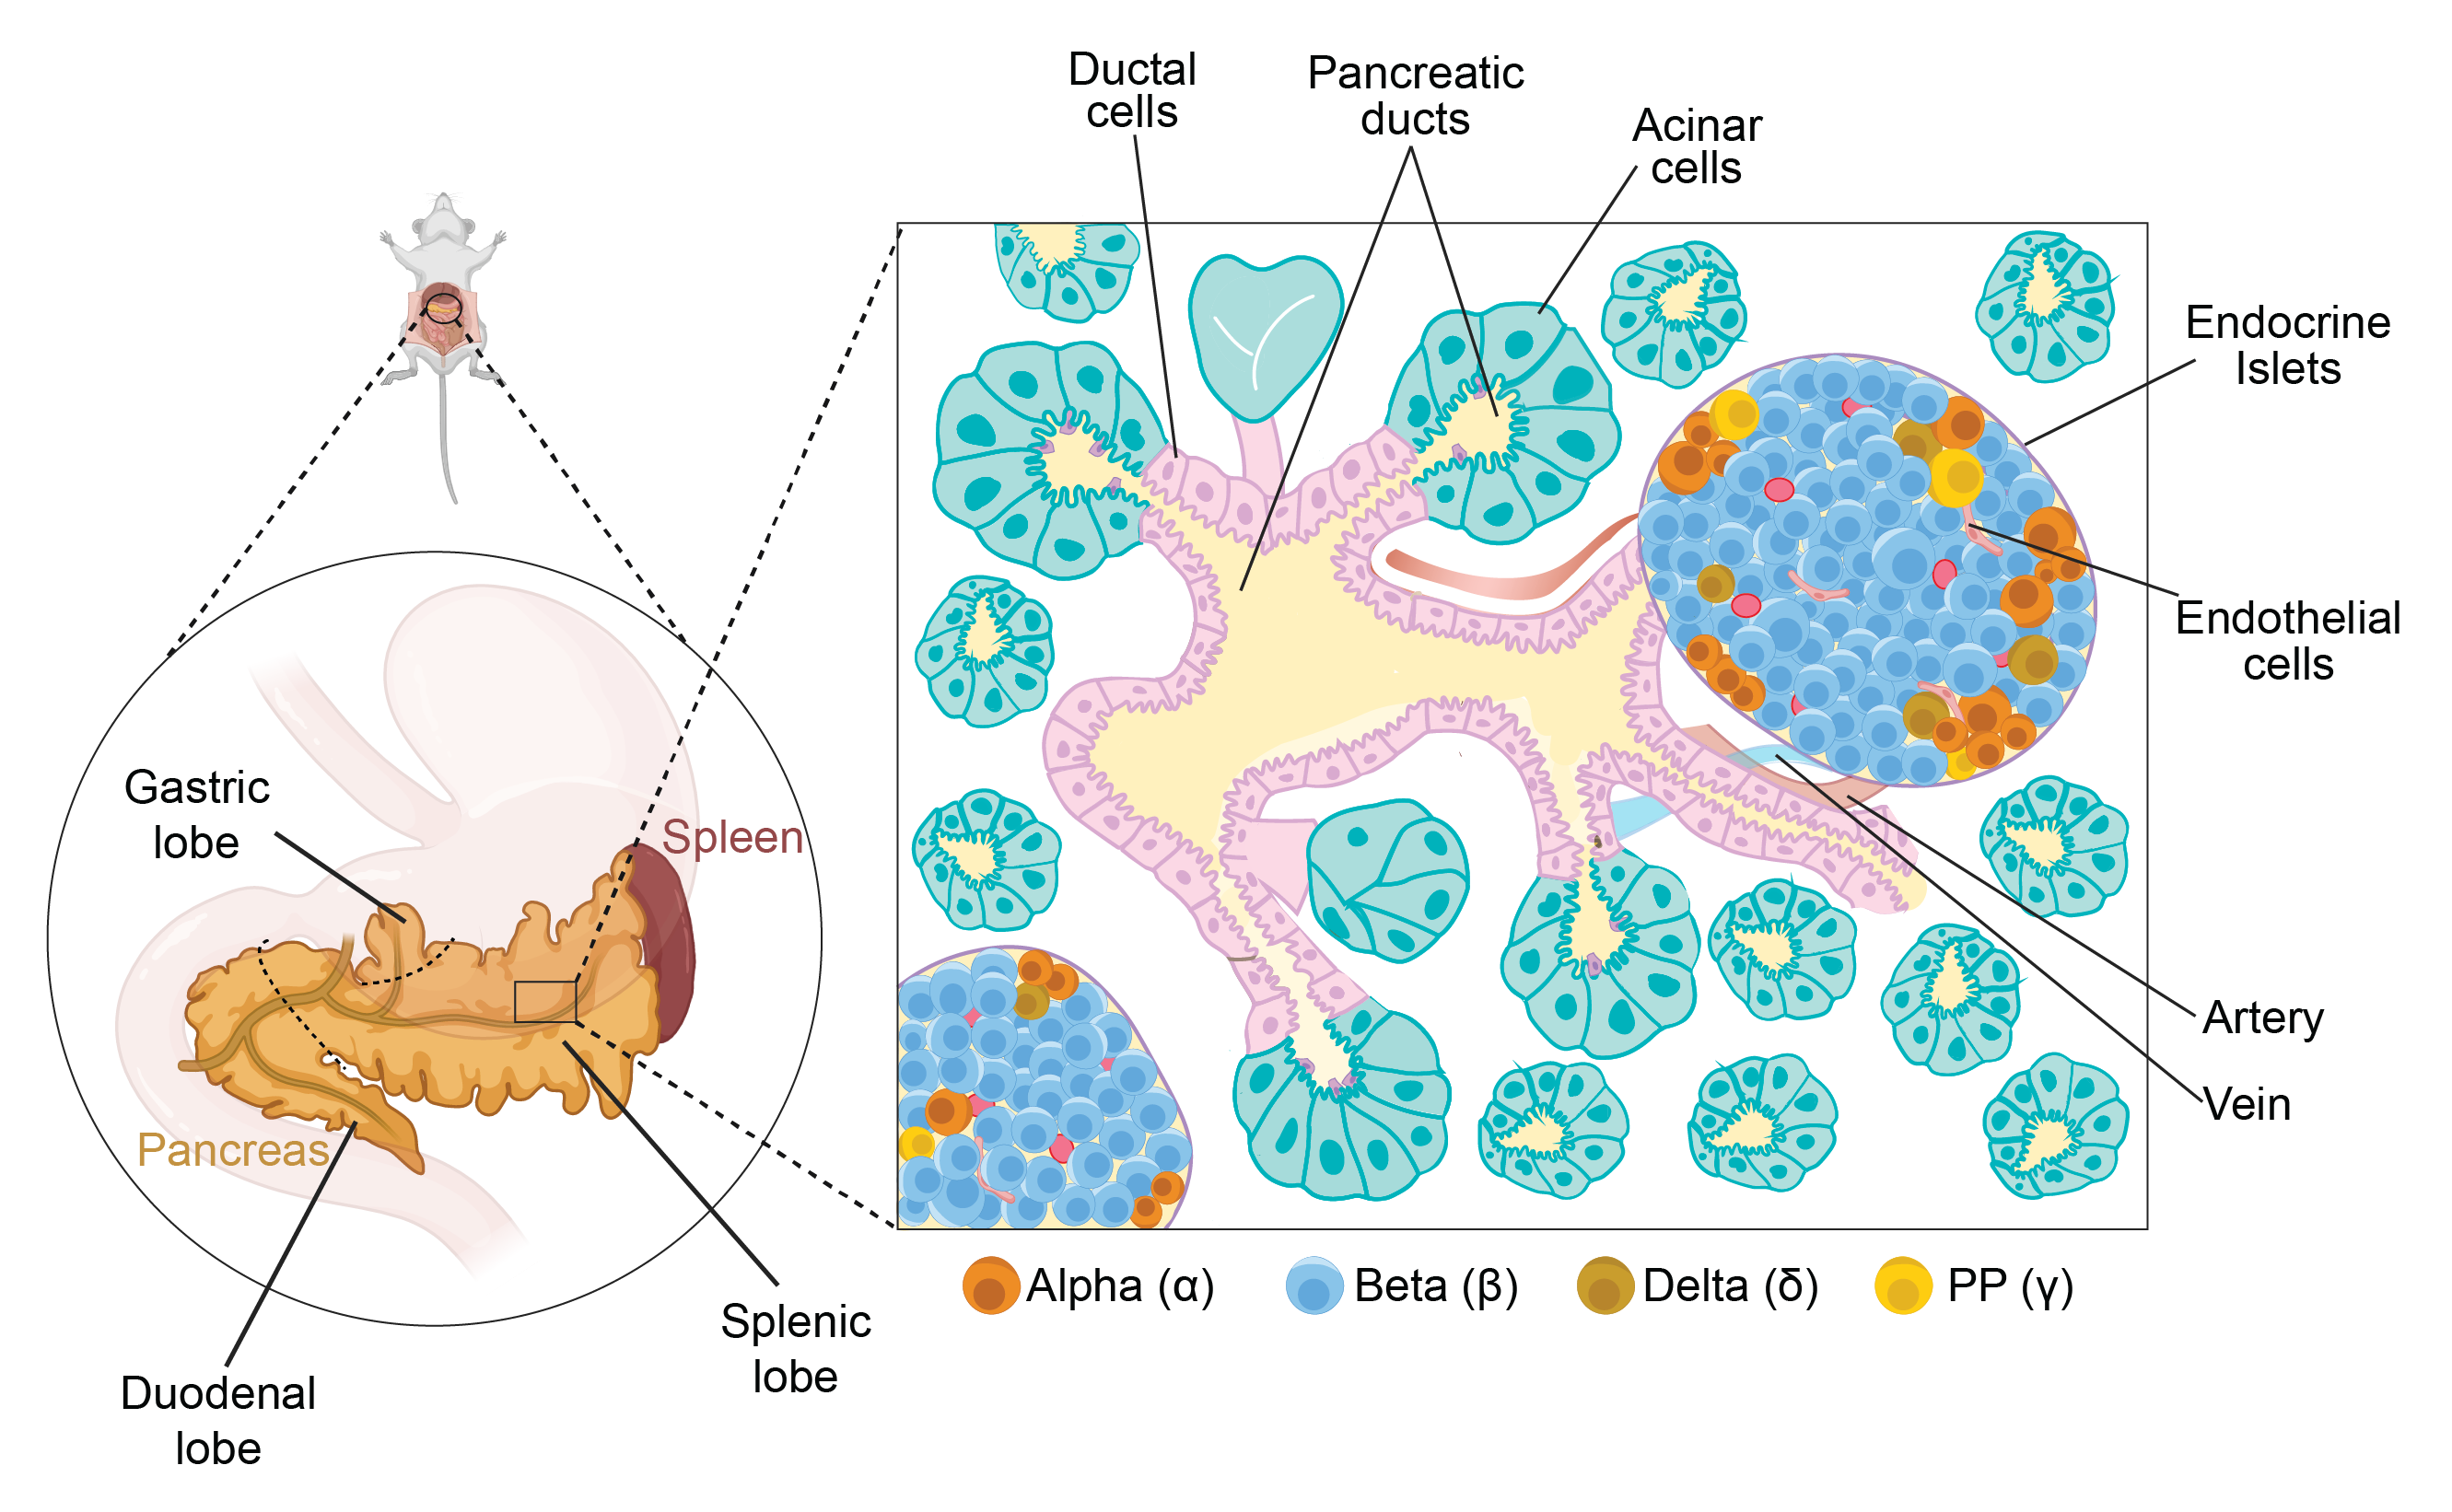
\includegraphics[width=\linewidth]{Chapter1/Fig/F1-1-01.png}
\caption[sec1-1endopanc]{\textbf{Endocrine Pancreas}}
\label{fig1-1}
\end{figure}



The pancreatic tissue in mice is a diffused lobular organ consisting of the duodenal, the splenic, and the gastric lobes. In humans, the pancreas exhibits \st{is} a more compact and well-defined structure, comprising of \st{into three major parts:} the head, the body, and the tail. The pancreas receives a rich vascular supply and the macro-vascular network is conserved in humans and rodents \textbf{\cite{muratore_vascular_2021}}. Although the islets comprise 1-2\% of the pancreas, they receive up to 20\% of the pancreatic blood supply \textbf{\cite{muratore_vascular_2021,jansson_glucose-induced_1986}}. \st{The dense vascularization}This remarkable vascularity of islets is necessary for normal islet function and likely explains how fluctuations in blood glucose are \st{sensed} detected, \st{and lead}leading to rapid and \st{large}substantial changes in the secretion of pancreatic hormones.
\\\\
In rodents such as mice, the islets consist of \textasciitilde75–80\% β-cells, forming a rich “core” and \textasciitilde15–20\% α-cells and the rest is made up by the remaining endocrine cells (δ-cells and PP-cells, <10\% and ε-cells, <1\%), forming the “mantle” of the islet. In contrast, the endocrine cells in the human islets seem to be randomly distributed, and have proportionally fewer β-cells (\textasciitilde55-75\%) and more α-cells (\textasciitilde30-45\%), likely suggesting the major role of glucagon secretion in humans. The variability in cell distribution results in more heterotypic contacts between the endocrine cells in human islets \textbf{\cite{walker_human_2021}}. It has been shown in both mice and humans, that the islet architecture is size-dependent, with smaller islets displaying the core-mantle structure and larger islets with more complex organization \textbf{\cite{dolensek_structural_2015}}. Additional differences in the innervation patterns and presence of smooth muscle cells throughout the vascular network also exist between mouse and human islets \textbf{\cite{rodriguez-diaz_autonomic_2011}}. \st{It is likely that these islet architecture differences between mouse and human}These islet architecture differences between mouse and human likely contribute to physiological differences regarding islet function \textbf{\cite{cabrera_unique_2006}}.
\\\\
To summarize, the pancreatic islets are regarded as a coordinated mini-organ that serves as a remarkable regulator, integrating systemic and local cues to fine-tune blood glucose levels by the synthesis and appropriate secretion of several metabolic hormones by the diverse cell types in the islet microenvironment.

% ********************************** % 1.1.1  **************************************
%\subsection{Principles of (Mendelian) Inheritance} %Section - 1.1.1 
%\label{sec:Mendel}

% ********************************** % 1.1.2 **************************************
% \subsection{Genetic Linkage and the birth of modern genetics} %Section - 1.1.2 
% \label{sec:Morgan}




%%%% Box on genetic terms & origin

%\begin{Comment}
%\hspace{-2.5mm}\textbf{Box 1: Genetic terms \& their origin}\label{box:genetic_terms}
%\small
%\begin{itemize}
%    \item \textbf{Alleles} (originally allelomorphs) were defined by Bateson as the units of inheritance described by Mendel \cite{bateson2013mendel}.
%    \item \textbf{Homozygote} and \textbf{heterozygote} were also used by Bateson to describe individuals carrying the same or different alleles.
%    \item The word \textbf{gene} as a term for the Mendelian factors or units of inheritance was introduced by Danish botanist Johannsen \cite{johannsen1911genotype}. 
%    \item Johannsen also introduced the terms \textbf{phenotype}, as the outward appearance of an individual, and \textbf{genotype}, as their genetic traits. 
%    \item The terms \textbf{polygenetic} (today more often simply polygenic), for traits that are governed by multiple genes, and \textbf{pleiotropic}, for genes that affect multiple, seemingly unrelated, phenotypes also made their first appearance at that time. 
%    \item A \textbf{pedigree}, from the French \textit{pied de grue} (crane's foot), is a diagram that depicts the biological relationships between related individuals.    It is often used to look at the transmission of genetic disorders.
%\end{itemize}
%\vspace{3mm}
%\end{Comment}





% ********************************** % 1.1.3  **************************************
% \subsection{The double helix} %Section - 1.1.3
% \label{sec:double_helix}

% ********************************** % 1.1.4  **************************************
% \subsection{Biometrics} %Section - 1.1.4
% \label{sec:biometrics}

% % %********************************** % 1.1.5  **************************************
% \subsection{Towards quantitative genetics} %Section - 1.1.5
% \label{sec:Fisher}



%\newpage

% % %********************************** % 1.1.6  **************************************
% \subsection{Molecular biology and technological advances}
% \label{sec:genetic_timeline}


% \subsubsection{Cracking the code}
% \label{sec:genetic_code}



% \begin{figure}[htbp]
% \centering
% \includegraphics[width=15cm]{Chapter1/Fig/genetic_timeline_draft.png}
% \caption[Genetic Timeline]{\textbf{150 years of genetics}.\\
% Key scientific discoveries in genetics and corresponding technological advancements.
% A number of scientific discoveries, in combination with key advances in technology and statistical modelling, have led to the identification of thousands of genetic variants which are associated to complex and molecular traits \cite{nhgri2003genetic}.
% Several fundamental contributions have been made, from Mendel's peas to the structure of DNA, to large databases cataloguing genetic variation of hundreds of thousands of individuals.
% Here, I have attempted to highlight the key events that led to today's field of quantitative genetics in the GWAS and post-GWAS era.}
% \label{fig:genetic_timeline}
% \end{figure}

% \subsubsection{Sequencing DNA}
% \label{sec:dna_seq}


% \subsubsection{Understanding the genetic basis of disease}
% \label{sec:disease_genetic}


% \phantomsection
% \label{sec:ld}
% Instead, it was proposed that the combined use of \gls{ld}\footnote{LD: the nonrandom allocation of alleles at nearby variants to individual chromosomes as a result of recent mutation, genetic drift or selection, manifest as correlations between genotypes at closely linked markers \cite{mccarthy2008genome}.} and population- (rather than family-) based studies would be more suitable \cite{risch1996future, jorde2000linkage} - thus practically proposing the design for \glspl{gwas} \cite{risch1996future}.
% However, at the time, implementation of \glspl{gwas} was not possible, for two primary reasons.
% First of all, the technology required to genotype thousands to millions of markers in a single experiment for the larger required sample sizes was not available \cite{risch1996future, visscher2012five}.
% Secondly, the distribution and density of genetic polymorphisms across the genome, and the \gls{ld} between genetic variants across different populations, were unknown.\\

% In some sense, population-based association studies can be viewed as an extension of family-based linkage studies, in which the population studied (derived from common ancestors) acts as an extended pedigree and a much greater number of meiotic recombinations will have occurred between the analysed samples.
% As a consequence, \gls{ld} regions are much smaller than within pedigrees of close relatives, thus requiring a more dense panel of genetic markers to be examined \cite{cordell2005genetic}.

% \subsubsection{The Human Genome Project}
% \phantomsection
% \label{sec:hgp}

% In order to study genomic variation, and therefore its role in disease, it was necessary to generate a reference genome.
% This was the goal of the \gls{hgp}, which aimed at sequencing the entire human genome.
% The \gls{hgp} was 
% % perhaps the first 
% a 
% major breakthrough that dramatically changed the landscape of genetics, and was described by United States President Clinton as “an epic-making triumph of science and reason” \cite{clinton2000remarks} at the announcement of its completion.
% Driven by and a driver of technological breakthroughs in \gls{dna} sequencing and genotyping, the \gls{hgp} was a massive international undertaking and a truly collaborative effort; sequencing and analysis took place across twenty centers in six different countries (USA, UK, France, Germany, Japan, China) and took 13 years to complete, costing approximately \$2.7 billion \cite{lander2011initial}.
% Led in the US by then NIH director Francis Collins and by founder of Celera Genomics\footnote{The company Celera Genomics was formed in May 1998, with the objective of sequencing much of the human genome in three years \cite{venter1998shotgun}.} 
% Craig Venter, and with large contributions from the UK, in particular from the Sanger Institute directed by John Sulston (who had first sequenced the genome of \textit{C. Elegans}), the \gls{hgp} was announced as a joint US-UK statement on June 26th, 2000.
% After a first publication in 2001, the project was truly completed on April 25th, 2003, on the 50$^{th}$ anniversary of the Watson and Crick paper describing the helical structure of \gls{dna}.\\

% The \gls{hgp} provided the first map (obtained from the genomes of a small number of individuals) of the $\sim$3 billion bases in the human genome \cite{lander2001initial, schmutz2004quality, hattori2005finishing}, and revealed that human \gls{dna} consists of surprisingly few exons (1.1\% of the genome), whereas introns cover 24\% of the genome \cite{venter2001sequence, lander2001initial}. 
% Additionally, the number of genes was found to be smaller than expected, with around 30,000 being identified in 2001, and circa 21,000 genes being the latest (still debated) estimate at the time that this thesis is written \cite{pertea2018thousands}. 
% Additional breakthroughs in sequencing technologies have expanded and refined the reference genome, which now captures more than 92\% of the genome and provides a landscape of its genes \cite{lander2011initial}.\\

% With a complete map of the human genome in place, genetic variants could now be identified as those bases discovered in an individual that did not match the (reference) base annotated in the human genome map. 
% Common variants, i.e. variants with \gls{maf}\footnote{The frequency of an
% allele at a genetic locus is the proportion of chromosomes in the study sample that carry that allele \cite{laird2010fundamentals}. 
% For a biallelic variant (a variant for which only two possible alleles are observed in the population), the frequency of the less common (minor) allele is called the minor allele frequency (MAF).} larger than 5\%, were called \glspl{snp}. 
% Previous studies had estimated that approximately 0.1\% (1 base per 1,000) of an individual's genome was a polymorphism \cite{wang1998large, li1991low, cargill1999characterization}. 

% These SNPs were scattered across the genome and it was now time to describe what type of variants they were, where in the genome they were located, and what (if any) effect they had on human phenotypes.

% \subsubsection{The International HapMap Project}

% The International HapMap Project was the first effort of its kind to systematically catalogue genomic variation. 
% Additionally, it aimed to characterise the LD structure of the human genome, which would make GWA studies feasible. 
% The HapMap was officially started in October 2002 as a collaboration between research groups and private companies in Canada, China, Japan, Nigeria, the United Kingdom and the United States with the goal of developing a haplotype map (HapMap) of the human genome \cite{international2003international}.
% By genotyping individuals of African (YRI), European (CEU) and East Asian (JPT, CHB) descent, in Phase I HapMap assembled a publicly available database of common variants (\gls{maf}>5\%) in global samples \cite{international2005haplotype}. 
% The HapMap expanded rapidly. 
% By Phase II (2007), the database contained 2.1 million SNPs from the four original populations \cite{international2007second}.
% Phase III (2010) added genotyping from seven additional populations, for a total of over 3 million SNPs in 11 global ancestry groups\footnote{ASW (African ancestry in Southwest USA); CEU (Utah residents with Northern and Western European ancestry from the CEPH collection); CHB (Han Chinese in Beijing, China); CHD (Chinese in Metropolitan Denver, Colorado); GIH (Gujarati Indians in Houston, Texas); JPT (Japanese in Tokyo, Japan); LWK (Luhya in Webuye, Kenya); MEX (Mexican ancestry in Los Angeles, California); MKK (Maasai in Kinyawa, Kenya); TSI (Tuscans in Italy); YRI (Yoruba in Ibadan, Nigeria).} \cite{international2010integrating}.\\ 

% The growing popularity of genetic association studies in parallel with the expansion of the HapMap effort paved the way for the last needed technological breakthrough: microarrays.
% By knowing the genetic location of thousands of variants, commercial companies were able to develop so-called `SNP chips' \cite{meaburn2006genotyping, oliphant2002beadarray}, which allowed for genotyping at specific locations across the genome.
% In parallel, the data generated by the HapMap project enabled calculation of the LD\footnote{Pearson's correlation coefficient squared, $r^2$, is commonly used} between SNPs within the genome, effectively describing the chance that two SNPs will be inherited together \cite{bush2012genome}.
% This enabled the identification of haplotypes and thus a minimal set of SNPs that capture the majority of the haplotype diversity within a population, called `tag SNPs' \cite{international2003international}. 
% The collective LD information gathered by academics in those years \cite{slatkin2008linkage, pe2006evaluating, otto2002resolving} allowed companies such as Affymetrix and Illumina to develop SNP arrays that contained 
% these tag SNPs, effectively capturing information about common variation across a large percentage of the genome while only directly genotyping a few thousand SNPs.\\

%\newpage

% % %********************************** % 1.1.7  **************************************
% \subsection{Genome-wide association studies}
% \label{sec:gwas}

% The data generated by the International HapMap Project combined with development of appropriate chip-based microarray technology, which enabled simultaneous genotyping of more than one million SNPs, led to the first wave of \glspl{gwas} \cite{visscher2012five}.
% \gls{gwas} are a hypothesis-free\footnote{bar the selection of SNPs on the chip. 
% More recently, shallow DNA-seq has been increasingly used as an alternative, making the approach truly hypothesis-free.} approach to test for statistical association between the genotype frequency of common genetic variants (considered one by one across the genome) and a phenotype of interest \cite{mccarthy2008genome}. 
% The development of GWAS was accompanied by great enthusiasm, and the hope that these studies could better our understanding of the genetic underpinning of human disease, leading to improvement of prognosis and acceleration of drug and diagnostics development. \\

% Initially, \gls{gwas} focused on complex phenotypes with binary outcomes, using a case-control design (i.e. diseased vs healthy).
% Then, for each SNP and binary trait, the association was evaluated using a Cochran–Armitage (trend) test, a $\chi^2$ test or a Fisher's exact test comparing the numbers of cases and controls when stratified by their alleles at the locus of interest. 
% The first successful \gls{gwas} was published in 2002 on myocardial infarction \cite{ozaki2002functional}.
% The same design was then applied in a landmark GWA study conducted in 2005 for age-related macular degeneration (AMD), using 96 cases and 50 healthy controls and testing for associations at $\sim$100,000 SNPs \cite{klein2005complement}. 
% In 2007, the Wellcome Trust Case-Control Consortium (WTCCC) published a study where they performed \gls{gwas} on seven different common diseases, using 2,000 cases for each of bipolar disorder (BD), coronary artery disease (CAD), Crohn's disease (CD), hypertension (HT), rheumatoid arthritis (RA), type I and II diabetes (T1D, T2D) and a common set of 3,000 healthy controls, demonstrating the feasibility of the use of a shared set of controls across several traits \cite{wellcome2007genome}.\\

% A year later, in 2008, the \gls{gwas} Catalog was founded to keep a record of all published \gls{gwas} and identified associations \cite{welter2014nhgri}.
% As of September 2020, when I am writing this thesis, the \gls{gwas} Catalog includes 4,694 publications, describing 197,708 SNP-trait associations \cite{macarthur2017new}.\\

% Over time, quantitative traits have become increasingly popular to use as phenotypes, in addition to binary traits.
% These include continuous traits such as height, weight and blood pressure.
% Furthermore, linear regressions and their derivations have become more popular methods to assess association, due to their flexibility to include covariates \cite{mccarthy2008genome}.
% I describe these models in detail in the next chapter (\textbf{Chapter \ref{chapter2}}). 

%\newpage

% \gls{gwas} results are often visualised using a Manhattan plot \cite{mccarthy2008genome}, where the negative log p value (as a measure of significance) is plotted on the y axis, against the corresponding genomic position (ordered by chromosome and position) on the x axis (\textbf{Fig. \ref{fig:manhattan}}). 
% Peaks on these plots represent loci (multiple variants in \gls{ld}) that display evidence of association with the analysed phenotype. 
% Variants are deemed to be significantly associated with a trait if they exceed an appropriately chosen p value threshold. 

%\begin{figure}[h]
%\centering
%\includegraphics[width=15cm]{Chapter1/Fig/Manhattan_plots_CD_WTCCC_2007.jpg}
%\caption[Manhattan plot]{\textbf{Manhattan plot}.\\
%Manhattan plot for Crohn's disease (CD) from the WTCCC study \cite{wellcome2007genome}.
%On the x axis are plotted the genomic positions of the SNPs tested, one chromosome after %the next.
%On the y axis are the association significance values.  
%Alternating colours are used to distinguish chromosomes (odd numbered chromosomes -and chromosome X- are dark, even numbered chromosomes are light).
%Highlighted in green are statistically significant SNPs (p value < $5 \times 10^{-8}$).}
%\label{fig:manhattan}
%\end{figure}

%\subsubsection{From global traits to molecular traits}

 

% % %********************************** % 1.1.8  **************************************
% \subsection{Expression quantitative trait loci}
% \label{sec:eqtl}

% \subsubsection{Mechanisms of the genetic regulation of gene expression}


% \subsubsection{Mapping eQTL}
% \label{sec:eqtl_map}

 
 
% \subsubsection{\textit{Cis} and \textit{trans} eQTL}



% \begin{figure}[h]
% \centering
% \includegraphics[width=15cm]{Chapter1/Fig/eqtl.png}
% \caption[\textit{Cis} and \textit{trans} eQTL]{\textbf{\textit{Cis} and \textit{trans} eQTL}.\\
% \textit{Cis} eQTL affect the expression of genes directly. 
% \textit{Trans} eQTL, in contrast, affect the expression of typically more distant genes, often by first having a \textit{cis} effect on the expression of intermediate regulatory genes.
% % On the right, the typical representation of eQTL using box plots.
% Figure adapted from \cite{westra2014genome}.
% }
% \label{fig:eqtl}
% \end{figure}



% \subsubsection{From tissue-specific to cell type-specific eQTL}
% \label{sec:eqtl_celltype_specific}



% \subsubsection{Context-specific eQTL}


% \newpage

% \subsubsection{Using eQTL to link genes to disease}
% \phantomsection
% \label{sec:eqtl_gwas}



% \subsubsection{eQTL mapping in iPSC and iPSC-derived cells}



% ***********************************************************************************************************************************************************************************************************************************************************************************************************************************

\newpage

% \vspace*{10px}

% \textit{“It is not birth, marriage, or death, but gastrulation which is truly the most important time in your life.”}\\
% \rightline{Lewis Wolpert, 1986}

% \vspace*{5px}

% ***************************************************************
%************************ %Second Section %****************************************************************
\section{ Islet \( \mathbf{\upbeta} \)-cells}  %Section - 1.2
\label{sec:human_ipscs}  

% ********************************** % 1.2.1  **************************************
\subsection{Pancreas Organogenesis} %Section - 1.2.1 
\label{sec:pancorgano}

Pancreas organogenesis is a \st{highly} conserved process during fetal development and comprises a tightly coordinated and regulated interplay of complex signaling events. During this step-wise program, the pancreas develops from a simple bud-like structure to a \st{final} mature, highly branched organ containing several specialized cell types. In mice, the pancreas specification begins at embryonic day 8.5 \textbf{(e8.5)} with the formation of dorsal and ventral pre-pancreatic regions in the foregut endoderm \textbf{\cite{shih_pancreas_2013, slack_developmental_1995}}. The pancreas development becomes morphologically evident at  \textbf{\textasciitilde e9.5} when the presumptive pancreatic regions in the endoderm undergo thickening and eventually result in the emergence of pancreatic buds \textbf{\cite{shih_pancreas_2013}}. Over the next 2-3 days, the pancreatic buds continue to elongate, accompanied by the stratification of the epithelium and the formation of multiple micro-lumens \textbf{\cite{pan_pancreas_2011}}. At \textbf{\textasciitilde e12.5}, as a result of both due to gut rotation and elongation of the dorsal and ventral stalks, the pancreatic buds (dorsal and ventral) come into contact and fuse into a single organ. \textbf{This early phase of pancreatic development is referred to as the “primary transition”.}
\\\\

% ********************************** % 1.2.2  **************************************
\subsection{Endocrine Cell Development} %Section - 1.2.2 
\label{sec:endodev}
The vast majority of the endocrine cells arise during the secondary transition from the endocrine progenitors \textbf{\cite{pan_pancreas_2011}}. However, glucagon-containing α-cells can be seen as early as \textbf{e9} in the primordium \textbf{\cite{pictet_ultrastructural_1972,gittes_developmental_2009}}. The fate decision in the bi-potent trunk domain during the secondary transition is determined by graded \textit{Notch} activity. Lower \textit{Notch} activity leads to \textit{Sox9} expression, which is an activator of \textit{Ngn3} \textbf{\cite{shih_pancreas_2013}}, a basic-helix-loop-helix \textbf{(bHLH)} transcription factor \textbf{(TF)} and master regulator of endocrinogenesis \textbf{\cite{gu_direct_2002}}. Cells that do not escape \textit{Notch} signaling express both \textit{Hes1} and \textit{Sox9}, resulting in \textit{Ngn3} repression and eventual contribution to the ductal tree. \st{However, no signals have yet been identified that could account such a segregated expression pattern of Ngn3.} After \textit{Ngn3} expression, endocrine progenitors exit the cell-cycle and delaminate into surrounding stromal tissue \textbf{\cite{shih_pancreas_2013, gouzi_neurogenin3_2011, miyatsuka_neurogenin3_2011}}. These \textit{Ngn3+} cells are uni-potent and as a whole can generate the five different endocrine cell types \textbf{\cite{shih_pancreas_2013,gu_direct_2002,miyatsuka_neurogenin3_2011}}. The timing and strength of \textit{Ngn3} expression determines the efficiency of endocrine cell formation and the cell type: early \textit{Ngn3} expression results in formation of α-cells while delayed expression of \textit{Ngn3}  generates β- and δ-cells followed by γ-cells\textbf{\cite{johansson_temporal_2007}}.
\\\\
Critical TFs such as \textit{Pax4}, \textit{Pdx1} and \textit{Nkx6.1} control the determination of β-cell fate. On the contrary, \textit{Arx} determines α-cell identity. Both \textit{Pax4} and \textit{Arx} are targets of \textit{Ngn3} and are co-expressed, after which they begin to repress each other. In the \textit{Nkx6.1+} β-cell precursors, the switch from the TF \textit{MafB} \st{(v-Maf avian musculoaponeurotic oncogene homolog B)} to \textit{MafA} expression is an important step to activate the complete the β-cell specific program. After birth, immature β-cells undergo stepwise maturation to become fully mature cells.
\\\\
% ********************************** % 1.2.3  **************************************
\subsection{Postnatal \( \mathbf{\upbeta} \)-cell maturation} %Section - 1.2.3
\label{sec:betamat}
β-cell maturation is continuation of β-cell development and occurs postnatally in mammals (https://link.springer.com/article/10.1007/s00125-022-05672-y). Most of the current understanding of β-cell maturation process is derived from neonatal rodent islets, as similar data from humans is difficult to collect \textbf{\cite{liu_all_2017, salinno_-cell_2019}}. After birth, immature β-cells undergo several steps to become fully mature and functional cells characterized by tightly controlled insulin secretion in response to glucose.
\\\\
The immature β-cells are organized into clusters, forming proto-islets \textbf{\cite{salinno_-cell_2019}}, which eventually undergo structural rearrangements to form the compacted core and mantle architecture \textbf{\cite{sharon_peninsular_2019}}. The developmentally immature β-cells are characterized by a strong proliferative capacity, thereby resulting in a general increase in β-cell mass. The immature β-cells present insulin granules but display “leaky” insulin secretion wherein they have a decreased glucose threshold for stimulated insulin secretion \textbf{\cite{liu_all_2017, blum_functional_2012}} and are less glucose-responsive thereby affecting their ability to regulate insulin secretion in response to fluctuating blood glucose levels. \st{[ref]. <continue from PAI>}
\\\\
Immature β-cells follow a biphasic pattern of maturation \textbf{\cite{salinno_-cell_2019, stolovich-rain_weaning_2015}}.  The first wave starts right after birth and lasts until \textasciitilde 2 weeks, during which β-cells increase the expression of several key TFs and associated machinery necessary to establish adult β-cell identity. Some of the key signature genes include \textit{Pdx1}, \textit{Neurod1}, \textit{Nkx2.2} and \textit{Nkx6.1}, which are expressed by all β-cells at birth \textbf{\cite{salinno_-cell_2019}}. In addition, several other markers have also been identified which mark the early phase of functional maturation of β-cells: increased expression of \textit{Ucn3} \textbf{\cite{salinno_-cell_2019, blum_functional_2012}}, \textit{Syt4} \textbf{\cite{salinno_-cell_2019, huang_synaptotagmin_2018}}, \textit{Fltp} \textbf{\cite{salinno_-cell_2019, bader_identification_2016}}  and dramatic drop in levels of \textit{Npy} \textbf{\cite{salinno_-cell_2019, rodnoi_neuropeptide_2017}}. Among TFs, \textit{MafA} progressively substitutes \textit{MafB} expression and further regulates expression of genes involved in glucose sensing and insulin secretion, thereby characterizing the late phase of postnatal maturation.
\\\\
The second wave of maturation occurs from about the third week of life until the weaning period involving dietary change from high-fat maternal milk to a high-carbohydrate chow diet. During this weaning phase, β-cells begin to exhibit improved glucose-stimulated insulin secretion and glucose-induced replication, although the latter remains to be explained. This phase is characterized by β-cells differentially regulating metabolic pathways, involving a switch from mTORC1 to AMPK-dependent signaling, which defines the mature functional landscape. The dietary change associated with the weaning period also affects the secretion of incretin hormones, which enhance GSIS and modulate β-cell replication.
\\\\
% ********************************** % 1.2.4  **************************************
\subsection{Insulin Biosynthesis} %Section - 1.2.4
\label{sec:insbio}
Blah blah blah
\\\\
% ********************************** % 1.2.5  **************************************
\subsection{Glucose-Stimulated Insulin Secretion (GSIS)} %Section - 1.2.5
\label{sec:gsis}
blah blah blah
\\\\
% ********************************** % 1.2.6  **************************************
\subsection{Regulation of GSIS} %Section - 1.2.6
\label{sec:reggsis}
blah blah blah
\\\\
% ********************************** % 1.2.7  **************************************
\subsection{Insulin Action and Clearance} %Section - 1.2.7
\label{sec:insact}
Insulin exerts its known physiological effects by binding to the insulin receptor (InsR) on the surface of target cells. The InsR assembles as a tetramer, consisting of two extracellular alpha subunit, which binds insulin and a two membrane-spanning beta subunit, with a tyrosine-kinase domain each. The activation of this kinase results in a metabolic signaling cascade downstream, eventually leading to the uptake of glucose, lipids and amino acids into the cells. The two principal pathways resulting from this interaction include the phosphoinositide 3-kinase (PI3K)/Akt pathway and the Ras/mitogen-activated protein kinase (MAPK) pathway. The PI3K/Akt pathway is critical for linking insulin receptor substrate (IRS) proteins to the metabolic actions of insulin whereas the Ras/MAPK pathway is primarily associated with the growth and mitogenic effects of insulin \textbf{\cite{de_meyts_insulin_2000}}. The binding of insulin to InsR in the target tissues stimulates the translocation of glucose transporter 4 (GLUT4) storage vesicles from intracellular pools to the cell surface, thereby increasing the rate of glucose uptake \textbf{\cite{shepherd_glucose_1999,saltiel_insulin_2001,leto_regulation_2012}}. In the absence of insulin, only ~5\% of GLUT4 pool can be found on the plasma membrane \textbf{\cite{leto_regulation_2012}}.
\\\\


% %********************************** % 1.2.1  **************************************
% \newpage

% \subsection{From homunculi to developmental biology}
% \label{sec:history_developmental_biology}



% \begin{wrapfigure}{r}{0.6\textwidth}
% \includegraphics[width=9.5cm]{Chapter1/Fig/Early_theories_development.png}
% \caption[Early theories of development]{\textbf{Early theories of development}.\\
% Illustration of the two leading theories on human embryology before the 19$^{th}$ century.
% Left, Illustration of Preformation: 
% A tiny person (homunculus) growing inside a sperm, as drawn by Nicolaas Hartsoeker in 1695.
% Right, Epigenesis: study of foetus deveopment by Leonardo Da Vinci, c. 1510.}
% \label{fig:early_embryology}
% \end{wrapfigure}




\newpage

% \subsection{}}
% \label{sec:human_embryogenesis}




% \begin{figure}[h]
% \centering
% \includegraphics[width=14.5cm]{Chapter1/Fig/embryogenesis_til_gastrulation.png}
% \caption[Human Embryogenesis]{\textbf{Human Embryogenesis}.\\
% Early stages of human embryogenesis.
% (a) From zygote to morula: stages of clevage.
% (b) The blastocyst.
% Cells divide and form an outer layer, the trophoblasts.
% Inner cells also called embryoblasts get compacted and move to a side forming the inner cell mass (ICM), leaving a fluid filled cavity called the blastocoel.
% (c) The formation of the bilaminar disk.
% The ICM splits into the epiblast and hypoblast which distribute along the surface and result into two more cavities, the amniotic cavity and the primitive yolk sac, respectively.
% (d) Gastrulation: from bilaminar to trilaminar disk.
% The primitive streak forms and cells start to migrate moving down in between the epiblast and the hypoblast.
% The endoderm, mesoderm and ectoderm form and are called the trilaminar disk.}
% \label{fig:embryogenesis}
% \end{figure}

 

% \subsection{Human Stem Cells}
% \label{sec:escs} 


% \begin{figure}[htbp]
% \centering
% \includegraphics[width=16cm]{Chapter1/Fig/stem_cell_potency.png}
% \caption[Stem Cells]{\textbf{The potency tree of stem cells}.\\
% The spectrum of potency along human development: from the totipotent zygote to terminally differentiated cells.}
% \label{fig:stem_cells}
% \end{figure}

% \subsubsection{Embryonic stem cells}
% \label{sec:esc_induction}




% %********************************** % 1.2.3  **************************************
% \subsection{Nuclear cloning of somatic cells}
% \label{sec:cloning} 


% %********************************** % 1.2.1  **************************************
% \subsection{Induced pluripotent stem cells}
% \label{sec:ipsc}
   

%\begin{figure}[h]
%\centering
%\includegraphics[width=15cm]{Chapter1/Fig%/ipsc_timeline.png}
%\caption[iPSCs timeline]{\textbf{Historical timeline of key events leading to the development of iPS cells}.\\
%Key events including somatic cloning and isolation of ES cells that eventually led Shinya Yamanaka and colleagues to generate iPSCs in 2006 and Yamanaka to win the 2012 Nobel Prize for Physiology and Medicine alongside Sir John Gurdon.}
%\label{fig:ipsc_timeline}
%\end{figure}

% \newpage

% \subsubsection{Inducing pluripotency}

% \subsubsection{Challenges in the use of iPSCs}
% \subsubsection{Reprogramming factors}
% \subsubsection{Mechanisms of iPSC induction}



%\begin{figure}[htbp]
%\centering
%\includegraphics[width=14cm]{Chapter1/Fig/ipscs.png}
%\caption[iPS cells]{\textbf{iPS cells - derivation and applications}.\\
%The generation of iPSCs starts with a biopsy from, for example, the skin of an adult donor.
%Adult cells, in the example fibroblasts, are then isolated and pluripotency is induced through four reprogramming factors, for example the Yamanaka factors: Oct4, Sox2, Klf4 and c-Myc (OSKM).
%The factors can be delivered using a number of systems, see \textbf{page \pageref{sec:ipsc_delivery}}.
%The resulting induced pluripotent stem cells (iPSCs) are self-renewing and are virtually indistinguishable from ESCs.
%They can be subsequently differentiated towards other cell types, including disease relevant cell types, for example dopaminergic neurons for Parkinson's disease, or pancreatic beta cells for diabetes.
%In the future, iPSC-derived cells might be used for cell therapy, i.e. they could be transplanted into the patient, with no risk of allogenic rejection.
%In the meantime, iPSCs and iPSC-derived differentiations can be used to model development and disease, and to do compound screening and drug testing.
%Figure created with BioRender.com.}
%%\label{fig:ipsc}
%\end{figure}


% \subsubsection{Delivery methods}
% \label{sec:ipsc_delivery}




% \subsubsection{Somatic cell of origin}
% \label{sec:ipsc_somatic_cell}



% \subsubsection{Characterising iPSCs}
% \label{sec:ipsc_characterise}



% \subsubsection{Heterogeneity of iPSCs and between cell line variation}


% \subsection{Applications of human iPSCs in genetics}
% \label{sec:ips_genetics}





% \subsubsection{HipSci and other human iPSC consortia}
% \label{sec:HipSci}


% \subsubsection{eQTL mapping using iPSCs and iPSC-derived cells}


% \newpage

% %********************************** %Third Section  **************************************
\section{Diabetes Mellitus}


Diabetes Mellitus (DM), commonly referred to as diabetes, is a group of complex metabolic disorders that has reached pandemic proportions, and poses a significant global health challenge. \st{As of 2019, approximately 463 million adults aged 20-79 were diabetic and this number is projected to rise to ~700-800 million by 2045.} The International Diabetes Federation (IDF) reported that 10.5\% of the adult population (20-79 years) had diabetes in 2021, and projected that this proportion would increase to 13.7\% by 2045 \cite{home_idf_nodate}. In Germany, an estimated 7\% of the adult population was diabetic in the year 2021 \cite{noauthor_germany_nodate}. Diabetes is associated with several long-term complications such as kidney failure, cardiovascular diseases and is a major risk factor for blindness, lower limb amputation, \st{stroke}and stroke and nerve damage \cite{ashcroft_diabetes_2012,emerging_risk_factors_collaboration_diabetes_2010,leon_diabetes_2015}. Consequently, diabetes stands as one of the foremost causes of global mortality \st{Altogether, this makes diabetes a leading cause of mortality worldwide} with 6.7 million deaths in 2021 \cite{home_idf_nodate}. These premature deaths and comorbidities \st{due to diabetes} inflict a huge economic strain on healthcare systems. The IDF estimated an expenditure of at least USD 966 billion in diabetes related causes in 2021 \cite{home_idf_nodate}. To address this burgeoning crisis and mitigate risk factors a multifaceted approach is essential with research efforts directed towards unraveling the complex interplay of genetic, environmental, and lifestyle factors that contribute to the development of diabetes. 

% ********************************** % 1.3.1  **************************************
\subsection{Forms of Diabetes} %Section - 1.3.1 
\label{sec:forsmDiabets}

DM \st{Diabetes mellitus (short - diabetes)} is \st{a group of complex metabolic disorders} characterized by sustained high blood glucose concentrations (hyperglycemia) \st{because of insufficient supply of insulin} resulting from inadequate insulin production, impaired insulin action, or a combination of both. Diabetes is broadly classified into two main types: Type 1 and Type 2  The current classification relies both disease etiology and pathogenesis \textbf{\cite{banday_pathophysiology_2020}}, serving as a valuable tool in clinical disease assessment and therapy determination. Based on this, diabetes can be divided into four main categories:\\
\begin{enumerate}
    \item Type 1 DM \textbf{(T1DM)}
    \item Type 2 DM \textbf{(T2DM)} 
    \item Gestational DM \textbf{(GDM)} and 
    \item Diabetes associated with certain specific conditions and/or disorders.
\end{enumerate}


%\begin{figure}[htbp]
\begin{figure}[t]
\centering
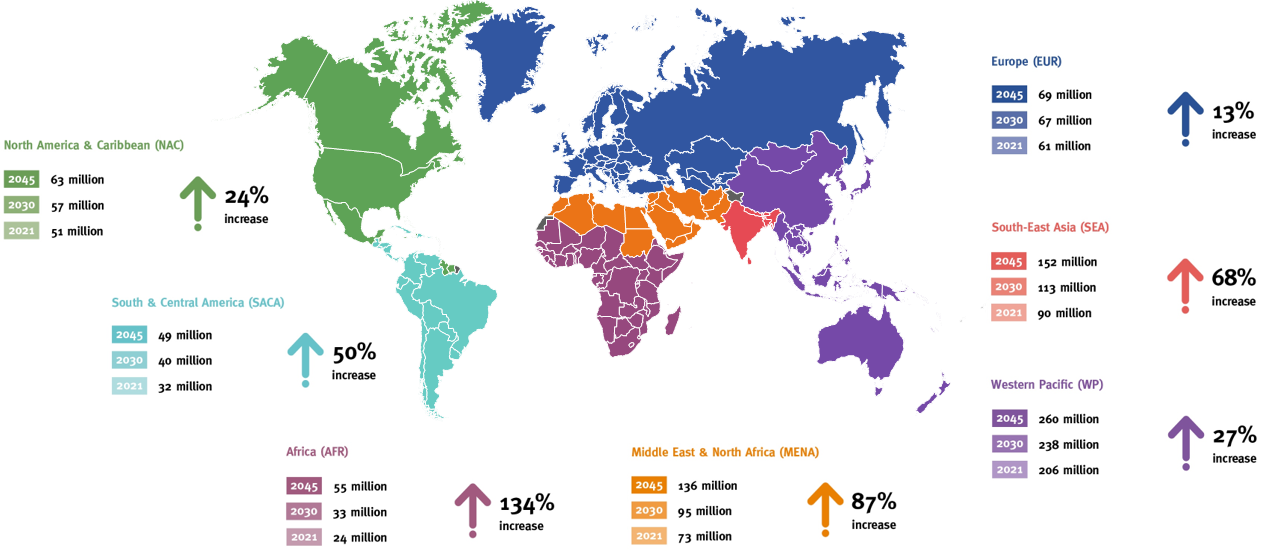
\includegraphics[width=14cm]{Chapter1/Fig/IDF.png}
\caption[diabetes]{\textbf{IDF Atlas 2021}.\\\\
The generation of iPSCs starts with a biopsy from, for example, the skin of an adult donor.
Adult cells, in the example fibroblasts, are then isolated and pluripotency is induced through four reprogramming factors, for example the Yamanaka factors: Oct4, Sox2, Klf4 and c-Myc (OSKM).}
%\label{fig:ipsc}
\end{figure}

\subsubsection{T1DM}

Type 1 DM (T1DM) is a chronic, autoimmune disorder in which the insulin-secreting \textbeta-cells are progressively lost, and immune cell infiltration into the pancreatic islets play a crucial role in this process. The destruction of \textbeta-cells, caused by auto-reactive CD4 and CD8 T-cells results in little to no insulin production causing hyperglycaemia. As the disease progresses, auto-antibodies targeting \textbeta-cell proteins, especially native insulin, manifest and are subsequently joined by auto-antibodies against other proteins (glutamic acid decarboxylase or zinc transporter 8), leading to an expansion of auto-reactivity and eventual development of overt clinical disease (marked by destruction of 85-90\% of \textbeta-cells).
\\\\
T1DM is typically presents during diagnosed in childhood and adolescence,\st{but not exclusively, and accounts for 5-10\% of all cases of diabetes} although it can occur at any age, contributing to 5-10\% of all diabetes cases \textbf{\cite{banday_pathophysiology_2020}}. The etiology of T1DM is multifactorial, involving both, genetic predisposition and environmental triggers \st{play an important role in in its the pathogenesis. of T1DM}. The current therapeutic strategy entails daily exogenous administration of insulin to maintain stable glucose levels. Alternative approaches include a hybrid-closed loop model (artificial pancreas) for regulated insulin delivery, primary islet transplantation or immuno-modulation, albeit, the latter two present their own set of challenges. Additionally, early clinical trials involving stem cell therapies, such as mesenchymal stem cell (MSC) therapy have shown promising results as potential treatments for T1DM \textbf{\cite{pathak_therapies_2019}}.

\subsubsection{T2DM}

Type 2 DM (T2DM) develops from high insulin demand due to insulin resistance in peripheral target tissues. The insulin resistant state manifests several years prior to T2DM diagnosis. Functional β-cells can match the increased metabolic demand by secreting more insulin in order to maintain normal glucose levels. However, sustained demand over chronic periods leads to progressive β-cell dysfunction, resulting in glucose intolerance and overt disease. \textbf{Insulin resistance and β-cell dysfunction are considered as major hallmarks of T2DM \cite{banday_pathophysiology_2020}}. 
\\\\
While, genome-wide association studies (GWAS) have been able to identify the genetic susceptibility to T2D \textbf{\cite{grarup_genetic_2014, wang_genetic_2016}}, other factors, particularly obesity have demonstrated a strong link to insulin resistance and T2DM pathogenesis. Excessive obesity causes a metabolic overload of the adipose tissue, resulting in chronic inflammation via secretion of pro-inflammatory cytokines such as TNF-a, IL-6, IL-1B and MCP-1 \textbf{\cite{guilherme_adipocyte_2008}}. The macrophages recruited into the adipose tissue create a chronically inflamed state and reduce the uptake of fatty acids by skeletal muscle. The elevated levels of these free fatty acids impair signaling and insulin-stimulated glucose transport leading to the development of insulin resistance \textbf{\cite{unger_lipotoxicity_1995,uysal_protection_1997,kanda_mcp-1_2006}}. However, the critical determinant for T2D is β-cell dysfunction \textbf{\cite{tahrani_glycaemic_2010, khin_pancreatic_2023}}, which is more severe than insulin resistance. The interplay between β-cell dysfunction and insulin resistance is highly complex; however, they likely influence each other and synergistically worsen T2DM.  Several factors are thought to contribute to β-cell dysfunction – chronic nutrient overload (glucotoxicity and glucolipotoxicity) \textbf{\cite{prentki_nutrient-induced_2020}}, insulin secretory defects \textbf{\cite{kahn_mechanisms_2006}}, reduced β-cell mass, amyloid deposition \textbf{\cite{prentki_islet_2006}} and/or islet inflammation and oxidative stresses. \st{The role of islet inflammation in T2D and its involvement in β-cell dysfunction is discussed at length in Chapter 2.}
\\\\
T2DM accounts for 90-95\% of all diagnosed diabetic cases53,57,70. Due to the multi-faceted and progressive nature, the treatment for T2D follows a step-wise approach. The very first recommended therapeutic intervention is the adoption of a healthier life style: more healthy diet, increased physical activity and maintaining a healthy body weight. The first anti-diabetic drug to be usually prescribed is Metformin, which works by reducing hepatic gluconeogenesis, delaying intestinal absorption and improving the overall insulin sensitivity71, although accumulating evidence points to possible new mechanisms of actions72. The persistence of T2DM further requires a additional medications as monotherapy is insufficient to maintain normal blood glucose levels53,73. Other available anti-diabetic drugs include sulphonylureas, glucagon-like peptide 1 (GLP-1) agonists, thiazolidinediones, sodium-glucose cotransporter 2 (SGLT2) inhibitors or dipeptidyl peptidase 4 (DPP-4) inhibitors 53,73,74. Upon failure of these antidiabetic drugs, intensive insulin therapy via exogenous administration becomes necessary in order to maintain the target range of blood glucose levels in T2DM patients and avoid health complications 53.
\\\\
T1DM and T2DM together account for most of the diabetes cases. Besides these two, there are also less common forms of diabetes:


%The overall aim of this thesis is to provide suitable computational methods for the identification of cell type and context-specific eQTL using single cell expression profiles, and explore their application across a range of human iPSC-derived cell types, using data from the \gls{hipsci} project.\\

%Specifically, in \textbf{Chapter \ref{chapter2}}, I provide an overview of the use of linear and \glspl{lmm} for genetic association analyses, focusing on their application in \gls{eqtl} mapping.\\

%In \textbf{Chapter \ref{chapter3}}, I describe best-practice approaches to perform \gls{eqtl} mapping using \gls{scrnaseq} profiles and demonstrate these methods on matched bulk and single cell expression of around 100 human \gls{ipsc} lines. \\

%In \textbf{Chapter \ref{chapter4}}, I present a dataset of almost 40,000 cells from 125 human \gls{ipsc} lines differentiating to definitive endoderm, and demonstrate different approaches to \gls{eqtl} mapping using \gls{scrnaseq} data, identifying genetic variants that affect gene expression dynamically along differentiation and across other cellular states. \\

%In \textbf{Chapter \ref{chapter5}}, I present a dataset of over one million cells from 215 human \gls{ipsc} lines differentiating to midbrain dopaminergic neurons. We identify thousands of \glspl{eqtl} across a number of cell types and upon external stimulation. In addition, we identify hundreds of colocalisation events with variants that are known to be associated with neurological traits and diseases. Moreover, we investigate sources of variation in the capacity of individual cell lines to differentiate toward neurons.\\

%Finally, in \textbf{Chapter \ref{chapter6}}, I conclude and discuss future directions.
\newpage

% ***************************************************************
%************************ %Fourth Section %****************************************************************
\section{scRNA-seq}  %Section - 1.4
\label{sec:scrna} 

\subsection{Introduction}
\label{sec:141}


\subsection{Other Modalities}
\label{sec:142}

Besides single-cell transcriptomics, a range of other technologies aims to profile the distinct layers contributing to the overall molecular make-up of a cell. Collectively, these single-cell methodologies enable us to uncover cellular diversity from novel perspectives, offering comprehensive and impartial analyses of individual cells \textbf{\cite{stein_single-cell_2021}}. Some of these modalities are:

\subsubsection{Single-cell multi-omics}


%\chapter{Aims}
\label{chp:aims}

\newpage\null\thispagestyle{empty}\newpage

\par The work presented in this thesis is focused on investigating two crucial topics in the field of \acrfull{t2d} pathogenesis:\\

\textbf{\underline{Obesity, aging and pancreatic inflammation}}
\vspace{15pt}
\par Chronic nutrient excess leads to progressive dysfunction of insulin-secreting $\beta$-cells, resulting in glucose intolerance and eventually \glsentryshort{t2d}. Another risk factor for the development of \glsentryshort{t2d} is aging, and both are associated with a chronic, low-grade inflammation in metabolic tissues, including pancreatic islets. Islet inflammation is a hallmark of \glsentryshort{t2d} development and pathology. However, a detailed survey of how nutrient excess and aging impacts immune cell dynamics within the islets is lacking.\\

\par The goal of this project was to conduct in-depth and integrative data analysis from multi-parametric technologies such as \glsentrylong{scr} (\glsentryshort{scr}) and imaging mass cytometry (\glsentryshort{imc}) to assess the impact of obesity (induced by a a\glsentrylong{wd}) and aging on CD45\textsuperscript{+} immune cells in pancreas and pancreatic islets. The multi-modal approach provided a spatio-temporal profile of immune cell dynamics, revealing diet-specific and age-specific inflammatory patterns and their roles in the development of \glsentryshort{t2d}. The findings from this chapter emphasized the necessity of considering both dietary and age-related factors in diabetes research to understand their combined effects on pancreatic inflammation and disease progression.\\

\textbf{\underline{$\beta$-cell sub-populations and metabolic stress responses}}
\vspace{15pt}
\par Heterogeneity in $\beta$-cells is crucial for adaptive and compensatory responses in face of metabolic challenges. While \glsentryshort{scr} studies have detailed this heterogeneity, there is a general lack of consensus on the number of $\beta$-cell sub-populations and their interrelationships. Furthermore, a thorough understanding of how $\beta$-cells initiate adaptive responses and how they fail due to unresolved stress is lacking.\\

\par The goal of this project was to perform a comprehensive analysis of the heterogeneous $\beta$-cell subsets across various models of $\beta$-cell adaptation and decompensation. We created an integrated transcriptomic atlas of $\beta$-cells and identified distinct $\beta$-cell subsets across various models of increased $\beta$-cell workload and hyperglycemia. We further characterize the relationship between these $\beta$-cell subsets as they respond to increasing metabolic demands. Overall, our integrated atlas serves as a valuable resource for the analysis of maladaptive $\beta$-cell responses to various \glsentryshort{t2d} stressors, and underscores the complex and dynamic nature of $\beta$-cells under \gls{t2d} conditions.

% \par In \textbf{\autoref{chp:meta_analysis}}, we conducted a comprehensive meta-analysis of seven \gls{scr} islet studies to create an integrated transcriptomic atlas of $\beta$-cells. By including both in-house and publicly available datasets, we identified and characterized distinct $\beta$-cell subsets across various models of increased $\beta$-cell workload and hyperglycemia. This analysis revealed consistent transcriptional responses across the various models, highlighting how chronic metabolic stress influences $\beta$-cell functionality and contributes to $\beta$-cell dysfunction. Additionally, we explored \glspl{grn} underlying these transcriptional changes, highlighting known and identifying novel \glspl{tf} involved in $\beta$-cell adaptation and dysfunction. Our findings demonstrated the utility of this integrated atlas for mapping additional datasets and understanding $\beta$-cell heterogeneity, providing valuable insights into the molecular mechanisms of \gls{t2d}.\\
%!TEX root = ../thesis.tex
%*******************************************************************************
%****************************** Fourth Chapter *********************************
%*******************************************************************************

\chapter{Multi\textit{-omics} based approach to characterize changes in pancreatic immune cells during western diet feeding and aging}
\label{chp:diet_aging}

%\newpage\null\thispagestyle{empty}\newpage
%\newpage\null\thispagestyle{empty}\newpage


% \begin{Abstract}

% \vspace{5mm}
% \label{abstract:chapter2}
% \hspace{-3mm}
% \textbf{\large Abstract}\\
    
% \end{Abstract}
    
    
\clearpage

\begin{Comment2}

\vspace{5mm}
\label{contr:chapter2}
\hspace{-3mm}
\textbf{\large Statement of Contributions} \\
\par This work was a joint effort between:
\begin{itemize}
  \item \textbf{Prof. Dr. Maike Sander} and her former group at \href{https://ucsd.edu/}{University of California San Diego (UCSD)} \textit{and}
  \item  \textbf{Prof. Dr. Birgit Sawitzki} and group at the \href{https://www.bihealth.org/de/forschung/sektionen/exploratory-diagnostic-sciences-eds/center-of-immunomics}{Center of Immunomics} in \href{https://www.bihealth.org/}{Berlin Institute of Health (BIH)}
\end{itemize}

%(immunohistochemistry, antibody metal conjugation and retrieval, \glspl{tma} and \glslink{imc}{IMC} staining)

\par In particular, the imaging mass cytometry (\glslink{imc}{IMC}) data was generated by Prof. Dr. Birgit Sawitzki's group, and the experiments were initially led by Dr. Kerstin Mühle and later by Dr. Maria Schneider. They were assisted by a master student - Tizia Thoma. The \glslink{imc}{IMC} data acquistion was performed at the BIH Cytometry Core Facility (CCF). The \glslink{imc}{IMC} data analysis, in its entirety was conducted by Dr. Matthias Barone, who also generated all the figures related to the \glslink{imc}{IMC} analysis. The interpretation of the results from the \glslink{imc}{IMC} analysis was performed by Prof. Dr. Birgit Sawitzki, Dr. Matthias Barone and Dr. Han Zhu, from UCSD.\\

\par The single-cell data was generated by Prof. Dr. Maike Sander's group, in particular by Dr. Han Zhu and Dr. Ibrahim Omar, who performed the mice and tissue preparation, islet isolation and sorting, single-cell library preparation and quantification, and metabolic studies. The single-cell libraries were sequenced and demultiplexed at the UCSD Genomics Center, USA and the Scientific Genomics Platforms at Max-Delbrück Centrum (MDC), Germany. Following this, I processed all the single-cell data, performed quality control of samples and conducted all preprocessing and downstream analysis on the data. I generated all the figures pertaining to single-cell data analysis. The interpretation of the results from the single-cell analysis was performed by Prof. Dr. Birgit Sawitzki, Dr. Han Zhu, Dr. Ibrahim Omar and I.\\

\par The manuscript for the work presented in this chapter is currently being prepared and is headed by Dr. Han Zhu. I have contributed to manuscript with the main and supplementary figures related to the single-cell data, by editing and proof-reading the manuscript, preparing supplementary data, submission of the sequencing data and compilation of the code used for analysis.\\

\end{Comment2}

\clearpage

% \section{Introduction}
% \label{sec:endodiff_intro}

% \subsection{Immune System}
% \subsection{Inflammation}
% \subsection{Obesity \& Inflammation}
% \subsection{Aging \& Inflammation}


% \newpage

\section{Introduction}
\label{sec:chp2_intro}

Obesity and aging are key risk factors for \gls{t2d} \textbf{[\autoref{sec:t2dm}]}, with both conditions being commonly associated with systemic, low-grade inflammation, dubbed metaflammation \textbf{[\autoref{sec:immune_obesity}]} and inflammaging \textbf{[\autoref{sec:immune_aging}]} respectively \textbf{\cite{schulze_dietary_2005,donath_inflammation_2013,prattichizzo_inflammageing_2018,lee_integrated_2018,ying_role_2019}}. Chronic inflammation in peripheral tissues such as white adipose tissues, the liver and muscles plays a pivotal role in driving the pathophysiological changes leading to insulin resistance and elevated plasma glucose levels \textbf{\cite{gregor_inflammatory_2011,hotamisligil_inflammation_2017}}. Inflammation of the pancreatic islets involve increase in immune cell numbers and a rise in pro-inflammatory cytokine levels contributing to impairment in insulin secretion and reduced $\beta$-cell functionality \textbf{[\autoref{sec:gsis}]} \textbf{\cite{ehses_increased_2007,boni-schnetzler_increased_2008,boni-schnetzler_islet_2019}}. However, it remains unclear whether islet inflammation is primarily induced by obesity or aging and whether the induced inflammatory patterns overlap. Furthermore, due to the infrequency of immune cells within the islets, detailed immune profiles in the context of \gls{t2d} pathogenesis is lacking. The advent of single-cell and high-throughput spatial \textit{-omics} technologies have enabled better profiling of complex inflammatory mechanisms at cellular and spatial levels, and have also been applied to the study of pancreatic tissue and islets in the context of \gls{t1d} \textbf{\cite{ damond_map_2019, wang_multiplexed_2019,chiou_interpreting_2021}} and \gls{t2d} \textbf{\cite{wang_integrating_2023,weng_single_2023}}\\

\par  In this study, we applied a multi-modal approach, utilizing both \acrfull{scr} \textbf{[\autoref{sec:scrna}]} and \acrfull{imc} \textbf{[\autoref{sec:IMC}]} to conduct a detailed analysis of immune cell dynamics in pancreatic tissue and within pancreatic islets of mouse. We also examined the impacts of both, obesity, induced by \gls{wd} feeding, and the natural process of aging. This comprehensive methodology allowed us to directly compare the inflammatory patterns elicited by obesity and aging. By integrating the data from \gls{imc} and \gls{scr}, we were able to identify and contrast the specific immune cells and signaling pathways activated in each scenario. The comparative analysis elucidated how different environmental and physiological factors like diet and age influence the onset and progression of inflammatory processes within the pancreas and islets. This is particularly crucial for understanding the complex interplay of factors that contribute to the development of \gls{t2d} and other metabolic disorders linked to inflammation.

\clearpage

\section[A multi\textit{-omics} approach to assess pancreatic immune cell dynamics]{A multi\textit{-omics} approach to assess pancreatic immune\\cell dynamics}
\label{sec:chp2_workflow}

To study the effect of \gls{wd} feeding versus aging on changes in spatial configuration and molecular characteristics of pancreatic immune cells, we implemented a multi\textit{-omics} based approach. We first applied \gls{imc} to pancreatic tissue sections from mice subjected 

\begin{figure}[b!]
\centering
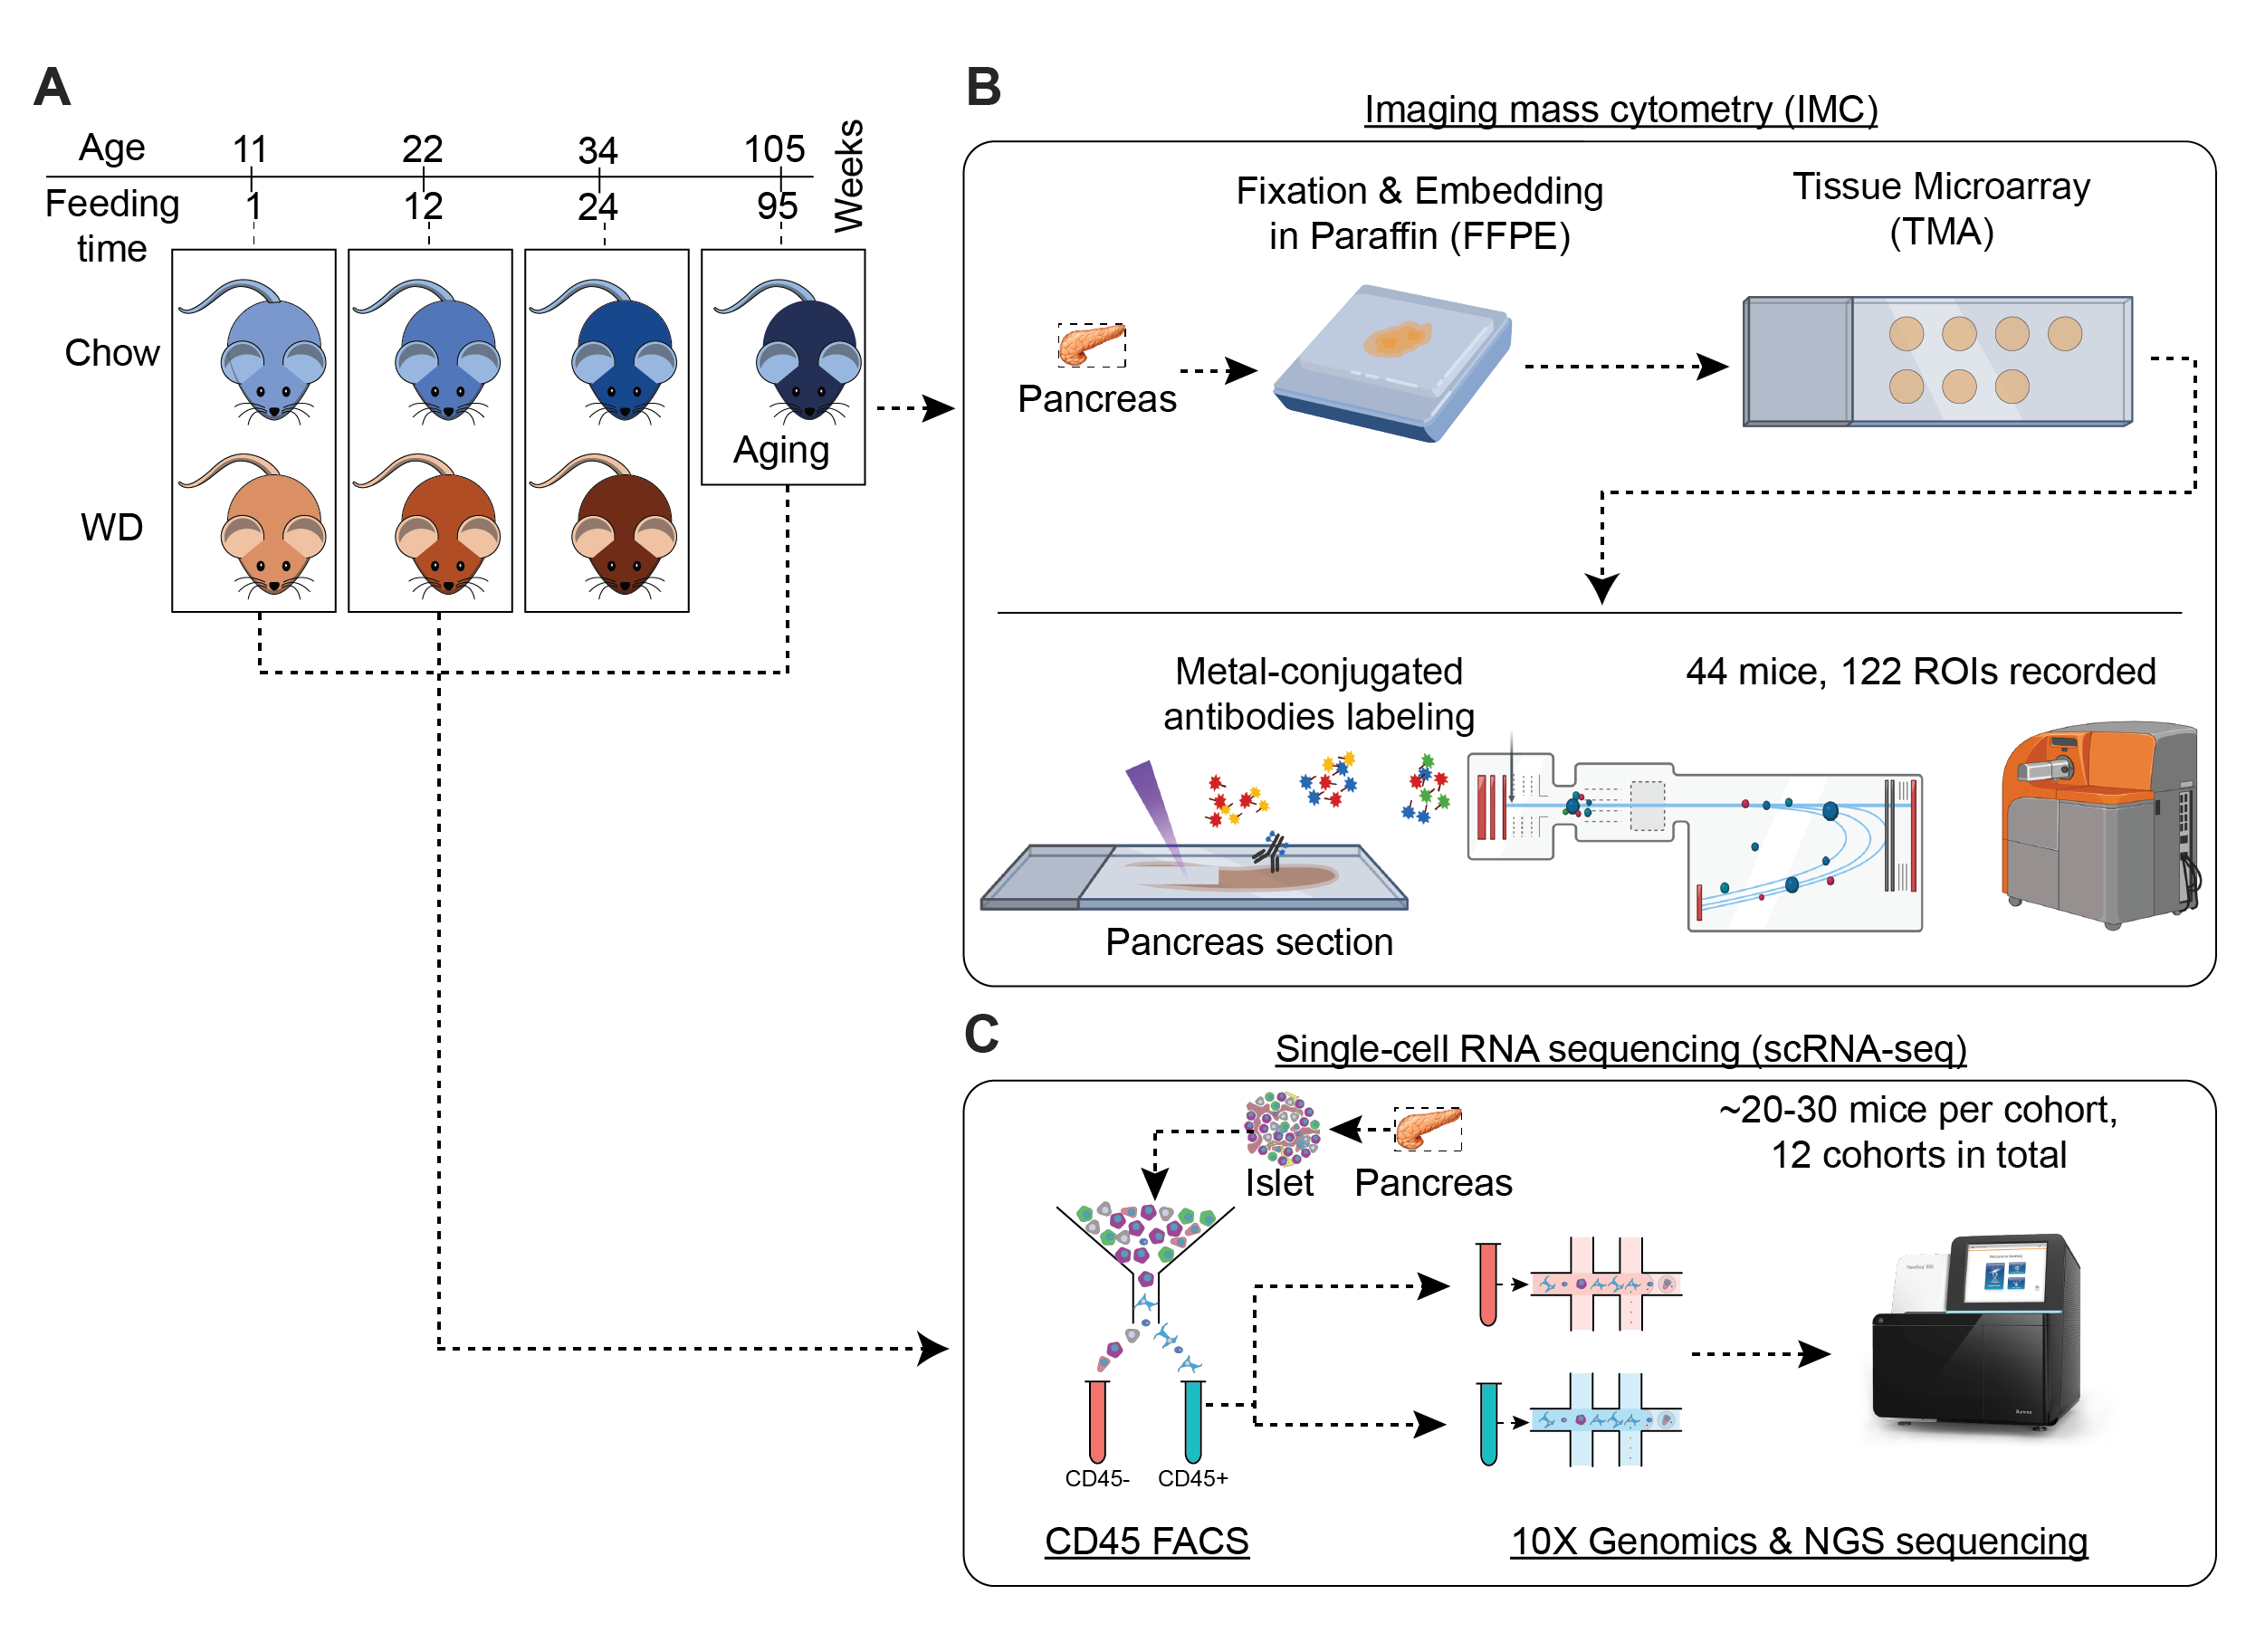
\includegraphics[width=15cm]{Chapter4/Fig/F2-1-01.png}
\caption[Experimental design to study \glsentryshort{wd}-induced obesity and aging]{\textbf{Experimental design to characterize changes in pancreatic immune cells during \gls{wd}-induced obesity and aging.} This illustration outlines the methodology where pancreas samples were harvested from at-least four mice at three post-\gls{wd} feeding time-points (W1, W12 and W24), alongside samples from age-matched, chow-fed mice and \textasciitilde2-year-old mice. These samples underwent \gls{imc} analysis using an established panel of markers targeting several immune populations, islet $\beta$-cells and endothelial cells \textbf{(\autoref{tab:app_imc_panel})}. For \gls{scr} analysis, islets from ten cohorts across early (W1) and mid-term (W12) \gls{wd} stages and two chow-fed aging cohorts, were isolated. \textasciitilde20-30 mice contributed to each cohort. Post-isolation, islet cells were \glsentryshort{facs}-sorted into immune (CD45\textsuperscript{+}) and non-immune (CD45\textsuperscript{-}) groups and processed via the 10x Genomics v3 protocol, and sequenced.}
\label{fig:chp2_experimental_design}
\end{figure}

 to \gls{wd} or a control chow diet feeding for 1 week (W1), 12 weeks (W12), or 24 weeks (W24). In addition, we incorporated samples from a cohort of \textasciitilde2-year-old to contrast between metabolic and aging-associated stress. This allowed us to compare the spatial organization of immune cells under these conditions. To complement the \gls{imc} spatial data with molecular profiles, we performed \gls{scr} on isolated CD45\textsuperscript{+} immune cells and CD45\textsuperscript{-} non-immune populations from the pancreatic islets \textbf{(}see \hyperref[subsec:met_chp2_scrdata]{\textbf{Methods}}\textbf{)}. In the \gls{scr} analysis, our objective was to detect initial molecular alterations triggered by the \gls{wd} feeding, focusing on samples collected at W1 and W12 feeding time-points \textbf{(\autoref{fig:chp2_experimental_design})}. Additionally, we also included samples from \textasciitilde2-year-old mice in order to gain further insights regarding the aging-associated inflammatory processes that trigger \gls{t2d}.  %(\textbf{Fig.\ref{fig:wdaging_experimental_design}}).


%\clearpage
\section[Unraveling complex cellular heterogeneity within the pancreatic tissue and islets]{Unraveling complex cellular heterogeneity within the\\pancreatic tissue and islets}
\label{sec:chp2_imc_scrna}

\subsubsection{\large \gls{imc} data analysis}
\label{sec_chp2_imc1}

In the \gls{imc} analysis, pancreatic tissue sections from at least 4 mice for each feeding groups and time-points were included (in total, seven experimental conditions). In total, at least 10 \glspl{roi} were sampled for each of the seven experimental conditions, and 78 \glspl{roi} were used altogether to create 17 \glspl{tma}, each containing \glspl{roi} from different experimental conditions and time-points. \glspl{tma} were then subjected to comprehensive \gls{imc} analysis of 25 selected immune cell marker proteins \textbf{(\autoref{tab:app_imc_panel};} see \hyperref[subsec:met_chp2_imcdata]{\textbf{Methods}}\textbf{)}. Additionally, we used INS, \glsentryshort{glp1}R and NKX6-1 as markers of pancreatic islets. Using a comprehensive, standardized cell segmentation workflow, we achieved single-cell resolution of our  analysis \textbf{(\autoref{fig:app_imc_segmentation};} see \hyperref[subsec:met_chp2_imcdata]{\textbf{Methods}}\textbf{)}. We also included one \gls{roi} from a spleen sample in each individual \gls{tma}. This served as a cross-\gls{tma} reference for the batch correction of immune cell marker staining intensity channels across all \glspl{tma} \textbf{(\autoref{fig:app_imc_anchorbcell} A)}.\\


\begin{figure}[t]
\centering
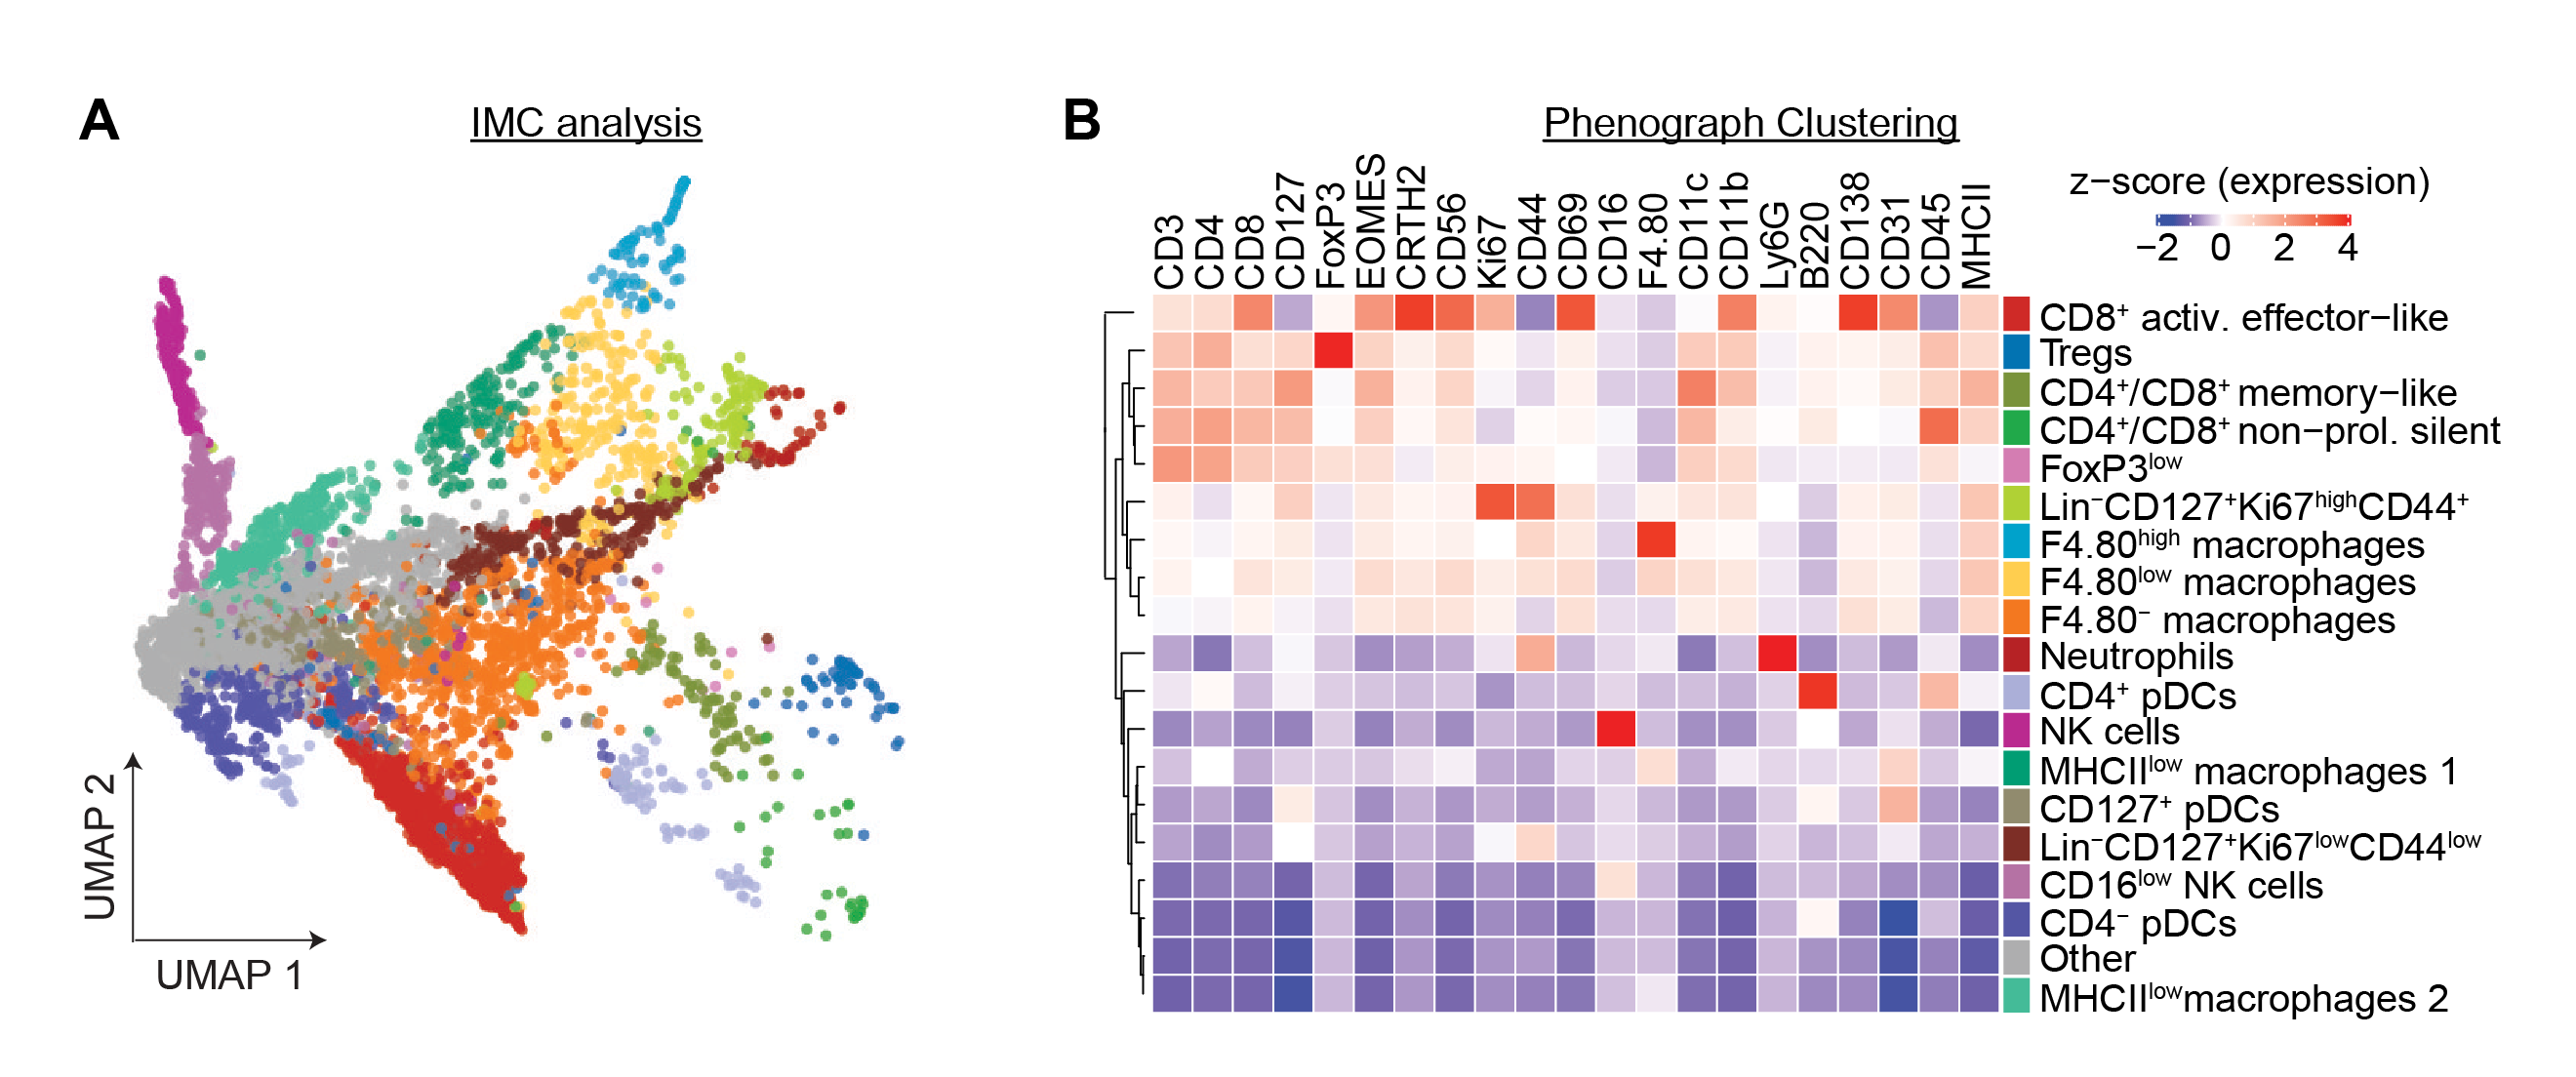
\includegraphics[width=\linewidth]{Chapter4/Fig/F2-2-01.png}
\caption[Characterization of immune cell populations with \glsentryshort{imc}]{\textbf{Characterization of immune cell populations with \gls{imc}.} \textbf{(A)} \gls{umap} embedding of the CD45\textsuperscript{+}CD19\textsuperscript{-} immune cell populations identified by \gls{imc} analysis. \textbf{(B)}  Heatmap depicting the Phenograph clustering and transformed \textit{z-scores} of protein expression for the immune cell marker channels. The identities of the sub-populations were defined based on the relative expression levels of these marker proteins. \textit{This data and figure were originally generated by Dr. Matthias Barone and reused here with permission.}}
\label{fig:chp2_imc_umap}
\end{figure}

\par The pancreatic islets were identified using the INS, NKX6-1 and \glsentryshort{glp1} channels, whereas the pancreatic lymph nodes were marked using B220, CD19, CD44 and CD45 channels \textbf{(\autoref{tab:app_imc_panel})}. Interestingly, CD19\textsuperscript{+} B-cells were nearly all localized within the pancreatic lymph nodes \textbf{(\autoref{fig:app_imc_anchorbcell} B,C)}, and were therefore not selected for subsequent analyses. Cluster analysis of the selected CD45\textsuperscript{+}CD19\textsuperscript{-} immune cells using Phenograph enabled us to identify a wide variety of immune cell populations, including different CD3 expressing T-cell sub-populations, such as EOMES\textsuperscript{+}CD56\textsuperscript{+}KI67\textsuperscript{+}CD69\textsuperscript{+} activated effector-like CD8\textsuperscript{+} cells, FOXP3\textsuperscript{+} \gls{treg}, CD127\textsuperscript{\textit{high}}CD4\textsuperscript{+}/CD8\textsuperscript{+} memory-like cells, KI67\textsuperscript{-}CD4\textsuperscript{+}/CD8\textsuperscript{+} non-proliferative silent cells, and FOXP3\textsuperscript{\textit{low}}CD4\textsuperscript{+} T-cells, differently activated macrophage sub-populations such as F4/80\textsuperscript{-}CD11c\textsuperscript{\textit{high}}, F4/80\textsuperscript{\textit{low}}CD11c\textsuperscript{\textit{high}}, F4/80\textsuperscript{\textit{high}}CD11c\textsuperscript{\textit{low}}, and two \glsentrylong{mhc2} low (\glsentryshort{mhc2}\textsuperscript{\textit{low}}) sub-populations, three types of B220 expressing plasmacytoid dendritic-like cells (\glsentryshort{pdc}) - CD4\textsuperscript{+}, CD4\textsuperscript{-}, and CD127\textsuperscript{+}, Ly6G\textsuperscript{+} neutrophils, CD16\textsuperscript{\textit{high}} natural killer (\glsentryshort{nk}) cells, and Lin\textsuperscript{-}CD127\textsuperscript{+} innate lymphoid-like cells (\glsentryshort{ilc}s) \textbf{(\autoref{fig:chp2_imc_umap})}. Thus, our \gls{imc} analysis facilitated the identification and characterization of diverse immune cell populations within the pancreatic tissue.

\subsubsection{\large \gls{scr} data analysis}
\label{sec_chp2_scrna1}
Similarly, we applied a robust \gls{qc} and data integration pipeline to our \gls{scr} data \textbf{(\autoref{fig:app_scrna_qc} A-C}, see \hyperref[subsec:met_chp2_scrdataprocess]{\textbf{Methods}}\textbf{)}, yielding 125,372 high-quality single-cell transcriptomic profiles of CD45\textsuperscript{+} immune cells and CD45\textsuperscript{-} non-immune cells, annotated based on the expression of CD45 gene, \textit{Ptprc} \textbf{(\autoref{fig:chp2_fullscRNA} A)}. The immune and the non-immune populations were further analyzed separately by assessing the respective cells, performing additional \gls{qc} steps when necessary and re-integrating the subsets to allow for more granular characterization of the immune and non-immune populations within the pancreatic islets \textbf{(}see \hyperref[subsubsec:met_chp2_immuneendo]{\textbf{Methods}}\textbf{)}.

\begin{figure}[H]
\centering
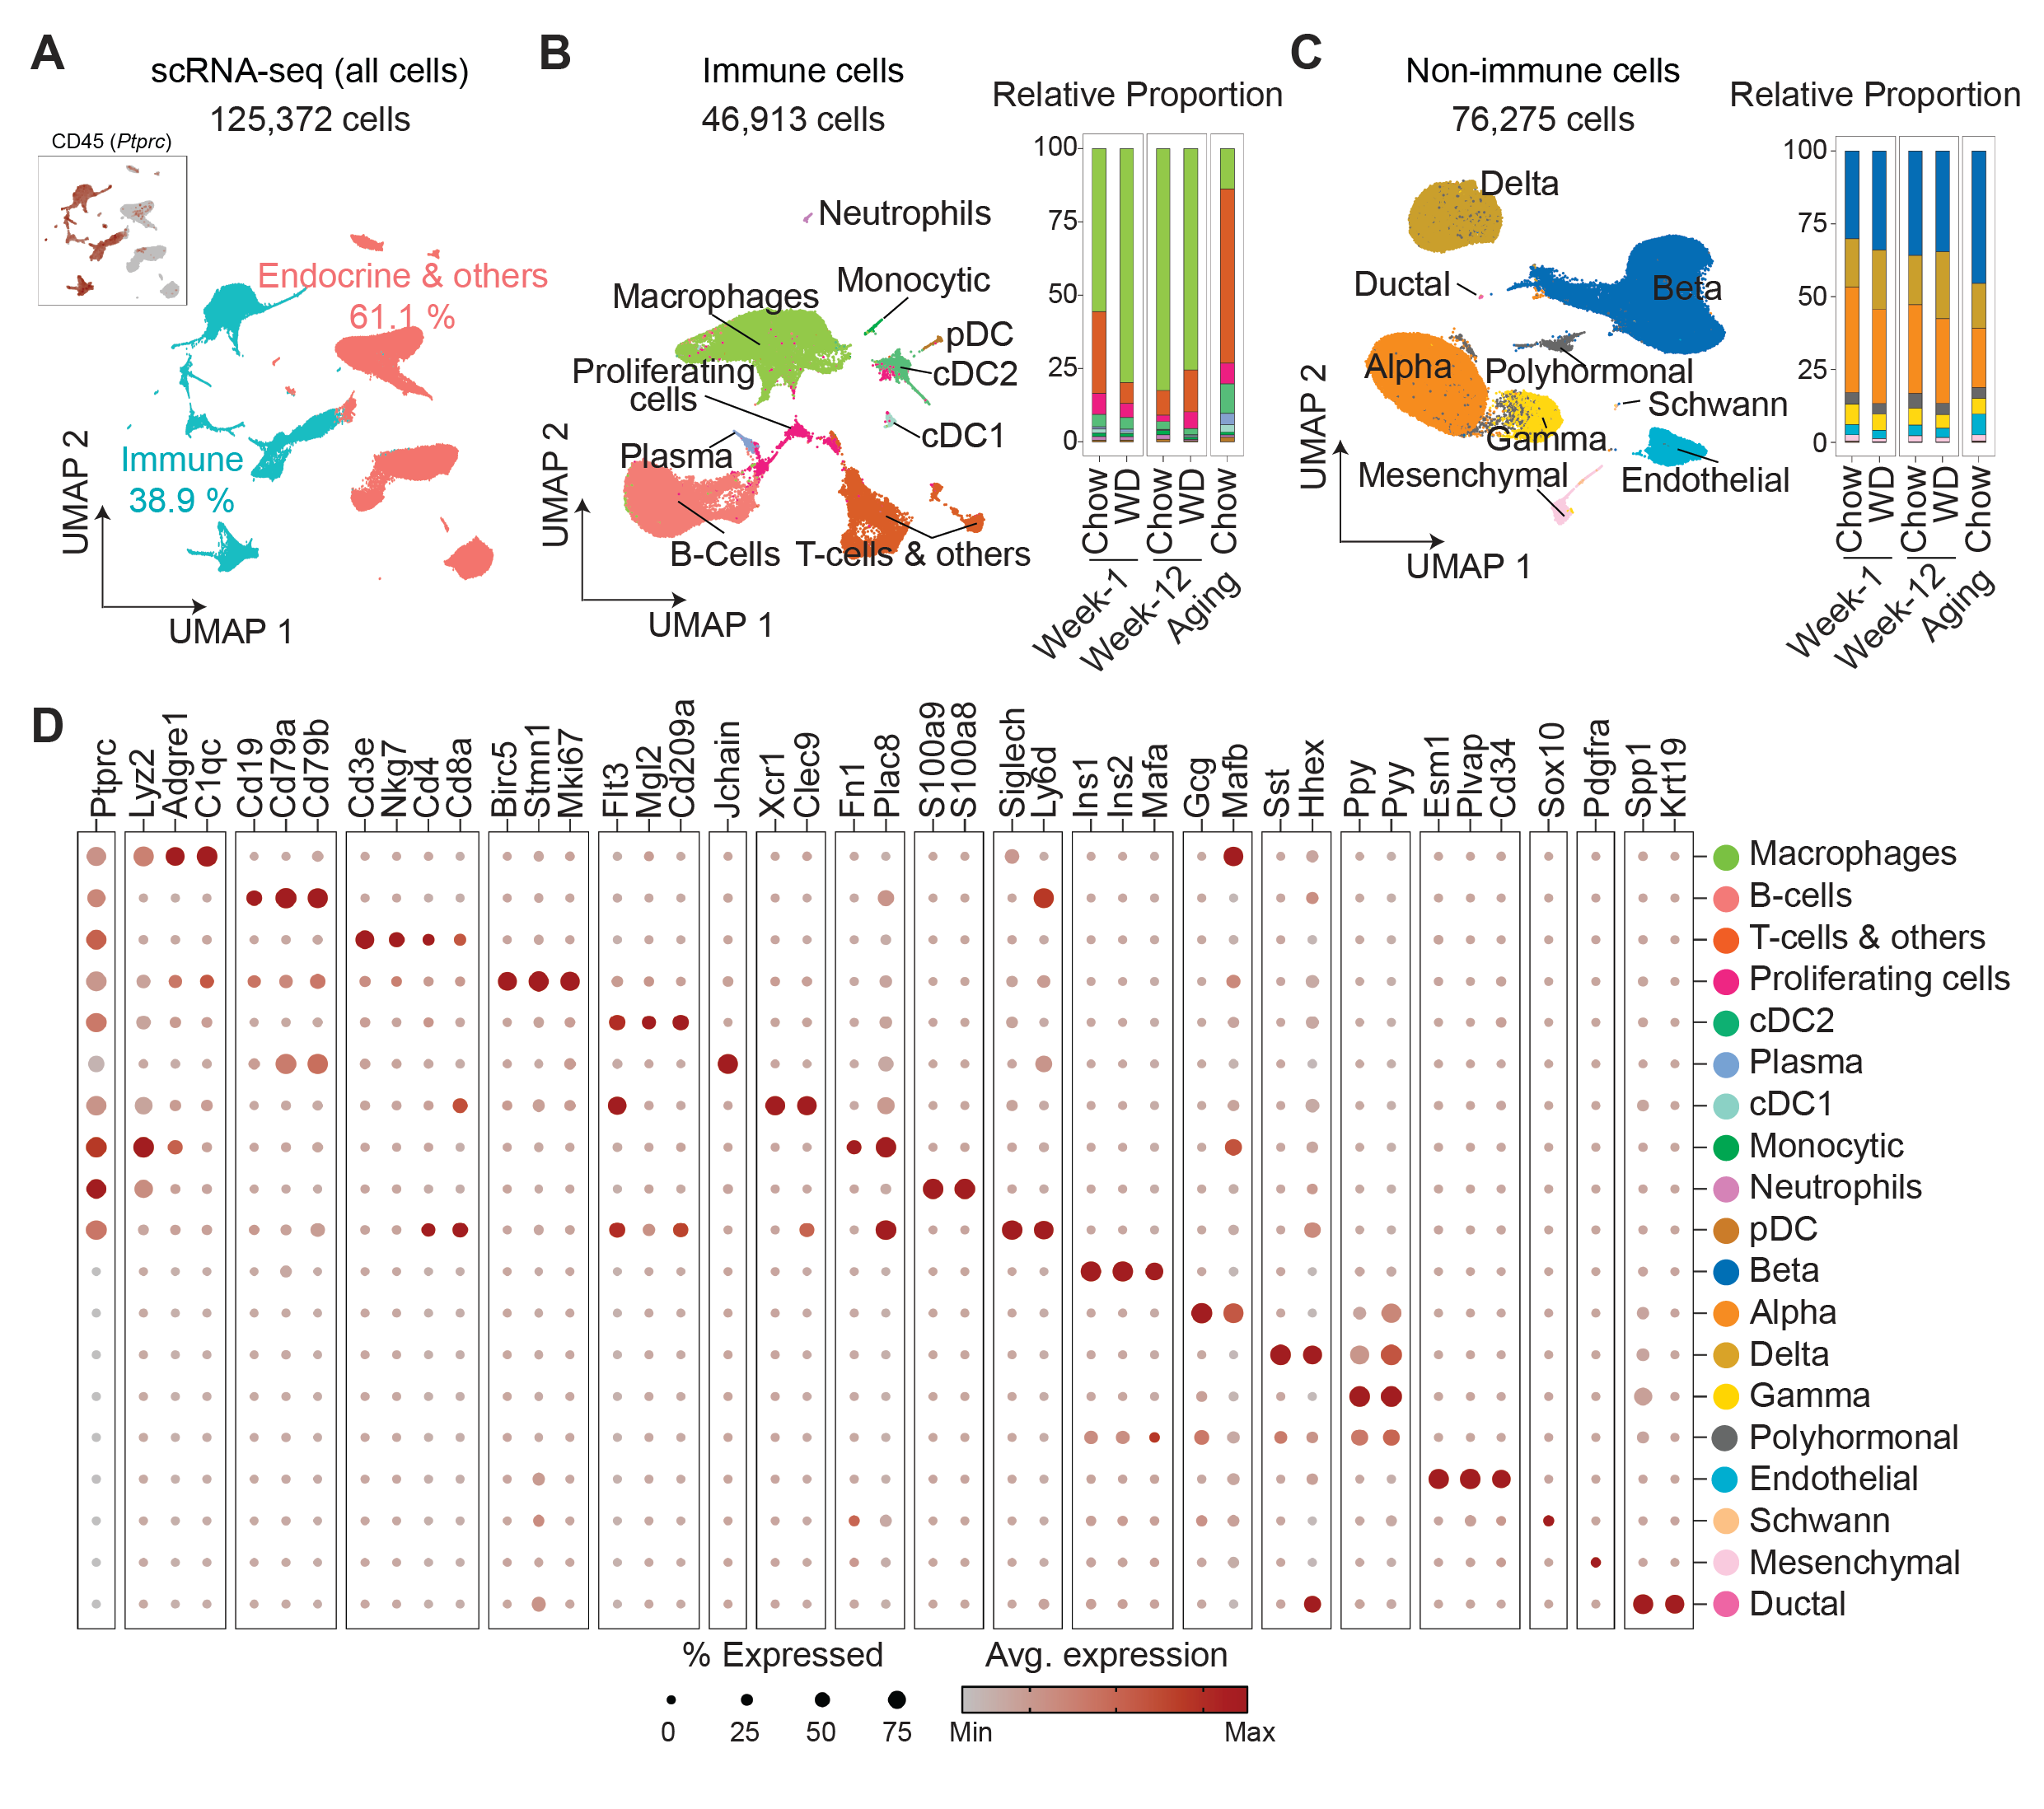
\includegraphics[width=\linewidth]{Chapter4/Fig/F2-3-01.png}
\caption[Revealing the complex heterogeneity of pancreatic islets with \glsentryshort{scr}]{\textbf{Revealing the complex heterogeneity of pancreatic islets with \gls{scr}} \textbf{(A)} \gls{umap} embedding of the integrated data consisting of 125,372 single cells across twelve cohorts. The immune cells were annotated based on the expression of CD45 (\textit{Ptprc}) and the remaining cells were labelled as `Endocrine \& others'. Values indicate the overall proportion of each annotated population. \textbf{(B)} \gls{umap} embedding of the immune cell population, following additional \gls{qc} and subsequent re-integration. Cluster identities were defined based on the expression of known immune markers. \textbf{(C)} The proportion of each annotated immune cell sub-populations computed as a percentage of total immune cells in every experimental group. The cells from different biological replicate cohorts were pooled together. B-cells were excluded from calculation and are therefore not represented. \textbf{(D)} \gls{umap} embedding of the `Endocrine \& others' cell populations, following additional \gls{qc} and subsequent re-integration. Cluster identities were defined based on the expression of known gene markers. \textbf{(E)} The proportion of each annotated endocrine, exocrine and other cell populations computed as a percentage of total non-immune cells in every experimental group. The cells from different biological replicate cohorts were pooled together. \textbf{(F)} Combined dot plot showing hallmark marker genes for all annotated cell types in \textbf{(B)} and \textbf{(D)}. The color of the dots represent the scaled average expression of the genes and the size of the dots correspond to the percentage of cells expressing the gene.}
\label{fig:chp2_fullscRNA}
\end{figure}

\par Our approach, focusing on CD45 enrichment \textbf{(\autoref{fig:chp2_experimental_design})}, allowed us to profile a total of 46,913 islet-associated immune cells, which currently represents the most comprehensive immune cell map available for mouse islets \textbf{(\autoref{fig:chp2_fullscRNA} B; \autoref{fig:app_scrna_qc} A,C)}. Utilizing the expression of known markers \textbf{(\autoref{fig:chp2_fullscRNA} F)}, we confirmed the presence of macrophages (marked by \textit{Lyz2, Adgre1, C1qc}), monocytes (identified by \textit{Fn1, Plac8}), neutrophils (\textit{S100a9, S100a8}), dendritic cells (indicated by \textit{Xcr1, Flt3, Siglech}), and a variety of lymphocytes such as T-cells (expressing \textit{Cd3e, Cd4, Cd8a}), B-cells (transcribing \textit{Cd19, Cd79a} and \textit{Cd79b}), and plasma cells (marked by \textit{Jchain}). The macrophages represented the major immune population within the islets of adult mice (W1 and W12) \textbf{(\autoref{fig:chp2_fullscRNA} C)}. However, the proportion of T-cells was highest in the cohort of older mice \textbf{(\autoref{fig:chp2_fullscRNA} C)}, which is in line with the observation of significant accumulation of T-cells in aging mice \textbf{\cite{denroche_t_2021}}. Of note, B-cells were also excluded in downstream analyses of the single-cell data, as they were primarily associated with pancreatic lymph nodes in the \gls{imc} analysis \textbf{(\autoref{fig:app_imc_anchorbcell} B,C)} and their proportion across the single-cell cohorts was also inconsistent \textbf{(\autoref{fig:app_scrna_qc} A)}. The remaining immune populations represented a minor fraction of the total islet-associated immune cells across all cohorts in the single-cell data \textbf{(\autoref{fig:chp2_fullscRNA} C)}.\\% Our \gls{scr} analysis further enabled the investigation of islet-associated immune cells at a resolution that is significantly superior to that achievable with \gls{ihc}.\\

\par We also profiled 76,275 islet-associated CD45\textsuperscript{-} cells from the same cohort of animals, which consisted of pancreatic endocrine and exocrine cells, endothelial cells, mesenchymal cells and schwann cells, based on well-established hallmark gene expression patterns \textbf{(\autoref{fig:chp2_fullscRNA} D,F; \autoref{fig:app_scrna_qc} B,C)} \textbf{\cite{van_gurp_generation_2022}}. We annotated the endocrine populations as Alpha ($\alpha$) - \textit{Gcg, Mafb}; Beta ($\beta$) -\textit{Ins1, Ins2, Mafa}; Delta ($\delta$) - \textit{Sst, Hhex} cells and Gamma ($\gamma$) - \textit{Ppy, Pyy}, also known as \gls{pp}-cells, based on the expression of primary islet hormones and \glspl{tf} \textbf{(\autoref{fig:chp2_fullscRNA} D,F)}. $\beta$-cells constituted the major fraction of endocrine cells (\textasciitilde37\%), followed by $\alpha$-cells (\textasciitilde30\%), $\delta$-cells (\textasciitilde19\%) and \gls{pp}-cells (\textasciitilde6\%) \textbf{(\autoref{fig:chp2_fullscRNA} E)}. In line with previous studies, the proportion of $\beta$-cells in the chow diet-fed aging cohort was higher compared to the all the non-aging (W1 and W12) cohorts \textbf{(\autoref{fig:chp2_fullscRNA} E)} \textbf{\cite{tuduri_pancreatic_2022}}. Consistent with methodologies employed in published reports, endocrine cells expressing more than one hormone marker were classified as polyhormonal cells and accounted for \textasciitilde4\% of the data \textbf{(\autoref{fig:app_scrna_qc} D,E)} \textbf{\cite{sachs_targeted_2020, perez-frances_pancreatic_2021}}. The other endocrine populations, as well as the exocrine cells, did not show any shifts in their cellular proportions in response to metabolic stress or aging. The mesenchymal (2\%), schwann (1\%), ductal (1\%) and endothelial (5\%) cells together made up less that 10\% of the single-cell data \textbf{(\autoref{fig:chp2_fullscRNA} E)}, thereby reflecting the efficiency of the islet isolation step during sample preparation.\\

\par Thus, the CD45\textsuperscript{+} enrichment combined with single-cell transcriptomics enabled a detailed characterization of the immune landscape within pancreatic islets. Further, integrating with \gls{imc}, we have constructed a comprehensive representation of the immune cells within the mouse pancreas, encompassing both their spatial distribution and molecular characteristics. 

%\clearpage

\section[Metabolic stress accelerates aging-induced accumulation of inflammatory F4/80\textsuperscript{\textit{low}} macrophages]{Metabolic stress accelerates aging-induced accumulation \\of inflammatory F4/80\textsuperscript{\textit{low}} macrophages}
\label{sec:imc_acceleration}

We subsequently investigated whether immune cell populations within the pancreas expanded in response to \gls{wd}-feeding or aging. Using \gls{imc}, we assessed the density of each immune cell population and detected significant changes in the macrophage abundance across metabolic stress and aging \textbf{(\autoref{tab:app_imc_macrophages})}. This affected the three macrophage sub-populations expressing various levels of CD11c and F4/80: F4/80\textsuperscript{\textit{high}}, F4/80\textsuperscript{\textit{low}}, and F4/80\textsuperscript{\textit{-}} \textbf{(\autoref{fig:chp2_imc_umap} B, \autoref{fig:chp2_imc_macrophages1} A)}. Our analysis primarily centered on two major aspects of sub-population dynamics: 
\begin{enumerate}
    \item The relative enrichment of these cells within the entire pancreas and
    \item The accumulation of these immune cells in specific regions, namely the pancreatic islets and the peri-islet areas.
\end{enumerate}

To address the second aspect, we identified the islet regions based on INS, NKX6-1 and \glsentryshort{glp1} channels. To evaluate both, the expansion of islet-resident immune cells and the recruitment of immune cells to the periphery of the islet, we defined a peri-islet region that extended 70\textmu m beyond the boundary of the identified islets \textbf{(\autoref{fig:chp2_imc_macrophages1} B)}. Our --


\begin{figure}[H]
    \centering
    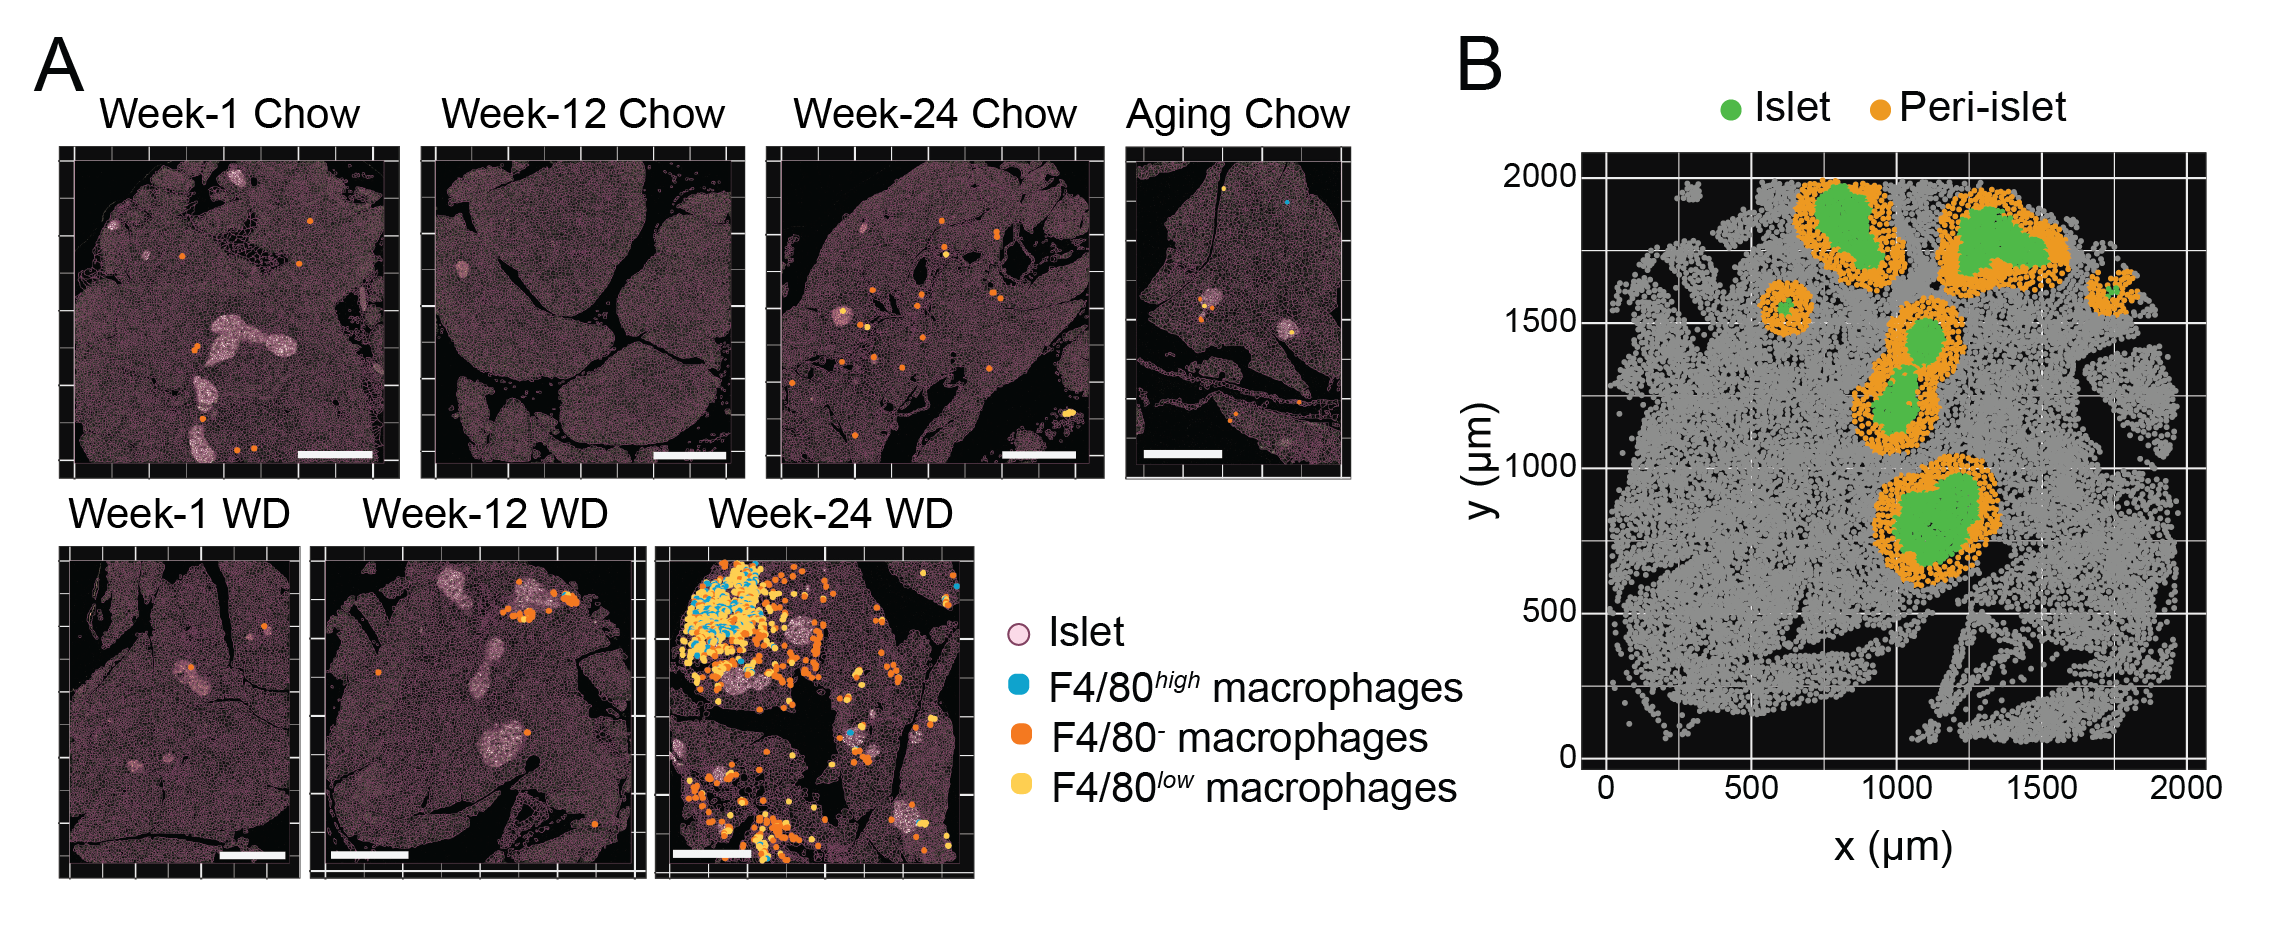
\includegraphics[width=\linewidth]{Chapter4/Fig/F2-9-01.png}
    \caption[Mapping macrophages within pancreatic tissue]{\textbf{Mapping macrophages within pancreatic tissue.} \textbf{(A)} Representative \glspl{roi} showing the three macrophage sub-populations expressing different levels of CD11c and F4/80: F4/80\textsuperscript{\textit{high}}, F4/80\textsuperscript{\textit{low}}, and F4/80\textsuperscript{\textit{-}} in the pancreas. Pancreatic islet regions are marked by INS channel. Scale bar 500 \textmu m. \textbf{(B)} Representative image illustrating a pancreatic islet (green) enclosed by peri-islet region (yellow) encompassing the area extending from the islet boundary up to 70\textmu m away. \textit{This data and figure were originally generated by Dr. Matthias Barone and reused here with permission.}}
    \label{fig:chp2_imc_macrophages1}
\end{figure}
 
-- observations indicated that most immune cell populations in the pancreas remained stable under metabolic stress or progressive aging \textbf{(\autoref{fig:chp2_imc_macrophages2} A, \autoref{fig:app_imc_macrophages})}. However, there was a notable increase in F4/80\textsuperscript{\textit{low}} macrophages across the entire pancreas \textbf{(\autoref{fig:chp2_imc_macrophages2} A}, middle\textbf{; \autoref{fig:app_imc_macrophages} B,E)}. These cells also accumulated within the islets and their adjacent areas. Due to the higher variability in \gls{wd} feeding, this became only significant in the aging condition \textbf{(\autoref{fig:chp2_imc_macrophages2} B}, middle\textbf{)}. Overnutrition also caused a mild elevation in F4/80\textsuperscript{\textit{-}} macrophages throughout the pancreas \textbf{(\autoref{fig:chp2_imc_macrophages2} A}, right\textbf{; \autoref{fig:app_imc_macrophages} C,F)}, whereas F4/80\textsuperscript{\textit{high}} macrophages stayed constant, irrespective of the conditions \textbf{(\autoref{fig:chp2_imc_macrophages2} A}, left\textbf{; \autoref{fig:app_imc_macrophages} A,D)}. Additionally, neither F4/80\textsuperscript{\textit{high}} \textbf{(\autoref{fig:chp2_imc_macrophages2} B}, left\textbf{)}  and F4/80\textsuperscript{\textit{-}} \textbf{(\autoref{fig:chp2_imc_macrophages2} B}, right\textbf{)} macrophages moved closer to the islet region under either of the metabolic stresses.\\

\begin{SCfigure}[][h]
  \centering
  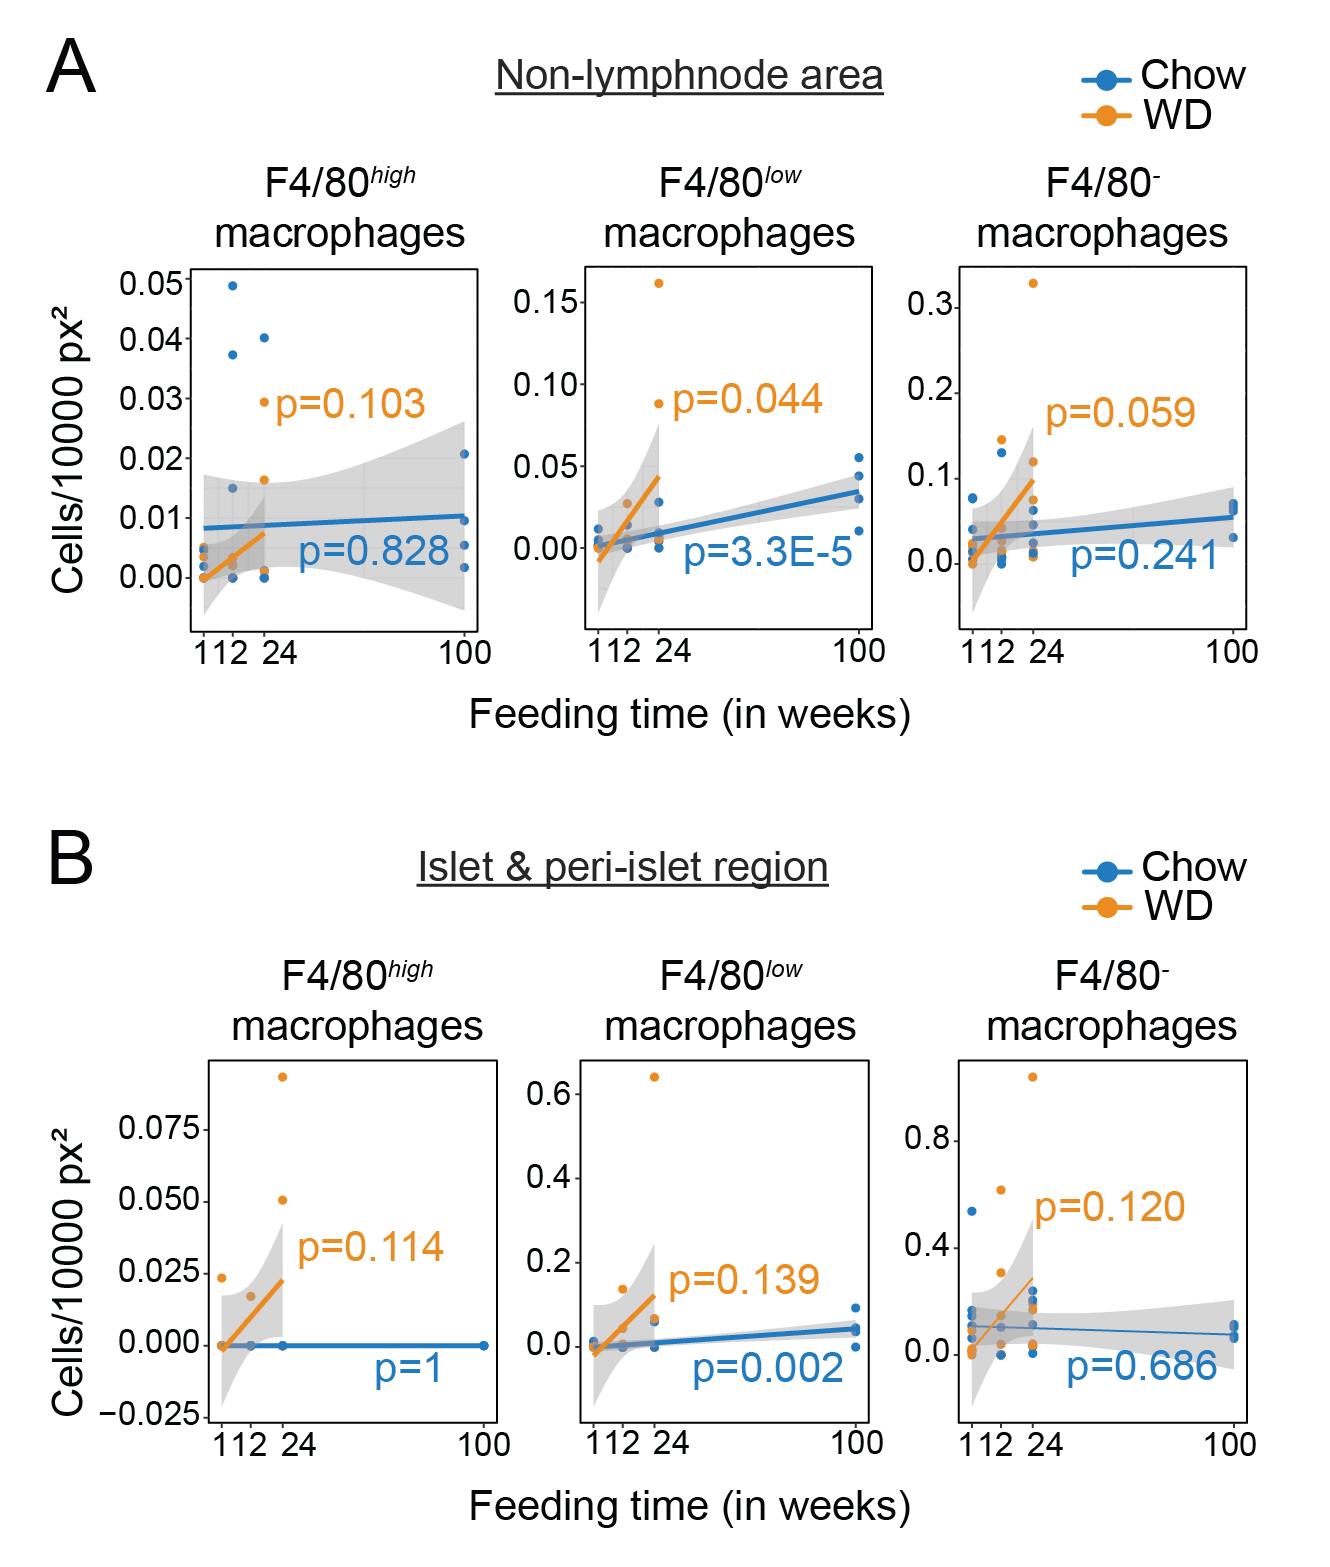
\includegraphics[width=0.5\linewidth]{Chapter4/Fig/F2-9-02.png}
  \vspace{-10pt}
  \caption[Accumulation of inflammatory macrophages within the pancreas]{\textbf{\gls{wd} accelerates aging-induced accumulation of inflammatory F4/80\textsuperscript{\textit{low}} macrophages}.\textbf{(A) - (B)} Scatter plots depicting the cell counts of F4/80\textsuperscript{\textit{high}}, F4/80\textsuperscript{\textit{low}} and F4/80\textsuperscript{\textit{-}} macrophages per area of the pancreas (excluding lymph nodes) \textbf{(A)} and per area within the pancreatic islets and peri-islet regions \textbf{(B)}  across all experimental conditions. Linear regression fits representing the cell count per area trends over time are plotted as solid lines. The 95\% confidence intervals for each linear regression are highlighted in grey. p-values for regressions were determined using t-tests. \textit{This data and figure were originally generated by Dr. Matthias Barone and reused here with permission.}}
  \label{fig:chp2_imc_macrophages2}

\end{SCfigure}

\vspace{20pt}

\par In summary, our analysis revealed a \gls{wd} feeding accelerated the accumulation of F4/80\textsuperscript{\textit{low}} macrophages within the pancreas, an effect that occurs naturally during aging under chow diet. Interestingly, conditions of overnutrition also promote the accumulation of another inflammatory macrophage sub-population - F4/80\textsuperscript{-} macrophages, which did not increase with aging.%  -mediated acceleration of the accumulation of the F4/80\textsuperscript{\textit{low}} macrophages within the pancreas and peri-islet regions, which under chow diet only happens later in life. Metabolic stress also favored accumulation of another inflammatory CD11c\textsuperscript{\textit{high}} expressing F4/80\textsuperscript{\textit{-}} macrophages, which was not observed in aging.

% \begin{figure}
% \floatbox[{\capbeside\thisfloatsetup{capbesideposition={right,top},capbesidewidth=4cm}}]{figure}[\FBwidth]
% {\caption{A test figure with its caption side by side}\label{fig:test}}
% {\includegraphics[width=5cm]{}}
% \end{figure}

% \begin{figure}
%     \floatbox[{\capbeside\thisfloatsetup{capbesideposition={right,top},capbesidewidth=4cm}}]{figure}[\FBwidth]
    
%     {\caption{Caption}\label{fig:enter-label}}
%     {\includegraphics{}}
    
% \end{figure}


% \mysidecaption{0.4}{%
% \captionof{figure}[Linking macrophage sub-populations between scRNA-seq and IMC analyses]{\textbf{.} \textbf{(A)} Violin plots depicting the normalized expression levels of selected markers with corresponding channels in the IMC panel. The top plots compare these levels across various macrophage sub-populations, and the bottom plots display their expression in the Macs-3 population under different experimental conditions. \textbf{(B)}Heatmap showing z-scored expression of selected IMC channgels across the four macrophage sub-populations identified in the IMC analysis. Corresponding macrophage sub-populations from scRNA-seq analysis are indicated in parantheses. \textbf{(C)} Violin plots of \textit{arcsinh} transformed expression of selected IMC channels in the F4/80\textsuperscript{\textit{low}} macrophage sub-population from the IMC analysis across experimental conditions. * p<0.05, ** p<0.01, *** p<0.001 and **** p<0.0001. p-values were calculated using the Wilcoxon rank-sum test with Bonferroni correction.}%
% }
% {%
% \begin{figure}
%    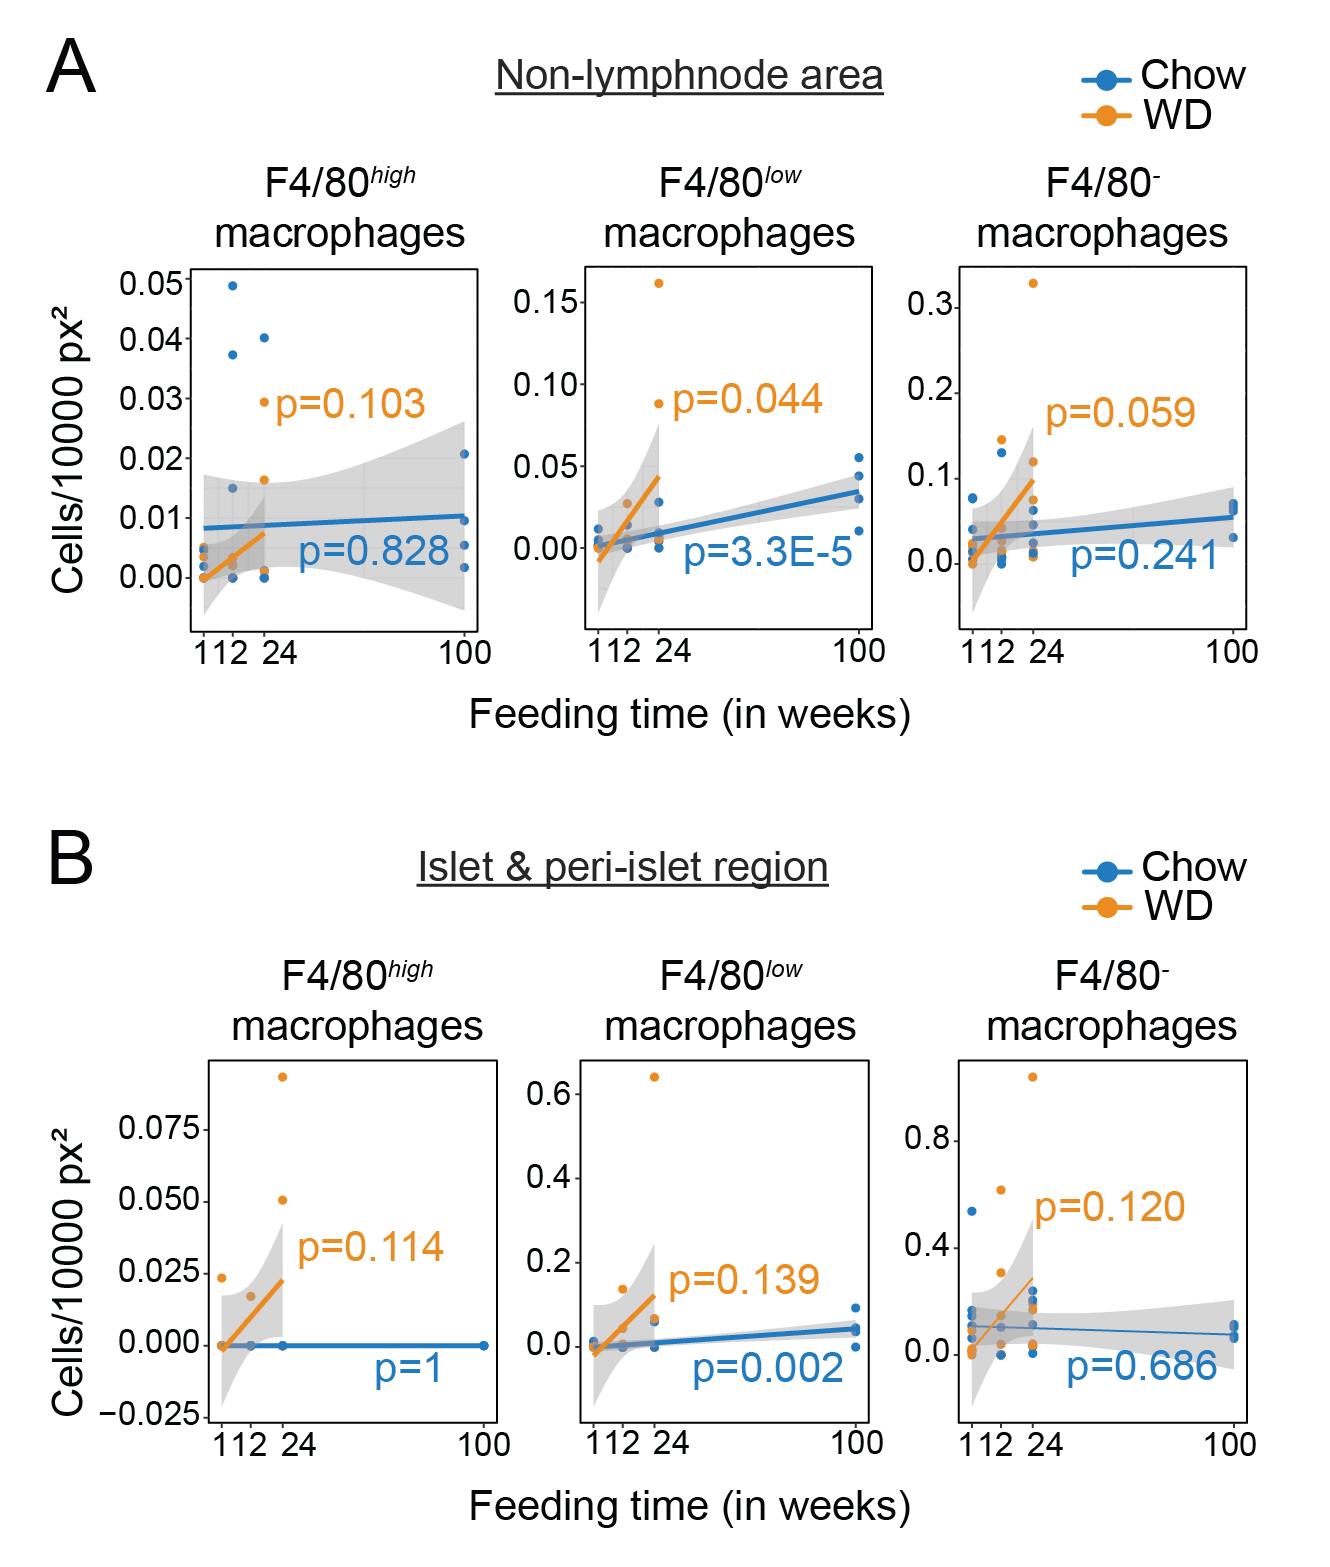
\includegraphics[width=9cm,height=11cm,keepaspectratio]{Chapter4/Fig/F2-9-02.png}%
%    \label{fig:chp2_imc_macrophages2}
% \end{figure}
% }[t]%



% \begin{figure}[b]
%     \centering
%     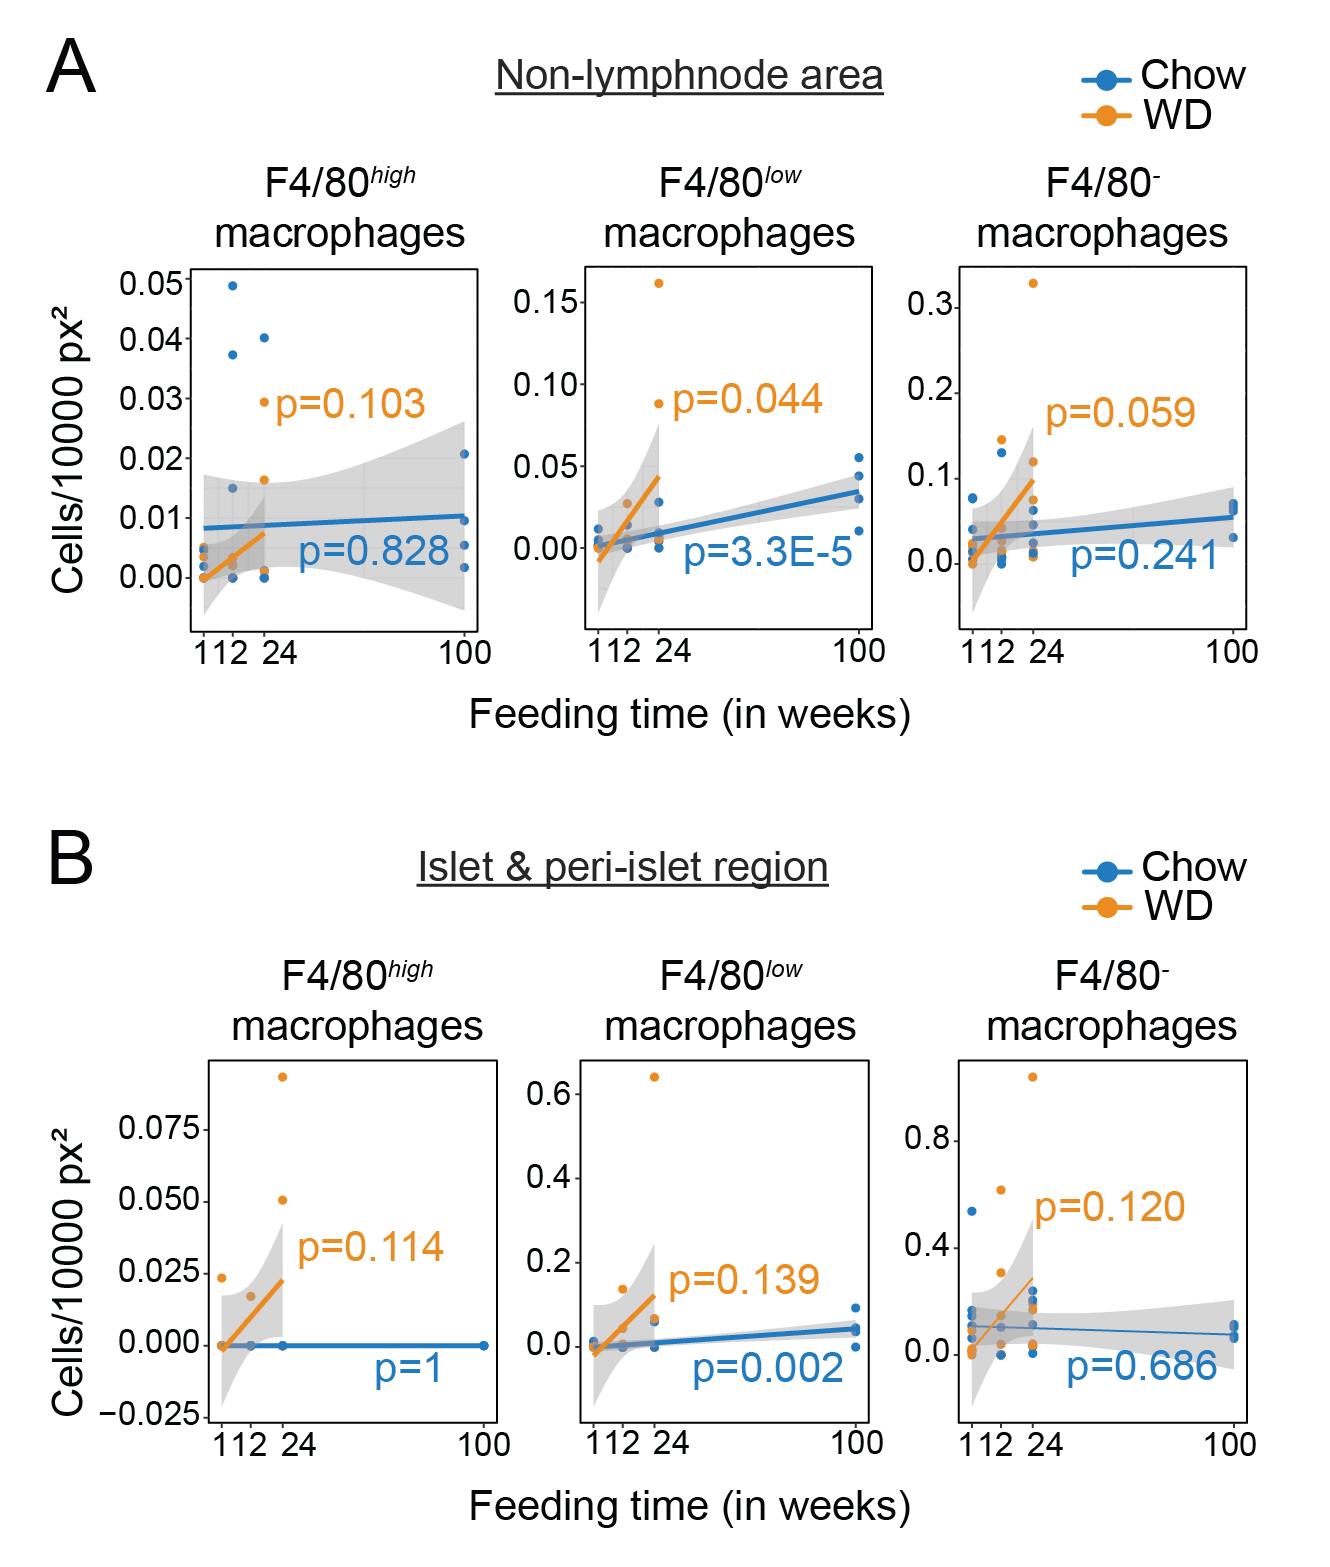
\includegraphics[width=\linewidth]{Chapter4/Fig/F2-9-02.png}
%     \caption[Accumulation of inflammatory macrophages within the pancreas]{\textbf{\gls{wd} accelerates aging-induced accumulation of inflammatory F4/80\textsuperscript{\textit{low}} macrophages.} \textbf{(A) - (B)} Scatter plots showing the cell counts of F4/80\textsuperscript{\textit{high}}, F4/80\textsuperscript{\textit{low}} and F4/80\textsuperscript{\textit{-}} macrophages per area of the pancreas (excluding lymph nodes) \textbf{(A)} and per area within the pancreatic islets and peri-islet regions \textbf{(B)}  across four time-points and two feeding conditions. Linear regression fits representing the cell count per area trends over time are plotted as solid lines. The 95\% confidence intervals for each linear regression are highlighted in grey. p-values for regressions were determined using t-tests. \textit{This data and figure were originally generated by Dr. Matthias Barone and reused here with permission.}}
%     \label{fig:chp2_imc_macrophages2}
% \end{figure}


\clearpage

\section[\glsentryshort{ifn}-activated macrophages are enriched in the islets in response to metabolic- and aging-induced stress]{Interferon-activated macrophages are enriched in the\\islets in response to metabolic- and aging-induced stress}
\label{sec:chp2_sc_macs}

% %\subsection{Characterization of islet-intrinsic macrophage sub-populations\\using scRNA-seq\\}
% Macrophages are the only resident myeloid cells found in islets of all mouse strains, under normal conditions \textbf{\cite{zakharov_single-cell_2020}}. The presence of islet-resident macrophages is essential for the normal islet development, $\beta$-cell regeneration and regulation of insulin secretion \textbf{\cite{ying_expansion_2019}}. In diet-induced islet inflammation, islet-resident macrophages have been shown to impair $\beta$-cell insulin secretion while also promoting adaptive $\beta$-cell proliferation % via PDGFR signaling. This suggests that macrophages within islets are heterogeneous in function and that diet could alter the abundance of specific macrophage subsets in pancreatic islets.

While the role of islet macrophages in perpetuating islet inflammation is known, discrepancies exists around nature of islet macrophages in insulin-resistant and \gls{t2d} models. We therefore performed detailed single-cell characterization of the islet-associated macrophages identified in our \gls{scr} data. 

\subsubsection{\large Annotating islet-intrinsic macrophages using gene expression}
 
\par To characterize the islet-associated macrophages, we extracted the macrophages from the CD45\textsuperscript{+} immmune single-cell dataset \textbf{(\autoref{fig:chp2_fullscRNA} B)} and performed sub-clustering analysis. We identified a total of five macrophage sub-populations which included a homeostatic, non-activated population (Macs-1), two activated populations, (Macs-2 and Macs-3), a proliferating population (Macs-4), and a phagocytic population (Macs-5) \textbf{(\autoref{fig:chp2_scrna_macrophages} A)}. Contrary to the homeostatic Macs-1, both Macs-2 and Macs-3 displayed a pro-inflammatory phenotype, characterized by type-2 and type-1 \gls{ifn} response gene signature respectively. The level of activation was more dramatic in Macs-3 than in Macs-2 \textbf{(\autoref{fig:chp2_scrna_macrophages} B,C; \autoref{tab:app_scrna_macrophages_markers})}. Intriguingly, the highest expression of \textit{Ifnb1} was observed in Macs-2, suggesting it as the likely initiator of the \gls{ifn} response \textbf{(\autoref{fig:app_scrna_macrophages_macs2_genes} A)}. Additionally, Macs-2 showed higher expression of genes downstream of \gls{tnf} and \gls{nfkb} when compared to Macs-1, a trait that was not present in Macs-3 \textbf{(\autoref{fig:chp2_scrna_macrophages} C)}. Macs-4 represented group of islet-macrophages expressing genes involved in cell-cycle pathways, and together with Macs-1, likely constitute the macrophages involved in islet homeostatic functions \textbf{(\autoref{fig:chp2_scrna_macrophages} B,C; \autoref{tab:app_scrna_macrophages_markers})}. This finding of islet macrophages with self-replicating capacity is consistent with a previous study \textbf{\cite{calderon_pancreas_2015}}. Finally, the gene expression signature of Macs-5 was associated with apoptotic cell clearance and strong anti-inflammatory function marked by the expression of \textit{Prdx1} and \textit{Lgals3} \textbf{(\autoref{fig:chp2_scrna_macrophages} B,C; \autoref{tab:app_scrna_macrophages_markers})}.\\

\begin{figure}[t!]
\centering
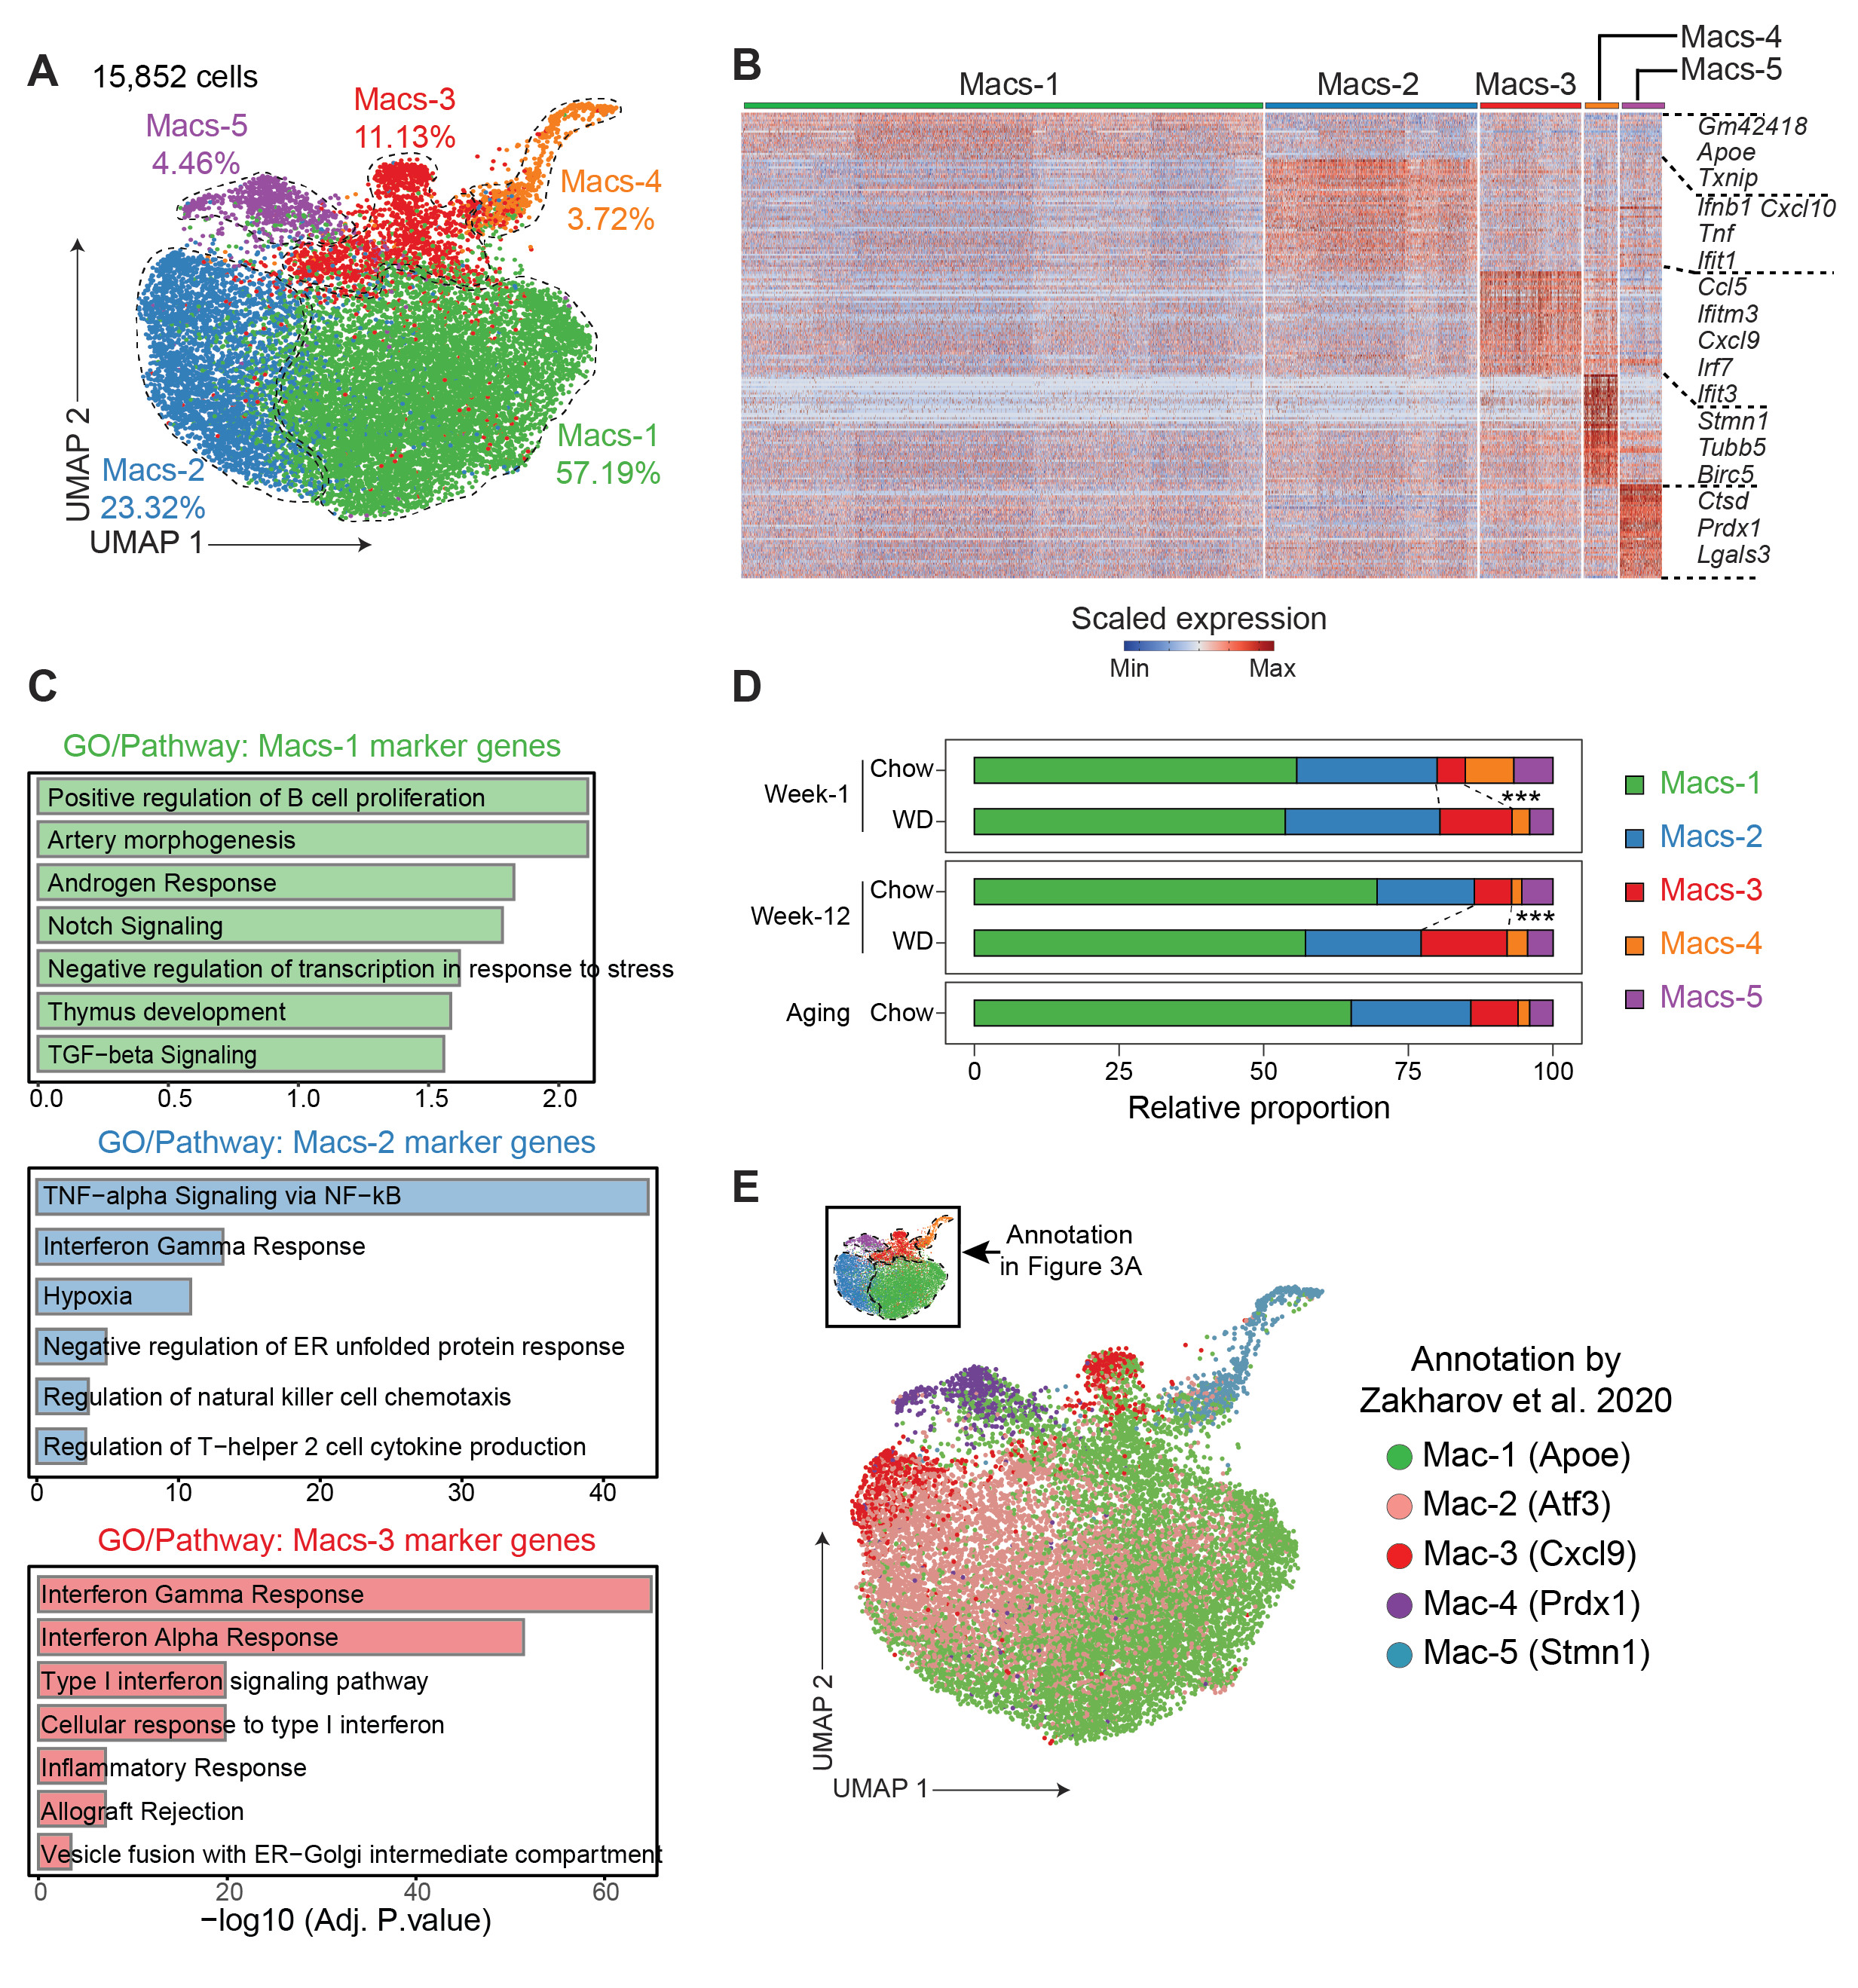
\includegraphics[width=\linewidth]{Chapter4/Fig/F2-5-01.png}
\caption[Characterization of islet-intrinsic macrophages using \glsentryshort{scr}]{\textbf{Characterization of islet-intrinsic macrophages using \gls{scr}}. \textbf{(A)} \gls{umap} embedding of pancreatic islet associated macrophages, pooled across three time-points (W1, W12 and Aging) and two dietary conditions (Chow and \gls{wd}). Values indicate the overall proportion of each defined sub-population. The identities of sub-populations were defined based on marker gene expression. \textbf{(B)} Heatmaps showing scaled expression levels of marker genes in each macrophage sub-population. \textbf{(C)} Enriched \gls{go} terms using top markers for the five macrophage sub-populations. Significance ($-\log_{10}$ adjusted p-value) of the enrichment are shown in bar plots. \textbf{(D)} The proportion of each macrophage sub-population in \textbf{(A)}, computed as a percentage of total macrophage cell numbers in every experimental group. The cells from different biological replicate cohorts were pooled together. $\textsuperscript{*} p < 0.05, \textsuperscript{**} p < 0.01, \textsuperscript{***} p < 0.001$. p-values were calculated from a mixed-effects binomial model. }
\label{fig:chp2_scrna_macrophages}
\end{figure}

% \begin{wrapfigure}{r}{0.5\textwidth}
% \vspace{-20pt} 
% 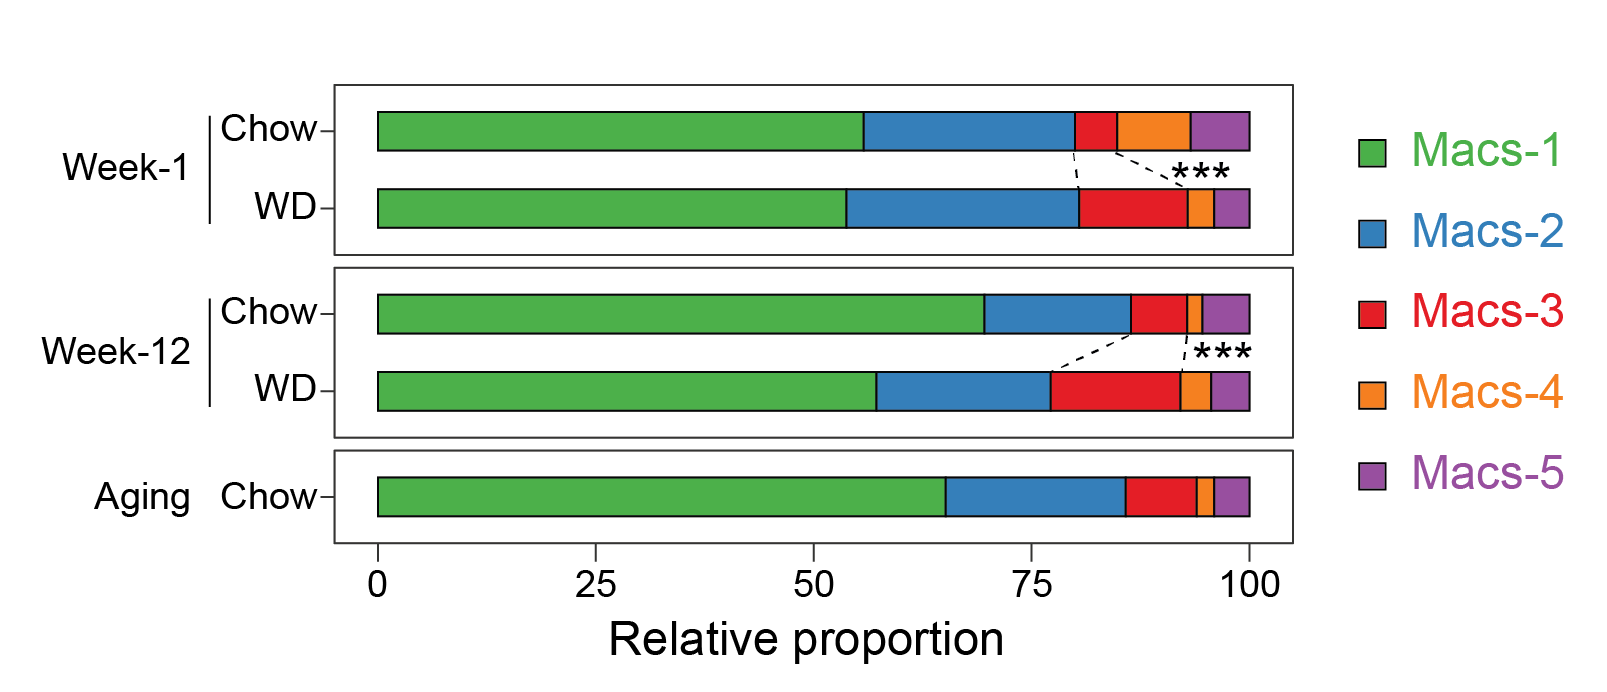
\includegraphics[width=7.5cm]{Chapter4/Fig/F2-5-03.png}
% \caption[Proportions of islet-intrinsic macrophages]{\textbf{Relative proportions of islet macrophages across \gls{wd}-feeding and aging}. Proportion of each macrophage sub-population in \textbf{(\autoref{fig:chp2_scrna_macrophages} A)}, computed as a percentage of total macrophage cell numbers in every experimental group. The cells from different biological replicate cohorts were pooled together. *: p<0.05, **: p<0.01, ***: p<0.001. p-values were calculated from a mixed-effects binomial model.}
% \label{fig:chp2_scrna_macrophages_composition}
% \vspace{-10pt}
% \end{wrapfigure} This increase could be likely to further support islet homeostasis as the mice age. 

\par The proportion of the non-inflammatory Macs-1 was the highest among all islet macrophage sub-populations, with over 50\% of the cells identified as Macs-1 in all conditions \textbf{(\autoref{fig:chp2_scrna_macrophages} D)}. Intriguingly, the W12-Chow and the Aging-Chow groups exhibited a notable higher proportion of the homeostatic Macs-1 macrophages compared to their W1-Chow counterparts \textbf{(\autoref{fig:chp2_scrna_macrophages} D)}. There was a rapid and significant expansion of the Macs-3 macrophages in response to \gls{wd} feeding, and a comparable, albeit less obvious increase during aging \textbf{(\autoref{fig:chp2_scrna_macrophages} D)}. This mirrors the stress-induced accumulation of F4/80\textsuperscript{\textit{low}} macrophages not just in the pancreas, but also in the islets and the peri-islet region \textbf{(\autoref{fig:chp2_imc_macrophages2} A}, middle\textbf{; \autoref{fig:chp2_imc_macrophages2} B}, middle\textbf{)}. In addition to these shifts, while there was a marked decrease in the proportion of the proliferating Macs-4 macrophages in response to short-term \gls{wd} feeding for 1 week, the pro-inflammatory Macs-2 and the phagocytotic Macs-5 macrophages were relatively stable during the course of \gls{wd}-feeding and aging \textbf{(\autoref{fig:chp2_scrna_macrophages} D)}.

%\clearpage

\subsubsection{\large Mapping islet-macrophages from \glsentryshort{nod} mouse model of \glsentryshort{t1d}}

% \begin{wrapfigure}{l}{0.5\textwidth}
% 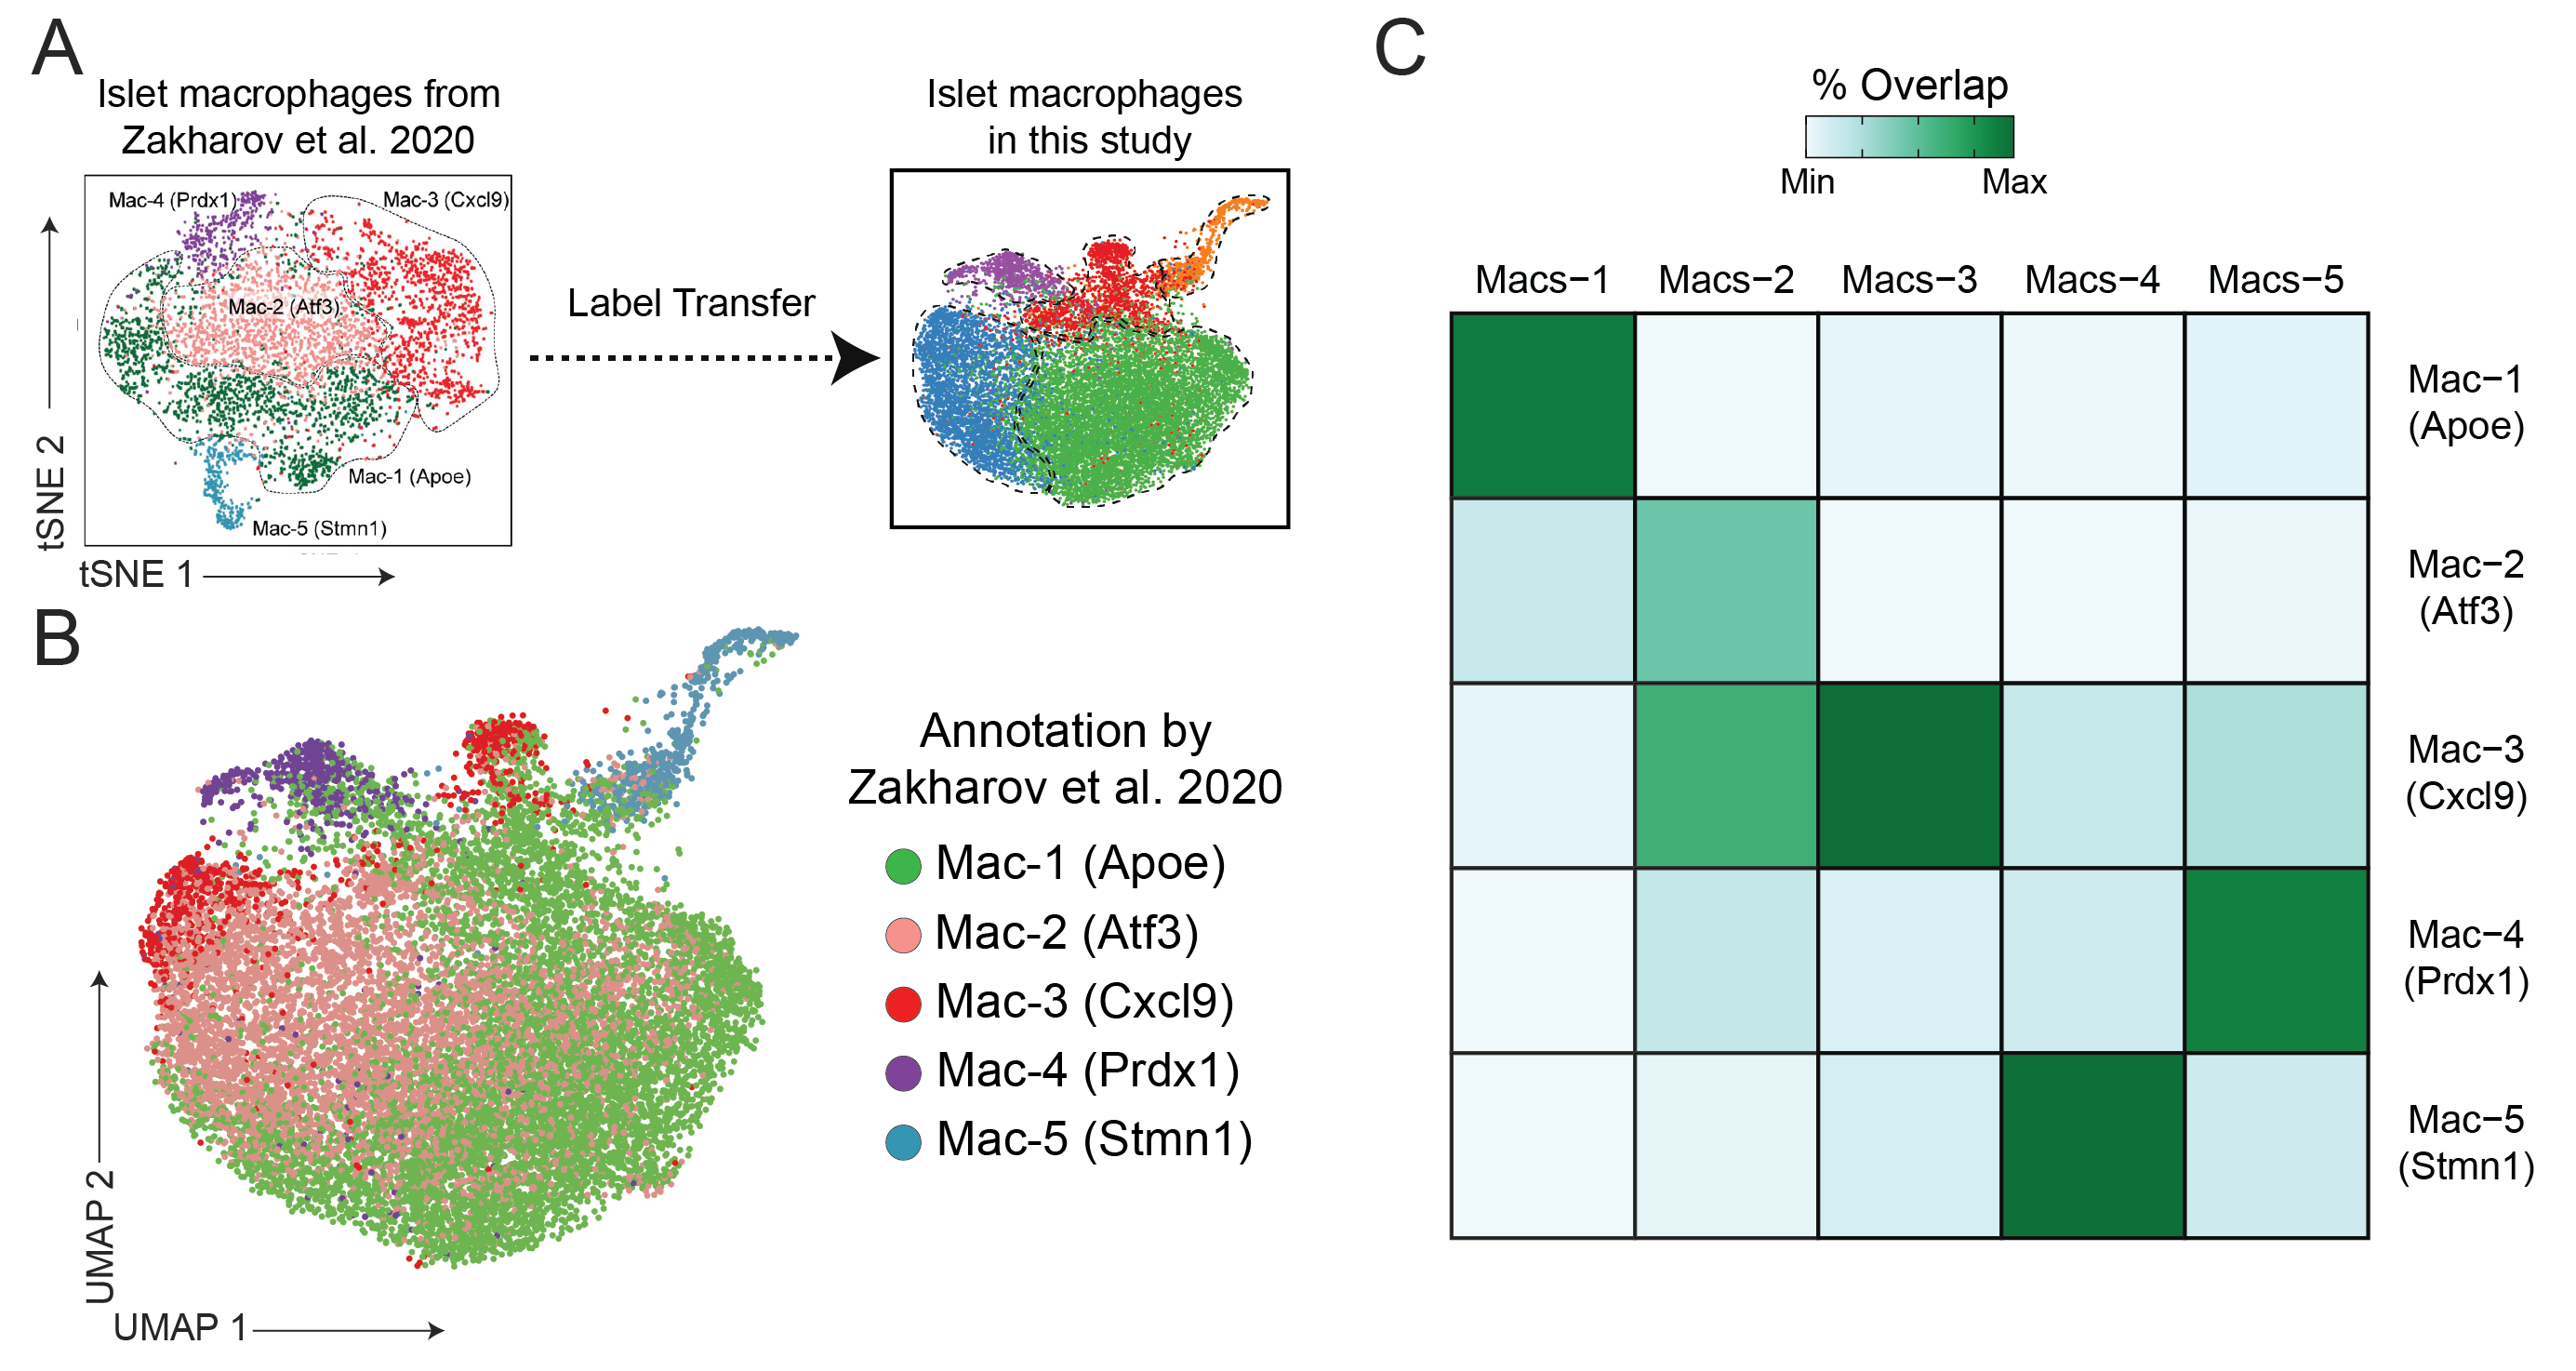
\includegraphics[width=8cm]{Chapter4/Fig/F2-5-02.png}
% \caption[res-macs3]{\textbf{Label transfer of annotations from Zakharov et. al}}
% \label{fig2-5-3}
% \end{wrapfigure}

A similar single-cell study of islet macrophages in a \gls{nod} mouse model identified five main macrophage sub-populations \textbf{\cite{zakharov_single-cell_2020}}. In the study by Zakharov \textit{et al.}, the authors identified a non-inflammatory sub-population, Mac-1 (\textit{Apoe}), characterized by elevated levels of \textit{Apoe} and \textit{Trem2}; two groups of inflammatory activated macrophages, Mac-2 (\textit{Atf3}), characterized by strong \gls{nfkb} activation and elevated expression of genes encoding inflammatory cytokines, and Mac-3 (\textit{Cxcl9}), which depicted elevated expression of genes encoding several cytokines, co-stimulatory molecules, and molecules involved in antigen presentation, alongside \gls{nfkb} signature. Apart from these three groups, the authors also identified Mac-4 (\textit{Prdx1}), associated with lysosomal activity and apoptotic cell clearance and Mac-5 (\textit{Stmn1}), associated with the cell-cycle pathway \textbf{(\autoref{fig:chp2_scrna_macrophages_unanue} A,} left\textbf{)}.\\

% \begin{wrapfigure}{l}{0.5\textwidth}
% \vspace{-20pt}
% 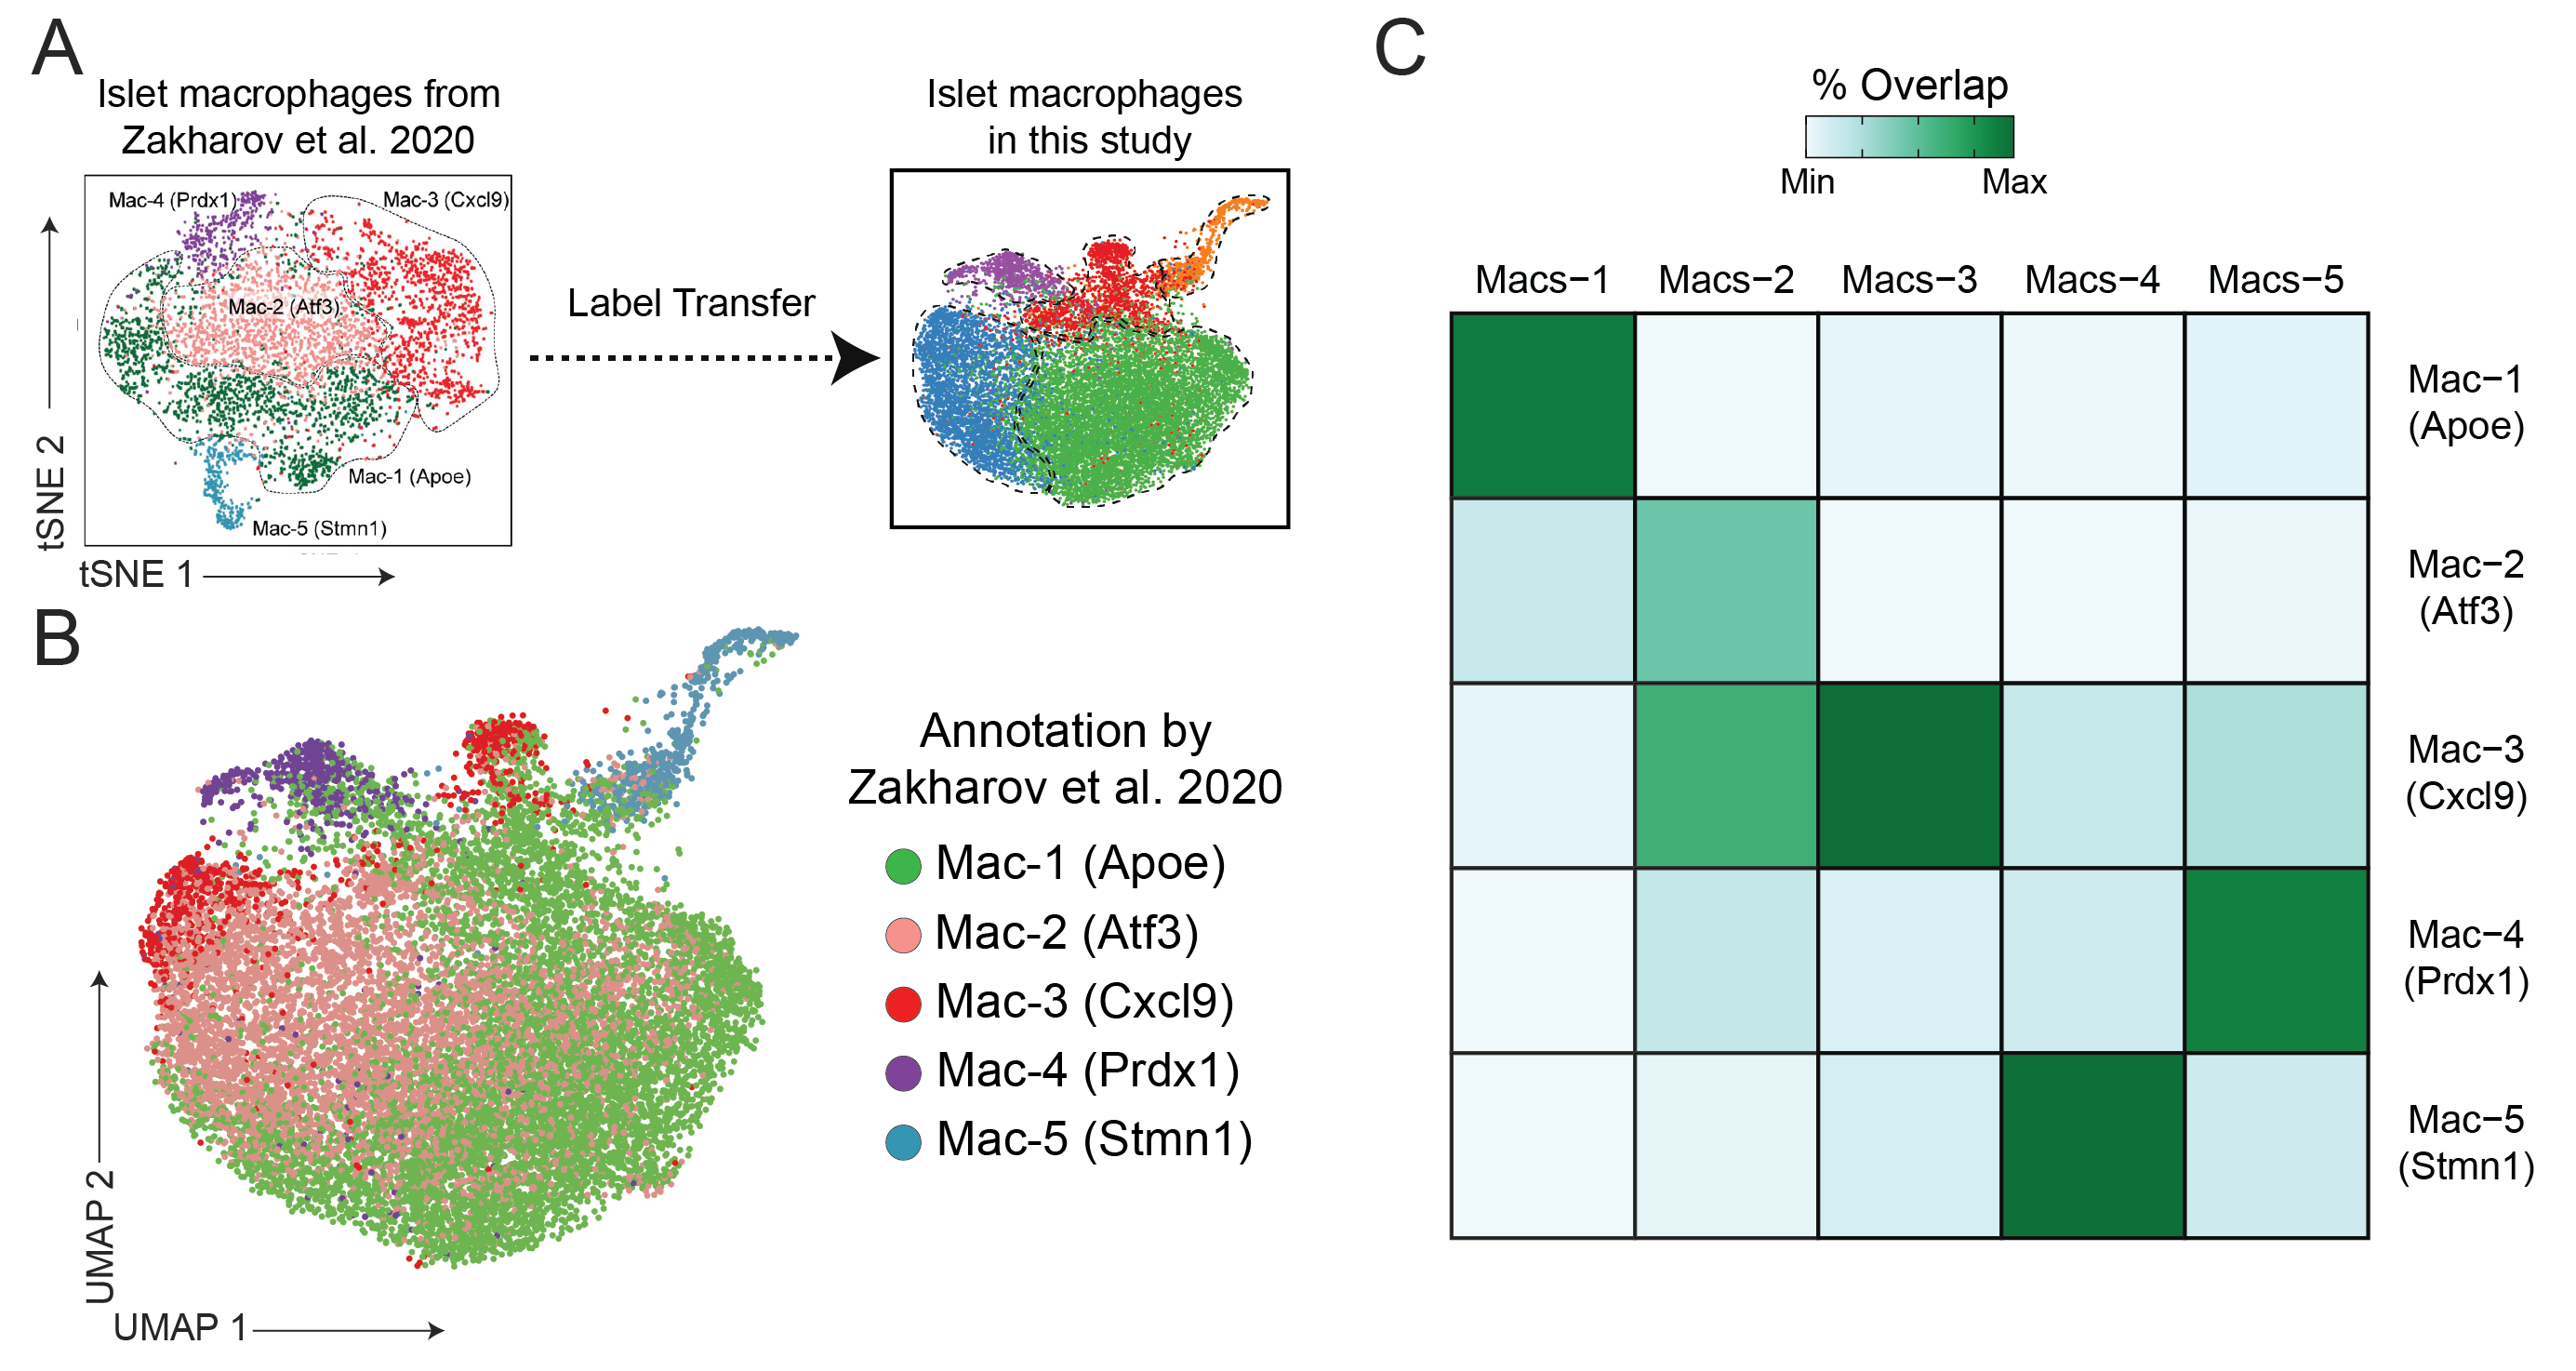
\includegraphics[width=7cm]{Chapter4/Fig/F2-5-02.png}
% \caption[Mapping islet macrophages from flp1{t1d}{T1D} \glslink{nod}{NOD} mice]{\textbf{Mapping islet macrophages from \glslink{t1d}{T1D} \glslink{nod}{NOD} mice.} \textbf{(A) Left:} \gls{tsne} embedding of islet macrophage populations characterized by Zakharov \textit{et al.}, illustrating the five distinct sub-populations. \textbf{(B)} \gls{umap} embedding of islet macrophages from this study, grouped according to annotations in panel \textbf{(A) Left} following the label transfer workflow.}
% \label{fig:chp2_scrna_macrophages_unanue}
% \vspace{-10pt}
% \end{wrapfigure}
\vspace{-20pt}
\begin{figure}[H]
\centering
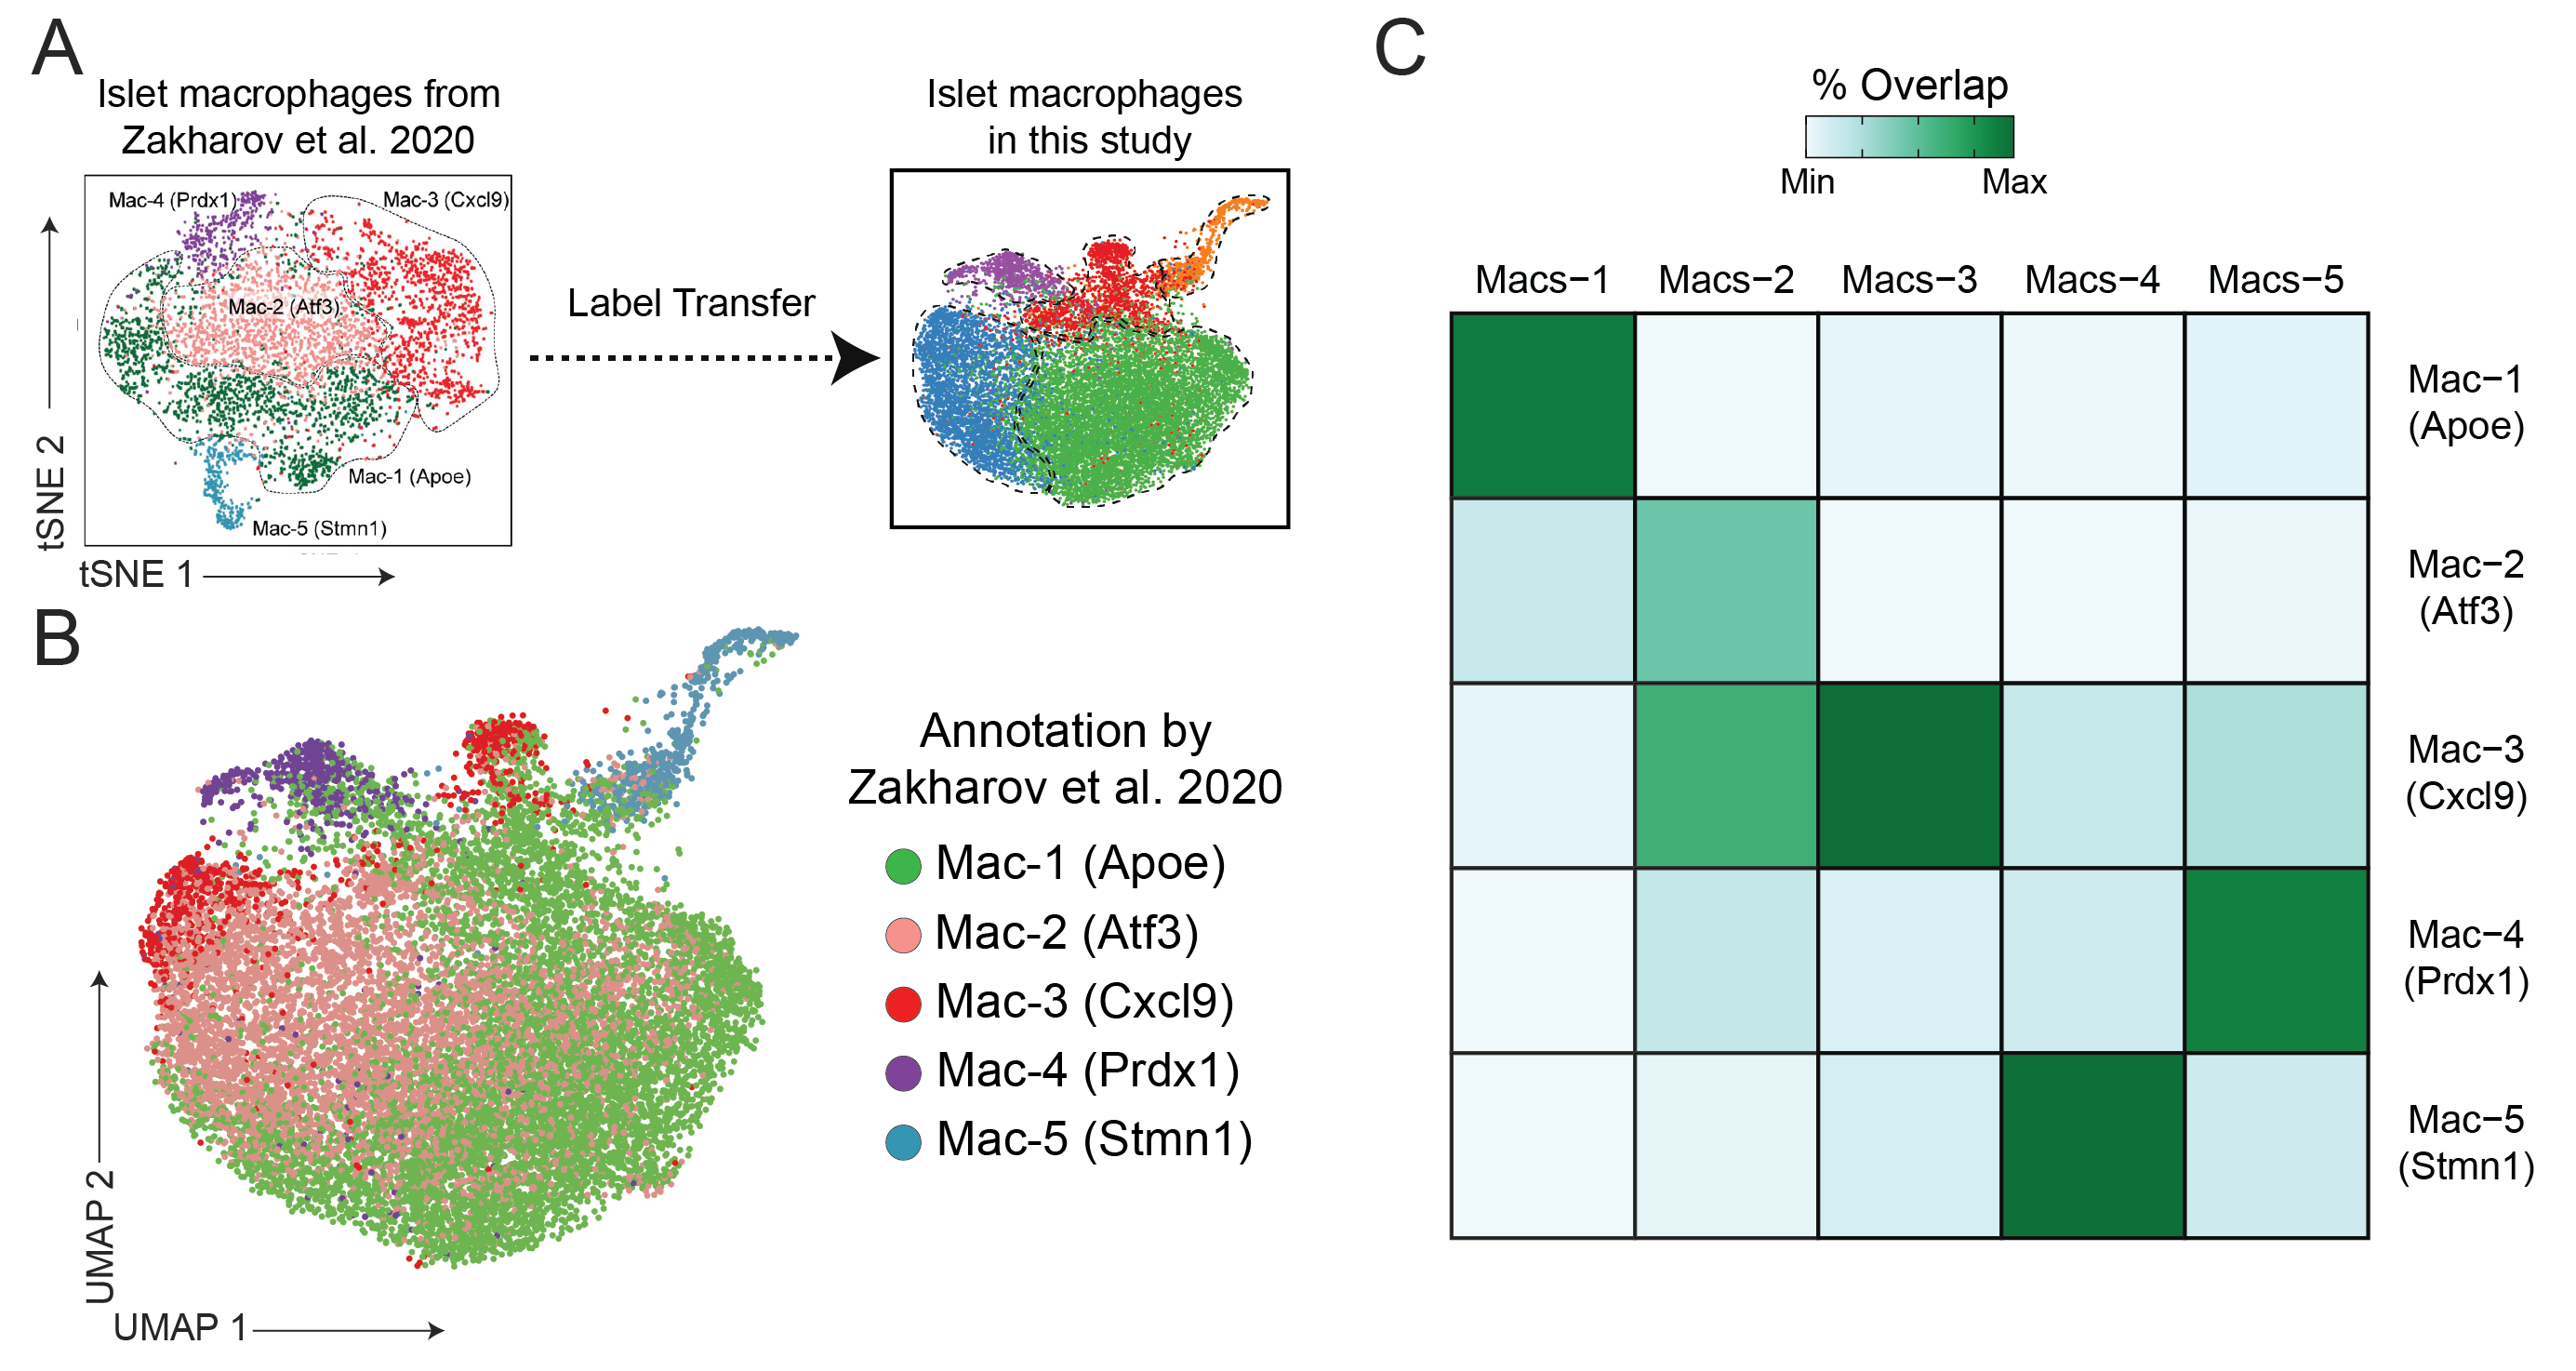
\includegraphics[width=13cm]{Chapter4/Fig/F2-5-02.png}
\caption[Mapping islet macrophages from \glsentryshort{nod} model of \glsentryshort{t1d}]{\textbf{Mapping islet macrophages from a \gls{nod} model of \gls{t1d}.} \textbf{(A)} Schematic depicting the label transfer workflow to map the annotations of the islet macrophages in the \gls{nod} model of \gls{t1d} onto the macrophages identified in this study. \textbf{(B)} \gls{umap} embedding of islet macrophages from this study, grouped according to annotations of the \gls{t1d} \gls{nod} mice islet macrophages, following the label transfer workflow. \textbf{(C)} Heatmap depicting the percentage of overlap of marker genes for the \gls{t1d} \gls{nod} mice islet macrophages (rows) and the islet macrophages from this study (columns).}
\label{fig:chp2_scrna_macrophages_unanue}
\end{figure}

\par Therefore, noting the transcriptomic similarities between the islet-intrinsic macrophages in the \gls{nod} model of \gls{t1d} and \gls{wd}-fed mice from our analysis, we performed label transfer and mapped these \gls{nod}-mice macrophage sub-populations onto our islet macrophages \textbf{(\autoref{fig:chp2_scrna_macrophages_unanue} A;} see \hyperref[subsubsec:met_chp2_labeltransfer]{\textbf{Methods}}\textbf{)}. This analysis revealed a strong correspondence in the islet-resident macrophage sub-populations between the two studies \textbf{(\autoref{fig:chp2_scrna_macrophages_unanue} B)}. In addition to this, there was also strong one-to-one overlap of marker genes for the macrophage sub-populations identified in the two studies \textbf{(\autoref{fig:chp2_scrna_macrophages_unanue} C)}. In the original study, Mac-1 and Mac-2 macrophages showed limited changes over time whereas Mac-3 was the only sub-population that showed continuous strong expansion during \gls{t1d} progression \textbf{\cite{zakharov_single-cell_2020}}. This echoes similar observation of limited composition shifts of Macs-1 and Macs-2 macrophages and the expansion of Macs-3 in response to \gls{wd} feeding in our analysis \textbf{(\autoref{fig:chp2_scrna_macrophages} D)}. Additionally, the Mac-3 sub-population was comprised of two distinct groups: a monocyte-derived Mac-3 macrophages which expressed a number of monocyte markers (\textit{Ccr2,Plac8} and \textit{Ly6c1}); and a resident-macrophage developed Mac-3 group which lacked monocytic markers. This heterogeneity within Mac-3 was also apparent upon label transfer as the Mac-3 sub-population mapped partially to Macs-2 and Macs-3 and also in the overlap of the marker genes of the two corresponding sub-populations \textbf{(\autoref{fig:chp2_scrna_macrophages_unanue} B,C)}, with cells in Macs-2 expressing the monocytic marker \textit{Ccr2} \textbf{(\autoref{fig:app_scrna_macrophages_macs2_genes} B)}. Contrary to the decreased proportion of anti-inflammatory Mac-4 during autoimmunity progression, the proportion of the corresponding Macs-5 sub-population was unchanged in response to \gls{wd} feeding or aging \textbf{(\autoref{fig:chp2_scrna_macrophages} D)}.\\

\par In conclusion, the annotation mapping highlighted significant transcriptomic parallels between the islet-intrinsic macrophages in \gls{nod} model of \gls{t1d} and those in \gls{wd}-fed and old mice. 


% to show continuous strong expansion during \gls{t1d} progression



% <ADD MORE SENTENCES>

%\clearpage


\subsubsection{\large Linking macrophage sub-populations from \gls{scr} to \gls{imc}}

To establish a link between the macrophage sub-populations identified in our single-cell analysis and those determined through the \gls{imc} analysis, we examined, in our \gls{scr} dataset, the expression of marker genes corresponding to the \gls{imc} channels used for the classification of macrophages. Our investigation indicated that F4/80 expression was highest in Macs-1, lower in Macs-3, and lowest in Macs-2 \textbf{(\autoref{fig:chp2_scrna_macrophages_imc} A,} top\textbf{)}. Observing a similar pattern in the \gls{imc} analysis, we linked Macs-1, Macs-2, and Macs-3 macrophage sub-populations in the \gls{scr} dataset to the F4/80\textsuperscript{\textit{high}}, F4/80\textsuperscript{-}, and F4/80\textsuperscript{\textit{low}} sub-populations, respectively. Specifically, Macs-3, akin to the F4/80\textsuperscript{\textit{low}} sub-population, showed moderate F4/80 channel (\textit{Adgre1}) expression but exhibited the highest levels of CD11c (\textit{Itgax}) and CD69 (\textit{Cd69}) channel expression as signs of activation \textbf{(\autoref{fig:chp2_scrna_macrophages_imc} B)}. Moreover, the proliferative Macs-4 macrophages likely equates to the KI67\textsuperscript{\textit{high}} macrophages observed in the \gls{imc} analysis \textbf{(\autoref{fig:chp2_scrna_macrophages_imc} A} top\textbf{, B)}. We did not find an equivalent for the Macs-5 sub-population in the preceding \gls{imc} analysis, suggesting possible discrepancies between protein-based and \glsentryshort{rna}-based methodologies for cell type annotation. To further confirm the resemblance between the Macs-3 and F4/80\textsuperscript{\textit{low}} sub-populations, we examined the expression of these marker genes under \gls{wd} feeding and aging conditions. The Macs-3 sub-population manifested an augmented inflammatory phenotype under both conditions, as evidenced by the up-regulated gene expression of CD11c (\textit{Itgax}) and CD69 (\textit{Cd69}) \textbf{(\autoref{fig:chp2_scrna_macrophages_imc} A,} bottom\textbf{)}. This inflammatory modulation parallels observations in the F4/80\textsuperscript{\textit{low}} cells as elucidated from the \gls{imc} analysis \textbf{(\autoref{fig:chp2_scrna_macrophages_imc} C)}.\\


\begin{figure}[t!]
\centering
%\vspace{-25pt}
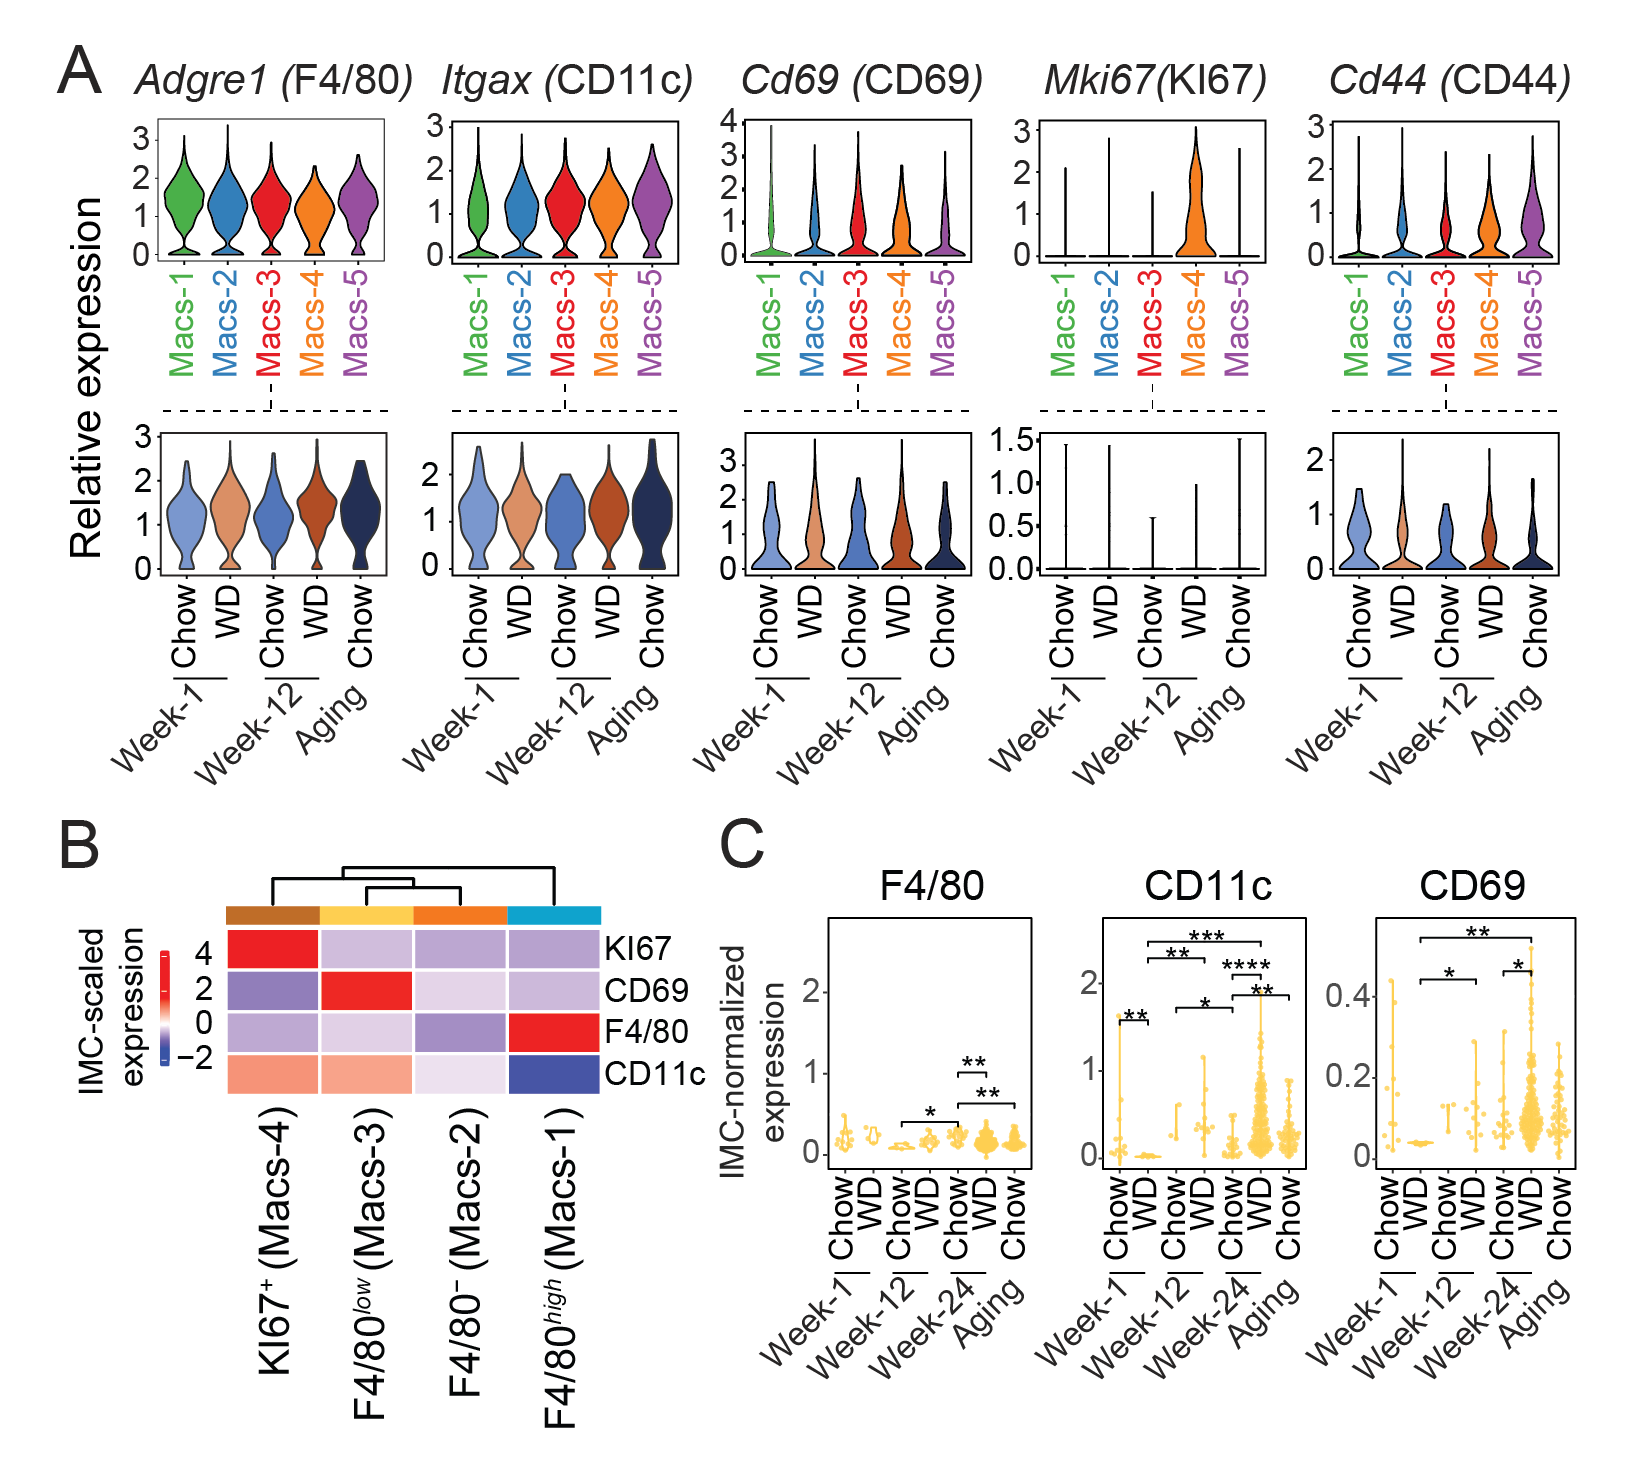
\includegraphics[width=\linewidth]{Chapter4/Fig/F2-4-01.png}
\caption[Linking macrophage sub-populations from \glsentryshort{scr} to \glsentryshort{imc}]{\textbf{Linking macrophage sub-populations from \gls{scr} to \gls{imc}.} \textbf{(A)} Violin plots depicting the normalized expression levels of genes with corresponding channels in the \gls{imc} panel. The top row depicts the expression across various macrophage sub-populations, and the bottom row depicts their expression in the Macs-3 sub-population under across the experimental groups. \textbf{(B)} Heatmap showing \textit{z-score} expression of selected \gls{imc} channels across the four macrophage sub-populations identified in the \gls{imc} analysis. Corresponding macrophage sub-populations from \gls{scr} data are indicated in parantheses. \textbf{(C)} Violin plots of \textit{arcsinh} transformed expression of selected channels in the F4/80\textsuperscript{\textit{low}} macrophage sub-population from the \gls{imc} analysis across the experimental groups. *p<0.05, **p<0.01, ***p<0.001 and ****p<0.0001. p-values were calculated using the Wilcoxon rank-sum test with Bonferroni correction. \textit{The data and figure in } \textbf{(B)} \textit{and} \textbf{(C)} \textit{were originally generated by Dr. Matthias Barone and reused here with permission.}}
\label{fig:chp2_scrna_macrophages_imc}
\end{figure}




\par Collectively, we identified macrophage sub-populations with distinct activation status in the pancreatic islets. Our findings underscore age-related accumulation and activation of inflammatory Macs-3 (F4/80\textsuperscript{\textit{low}}) macrophages within pancreatic islets, a phenomenon that is markedly amplified under over-nutrition conditions.

%\clearpage

% \mysidecaption{0.4}{%
% \captionof{figure}{\textbf{Linking macrophage sub-populations between scRNA-seq and IMC analyses.} \textbf{(A)} Violin plots depicting the normalized expression levels of selected markers with corresponding channels in the IMC panel. The top plots compare these levels across various macrophage sub-populations, and the bottom plots display their expression in the Macs-3 population under different experimental conditions. \textbf{(B)}Heatmap showing z-scored expression of selected IMC channgels across the four macrophage sub-populations identified in the IMC analysis. Corresponding macrophage sub-populations from scRNA-seq analysis are indicated in parantheses. \textbf{(C)} Violin plots of \textit{arcsinh} transformed expression of selected IMC channels in the F4/80\textsuperscript{\textit{low}} macrophage sub-population from the IMC analysis across experimental conditions. * p<0.05, ** p<0.01, *** p<0.001 and **** p<0.0001. p-values were calculated using the Wilcoxon rank-sum test with Bonferroni correction.}%
% }
% {%
% 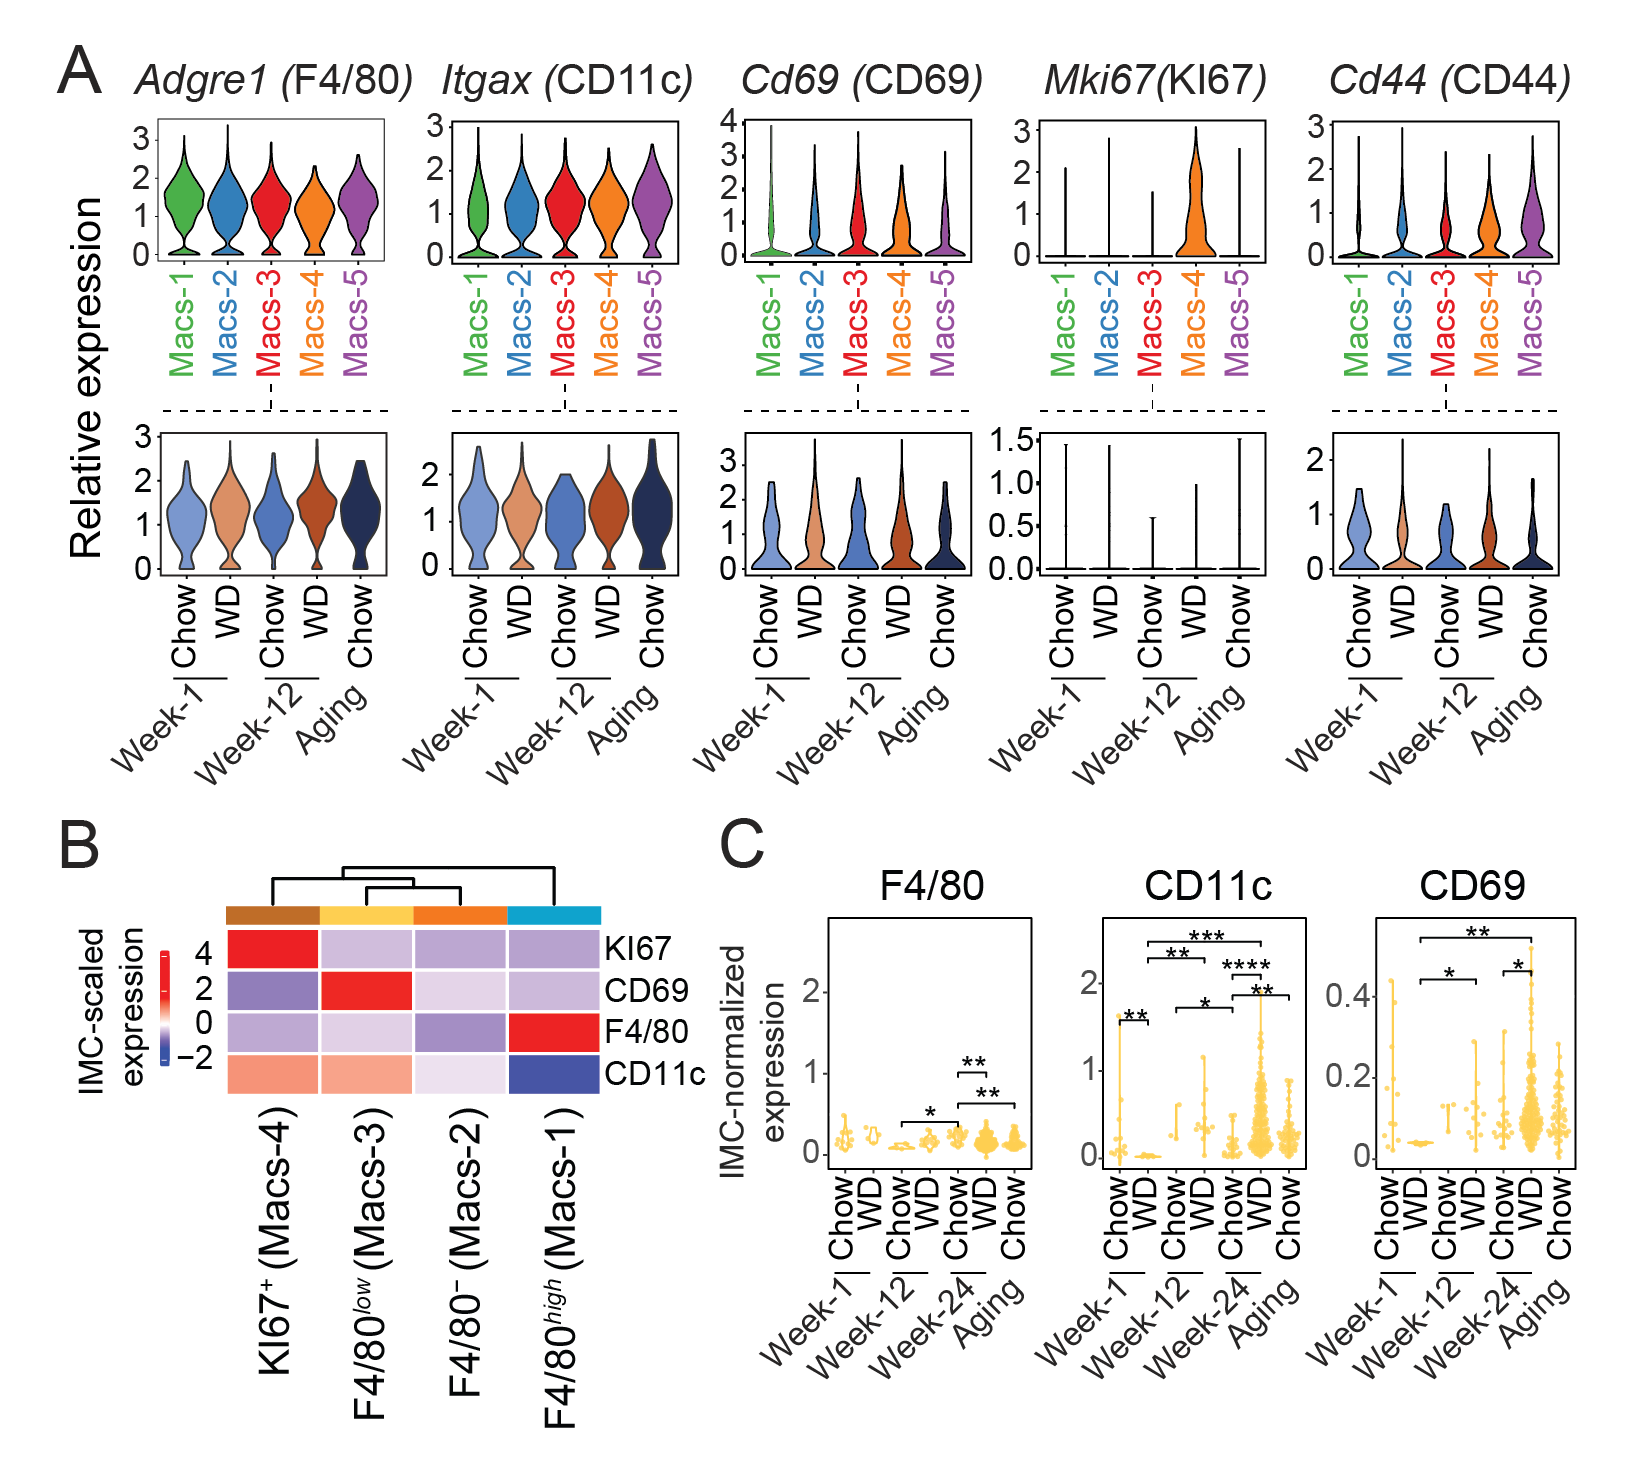
\includegraphics[width=9cm,height=11cm,keepaspectratio]{Chapter4/Fig/F2-4-01.png}%
% }[t]%

% \begin{wrapfigure}{r}{0.5\textwidth}
% 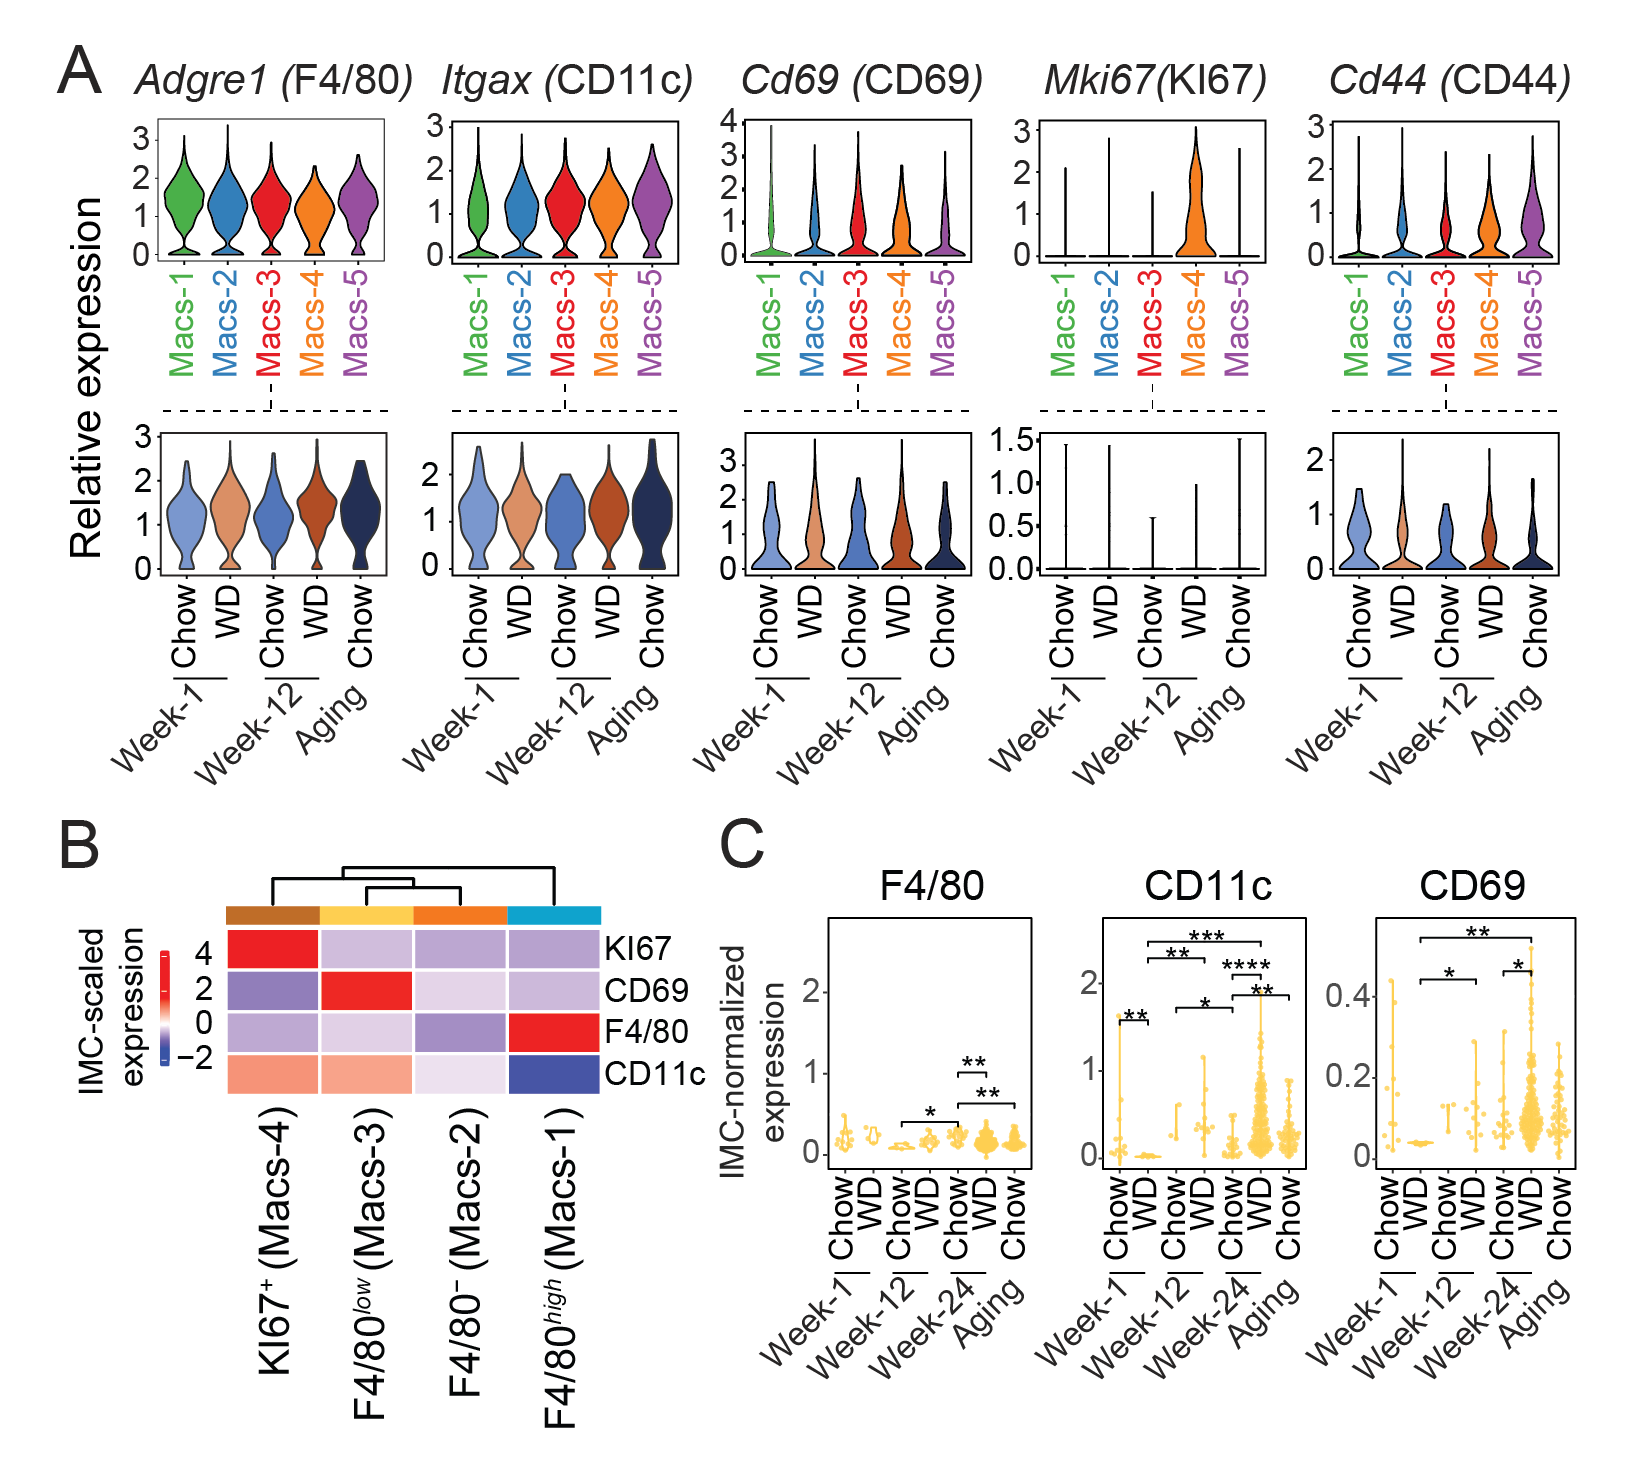
\includegraphics[width=9cm,height=11cm,keepaspectratio]{Chapter4/Fig/F2-4-01.png}
% \caption[]{\textbf{Linking macrophage sub-populations between scRNA-seq and IMC analyses.}}
% \label{fig2-4}
% \end{wrapfigure}

% \begin{SCfigure}[][h]
% \centering
% 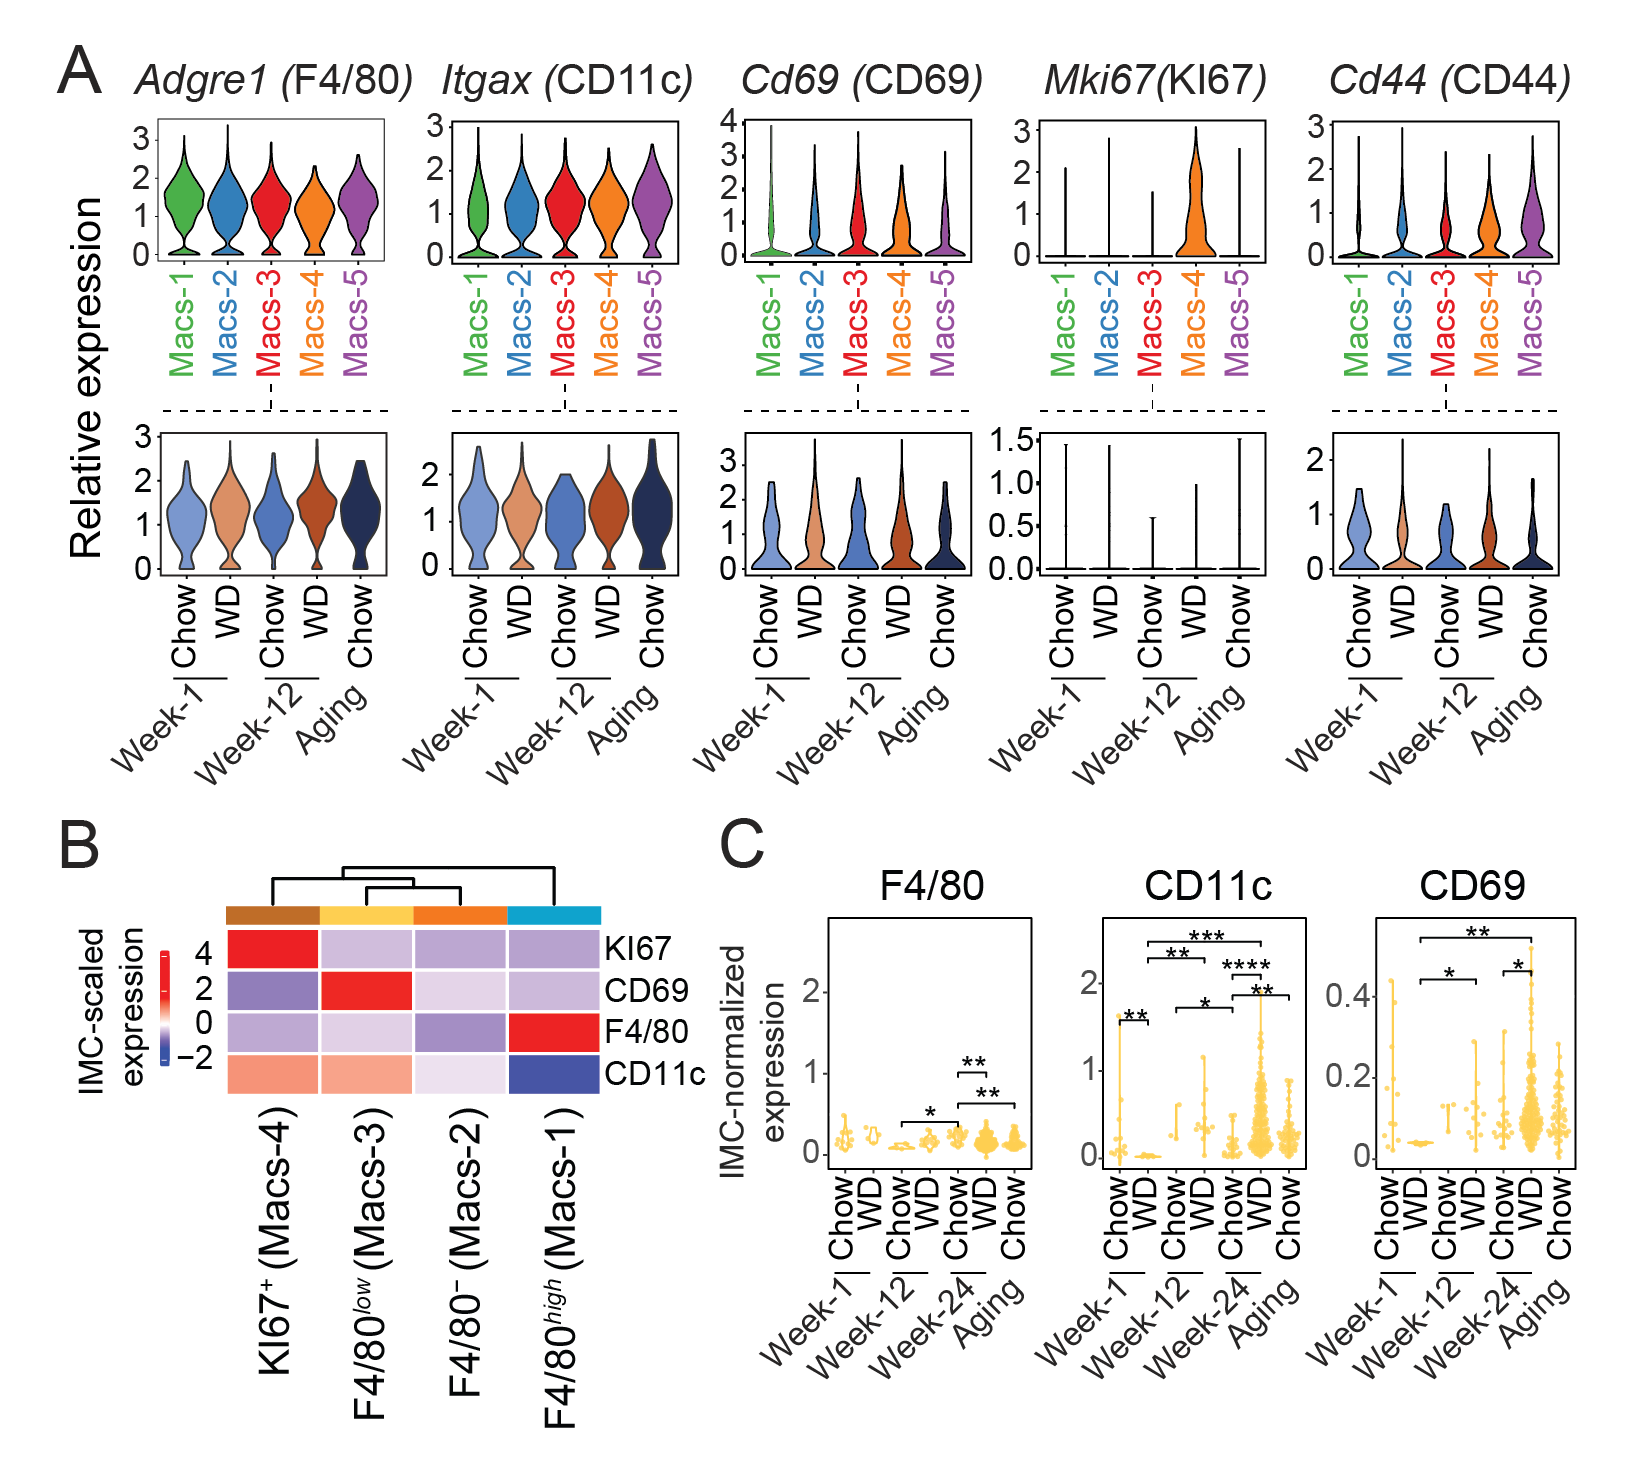
\includegraphics[width=8cm]{Chapter4/Fig/F2-4-01.png}
% \caption[res-macs2]{\textbf{Linking macrophage sub-populations from scRNA-seq to IMC}\\
% \textbf{(A)} Violin plots depicting the normalized expression levels of genes with corresponding channels in the IMC panel. The top plots compare these levels across various macrophage sub-populations, and the bottom plots display their expression in the Macs-3 population under different experimental conditions. \textbf{(B)}Heatmap showing z-scored expression of selected IMC channgels across the four macrophage sub-populations identified in the IMC analysis. Corresponding macrophage sub-populations from scRNA-seq analysis are indicated in parantheses. \textbf{(C)} Violin plots of \textit{arcsinh} transformed expression of selected IMC channels in the F4/80\textsuperscript{\textit{low}} macrophage sub-population from the IMC analysis across experimental conditions. *p<0.05, **p<0.01, ***p<0.001 and ****p<0.0001. p-values were calculated using the Wilcoxon rank-sum test with Bonferroni correction.} 
%  \label{fig2-4}
% \end{SCfigure}

% \begin{SCfigure}[1][h]
% \centering
% \caption[res-macs2]{\textbf{Linking macrophage sub-populations from scRNA-seq to IMC}. \textbf{(A)} Violin plots depicting the normalized expression levels of selected markers with corresponding channels in the IMC panel. The top plots compare these levels across various macrophage sub-populations, and the bottom plots display their expression in the Macs-3 population under different experimental conditions. \textbf{(B)}Heatmap showing z-scored expression of selected IMC channgels across the four macrophage sub-populations identified in the IMC analysis. Corresponding macrophage sub-populations from scRNA-seq analysis are indicated in parantheses. \textbf{(C)} Violin plots of \textit{arcsinh} transformed expression of selected IMC channels in the F4/80\textsuperscript{\textit{low}} macrophage sub-population from the IMC analysis across experimental conditions. * p<0.05, ** p<0.01, *** p<0.001 and **** p<0.0001. p-values were calculated using the Wilcoxon rank-sum test with Bonferroni correction.
% }
% 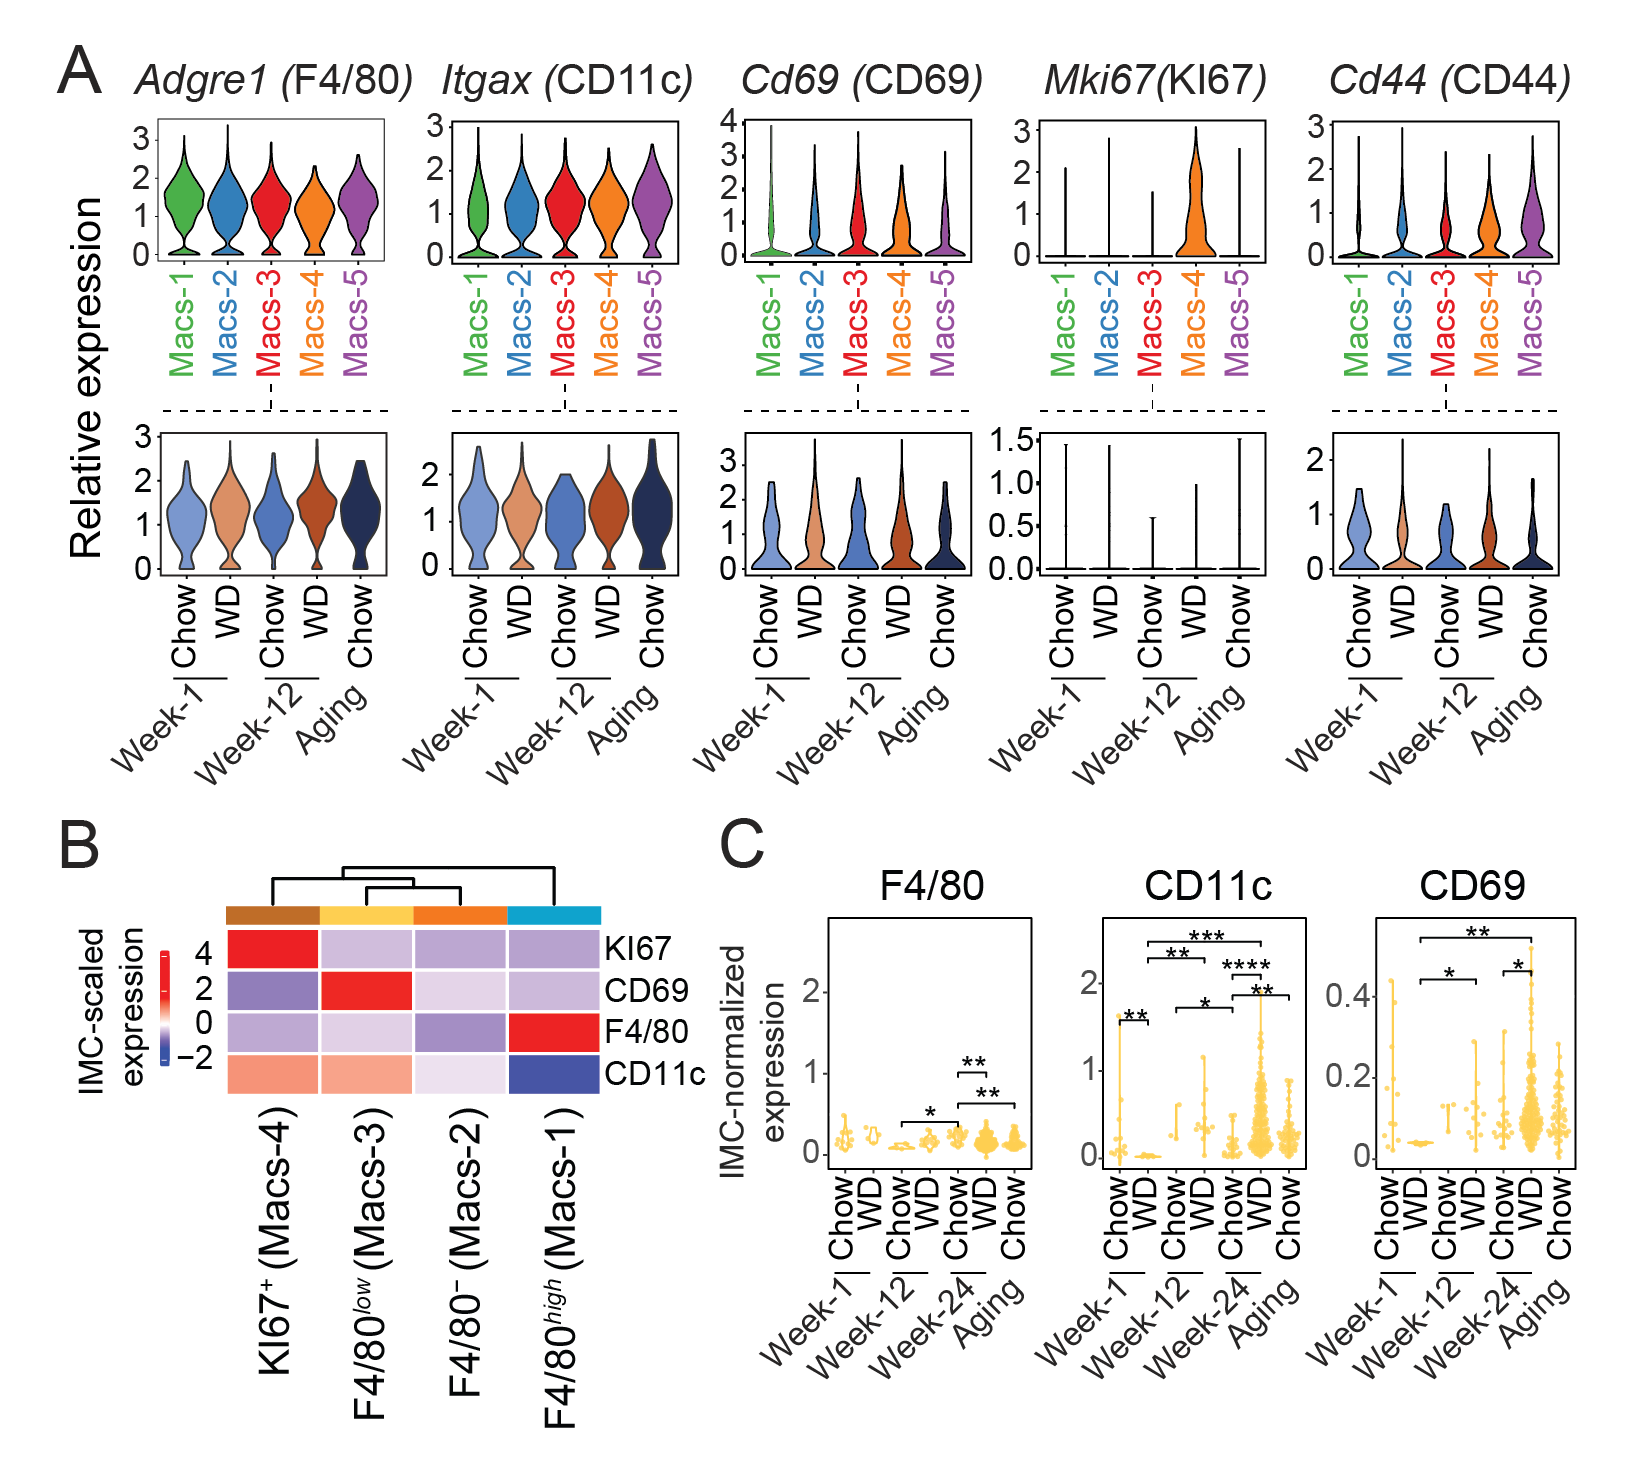
\includegraphics[width=0.6\textwidth]{Chapter4/Fig/F2-4-01.png}
% \label{fig2-4}
% \end{SCfigure}
% \subsubsection{Demultiplexing donors from pooled experiments} 
% \st{Interestingly, despite Macs-2 exhibiting a lower activation profile compared to Macs-3, WD feeding resulted in a stronger expression of genes coding for inflammatory cytokines and chemokines in Macs-2 (Figure S4D,E). In contrast, this induced upregulation of cytokine genes observed in Macs-2 under WD feeding conditions is not evident in the aging condition (Figure S4F)}


% In the considered pooled experimental design, cells from multiple donors are differentiated together in the same experiment. 
% To be able to link the genetic background of an individual with their transcriptional profile we need to map the cells back to their donor of origin, without the use of any barcode.
% Indeed, we find that for the large majority of cells the RNA-seq reads map to a sufficient number of common genetic variants for us to reliably assign each cell to its original donor.
% In particular, assignment of cells to donors was performed using Cardelino \cite{mccarthy2020cardelino}. 
% In short, Cardelino estimates the posterior probability of a cell originating from a specific donor using common genetic variants in \gls{scrnaseq} reads, while employing a Bayesian beta binomial-based approach to account for technical factors such as differences in read depth, allelic drop-out, and sequencing accuracy. 
% To perform donor assignment, we considered a larger set of \gls{hipsci} lines with genotype information (n=490), including the 126 lines used in this study. 
% A cell's assignment to a donor was considered successful if the model identified the match i) with posterior probability > 0.9, and ii) using a minimum of 10 informative variants. 
% Cells for which the donor identification was not successful were discarded and not considered for further analyses.
% Across the entire dataset, 99\% of cells that passed RNA QC steps (see below) were successfully assigned to a donor.
% In some cases, unexpected donor assignment (where several cells from one experiment were found to be assigned to none of the 4-6 donors used in that experiment) allowed me to identify (and correct) plate swaps that happened in the lab, without losing any data (\textbf{Fig. \ref{fig:plate_swap}}).

% \begin{figure}[h]
% \centering
% \includegraphics[width=14cm]{Chapter4/Fig/cardelino_example.png}
% \caption[Demultiplexing donors]{\textbf{Demultiplexing donors}.\\
% Example of how donor assignment of cells helped identifying a plate swap.
% To explore the results of the donor assignment algorithm \cite{mccarthy2020cardelino}, I plotted cells along two axes: on the x axis, the posterior probability of being assigned to a certain donor, on the y the number of common variants found on \gls{scrnaseq} reads used to perform the assignment.
% Because we know for each experiment which lines are supposed to have been differentiated, we can colour cells based on whether the donor they have been assigned to was used in the specific experiment or not.
% On the left, an example of a correct donor assignment: most cells are assigned to one of the correct donors\footnotemark and the few that are not had very few usable genetic variants.
% On the right, the donor assignment is apparently incorrect.
% Most cells were assigned to donors that were not differentiated in the experiment, in many cases with a high level of confidence and using many variants, which would generally indicate high quality cells.
% Indeed, investigating further we realised that all cells were assigned to donors that all belonged to the same experiment, but that it was a different experiment.
% The wrong label was assigned in the lab: run 225216 actually contained cells from experiment 43 and not 39.
% By resolving this computationally, we avoided mistakes and retained all of the cells from this sequencing run, which would have otherwise been discarded.}
% \label{fig:plate_swap}
% \end{figure}


%\subsubsection{Flow cytometry}

% The success of the differentiation protocol was validated using expression of two protein surface markers, a pluripotency marker, Tra-1-60, and a marker of definitive endoderm, CXCR4. 
% We note that while cells were gated using the two markers, we did not discard any cells based on their expression. 
% In contrast, the first cell QC step performed using \gls{facs} consisted in identifying dead cells based on 7AAD\footnote{Staining with 7AAD is used a cell viability assay.
% 7AAD cannot readily pass through intact cell membranes, thus only cells with compromised membranes will stain.} using \gls{facs} staining.
% These were discarded and were not plated. 
% \gls{facs} data were analysed using the openCyto package, implemented in R \cite{finak2014opencyto}.
% The \gls{facs} gating strategy we used is illustrated in \textbf{Fig. \ref{fig:endodiff_facs_strategy}}.

% \begin{figure}[h]
% \centering
% \includegraphics[width=14cm]{Chapter4/Fig/endodiff_facs_strategy.png}
% \caption[FACS gating strategy]{\textbf{FACS gating strategy}.\\
% Figure by Mariya Chhatriwala.
% \gls{facs} gating strategy: first, single cells were stained with 7AAD to exclude dead cells. 
% Unstained live cells were then used to gate for expression of Tra-1-60 and CXCR4.}
% \label{fig:endodiff_facs_strategy}
% \end{figure}


% \newpage

% % footnote from plate swap figure (to make it appear on right page)
% \footnotetext{A cell technically could still have been assigned to a wrong donor within the correct experiment, but given a threshold both on the variants used (> 10) and on the posterior probability (> 0.9) I deemed this unlikely.}

%\subsubsection{scRNA-seq feature quantification and quality control}

% Single cell profiles were obtained using the SmartSeq2 technology \cite{picelli2013smart}. 
% This is a plate-based technology that involves single cells being sorted into 384 independent wells on a plate. 
% Adaptors of raw \gls{scrnaseq} reads were trimmed using Trim Galore! \cite{galore2015wrapper, martin2011cutadapt, andrews2010fastqc}, using default settings. 
% Trimmed reads were mapped to the human genome (build 37) using STAR \cite{dobin2013star}. 
% Gene-level expression quantification was performed using Salmon \cite{patro2017salmon}. 
% Briefly, Salmon quantifies transcript- (rather than gene-) level expression levels, similar to Kallisto \cite{bray2016near}.
% Then, such values are summarised at a gene level (\gls{cpm}).\\

% We performed \gls{qc} of \gls{scrnaseq} profiles following a widely used pipeline (see \textbf{section \ref{sec:scrnaseq}}) using Bioconductor packages \textit{scater} and \textit{scran}, implemented in R \cite{lun2016step, mccarthy2017scater, lun2019singlecellexperiment}.  
% In particular, cells were retained for downstream analysis if they had at least 50,000 counts from endogenous genes, at least 5,000 genes with non-zero expression, if less than 90\% of counts came from the top 100 most highly-expressed genes, less than 15\% of reads mapped to mitochondrial (MT) genes, they had a Salmon mapping rate of at least 60\%, based on distribution observation and thresholding (\textbf{Fig. \ref{fig:endodiff_qc_distributions}}) \cite{luecken2019current}.
% Additionally, cells were only retained if they could be successfully assigned to a donor (QC1, \textbf{Fig. \ref{fig:endodiff_qc_workflow}}). \\ 

% I then performed an additional QC step, where I excluded all cells from plates and experiments that had overall low quality.
% In the case of plates sequenced twice, I retained the one with most cells.
% Finally, I retained plates that had enough cells for the majority of the donors considered (QC2, \textbf{Fig. \ref{fig:endodiff_qc_workflow}}). 

% \begin{figure}[h]
% \centering
% \includegraphics[width=16cm]{Chapter4/Fig/endodiff_qc_examples.png}
% \caption[Distributions of QC metrics]{\textbf{Distributions of QC metrics}.\\
% Distributions of three exemplar QC metrics for six differentiation experiments (40-45).
% Shown are the cell distributions along the metrics (number of genes detected, percentage of counts from mitochondrial genes, Salmon \cite{patro2017salmon} mapping rate), as well as the thresholds we used as dotted lines, stratified by day and experiment.
% One can immediately spot how poor quality plates\footnotemark  perform similarly badly across all metrics (i.e. < 5,000 genes detected, <60\% reads mapped by Salmon).}
% \label{fig:endodiff_qc_distributions}
% \end{figure}

% \begin{figure}[h]
% \centering
% \includegraphics[width=16cm]{Chapter4/Fig/endodiff_qc_workflow.png}
% \caption[QC workflow]{\textbf{QC workflow}.\\
% Two stages of cell QC.
% First, at the level of single cells, all QC metrics and thresholds are indicated.
% 61\% of cells passed QC1.
% Second, at the experiment/plate level.
% If plates had many cells not passing QC1 they were considered poor quality batches and removed altogether.
% This stage removed far fewer cells, with 96\% of cells considered passing QC2.}
% \label{fig:endodiff_qc_workflow}
% \end{figure}


%\subsubsection{scRNA-seq processing}

% SmartSeq2 data do not include \glspl{umi}, which can be used to accurately detect PCR duplicates and quantify transcript abundance \cite{smith2017umi, islam2014quantitative, kivioja2012counting}. 
% In the absence of \glspl{umi}, we can borrow information from cells with similar total number of reads and correct for overall library size. 
% Such size factor normalisation of counts was performed using \textit{scater} \cite{mccarthy2017scater}. 
% %  \\
%  % footnote from qc examples figure (to make it appear on right page)
% \footnotetext{e.g. cells from day0, experiment 42.}
% Expressed genes with an HGNC symbol were retained for analysis, where expressed genes in each batch of samples were defined based on (i) raw count >100 in at least one cell prior to cell QC (i.e. \textbf{Fig. \ref{fig:endodiff_qc_workflow}}) and (ii) average log2(CPM+1) >1 after cell QC. 
% Normalised CPM data were log transformed (log2(CPM+1)) for all downstream analyses. 
% As a last QC step, we considered possible differences between cell lines derived from healthy and diseased donors. 
% Specifically, a subset of 11 cell lines in our dataset were derived from monogenic neonatal diabetes patients, and differentiated together with cell lines from healthy donors across 7 differentiation experiments (out of 28). 
% There was no significant difference in differentiation efficiency (see \textbf{section \ref{sec:endodiff_differentiation_efficiency}}) between healthy and neonatal diabetes lines in these experiments (p value > 0.05), and cells from both sets of donors overlapped in principal component space (\textbf{Fig. \ref{suppl_fig:pca_diabetes_lines}}). 
% Thus, we included cells from all donors in our analyses, irrespective of disease state.
%\newpage

\section[Aging and metabolic stress activate distinct type-1 \glsentryshort{ifn} responses in accumulating inflammatory macrophages]{Aging and metabolic stress activate distinct type-1 \gls{ifn}\\responses in accumulating inflammatory macrophages}
\label{sec:chp2_sc_macs3_diff}

\par The observed enrichment of the type-1 \gls{ifn}-responsive macrophage sub-population, Macs-3, during both \gls{wd} feeding and aging suggests active \gls{ifn} signaling in the pancreatic islets. To delve deeper into how Macs-3 responds to these pro-inflammatory conditions, we conducted a \gls{dge} analysis between \gls{wd} and chow diet-fed cohorts after 1 and 12 weeks of feeding, and between the chow diet-fed aging cohort and the non-aging controls, which include the chow diet-fed groups at 1 and 12 weeks \textbf{(}see \hyperref[subsubsec:met_chp2_dge]{\textbf{Methods}}\textbf{)}. We observed that both overnutrition and aging amplified the type-1 \gls{ifn} response in Macs-3 \textbf{(\autoref{fig:chp2_scrna_macrophages_macs3_dge})}. Importantly, while aging elicited a canonical response, evidenced by the up-regulation of the \textit{Stat1} and \textit{Cxcl9} gene expression \textbf{(\autoref{fig:chp2_scrna_macrophages_macs3_dge} C)}, \gls{wd} feeding initiated a different type-1 \gls{ifn} response, involving the up-regulation of the negative feedback regulator, \textit{Socs3} and other \textit{Stat3} target genes such as \textit{Cxcl10} and \textit{Il1b} \textbf{(\autoref{fig:chp2_scrna_macrophages_macs3_dge} A,B)} \textbf{\cite{tsai_fine-tuning_2019}}.\\

\par We further explored the similarities and differences between the inflammatory responses during overnutrition and aging. To do so, we extended the \gls{dge} analysis in Macs-3 to other pairwise comparisons of the experimental groups, and identified a list of 895 \gls{de} genes in Macs-3. We then clustered the 895 \gls{de} genes according to their expression patterns across the five experimental groups using \textit{k-means} clustering, and identified gene modules (km) comprising of analogous expression dynamics \textbf{(\autoref{fig:chp2_scrna_macrophages_macs3_clust};} see \hyperref[subsubsec:met_chp2_dge]{\textbf{Methods}}\textbf{)}. We were able to differentiate between the transcriptomic alterations orchestrated specifically by aging (km-3, km-5, and km-9) and those induced by \gls{wd} feeding (km-4, km-6, and km-10) \textbf{(\autoref{fig:chp2_scrna_macrophages_macs3_clust} A)}. Additionally, we identified gene modules that displayed common dynamics under both aging and WD conditions (km-1, km-7, and km-8). We functionally annotated both, the condition-specific and common gene modules using \gls{go} and pathway enrichment analysis \textbf{(\autoref{fig:chp2_scrna_macrophages_macs3_clust} B;} see \hyperref[subsubsec:met_chp2_gogsea]{\textbf{Methods}}\textbf{)}. Our analysis revealed that under both \gls{wd} feeding and aging conditions, Macs-3 exhibited a reduction in the expression of genes involved in canonical glycolysis (km-1), therefore indicating metabolic reprogramming in these conditions. Additionally, both stressors led to decreased expression of genes involved in cytoskeletal organization and those related to \glsentryshort{rna} splicing, and induced an increase in the expression of genes promoting cell proliferation, thereby likely explaining the observed expansion of Macs-3 within the islets \textbf{(\autoref{fig:chp2_scrna_macrophages_macs3_clust} B)}.\\


\begin{figure}[t]
\centering
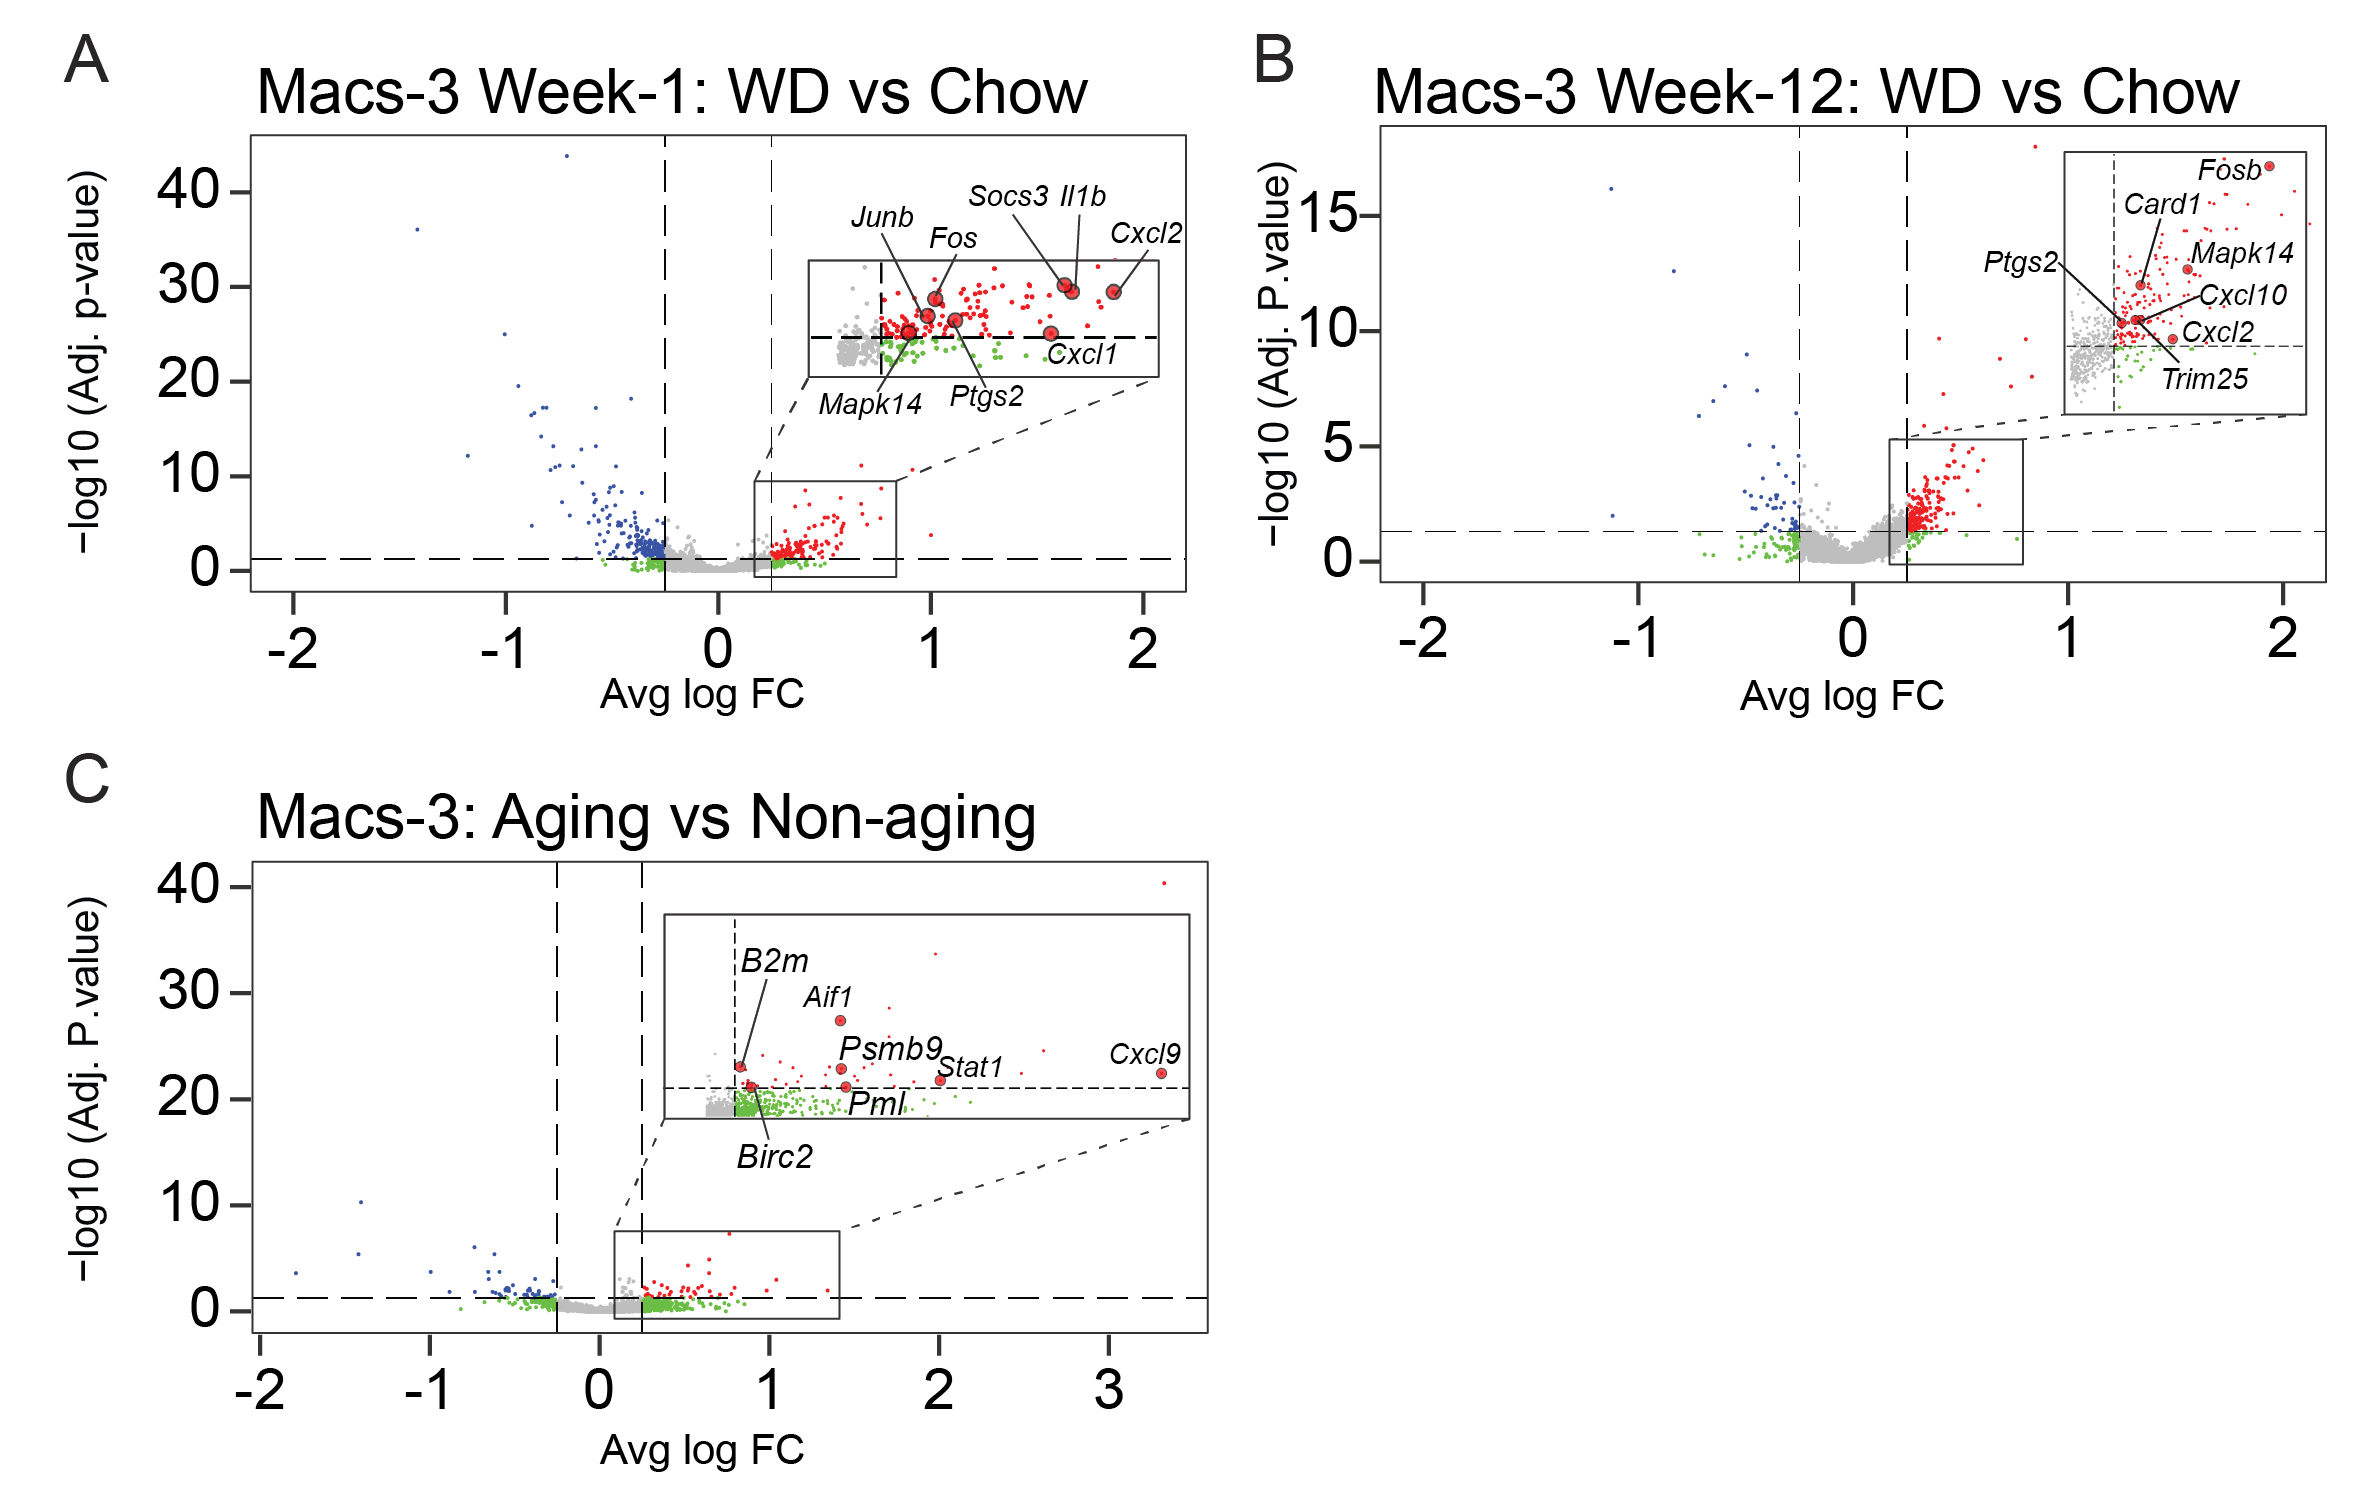
\includegraphics[width=\linewidth]{Chapter4/Fig/F2-11-01.png}
\caption[\glsentryshort{dge} analysis in Macs-3 macrophages]{\textbf{\gls{dge} analysis in Macs-3 macrophages.} \textbf{(A) - (C)} Volcano plots showing \gls{de} genes in Macs-3 sub-population, comparing \gls{wd} versus chow diet at Week-1 time-point \textbf{(A)}, \gls{wd} versus chow diet at Week-12 time-point \textbf{(B)} and chow diet-fed aging cohort versus chow diet-fed non-aging (W1 + W12) cohorts \textbf{(C)}. The dashed vertical lines represent $  \left|Avg. \log FC \right| $ = 0.25 and the dashed horizontal line represent $-\log_{10}(\num{0.05}) = 1.3$. Differentially up-regulated and down-regulated genes are depicted by red and blue dots respectively. Abbreviations: \gls{wd}, western diet; $Avg. \log\textsubscript{2} \glsentryshort{fc}$, $\log\textsubscript{2}$ \glsentrylong{fc} of the average expression of the gene between the two groups; Adj. p-value, adjusted p-value based on Bonferroni correction using all genes in the dataset.}
\label{fig:chp2_scrna_macrophages_macs3_dge}
\end{figure}

\par Consistent with the results from the \gls{dge} analysis \textbf{(\autoref{fig:chp2_scrna_macrophages_macs3_dge})}, Macs-3 did activate the type-1 \gls{ifn} response under both \gls{wd} and aging conditions. However, this response was notably intensified during aging (km-9). This heightened response is likely attributed to the enhanced canonical response and the absence of feedback inhibition by \textit{Stat3 / Socs3} \textbf{(\autoref{fig:chp2_scrna_macrophages_macs3_dge} A)}, which was observed in \gls{wd}. It might also be explained by the aging-specific attenuation of the \gls{perk} pathway (km-3), which has been proposed to maintain an immunosuppressive phenotype in macrophages \textbf{\cite{raines_perk_2022}}. Conversely, \gls{wd} feeding uniquely triggered the \gls{mtor} pathway (km-4) in Macs-3, further suggesting that it represents a non-canonical type-1 \gls{ifn} response \textbf{\cite{mazewski_type_2020}}. Furthermore, \gls{wd} feeding specifically triggered the activation of genes in the \gls{tnf}-$\alpha$ / \gls{nfkb} signaling pathway (km-6) in Macs-3, a change that was not evident during aging. This highlights the potential involvement of additional pro-inflammatory cytokines during metabolic stress as opposed to inflammaging.\\

\par Interestingly, despite Macs-2 exhibiting a lower activation profile compared to Macs-3, \gls{wd} feeding resulted in a stronger expression of genes coding for inflammatory cytokines and chemokines in Macs-2 \textbf{(\autoref{fig:app_scrna_macrophages_macs2_dge} A,B)}. In contrast, this induced up-regulation of cytokine genes observed in Macs-2 under \gls{wd} feeding conditions was not evident in the aging condition \textbf{(\autoref{fig:app_scrna_macrophages_macs2_dge} C)}. The Macs-2 macrophages also showed non-canonical type-1 \gls{ifn} responses, evident in the up-regulated \textit{Socs3} expression one week after starting the \gls{wd} feeding \textbf{(\autoref{fig:app_scrna_macrophages_macs2_dge} A)}. Intriguingly, the \gls{wd} triggered various inflammatory cytokine and chemokine gene expression, persisting twelve weeks into overnutrition \textbf{(\autoref{fig:app_scrna_macrophages_macs2_dge} B)}. In contrast, while Macs-2 in aging conditions exhibited signs of immune cell activation, it did not demonstrate cytokine expression \textbf{(\autoref{fig:app_scrna_macrophages_macs2_dge} C)}.\\


\begin{figure}[t]
\centering
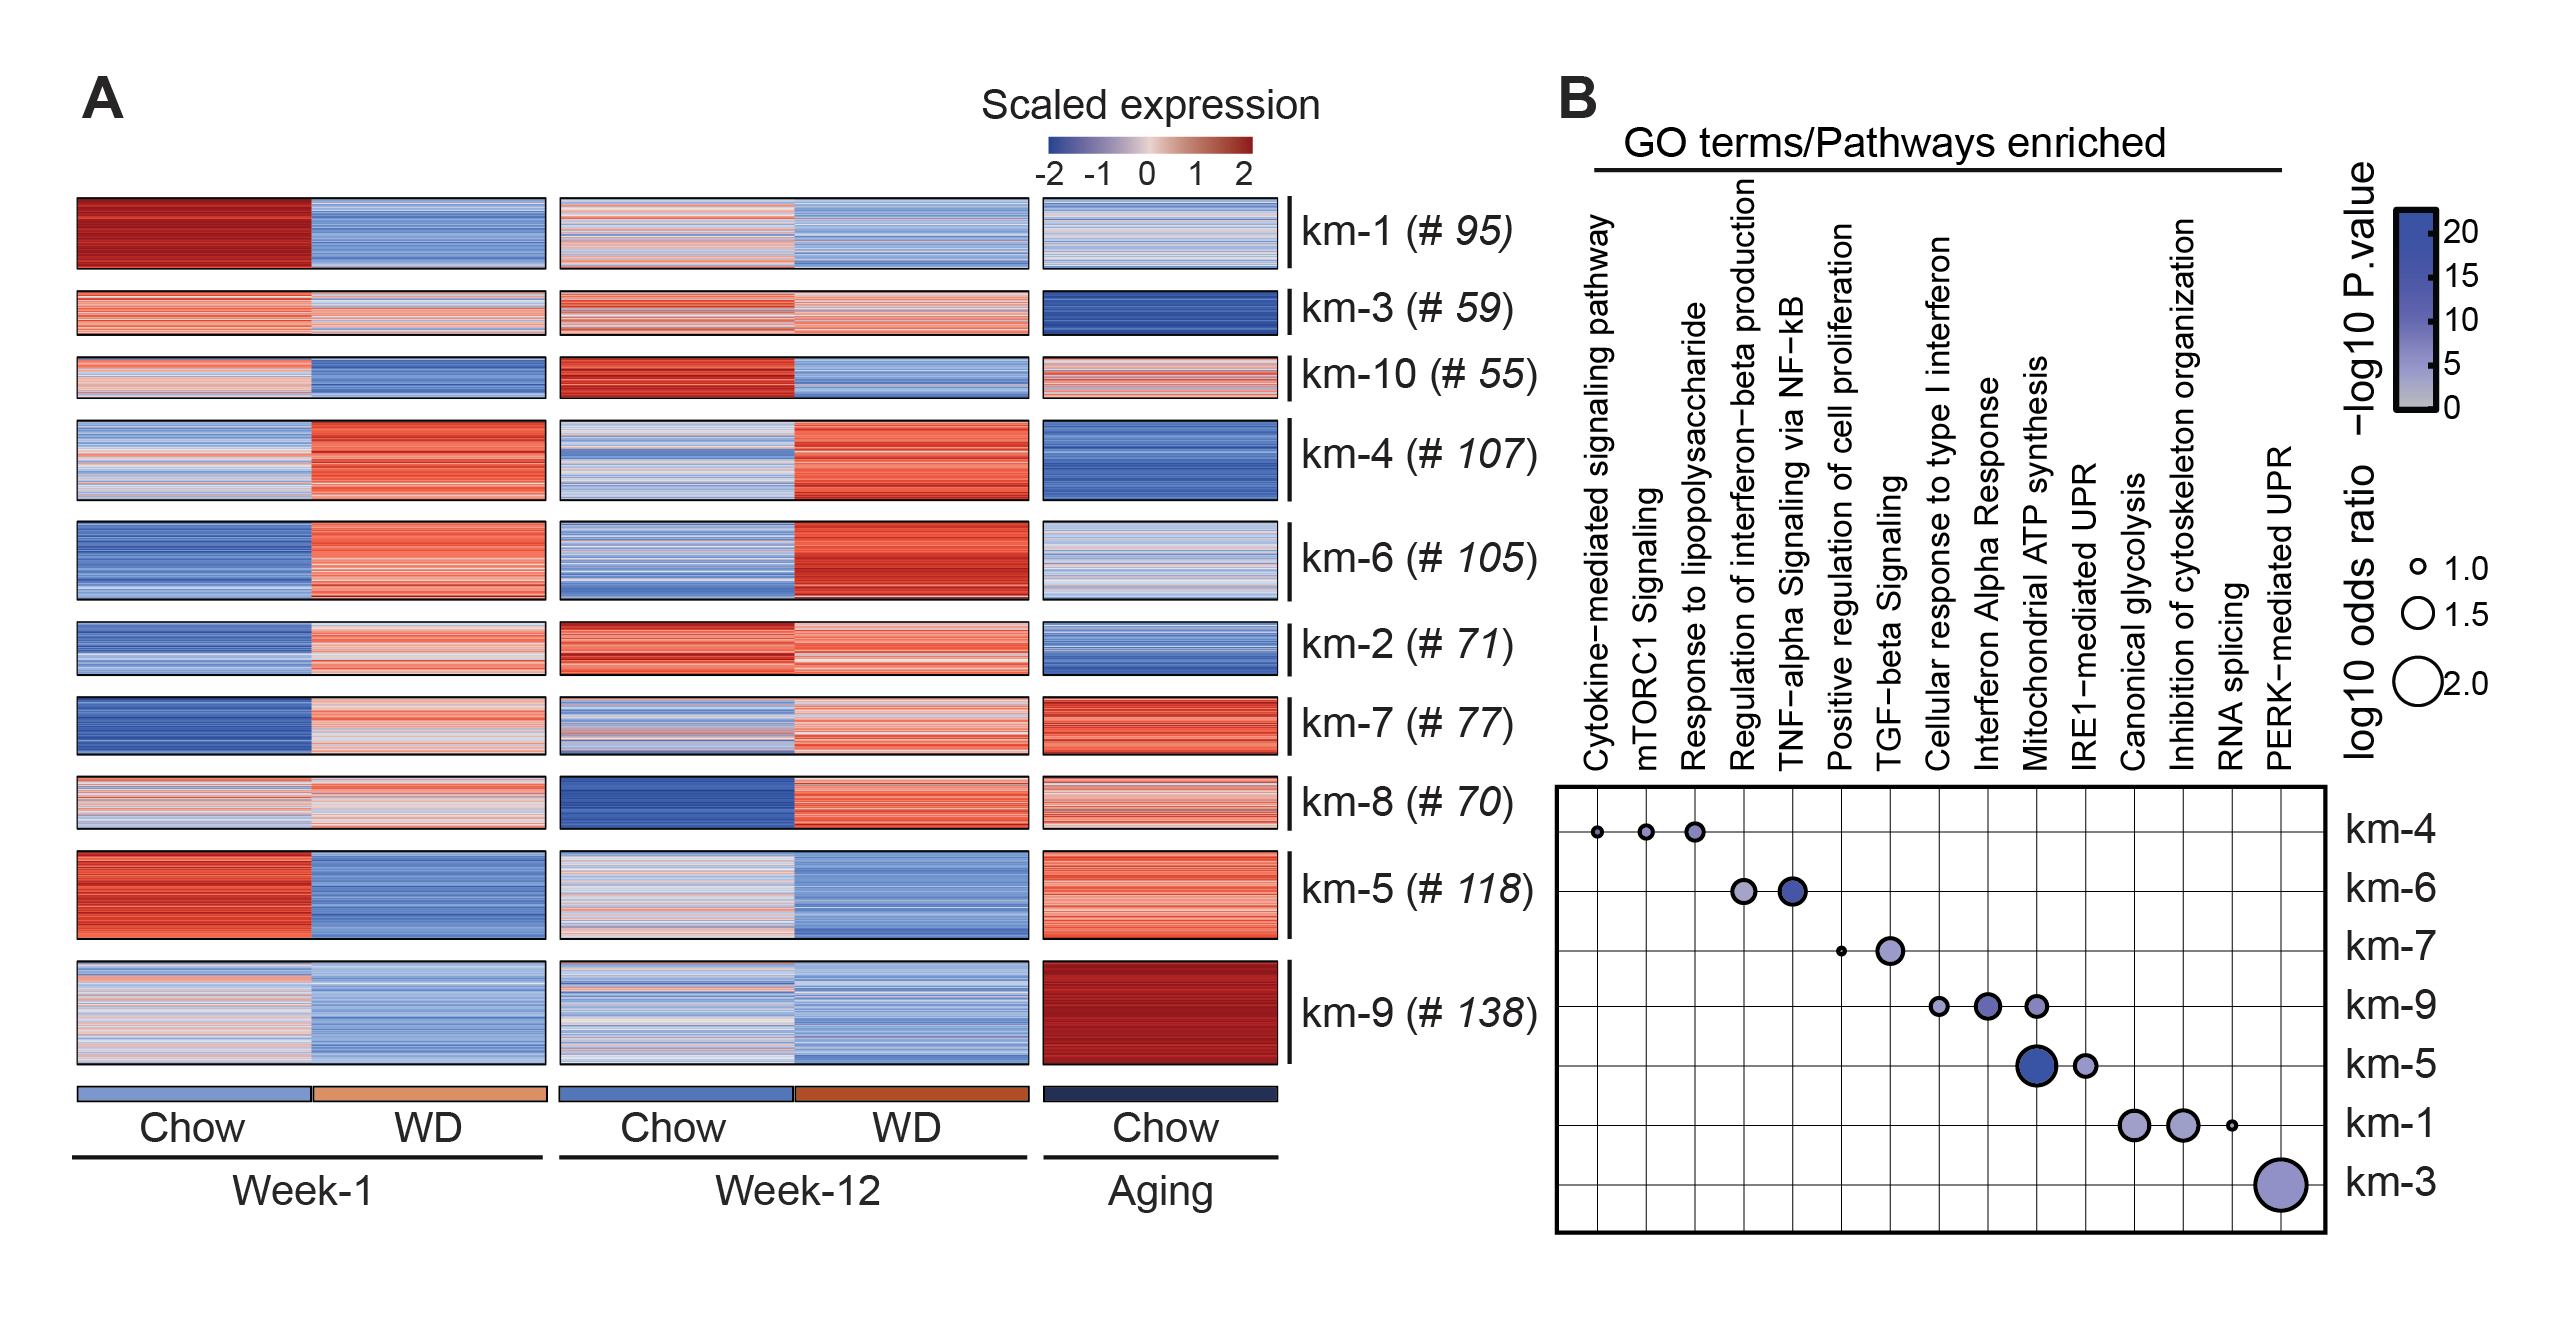
\includegraphics[width=\linewidth]{Chapter4/Fig/F2-11-02.png}
\caption[Expression patterns of \glsentryshort{de} genes in Macs-3 across overnutition and aging]{\textbf{Expression patterns of \gls{de} genes in Macs-3 across overnutition and aging.} \textbf{(A)} Heatmap depicting the scaled average expression of all 895 \gls{de} genes in Macs-3 sub-population across the experimental groups. The \gls{de} genes were clustered into 10 modules with \textit{k-means} clustering and are grouped by their modules in the heatmap. The number of genes in each \textit{k-means} module (km) is indicated in parantheses. \textbf{(B)} Dot plot depicting enriched \gls{go} terms or pathways in the selected modules from \textbf{(A)}. The color of the dots indicate the significance of the term in a particular module and the size of the dots correspond to odds ratio which measures the enrichment of overlapping genes between the modules and the annotated set relative to the expected random distribution.}
\label{fig:chp2_scrna_macrophages_macs3_clust}
\end{figure}

\par In summary, our analysis revealed an activation of the canonical type-1 \gls{ifn} response during inflammaging. While overnutrition can accelerate a similar process, it triggers a non-canonical signaling cascade thereby likely leading to a more pronounced inflammatory state.


\clearpage

\begin{comment}
    
\section[$\beta$-cells display distinct inflammatory profiles in response to obesity and aging]{$\beta$-cells display distinct inflammatory profiles in response\\to obesity and aging}
\label{sec:chp2_betacells}
Overnutrition and aging activate islet-associated macrophages, leading to varied inflammatory states in the islets. However, the response of pancreatic $\beta$-cells to these conditions, and how they might be affected by the altered inflammation, remains unclear. To explore this, we evaluated the metabolic phenotypes displayed by cohorts exposed to \gls{wd} and aging. Consistent with previous studies \textbf{\cite{}}, we noticed an acute islet dysfunction a week after initiating a \gls{wd} \textbf{(\autoref{fig:app_metab_betacells} A-D)}. Moreover, glucose intolerance and insulin resistance became noticeable after 12 weeks of overnutrition \textbf{(\autoref{fig:app_metab_betacells} E,F)}, coinciding with a compensatory rise in insulin secretion from the islets \textbf{(\autoref{fig:app_metab_betacells} G,H)}. Aging cohorts, however, retained normal glucose tolerance and insulin sensitivity \textbf{(\autoref{fig:app_metab_betacells} I,J)}, and their islets showed heightened insulin release under both basal and glucose-stimulated conditions in the \textit{in-vitro} culture \textbf{(\autoref{fig:app_metab_betacells} K,L)}.\\

%A critical facet of \gls{t2d} in $\beta$-cell dysfunction. However, the response of ... 
\par To characterize the islet $\beta$-cells, we further analyzed the $\beta$-cells derived from our \gls{scr} data. Following a sub-clustering analysis, we identified three $\beta$-cell sub-populations \textbf{(\autoref{fig:chp2_scrna_betacells1} A, \autoref{fig:app_scrna_betacells1} A)}. Compared to a previous single-cell analysis of 
murine islets \textbf{\cite{sachs_targeted_2020}} via label transfer \textbf{(\autoref{fig:app_scrna_betacells1} B)}, we observed that our $\beta$-3 sub-
population corresponded to the \textit{Cd81}\textsuperscript{+} immature $\beta$-cell sub-population \textbf{(\autoref{fig:app_scrna_betacells1} A, C)}. Whereas both $\beta$-1 and $\beta$-2 represented mature $\beta$-cells. $\beta$-1 exhibited enhanced \glslink{mtor}{mTORC1} signaling \textbf{(\autoref{fig:chp2_scrna_betacells1} B)} and $\beta$-2 displayed increased expression of genes involved in the peptide metabolic process \textbf{(\autoref{fig:chp2_scrna_betacells1} C)}. Unlike our observations in macrophages, the composition of the $\beta$-cell sub-populations remained highly stable under both \gls{wd} and aging conditions \textbf{(\autoref{fig:chp2_scrna_betacells1} E)}.\\

\begin{figure}[t!]
    \centering
    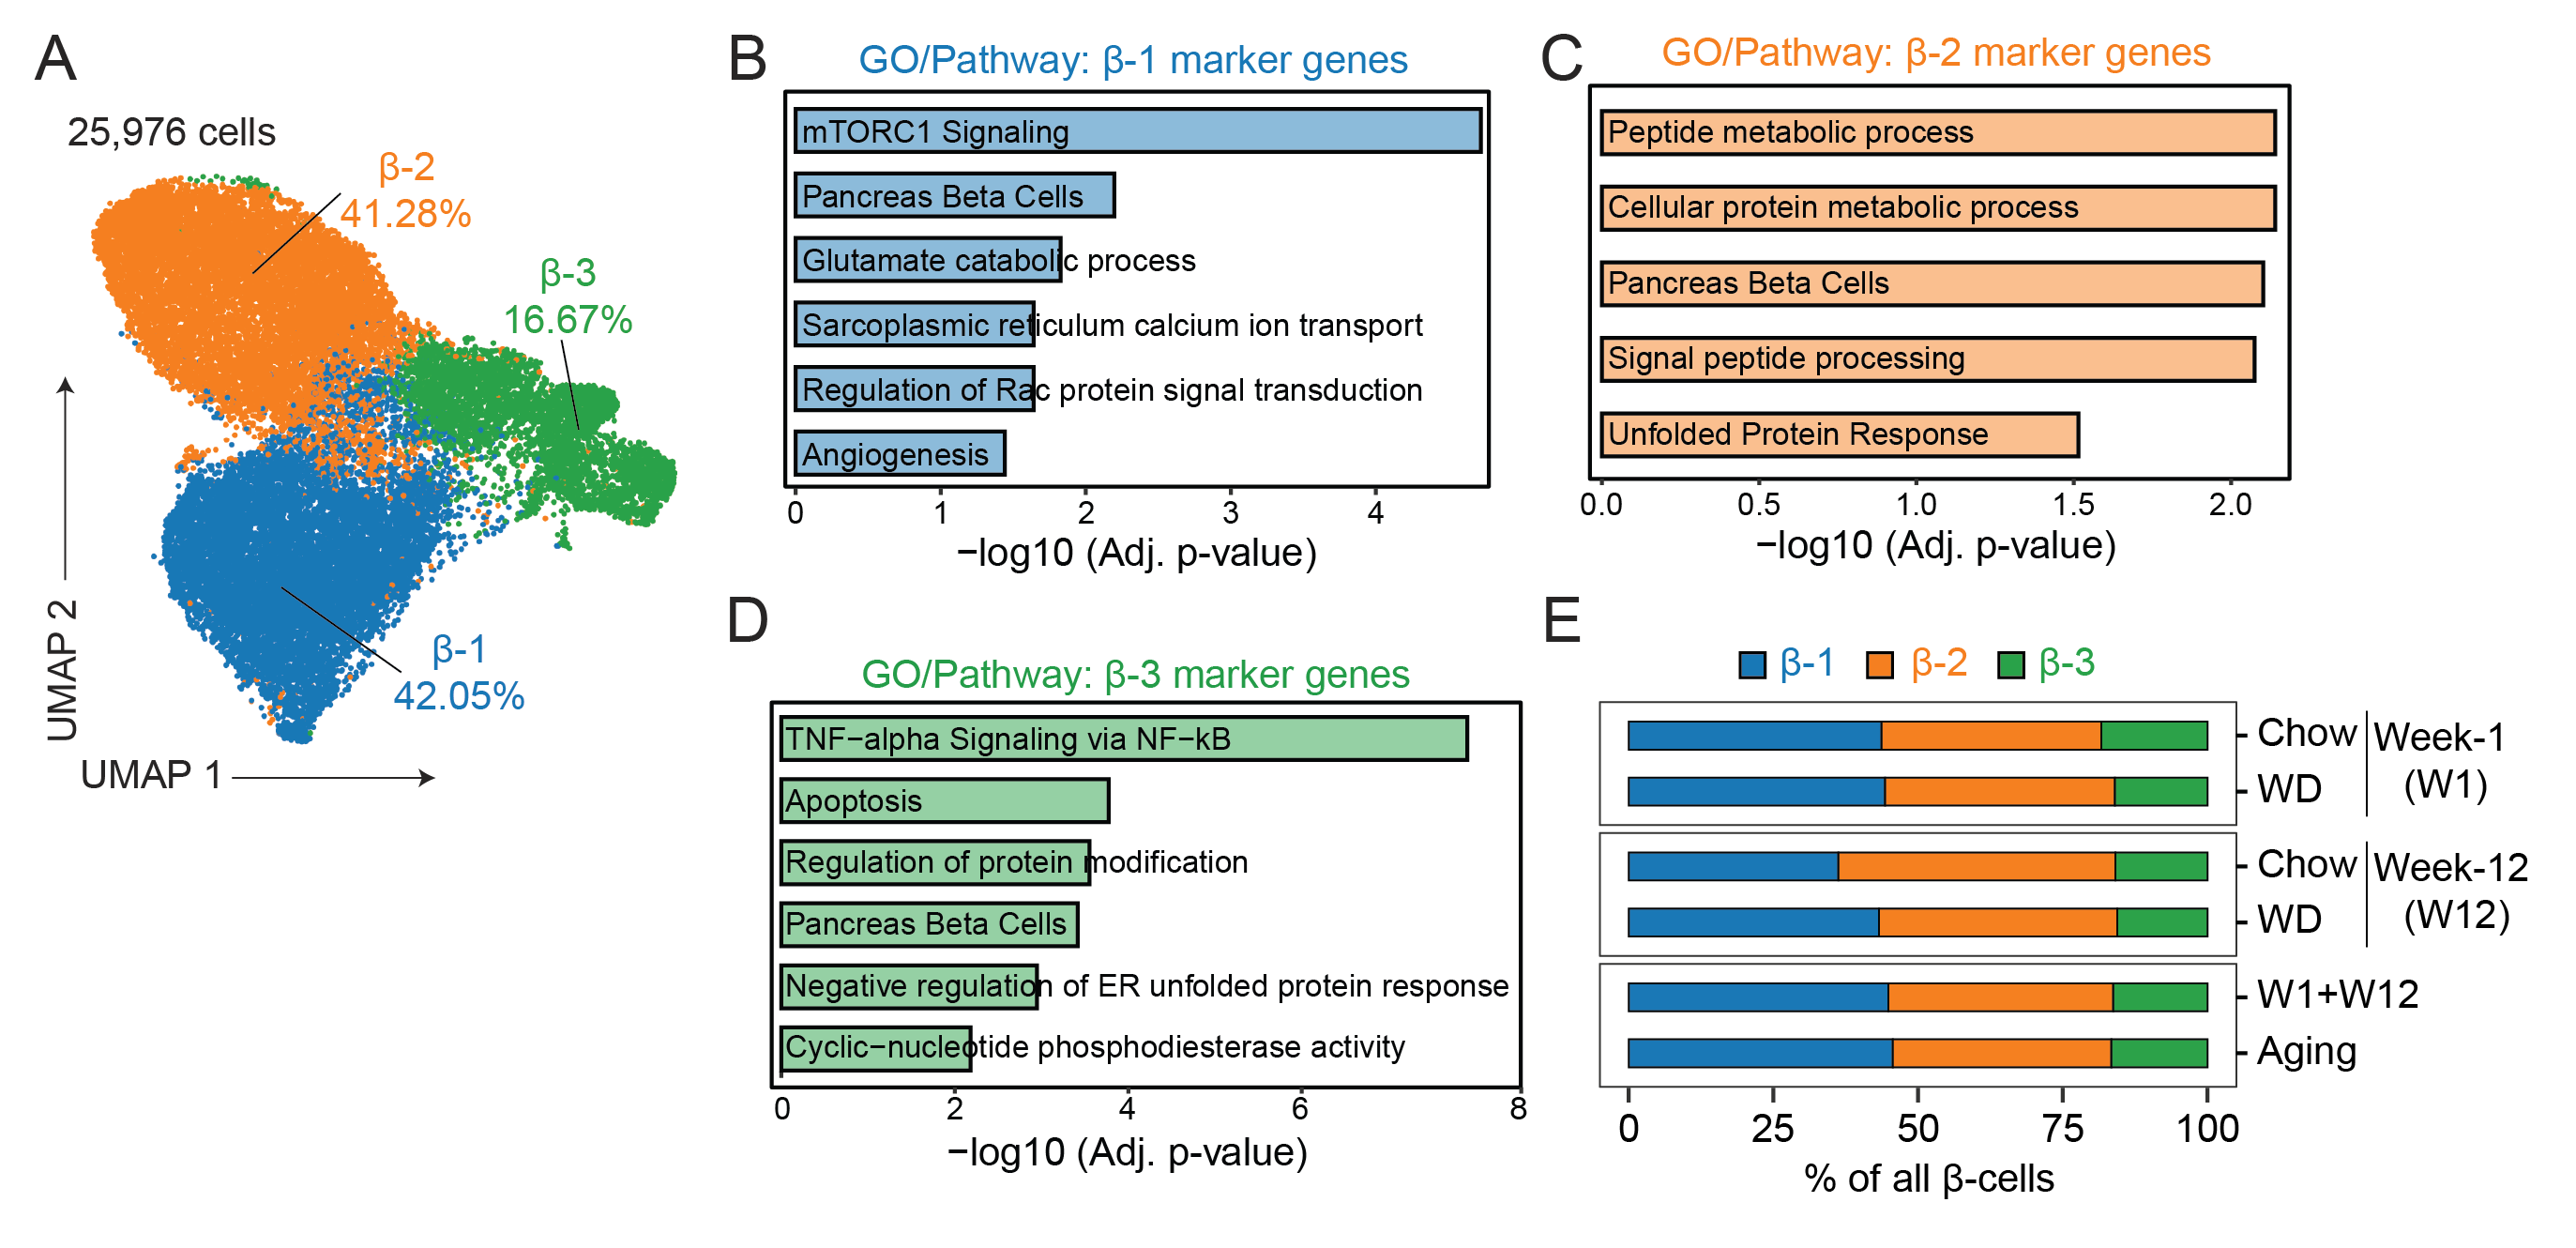
\includegraphics[width=\linewidth]{Chapter4/Fig/F2-12-02.png}
    \caption[Characterization of islet $\beta$-cells using \glslink{scr}{scRNA-seq}]{\textbf{Characterization of islet $\beta$-cells using \gls{scr}.} \textbf{(A)} \gls{umap} embedding of pancreatic islet $\beta$-cells, pooled from various experimental groups and replicates. Values indicate the overall proportion of each sub-population, defined based on marker gene expression. \textbf{(B-D)} Enriched \gls{go} terms among marker genes of $\beta$-1 \textbf{(B)}, $\beta$-2 \textbf{(C)} and $\beta$-3 \textbf{(D)}. Significance ($-\log_{10}$ adjusted p-value) of the enrichment are shown in bar plots. \textbf{(E)} The proportion of each $\beta$-cell sub-population in panel \textbf{(A)}, computed as a percentage of all $\beta$-cells in every experimental group. The cells from different biological replicate cohorts were pooled together.}
    \label{fig:chp2_scrna_betacells1}
\end{figure}
%\par Despite this, considerable changes in the transcriptome were observed across all β-cell sub-populations due to overnutrition and aging. 
\par To investigate the responses of islet $\beta$-cells to overnutrition and aging, we conducted a \gls{dge} analysis between \gls{wd} and chow diet fed cohorts after 1 and 12 weeks of feeding and between the chow diet fed aging cohort and the non-aging controls. Importantly, we observed that the three $\beta$-cell sub-populations responded similarly to \gls{wd} feeding and aging, as both, the direction and the magnitude of expression of the \gls{de} genes were similar across the three sub-populations \textbf{(\autoref{fig:app_scrna_betacells1} D-F)}. Based on these observations, we grouped all $\beta$-cells together, and re-performed the \gls{dge} analysis across all $\beta$-cells, identified 521 \gls{de} genes across all the experimental groups and clustered into gene modules \textbf{(\autoref{fig:chp2_scrna_betacells2} A)}. These modules encompass genes that display analogous expression patterns across overnutrition and aging conditions. Importantly, we identified modules that were unique to aging (km-9, km-10, and km-2), specific to \gls{wd} feeding (km-6, km-1, km-8, km-3, and km-7), or shared across both conditions (km-4 and km-5) \textbf{(\autoref{fig:chp2_scrna_betacells2} A)}. Through \gls{go} and pathway analysis \textbf{(\autoref{fig:chp2_scrna_betacells2} B)}, we found that overnutrition and aging typically boosted \glslink{oxphos}{OxPhos} (km-4), while concurrently weakening the expression of $\beta$-cell identity genes (km-5) \textbf{(\autoref{fig:chp2_scrna_betacells2} B)}. Changes exclusively linked to the \gls{wd} feeding involved a significant uptick in \gls{upr} (km-1, km-6 and km-8) and a distinct decline in genes linked to alternative splicing (km-3 and km-7) \textbf{(\autoref{fig:chp2_scrna_betacells2} B)}. Aging-related gene modules showed fewer enriched pathways likely due to fewer genes per module.\\ %We observed an aging-specific decrease in \textit{G6pc2} expression \textbf{(Fig. )} in β-cells, which is in line with their increased glucose sensitivity and enhanced insulin secretion at baseline glucose levels \textbf{(Fig. )}\\
\par Additionally, we identified genes activated by either acute (km-6) or chronic (km-8) \gls{wd} feeding. Specifically, the acute activation module (km-6), observed during 1 week of \gls{wd} feeding, was associated with \gls{tnf}-$\alpha$ pathway activation. Conversely, the chronic activation module (km-8), which was more evident after 12 weeks of \gls{wd} feeding, showed an up-regulation of genes linked to protein secretion. These findings indicate the a progression from islet dysfunction due to acute inflammatory response to compensatory insulin hypersecretion in response to prolonged metabolic stress  \textbf{(\autoref{fig:app_metab_betacells} D,H)}. Importantly, $\beta$-cells displayed a \gls{tnf}-$\alpha$ response after 1 week of \gls{wd} feeding, coinciding with an upsurge in \textit{Tnf} expression in Macs-2 in response to \gls{wd} feeding at the same time-point \textbf{(\autoref{fig:app_scrna_macrophages_macs2_dge} A)}.\\

\begin{figure}[t!]
    \centering
    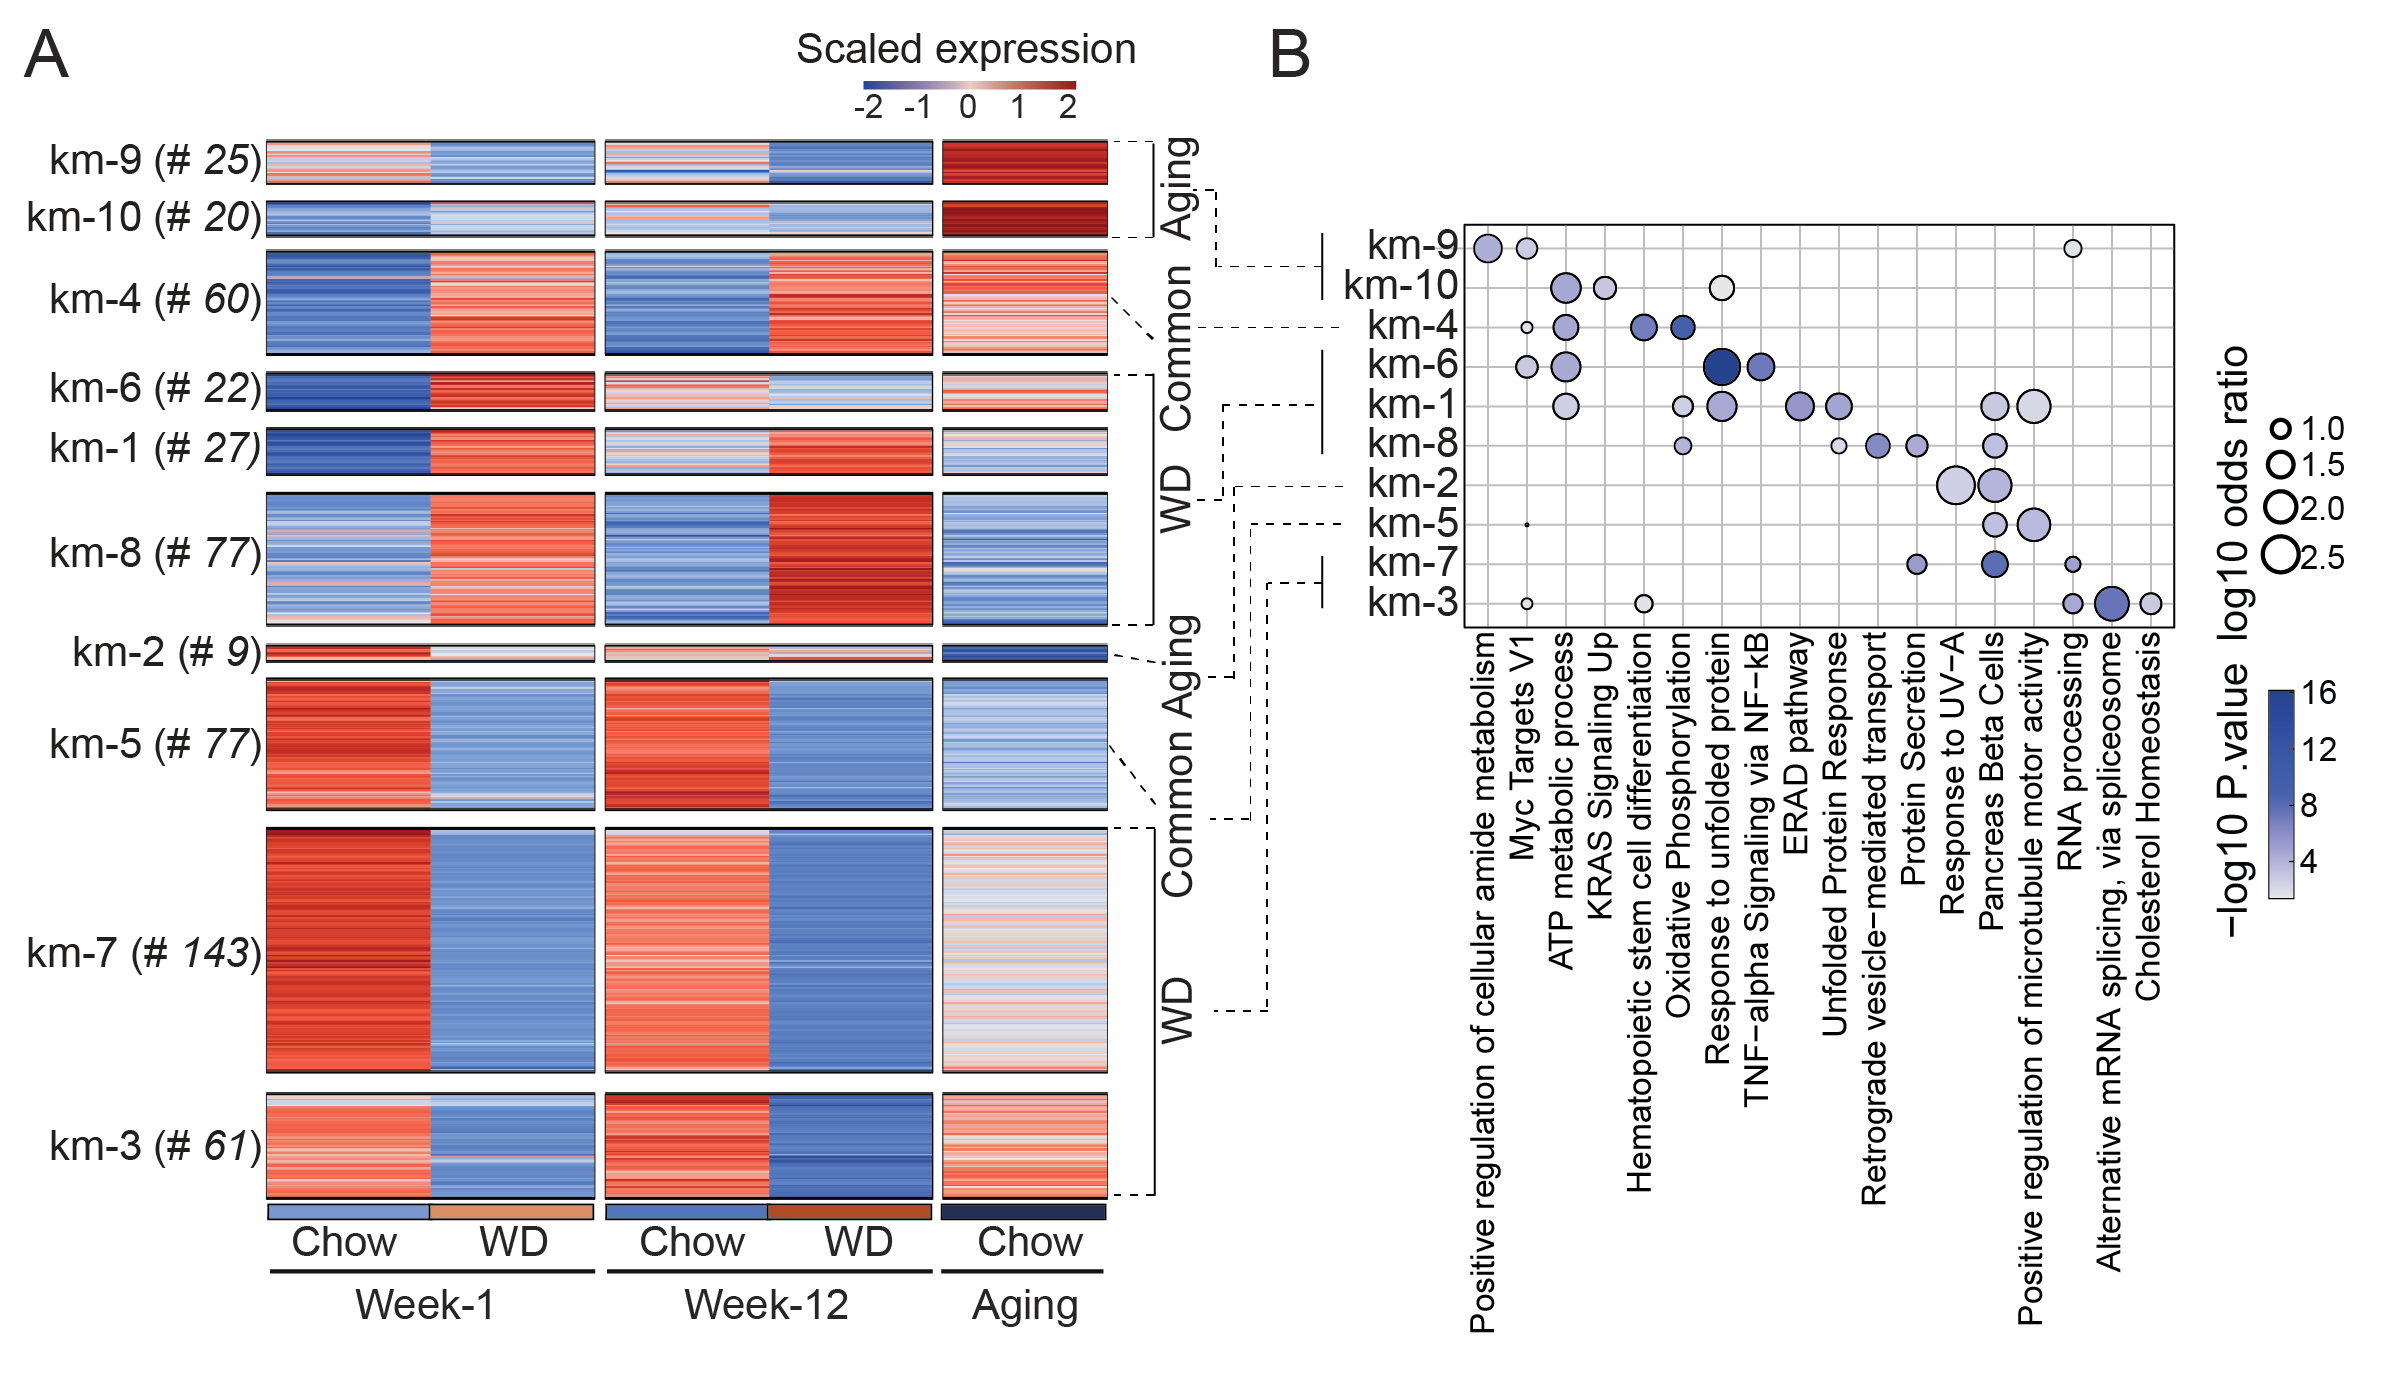
\includegraphics[width=\linewidth]{Chapter4/Fig/F2-12-01.png}
    \caption[\glslink{dge}{DGE} analayis in $\beta$-cells across \glslink{wd}{WD} feeding and aging]{\textbf{\gls{dge} analysis in $\beta$-cells across \gls{wd} feeding and aging.} \textbf{(A)} Heatmap depicting the scaled average expression of all \gls{de} genes in $\beta$-cells across the experimental groups (columns). The \gls{de} genes were clustered into 10 modules with the k-means clustering and are grouped by their modules in the heatmap (rows). \textbf{(B)} Dot plot depicting enriched \gls{go} terms or pathways in the selected modules from panel \textbf{(A)}. The color of the dots indicate the significance of the term in a particular module and the size of the dots correspond to odds ratio which measures the enrichment of overlapping genes between the modules and the annotated set relative to the expected random distribution. }
    \label{fig:chp2_scrna_betacells2}
\end{figure}

\par In conclusion, our analysis delineated the molecular responses of $\beta$-cells to \gls{wd} and aging established a possible link between $\beta$-cell transcriptomic profiles and the inflammatory environment dictated by islet-associated macrophages, offering insights into changes in $\beta$-cell function in response to overnutition and aging.

%\clearpage

\end{comment}

%\clearpage

\section[Metabolic stress accelerates aging-induced accumulation of CD8\textsuperscript{+} cytotoxic T-cells in the pancreas]{Metabolic stress accelerates aging-induced accumulation\\of CD8\textsuperscript{+} cytotoxic T-cells in the pancreas}
\label{sec:sc_tcells}

While there has been considerable focus on the role of islet macrophages during obesity-induced islet inflammation, research on adaptive immune components, particularly T-cells is less common due to their low numbers within the islets, thereby making their detailed characterization more challenging. The immune cell focused \gls{imc} panel \textbf{(\autoref{tab:app_imc_panel})} allowed us to characterize the T-cell populations in the pancreatic tissue in great detail. Our \gls{imc} analysis revealed an increase in pancreatic T-cells during both overnutrition and aging conditions \textbf{(\autoref{fig:chp2_imc_tcells1} A)}. In particular, we observed an expansion of CD8\textsuperscript{+} activated effector-like T-cells in the pancreas, which was more pronounced under \gls{wd} feeding \textbf{(\autoref{fig:chp2_imc_tcells1} B,D)}. However, similar to the previously observed variability in the F4/80\textsuperscript{\textit{low}} macrophage population \textbf{(\autoref{fig:chp2_imc_macrophages2} A,} middle\textbf{)}, the 


\begin{figure}[b!]
\centering
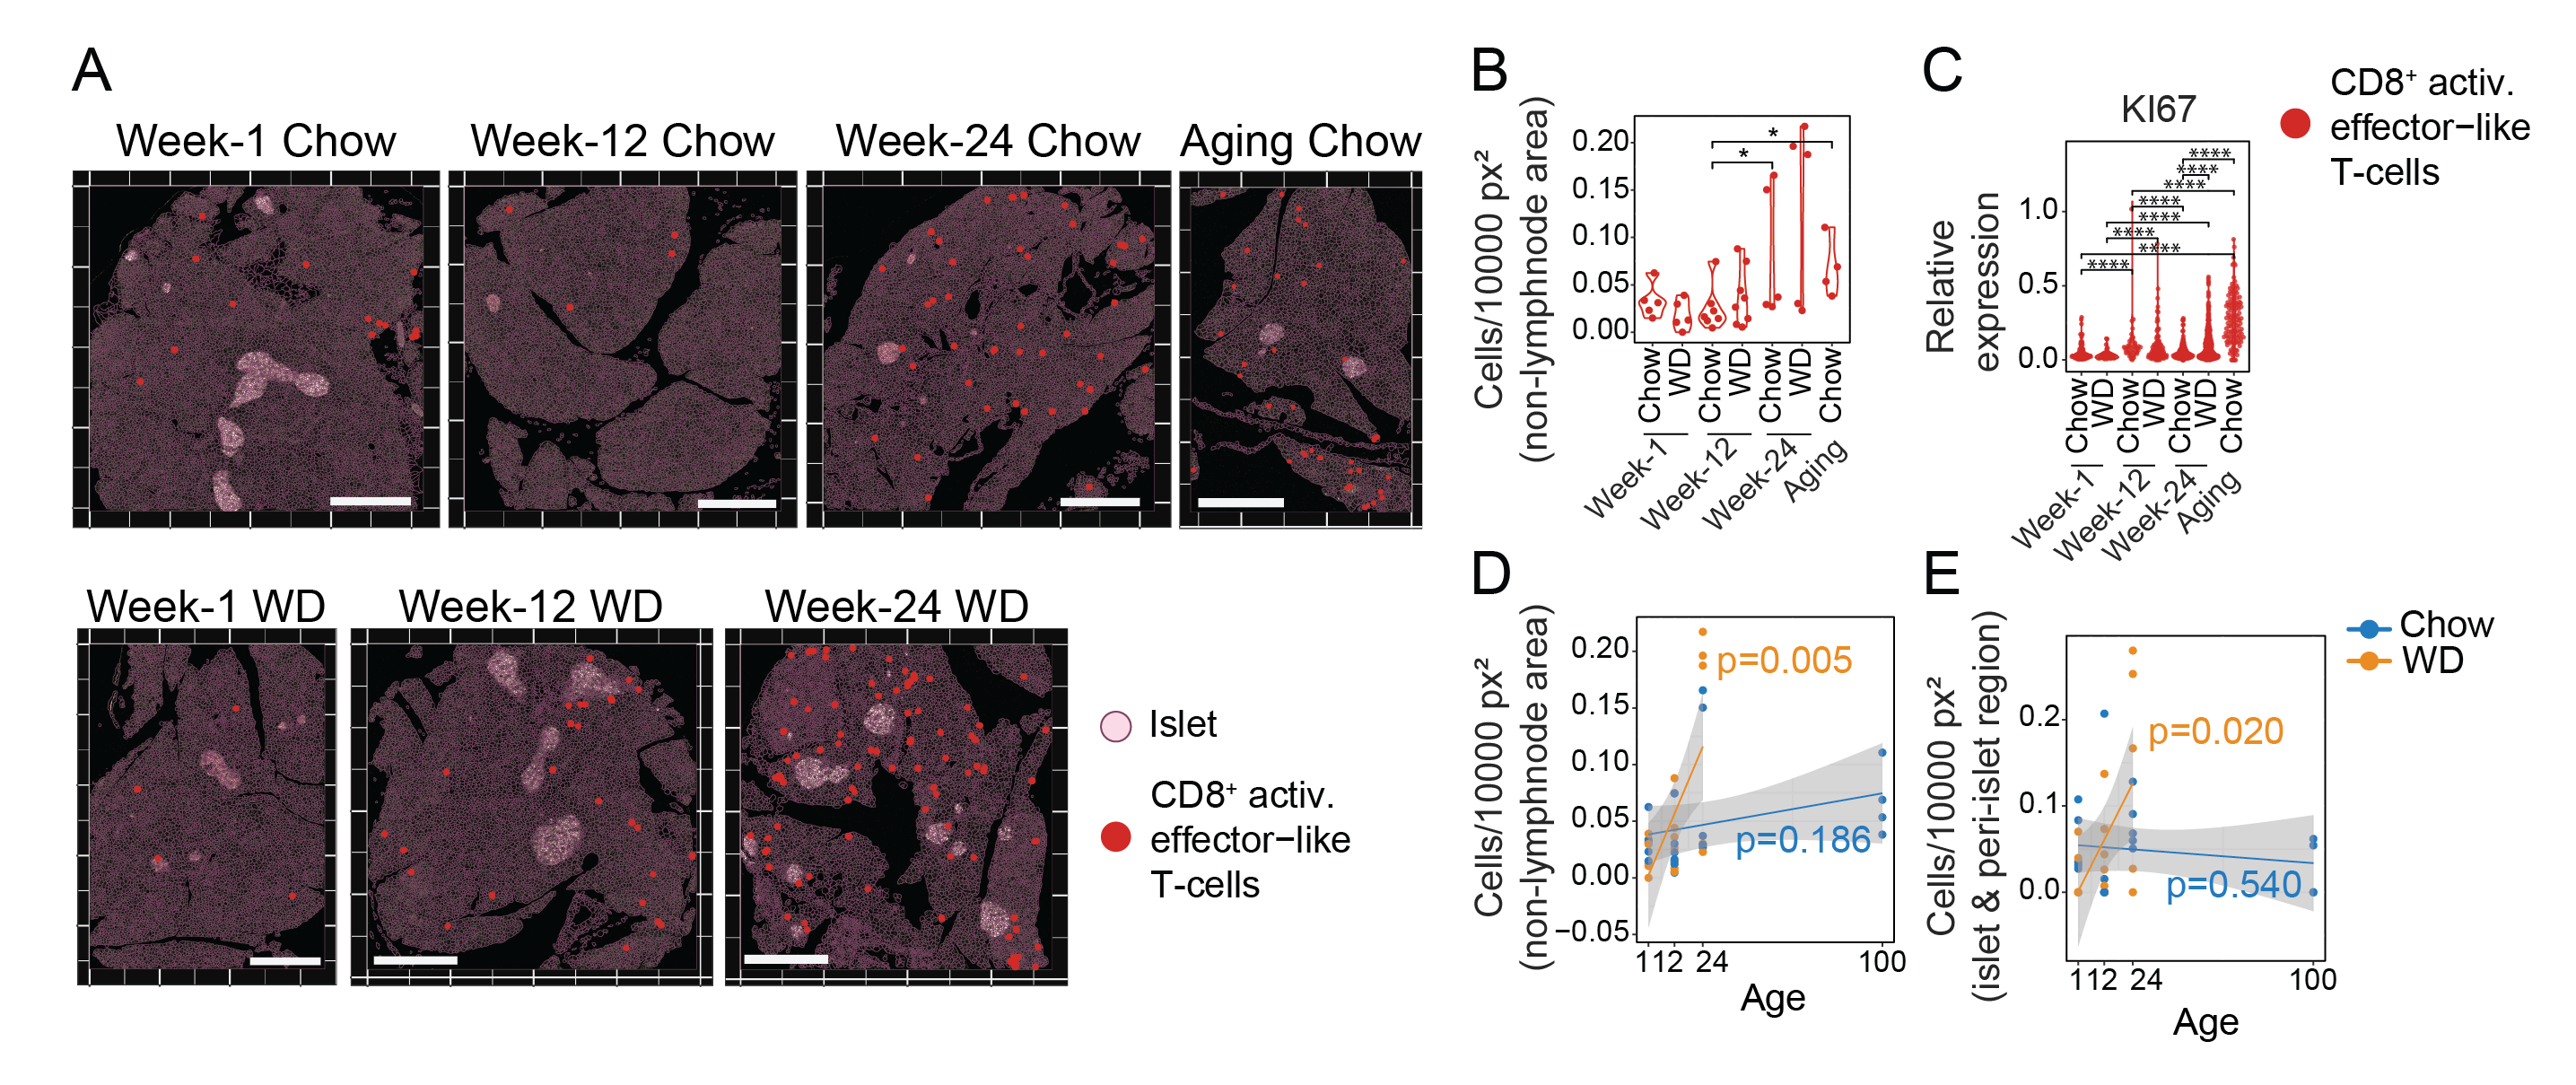
\includegraphics[width=\linewidth]{Chapter4/Fig/F2-10-02.png}
\caption[Accelerated accumulation of CD8\textsuperscript{+} cytotoxic T-cells in pancreas]{\textbf{Accelerated accumulation of CD8\textsuperscript{+} cytotoxic T-cells in pancreas in response to \gls{wd} feeeding.} \textbf{(A)} Representative \glspl{roi} showing CD8\textsuperscript{+} activated effector-like T-cells in the pancreas. Pancreatic islet regions are marked by raw INS signal (white).  Scale bar 500 \textmu m. \textbf{(B)} Violin plot displaying the densities of CD8\textsuperscript{+} activated effector-like T-cells in non-lymph node pancreatic regions, presented for each mouse across various experimental conditions. \textbf{(C)} Violin plot depicting \textit{arcsinh} transformed KI67 channel expression of CD8\textsuperscript{+} activated effector-like T cells across experimental groups. \textbf{(D) - (E)} Scatter plot depicting the density of CD8\textsuperscript{+} activated effector-like T-cells in the pancreas \textbf{(D)} and in the pancreatic islet and peri-islet regions \textbf{(E)} across experimental groups. Linear regression fits representing the cell density trends over time are plotted as solid lines. The 95\% confidence intervals for each linear regression are highlighted in grey. $\textsuperscript{*} p < 0.05, \textsuperscript{**} p < 0.01, \textsuperscript{***} p < 0.001, \textsuperscript{***} p < 0.0001$. P-values were calculated using the Wilcoxon rank-sum test with Bonferroni correction. \textit{This data and figure were originally generated by Dr. Matthias Barone and reused here with permission.}}
\label{fig:chp2_imc_tcells1}
\end{figure}

\clearpage

\gls{wd} feeding also resulted in high variability in the dynamics of this T-cell population. In line with these observations, we found elevated levels of KI67 channel expression within these T-cells under both overnutrition and aging conditions \textbf{(\autoref{fig:chp2_imc_tcells1} C)}. This led us to question whether these CD8\textsuperscript{+} activated effector-like T-cells are further recruited to the pancreatic islets under metabolic and age-induced stress. To investigate this, we analyzed the cell density within the islets and their peripheral regions. We observed significant enrichment of CD8\textsuperscript{+} activated effector-like T-cells in the peri-islet regions under \gls{wd} conditions, but not during aging \textbf{(\autoref{fig:chp2_imc_tcells1} E)}.\\

%\clearpage

\par The CD45 enrichment approach allowed us to recover a considerable proportion of T-cells from within the pancreatic islets. To gain deeper insights into the dynamics of T-cell sub-populations within the pancreatic islets, we conducted a sub-clustering analysis of our single-cell data, including the total cellular space of non-B-cell lymphocytes (T-cells \& others in \textbf{\autoref{fig:chp2_fullscRNA} B}). We identified several different T-cell sub-populations, together with other lymphocytes such as \glspl{ilc} -  \gls{ilc}2 and \gls{ilc}3 and \gls{nk} cells \textbf{(\autoref{fig:chp2_scrna_tcells1} A,C; \autoref{fig:app_scrna_tcells1} C,D)}. %It is noteworthy that the major T-cell sub-populations identified within the pancreatic islets from single-cell data mirrored those observed in the whole pancreas from \gls{imc} analysis.  
Based on marker expression, we identified  CD8\textsuperscript{+} cytotoxic T-cells, CD8\textsuperscript{+} memory T-cells, and \gls{treg} within the islets \textbf{(\autoref{fig:app_scrna_tcells1})}. These subsets exhibited a strong phenotypic alignment with the CD8\textsuperscript{+} activated effector-like T-cells, CD4\textsuperscript{+} / CD8\textsuperscript{+} memory-like cells, and \gls{treg} defined in our \gls{imc} data respectively \textbf{(\autoref{fig:app_scrna_tcells1} A,B)}. The precise correlation was underscored by their characteristic expression of EOMES (\textit{Eomes}), CD127 (\textit{Il7r}) and FOXP3 (\textit{Foxp3}), respectively \textbf{(\autoref{fig:app_scrna_tcells1} A,B)}. The whole transcriptome analysis revealed additional marker genes in the CD8\textsuperscript{+} cytotoxic T-cells, such \textit{Gzmk} (granzyme) and \textit{Ccl5} \textbf{(\autoref{fig:chp2_scrna_tcells1} C)}. Interestingly, similar to the CD8\textsuperscript{+} activated effector-like T-cells seen in the \gls{imc} data, the islet-associated CD8\textsuperscript{+} cytotoxic T-cells identified in the \gls{scr} data also expanded in response to \gls{wd} feeding \textbf{(\autoref{fig:chp2_scrna_tcells1} B)}. Moreover,this expansion was significant during aging within the islets in the \gls{scr} data \textbf{(\autoref{fig:chp2_scrna_tcells1} B)} compared to previous \gls{imc} analyses \textbf{(\autoref{fig:chp2_imc_tcells1} E)}.\\

\par Additionally, our \gls{scr} analysis provided increased resolution in identifying T-cell sub-populations within pancreatic islets, distinguishing two distinct sub-populations of naive T-cells marked by CD4 and CD8 \textbf{(\autoref{fig:chp2_scrna_tcells1} A,C; \autoref{fig:app_scrna_tcells1} C)}. These correspond to a single CD4\textsuperscript{+}/CD8\textsuperscript{+} non-proliferative, silent T-cell sub-population in our \gls{imc} data, characterized by high CD127 and low KI67 protein expression \textbf{(\autoref{fig:app_scrna_tcells1} A)}. We further revealed additional rare T-cell sub-populations within the islet, including Th1-like, Tfh-like, Naive-translation T-cells, \gls{ifn}-responsive T-cells, and a subset of $\gamma\delta$ T-cells \textbf{(\autoref{fig:chp2_scrna_tcells1} A,C; \autoref{fig:app_scrna_tcells1} C,D)}.\\


% The whole transcriptomic analysis further augmented our resolution in detecting islet-associated T-cell sub-populations. Notably, we identified two distinct naive T-cell sub-populations, each manifesting differential CD4 and CD8 expression profiles \textbf{(\autoref{fig:chp2_scrna_tcells1} A,C; \autoref{fig:app_scrna_tcells1} C)}. This observation correlates with the mixed CD4\textsuperscript{+}/CD8\textsuperscript{+} non-proliferative silent T-cell cluster defined in our \gls{imc} data, which was also characterised by high CD127 but low KI67 protein expression (\textbf{Supp. Fig.\ref{FIG} A}). Both, the \gls{scr} and \gls{imc} analyses (\textbf{Fig.\ref{fig2-10} H} and \textbf{Supp. Fig.\ref{FIG} A}) revealed highest EOMES/\textit{Eomes} expression for the CD8\textsuperscript{+} cytotoxic / activated effector-like T-cells. The cytotoxic T-cell subpopulation in the single-cell data was also characterized by high expression of granzyme K (\textit{Gzmk}) and chemokine ligand 5 \textit{Ccl5} (\textbf{Fig.\ref{fig2-10} H}).

\begin{figure}[t!]
\centering
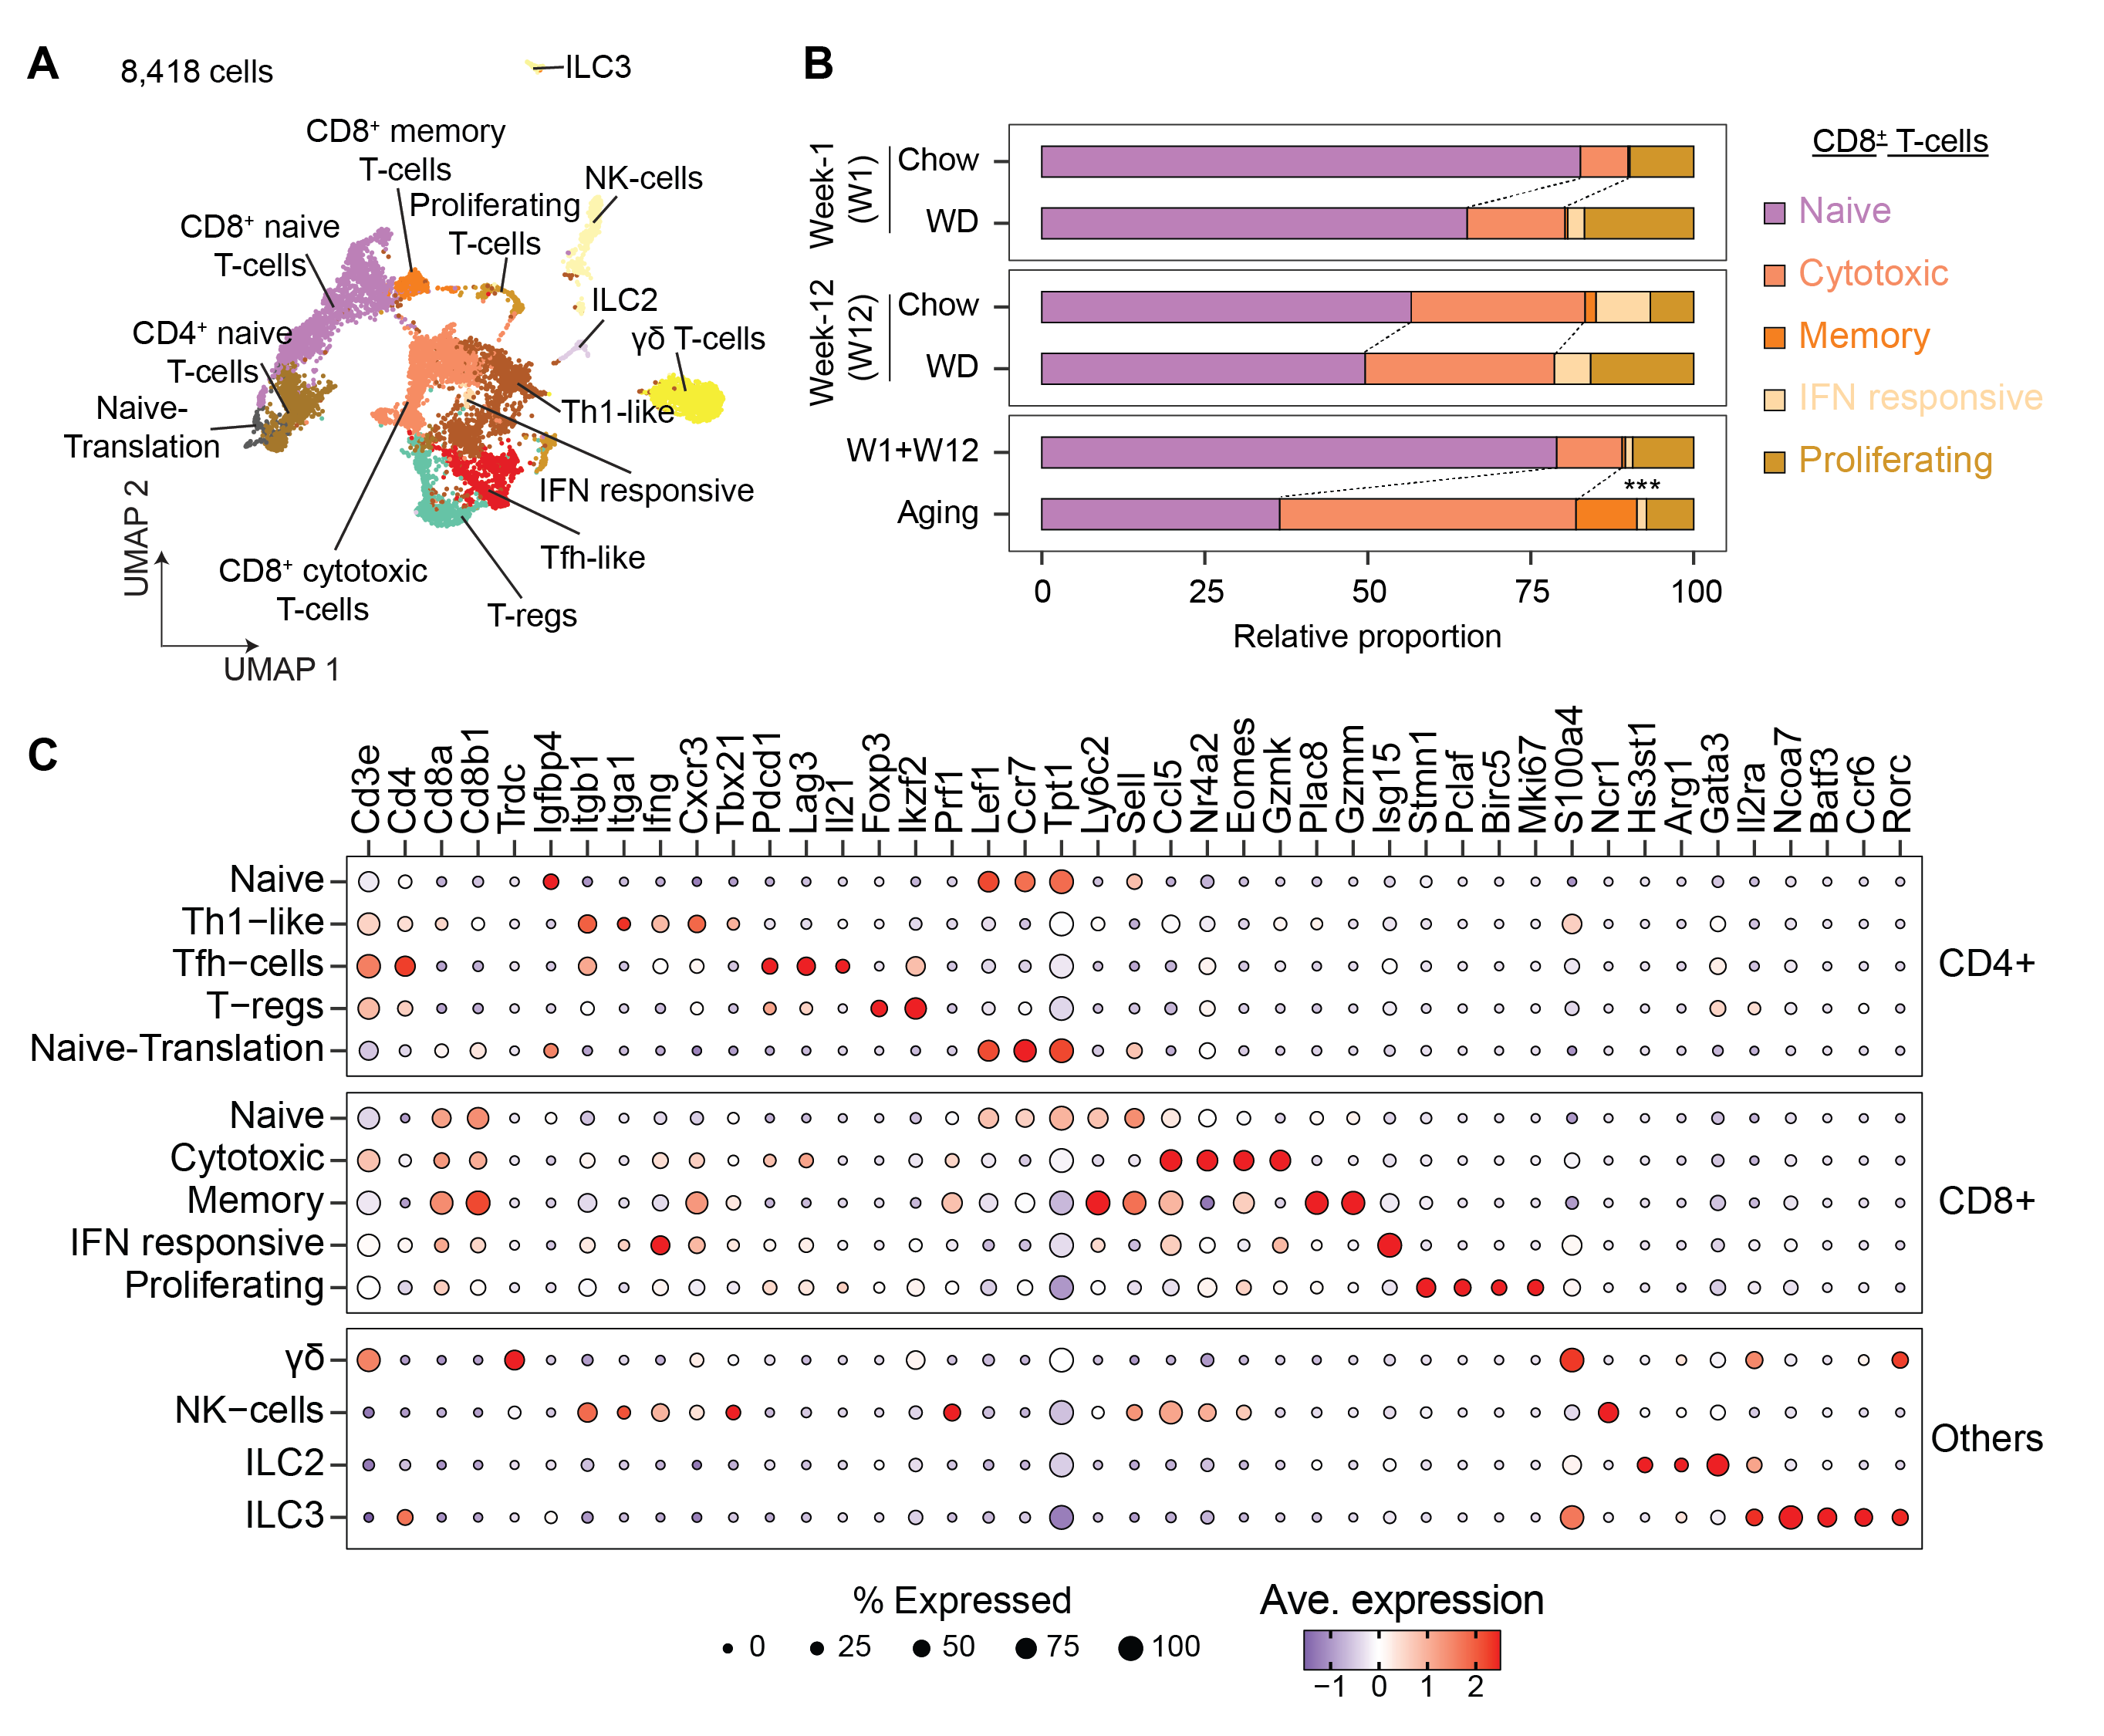
\includegraphics[width=\linewidth]{Chapter4/Fig/F2-10-01.png}
\caption[Characterization of T-cell sub-populations in \glsentryshort{scr} data]{\textbf{Characterization of islet-associated T-cell sub-populations in \gls{scr} data.} \textbf{(A)} \gls{umap} embedding of islet-associated T- and other lymphocyte sub-populations pooled across all experimental groups. Cell -ypes were defined based on marker gene expression. \textbf{(B)} The proportion of each CD8\textsuperscript{+} T-cell sub-population in \textbf{(A)}, computed as a percentage of all CD8\textsuperscript{+} cells in every experimental group. The cells from different biological replicate cohorts were pooled together. *: p<0.05, **: p<0.01, ***: p<0.001. p values were calculated from a mixed-effects binomial model. \textbf{(C)} Dot plot depicting hallmark genes for all annotated T- and other lymphocyte sub-populations in \textbf{(A)}. The color of the dots represent the scaled average expression of the genes and the size of the dots correspond to the percentage of cells expressing the gene.
}
\label{fig:chp2_scrna_tcells1}
\end{figure}

\par Collectively, combining \gls{imc} and single-cell analysis, we have provided a comprehensive portrayal of T-cells within the pancreas, elucidating their population dynamics in both the exocrine and endocrine compartments under overnutrition and aging conditions. Key observations included an aging-induced expansion of \textit{Eomes} expressing CD8\textsuperscript{+} cytotoxic T-cells, both in the pancreas and the islets, which was accelerated by metabolic stress.

%\clearpage

\section[CD8\textsuperscript{+} cytotoxic T-cells receive signals from \glsentryshort{ifn}-activated macrophages]{CD8\textsuperscript{+} cytotoxic T-cells receive signals from \gls{ifn}-activated\\macrophages}
\label{sec:chp2_cell_cell}

Under metabolic stress, we observed a metabolic stress-induced enhanced accumulation of type-1 \gls{ifn} responsive inflammatory macrophages within the islets in our \gls{scr} data \textbf{(\autoref{fig:chp2_scrna_macrophages} D)} and CD8\textsuperscript{+} activated-effector like T-cells in the peri-islet regions \textbf{(\autoref{fig:chp2_imc_tcells1} E)}. As activated macrophages can elicit T-cell stimulatory signals, we investigated their inter-cellular communication potential by performing \gls{lri} analysis (see \hyperref[subsubsec:met_chp2_cellcell]{\textbf{Methods}}).

\subsubsection{\large Intercellular interactions under acute overnutrition}


\begin{figure}[b!]
\centering
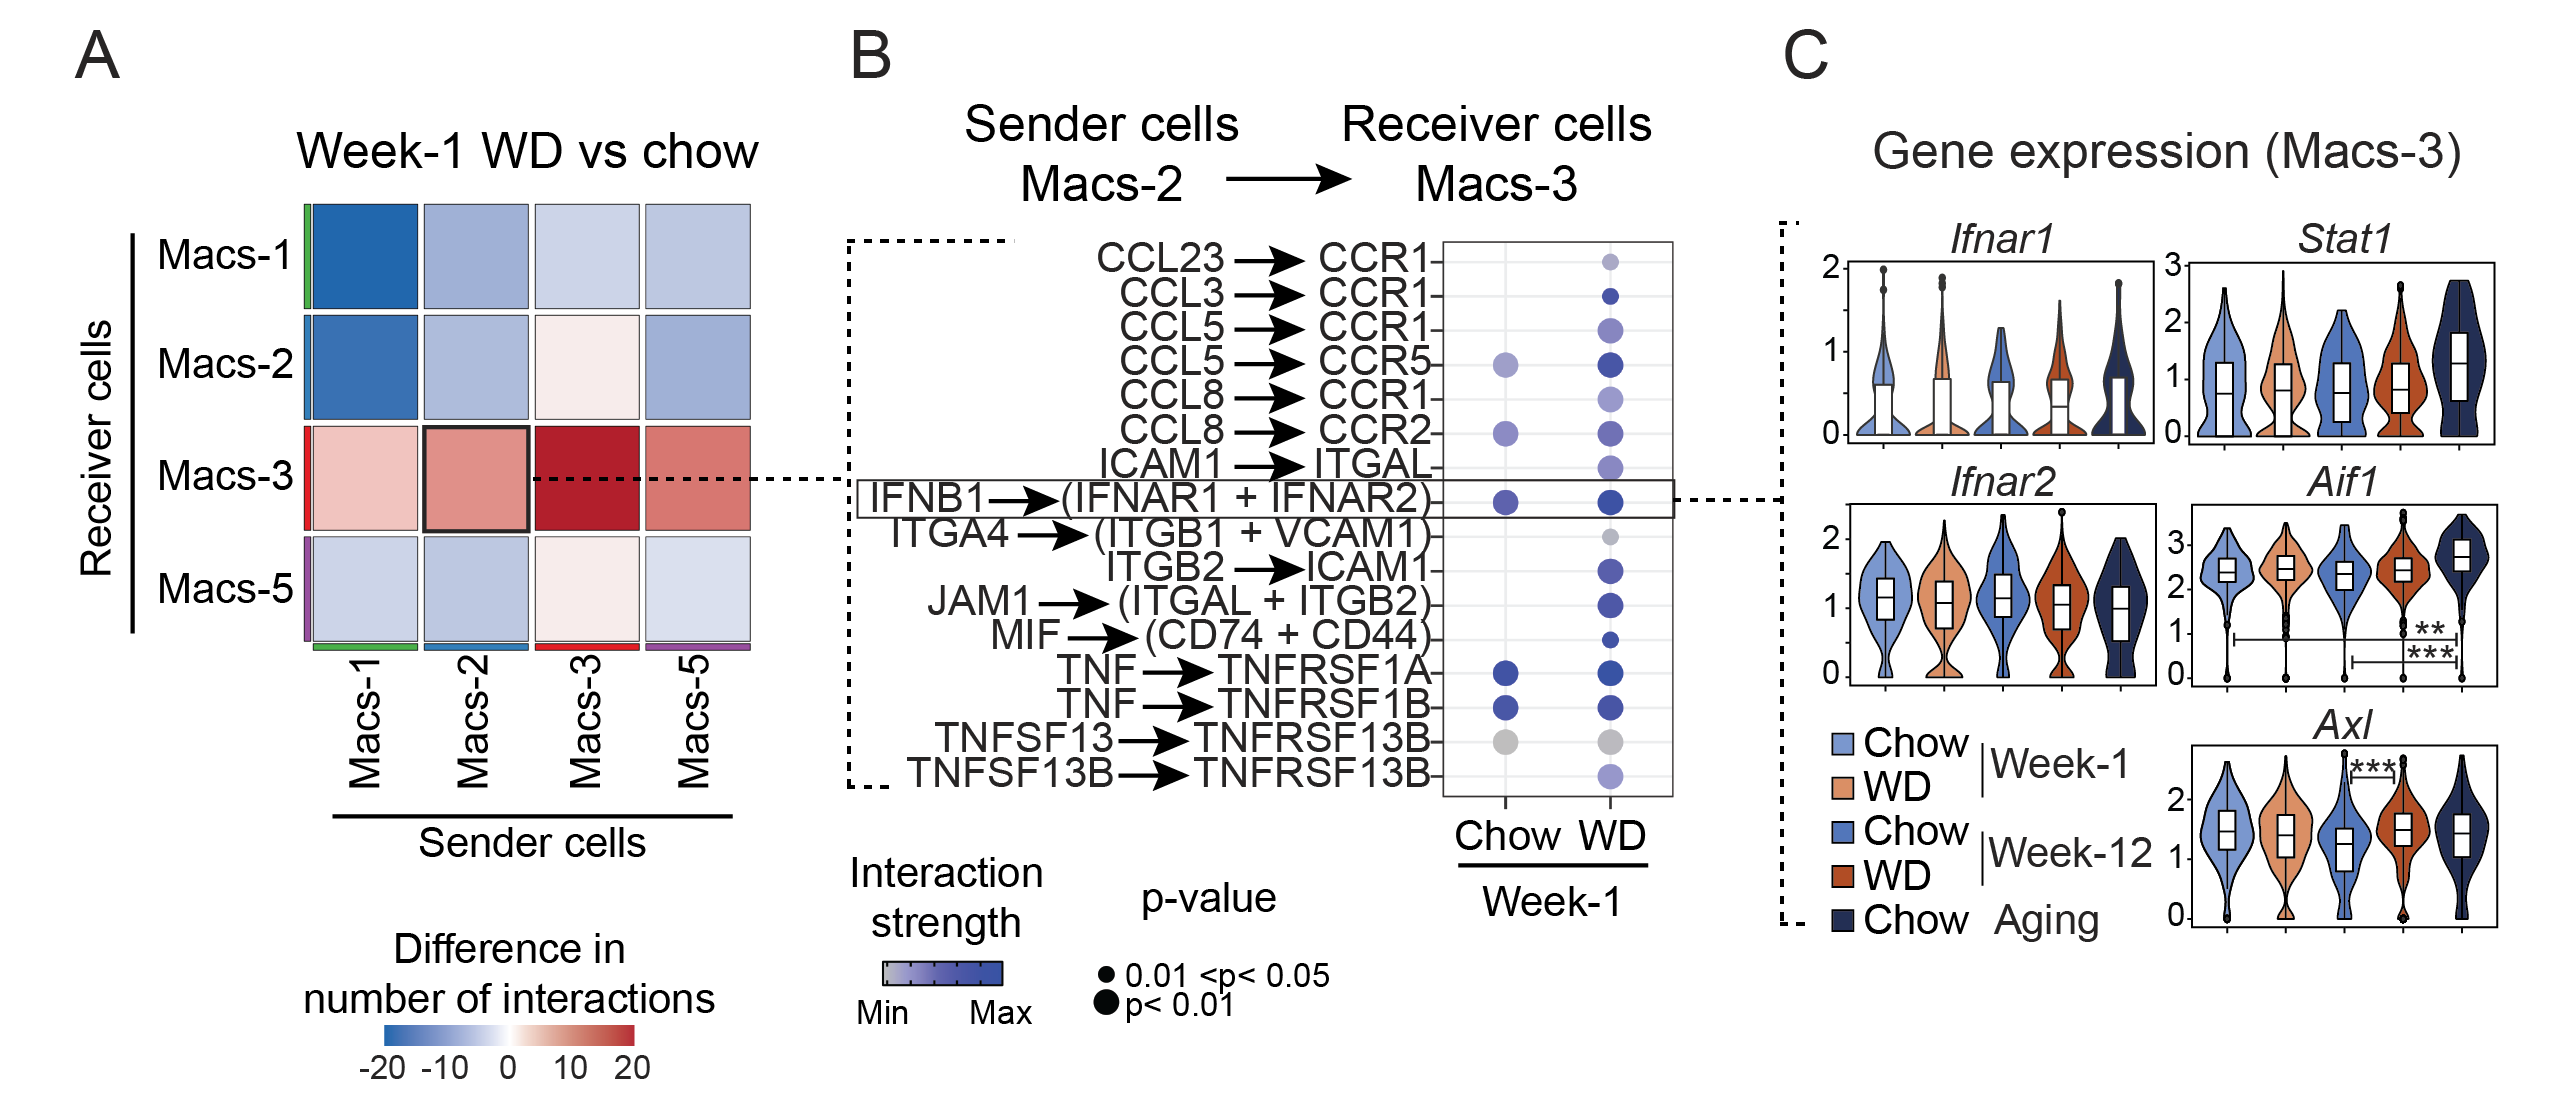
\includegraphics[width=\linewidth]{Chapter4/Fig/F2-6-01.png}
\caption[Intercellular interactions under acute overnutrition]{\textbf{Intercellular interactions under acute overnutrition.} \textbf{(A)} Heatmap depicting the difference in number of \gls{lr} interactions in the indicated macrophage sub-populations between the \gls{wd} cohorts compared to the chow diet cohorts after 1 week of feeding. In the color bar, the red (or blue) represents increased (or decreased) number of interactions in the \gls{wd} data compared to chow data. \textbf{(B)} Dot plots depicting the computed communication probability for the indicated \gls{lr} pairs, with signals from Macs-2 to Macs-3, under chow diet and one-week post-\gls{wd} conditions. The dot color and size represent the calculated communication probability and significance, respectively. p-values are computed from one-sided permutation test directly within CellChat. \textbf{(C)} Violin plots depicting the normalized expression of potential receptors and associated signaling pathway genes, originating from specified \gls{lr} pairs in Macs-3, across various experimental conditions.}
\label{fig:chp2_scrna_cellchat1}
\end{figure}

To investigate the effects of an acute \gls{wd} feeding regimen on the intercellular interactions between the sub-populations from the islet-intrinsic macrophages \textbf{(\autoref{sec:chp2_sc_macs})} in the single-cell data, we performed differential interaction analysis between \gls{wd} and normal chow diet feeding after one week (W1), using CellChat \textbf{\cite{jin_cellchat_2023}}. We excluded the proliferative Macs-4 from \gls{lri} analysis. We observed an increased number of incoming signals into the inflammatory Macs-3 \textbf{(\autoref{fig:chp2_scrna_cellchat1} A)} as well as an increase in the incoming interaction strength \textbf{(\autoref{fig:app_scrna_cellchat1}} left\textbf{)}, whereas the Macs-1 and the Macs-2 sub-populations had reduced number of incoming signals \textbf{(\autoref{fig:chp2_scrna_cellchat1} A)} as well as reduced incoming interaction strength \textbf{(\autoref{fig:app_scrna_cellchat1}} left\textbf{)}. We were particularly interested in the intercellular communications between the two inflammatory macrophage sub-populations within the islet niche, under acute \gls{wd} feeding. Therefore, we examined the up- and down-regulated \gls{lr} signaling pairs from Macs-2 to Macs-3 in the \gls{wd} compared to normal chow diet. Several interaction pairs such as cytokine:cytokine-receptors, \gls{ifn}:\gls{ifn}-receptors and \gls{tnf}:\gls{tnf}-receptors were enriched in response to \gls{wd} feeding between Macs-2 and Macs-3 \textbf{(\autoref{fig:chp2_scrna_cellchat1} B)}. Among these, notably, there was a significant enhancement in the signaling from the \textit{Ifnb1} expressing Macs-2 to the type-1 \gls{ifn} responsive Macs-3 macrophage sub-population, one week following the initiation of a \gls{wd}. This communication is characterized by the action of \gls{ifn}B1 on \gls{ifn}A receptors \textbf{(\autoref{fig:chp2_scrna_cellchat1} B)}, which explains the heightened type-1 \gls{ifn} response observed in Macs-3 \textbf{(\autoref{fig:chp2_scrna_macrophages_macs3_dge} A)}. Moreover, an increase in the expression levels of type-1 \gls{ifn} receptors and their downstream target genes (\textit{Stat1}) was detected in Macs-3 during acute \gls{wd} feeding \textbf{(\autoref{fig:chp2_scrna_cellchat1} C)}.\\

\par In summary, the interplay between the two distinct inflammatory macrophage sub-populations within the islets might possibly contribute to the \gls{wd}-induced activation of the type-1 \gls{ifn} response in Macs-3. 

\subsubsection{\large Intercellular interactions under chronic overnutrition}

The prolonged exposure to \gls{wd} feeding necessitates an investigation into its chronic effects on intercellular interactions within the islet niche. The sustained overstimulation from a \gls{wd} is likely to modify the interaction landscape between islet macrophages and T-cells, possibly leading to a persistent inflammatory state. Indeed, local T-cells have been shown to play an important role in driving inflammatory processes and insulin resistance by inducing proinflammatory cytokines and chemokines in metabolically active organs, such as the adipose tissue, liver and muscle \textbf{\cite{mclaughlin_t-cell_2014,wu_skeletal_nodate,park_role_2022}}. This promotes recruitment and phenotypic changes of macrophages. Whether such a cellular crosstalk between macrophages and T-cells occurs in the pancreas, irrespective of within or around the islets, is unclear.\\

\par We therefore investigated the chronic effects of \gls{wd} feeding on the intercellular communications within the islets by performing a differential \gls{lri} analysis between \gls{wd}


\begin{figure}[t]
\centering
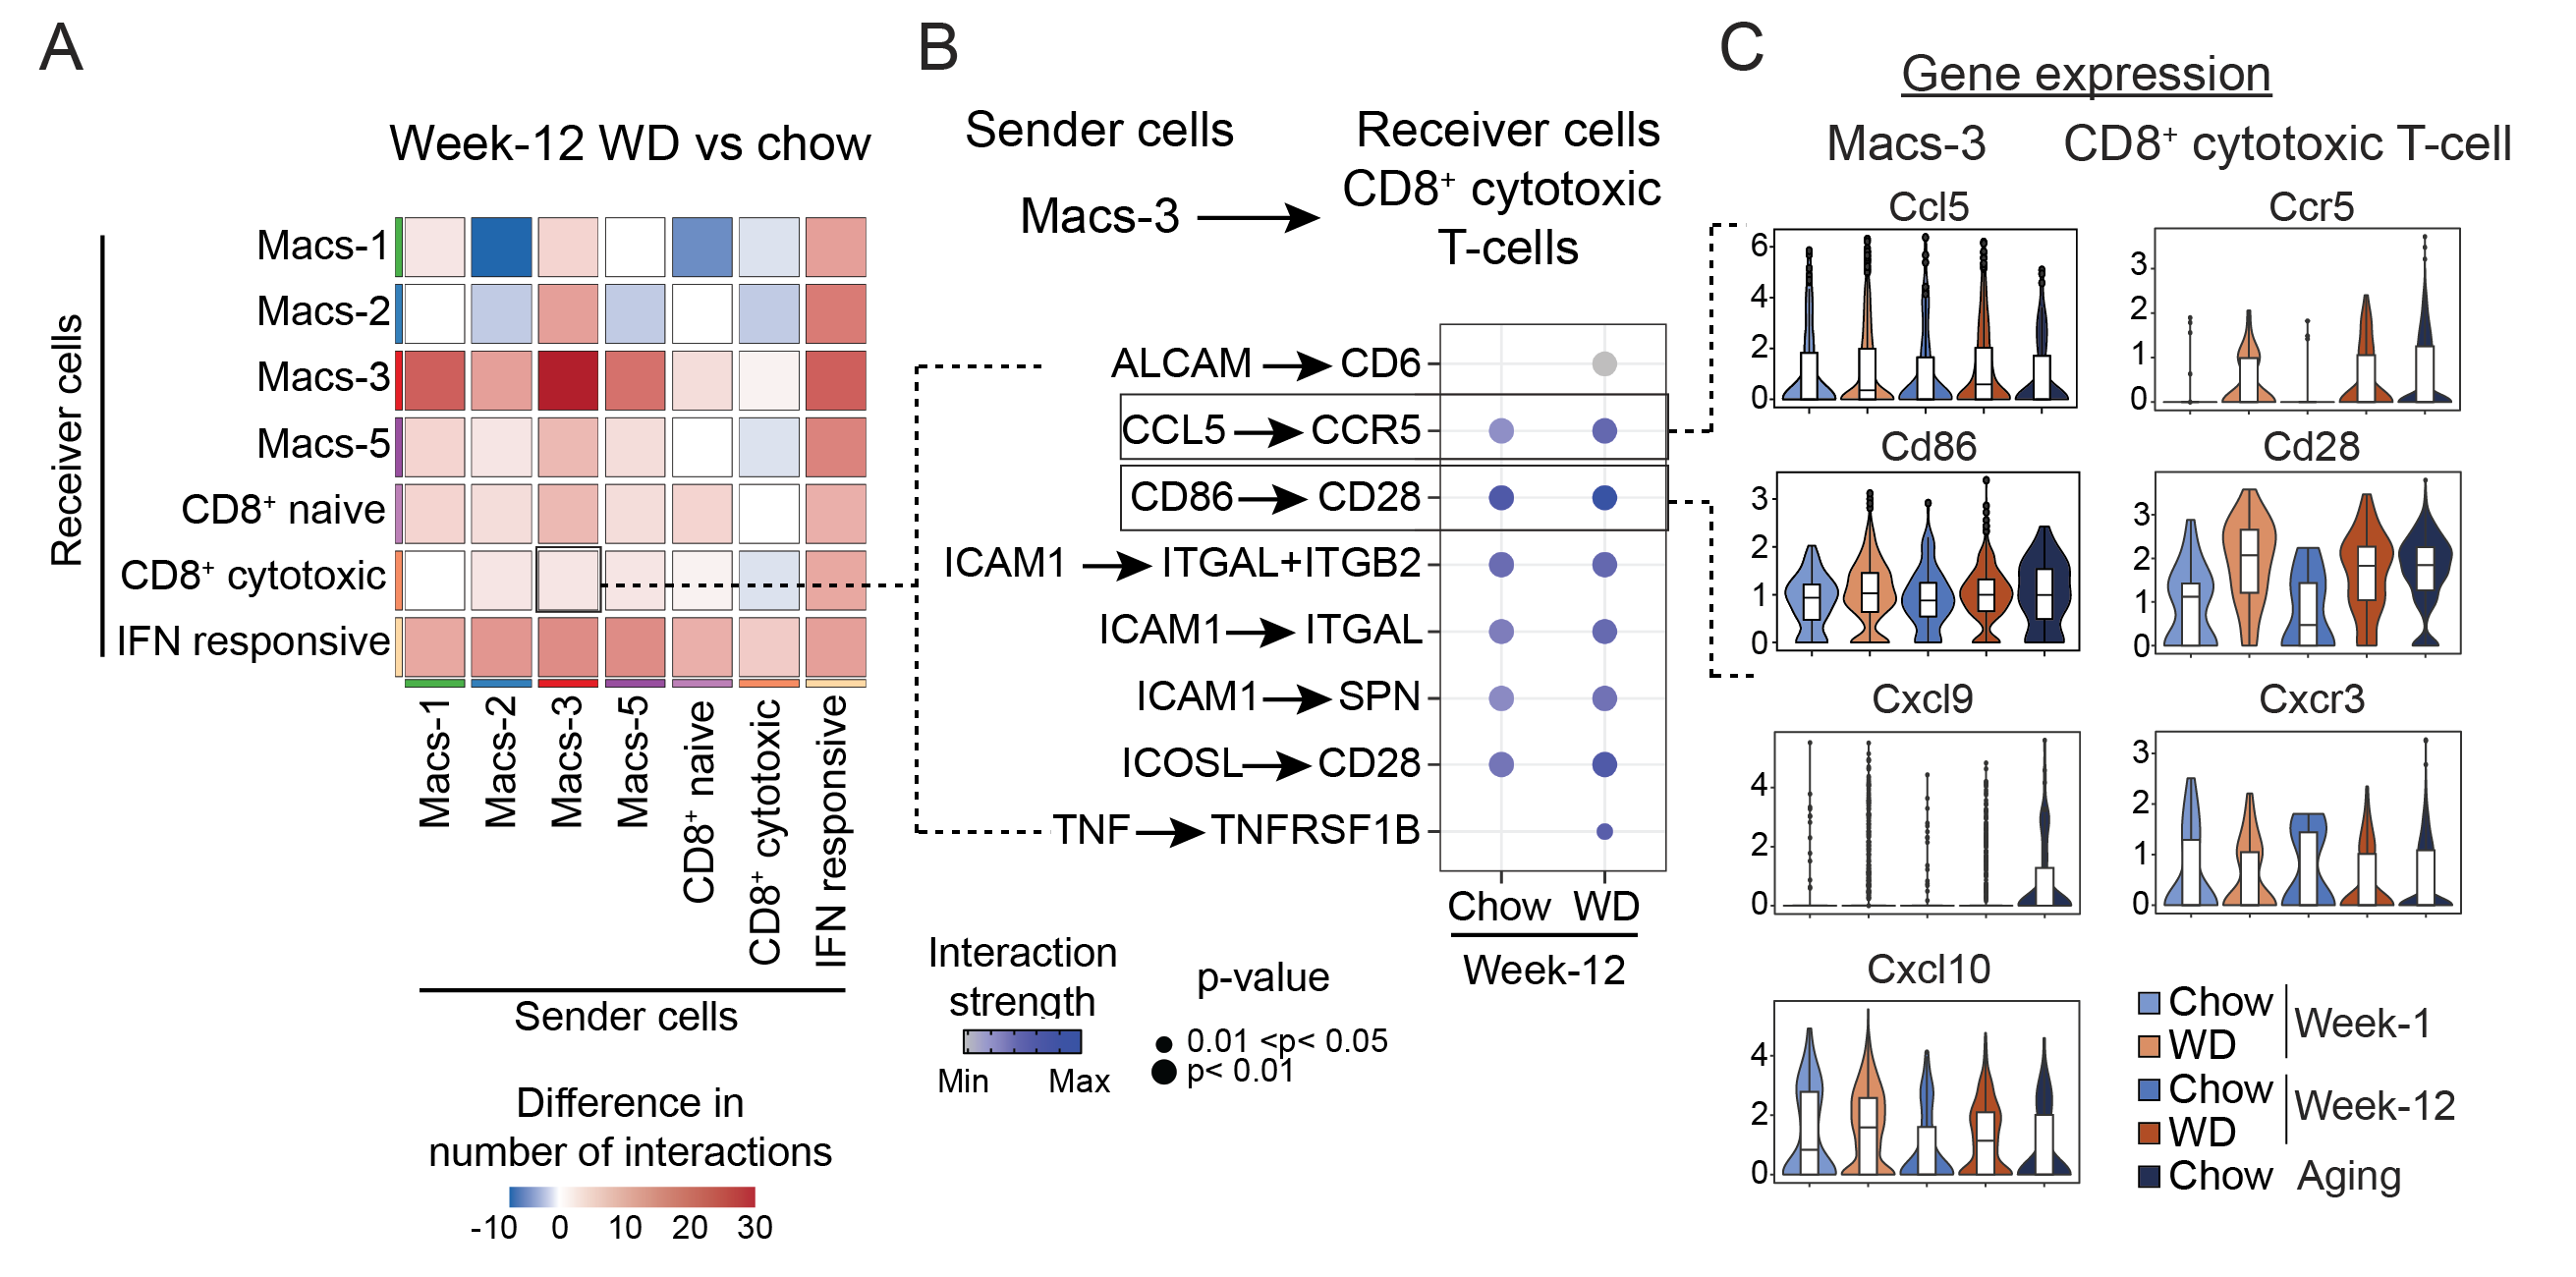
\includegraphics[width=\linewidth]{Chapter4/Fig/F2-7-01.png}
\caption[Intercellular interactions under chronic overnutrition]{\textbf{Intercellular interactions under chronic overnutrition.} \textbf{(A)} Heatmap depicting the difference in number of \gls{lr} interactions in the indicated macrophage and T-cell sub-populations between the \gls{wd} cohorts compared to the chow diet cohorts after 12 weeks of feeding. In the color bar, the red (or blue) represents increased (or decreased) number of interactions in the \gls{wd} data compared to chow data. \textbf{(B)} Dot plots depicting the computed communication probability for the indicated \gls{lr} pairs, with signals from Macs-3 to CD8\textsuperscript{+} cytotoxic T-cells, under chow diet and twelve-weeks post-\gls{wd} conditions. The dot color and size represent the calculated communication probability and significance, respectively. p-values are computed from one-sided permutation test directly within CellChat. \textbf{(C)} Violin plots depicting the normalized expression of specific ligands in Macs-3 and receptors from CD8\textsuperscript{+} cytotoxic T-cells in \textbf{(B)} across various experimental conditions.}
\label{fig:chp2_scrna_cellchat2}
\end{figure}

and normal chow diet feeding after twelve weeks (W12), using CellChat \textbf{\cite{jin_cellchat_2023}}. Similar to the W1 analysis, we included all non-proliferating macrophage sub-populations and T-cells from the single-cell data. Compared to W1 feeding, the type-1 \gls{ifn}-responsive Macs-3 depicted an overall increase in numbers of outgoing and incoming interaction signals \textbf{(\autoref{fig:chp2_scrna_cellchat2} A)} as well an increase in their corresponding interaction strengths \textbf{(\autoref{fig:app_scrna_cellchat1}} middle\textbf{)}. To further explore the crosstalk between macrophages and T-cells, we focused on the intercellular interactions between Macs-3 and CD8\textsuperscript{+} cytotoxic T-cells. With the progression of overnutrition, the activated Macs-3 sub-population increased its communication with CD8\textsuperscript{+} cytotoxic T-cells, as evidenced by increased number of interactions \textbf{(\autoref{fig:chp2_scrna_cellchat2} A)}. Notable interactions between these two sub-populations comprise the action of C-C motif chemokine ligand 5 (CCL5) secreted by Macs-3 on the C-C chemokine receptor type 5 (CCR5) receptor present on CD8\textsuperscript{+} cytotoxic T-cells, as well as the engagement of the co-stimulatory signaling molecules cluster of differentiation 86 (CD86) on Macs-3 with cluster of differentiation 28 (CD28) on CD8\textsuperscript{+} cytotoxic T-cells, which are required for T-cell activation and survival \textbf{(\autoref{fig:chp2_scrna_cellchat2} B)}. Within the Macs-3 sub-population, the expression of \textit{Ccl5} was exclusively triggered by \gls{wd} feeding, while \textit{Cd86} expression was common to both overnutrition and aging \textbf{(\autoref{fig:chp2_scrna_cellchat2} C)}. Additionally, the communication between Macs-3 and CD8\textsuperscript{+} cytotoxic T-cells featured a \gls{wd}-specific involvement of \textit{Cxcl10}, which acts through the \textit{Cxcr3} receptor on the CD8\textsuperscript{+} cytotoxic T-cells. Conversely, under aging conditions, \textit{Cxcl9} is the preferentially expressed ligand for \textit{Cxcr3} \textbf{(\autoref{fig:chp2_scrna_cellchat2} C)}.\\

\par It is well-established that \textit{Cxcl9} expression is triggered by the canonical type-1 \gls{ifn} pathway, whereas \textit{Ccl5} and \textit{Cxcl10} transcription is induced by the non-canonical type-1 \gls{ifn} signaling pathway \textbf{\cite{mazewski_type_2020}}, reflecting the distinct activation states of Macs-3 under the two different stress conditions \textbf{(\autoref{fig:chp2_scrna_macrophages_macs3_dge})}. Furthermore, the Macs-2 sub-population, which also exhibited non-canonical type-1 \gls{ifn} responses during overnutrition, up-regulated the transcription of \textit{Ccl5} and \textit{Cxcl10} in response to \gls{wd} compared to chow diet feeding and aging \textbf{(\autoref{fig:app_scrna_macrophages_macs2_dge})}. This suggests that Macs-2 cells may also contribute to the overnutrition- and aging- specific communication between macrophages and T-cells. Importantly, our \gls{imc} analysis revealed that F4/80\textsuperscript{-} and F4/80\textsuperscript{\textit{low}} macrophages, corresponding to the Macs-2 and Macs-3 sub-populations in the \gls{scr} data, respectively, show a positive correlation with CD8\textsuperscript{+} activated effector-like T-cells in the pancreatic tissue therefore indicating a mutual dependency between these sub-populations \textbf{(\autoref{fig:chp2_imc_correlation} A)}. Additionally, CD8\textsuperscript{+} and CD11c\textsuperscript{+} cells were frequently observed, both in the exocrine pancreas and within pancreatic islets and in close proximity to each other \textbf{(\autoref{fig:chp2_imc_correlation} B)}. This further suggests the possibility of intercellular \gls{lri}s thereby perpetuating local islet inflammation.\\

% This suggests that the cytokine / chemokine-mediated communication between Macs-2 / Macs-3 sub-populations and the T-cells significantly differs between overnutrition and aging conditions, even though CD86 and CD28 mediated interactions remain consistent across these scenarios (\textbf{Fig.\ref{suppl_fig:cell_cell2}}).


\begin{figure}[t!]
\centering
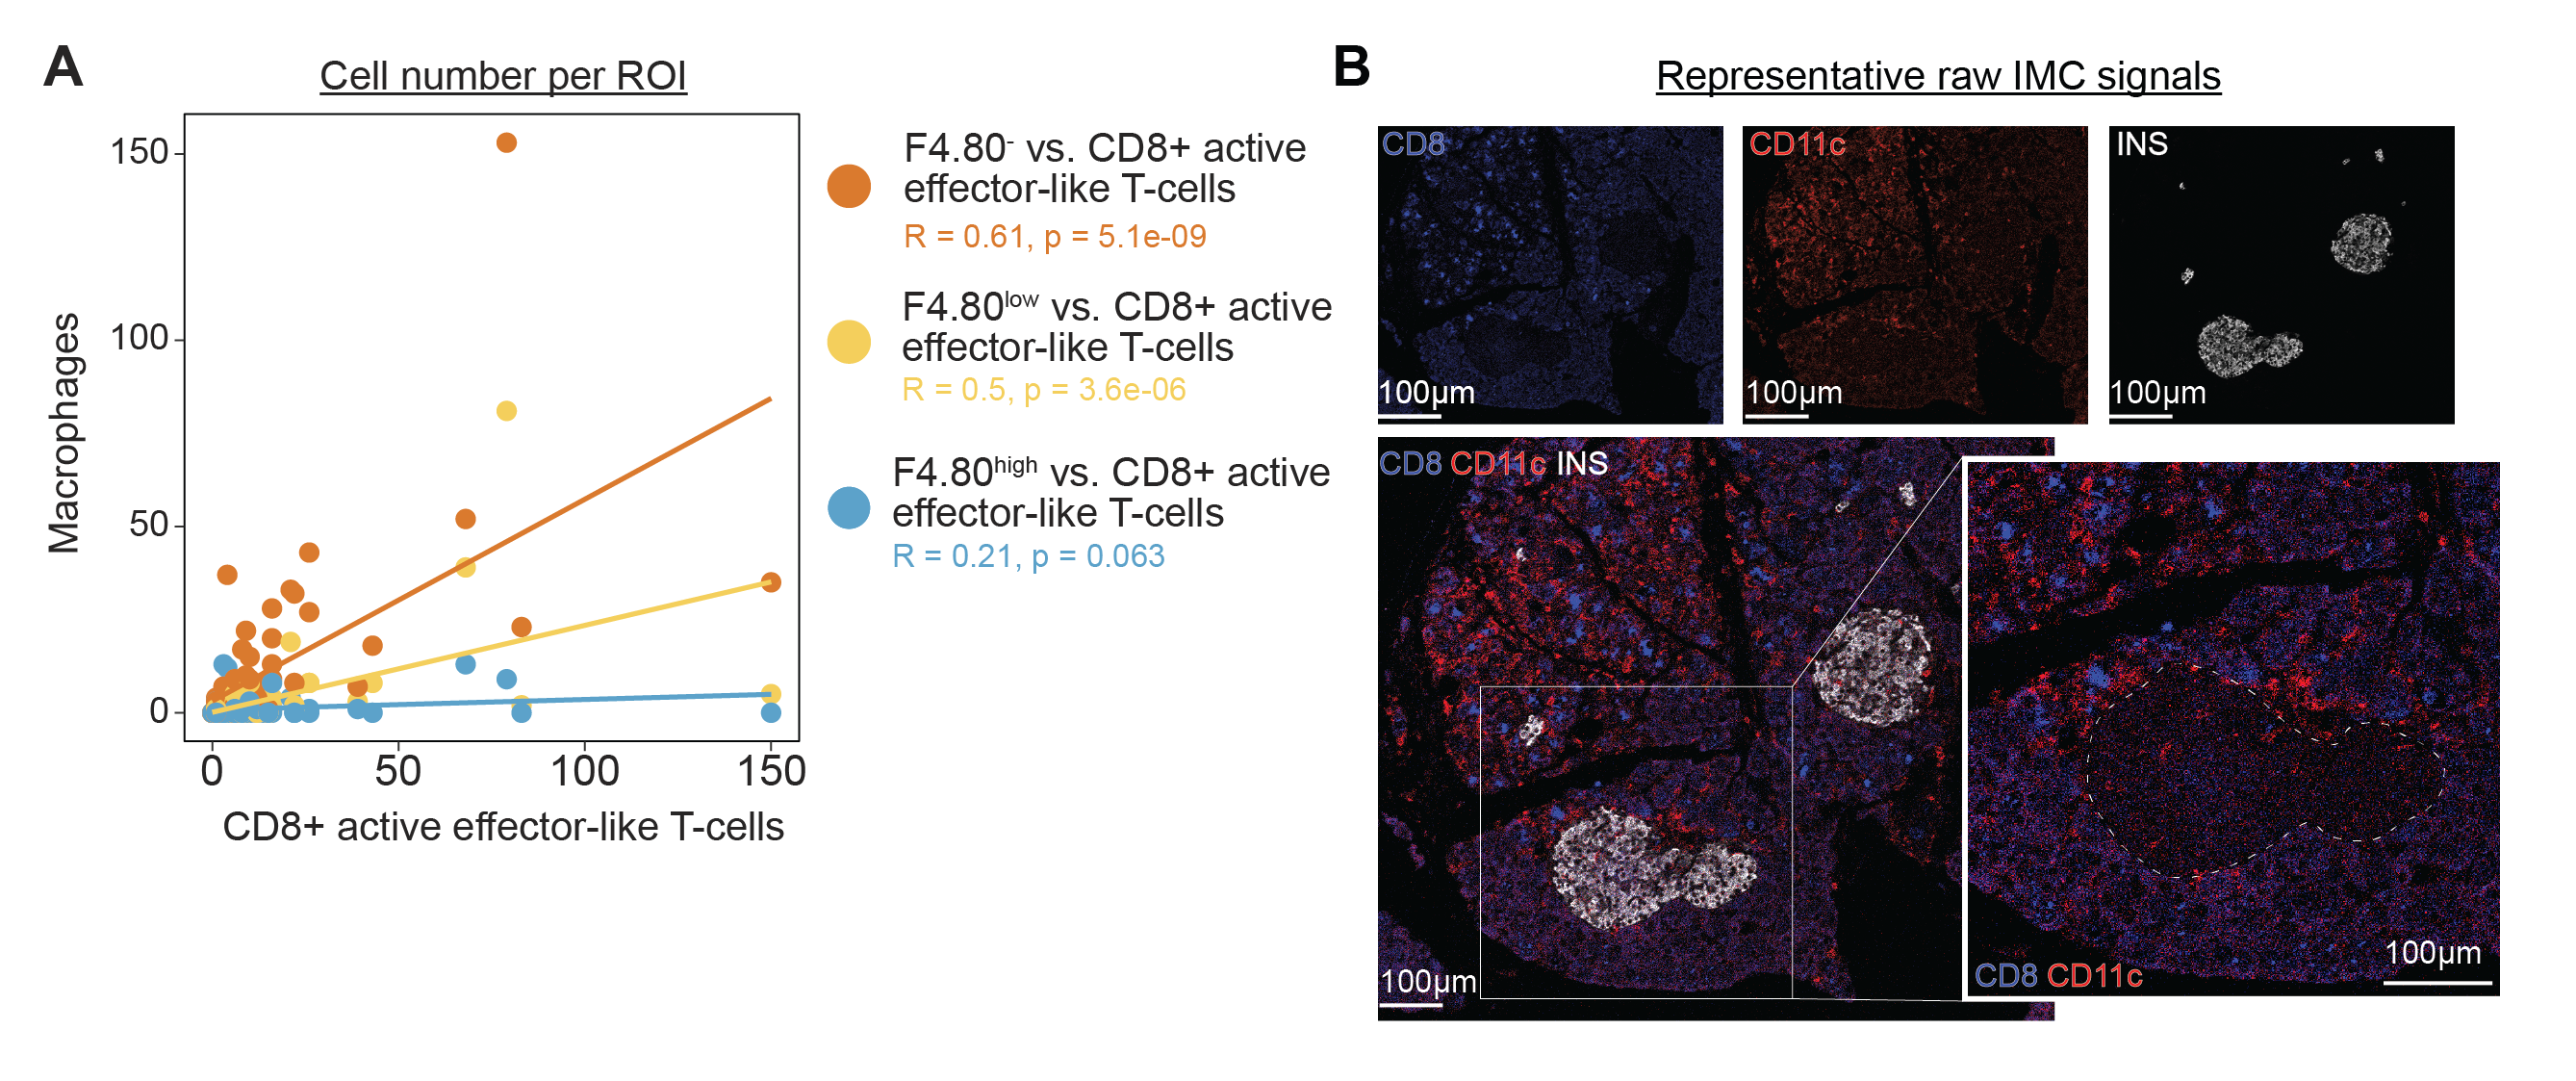
\includegraphics[width=\linewidth]{Chapter4/Fig/F2-8-01.png}
\caption[Co-localization of macrophages and T-cells within pancreas]{\textbf{Co-localization of Macrophages and T-cells within pancreas and pancreatic islets.} \textbf{(A)} Scatter plot depicting the pearson correlation between the counts of CD8\textsuperscript{+} activated effector-like T-cells and three macrophage sub-populations from the \gls{imc} analysis, within the same \glspl{roi}. Solid lines represent best fit in each correlation analysis. Pearson correlation coefficients and p-values for the corresponding macrophage sub-populations are included. \textbf{(B)} Representative \gls{roi} showing raw signals from the CD8 (blue), CD11c (red), and INS (white) channels. Scale bar, 100 \textmu m. \textit{This data and figure were originally generated by Dr. Matthias Barone and reused here with permission.}}
\label{fig:chp2_imc_correlation}

\end{figure}


\subsubsection{\large Intercellular interactions during aging}

%Observations from our data and evidence from a previous study points to the accumulation of T-cells in non-diabetic islets during aging \textbf{\cite{denroche_t_2021}}. Furthermore, another study indicated that 

\par  We therefore examined intercellular interactions during aging compared to chow diet-fed non-aging cohorts for the non-proliferating macrophage and CD8\textsuperscript{+} T-cell sub-populations. Similar to the observations of increased interaction strengths of the sub-populations in response to \gls{wd}, aging also resulted in similar increases in strengths of the incoming and outgoing interactions for the four macrophage sub-populations as well as the CD8\textsuperscript{+} naive and cytotoxic T-cells \textbf{(\autoref{fig:app_scrna_cellchat1}} right\textbf{)}. We observed that the CD8\textsuperscript{+} memory T-cells depicted the strongest interactions as well as a higher number of outgoing and incoming interactions amongst all the other sub-populations during aging \textbf{(\autoref{fig:chp2_scrna_cellchat3} A; \autoref{fig:app_scrna_cellchat1}} right\textbf{)}. This could be attributed to the aging-specific abundance of the CD8\textsuperscript{+} memory T-cells \textbf{(\autoref{fig:chp2_scrna_tcells1} B; \autoref{tab:app_scrna_cellnumbers})}. Similarly, despite the increase in number of interactions involving the \gls{ifn}-responsive T-cells during both, chronic \gls{wd} feeding and aging, we could not infer any significant signaling interactions using CellChat, possibly due to the overall low number of \gls{ifn}-responsive T-cells in the adult cohorts \textbf{(\autoref{fig:chp2_scrna_tcells1} B; \autoref{tab:app_scrna_cellnumbers})}. Interestingly, we observed more interactions in the aging cohort compared to adult cohorts of 10-week-old and 21-week-old mice in all sub-populations \textbf{(\autoref{fig:chp2_scrna_cellchat3} A)} indicating an altered landscape of immune crosstalk during aging.

\begin{figure}[b!]
\centering
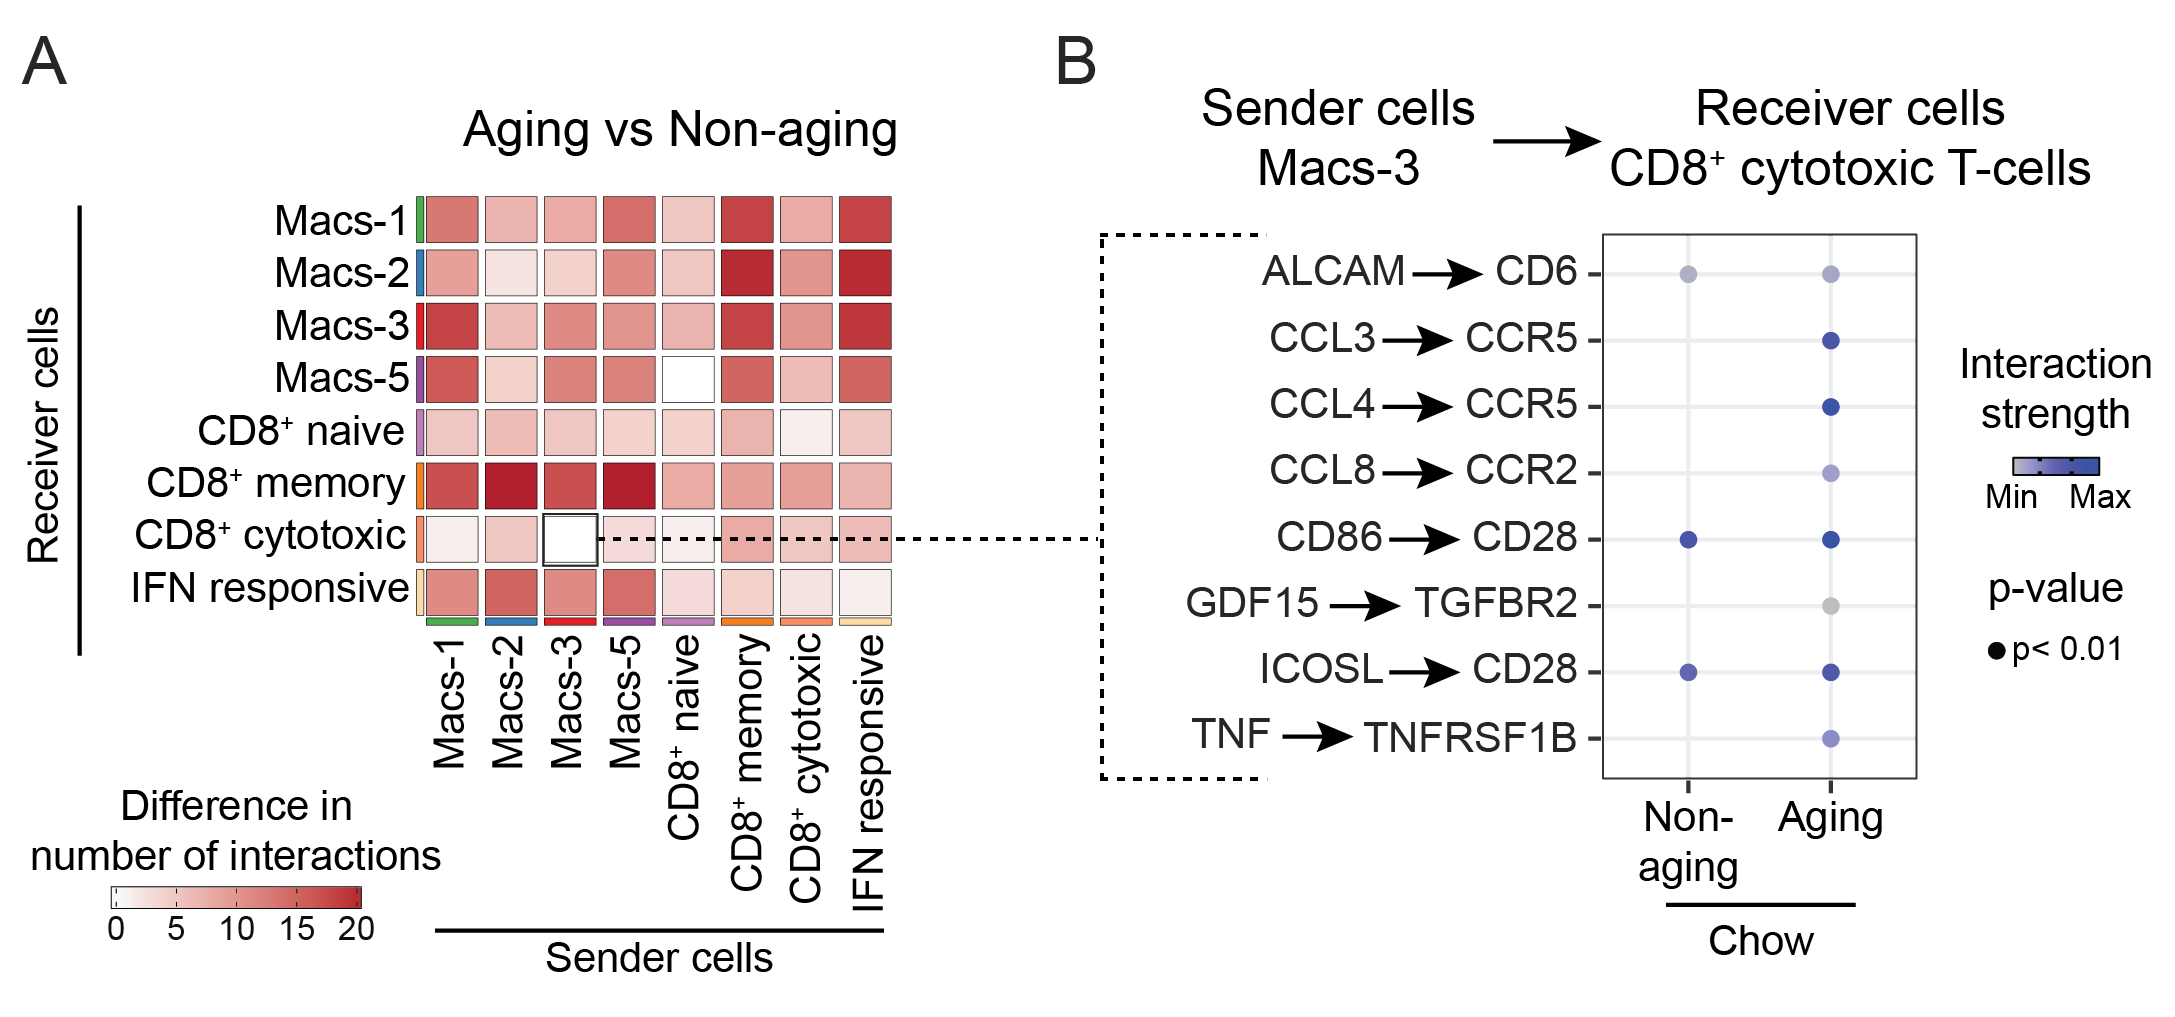
\includegraphics[width=\linewidth]{Chapter4/Fig/F2-A1-v3-02.png}
\caption[Intercellular interactions under aging]{\textbf{Intercellular interactions under aging.}
\textbf{(A)} Heatmap depicting the difference in number of \gls{lr} interactions in the indicated macrophage and T-cell sub-populations between the aging cohorts compared to the non-aging cohorts. In the color bar, the red represents the increased number of interactions in the aging data compared to non-aging data. \textbf{(B)} Dot plot depicting the computed communication probability for the indicated \gls{lr} pairs, with signals from Macs-3 to CD8\textsuperscript{+}  cytotoxic T-cells, under aging and non-aging conditions. The dot color and size represent the calculated communication probability and significance, respectively. p-values are computed from one-sided permutation test directly within CellChat.}
\label{fig:chp2_scrna_cellchat3}
\end{figure}

\par To examine the overlap of intercellular interactions between macrophages and T-cells during overnutrition and aging, we focused on interactions between Macs-3 and CD8\textsuperscript{+} cytotoxic T-cells. In line with the observations of \gls{wd}-specific expression of \textit{Ccl5} \textbf{(\autoref{fig:chp2_scrna_cellchat2} C)}, interactions that were found to be enriched between Macs-3 and CD8\textsuperscript{+} cytotoxic T-cells during aging did not include CCL5. Instead, Macs-3 secreted other chemokines such as CCL3 and CCL4 which utilized the CCR5 receptor, and CCL8 which interacted with the CCR2 receptor on the cytotoxic T-cells \textbf{(\autoref{fig:chp2_scrna_cellchat3} B)}. Despite this contrast in interactions in response to \gls{wd} feeding and aging, the CD86-CD28 co-stimulatory interaction was shared between the two stresses \textbf{(\autoref{fig:chp2_scrna_cellchat3} B)}.\\

\par Collectively, our multi-modal analysis suggests that both of the inflammatory macrophage sub-populations in the pancreas and pancreatic islets actively communicate with cytotoxic T-cells. This communication relies on distinct chemokine / cytokine profiles under \gls{wd} and aging conditions, but utilizes the same co-stimulatory mechanisms. 

%\clearpage

\section[Summary]{Summary}
\label{sec:chp2_summary}

\par Characterizing the phenotypes of immune cells in the pancreas and pancreatic islet during overnutrition and aging presents a significant challenge. In this study, we employed \gls{imc} and \gls{scr} to profile immune cells within pancreatic tissue and pancreatic islets. Our goal was to integrate their phenotypic characteristics with spatial localization, providing a more comprehensive understanding of their roles under these conditions.\\

\par We discovered that obesity, induced by \acrfull{wd} feeding, significantly accelerated the age-dependent accumulation of multiple immune cell populations within the pancreas and around the pancreatic islets. These populations included CD8\textsuperscript{+} cytotoxic T-cells and F4/80\textsuperscript{\textit{low}} (Macs-3) macrophages. This likely points to the stronger impact of diet on the dynamics of certain immune cells. These sub-populations also depicted altered molecular profiles and detailed intercellular interaction analyses between these sub-populations revealed that the inflammation accelerated by the \gls{wd} diverged from typical age-related patterns, exhibiting a unique type of type-1 \gls{ifn} response. Our multi-modal approach also provided a detailed spatio-temporal characterization of other immune cells, islet endocrine cells as well as other relevant cell populations during overnutrition and aging.\\

\par These findings are crucial for understanding the progression and development of \gls{t2d} and underscores the importance of considering both dietary and age-related factors in diabetes research and their roles in modulating inflammation that affects disease progression.\\

\newpage\null\thispagestyle{empty}


% By combining single cell expression profiling and common genetic variation of over one hundred individuals we can begin to assess the impact of genetic variability on expression in a continuous manner across early human development.
% We have imputed genotypes for all of our 125 samples \cite{kilpinen2017common}, so this study allows discovery of single cell eQTL along differentiation. 
% Using the developmental stages just described and methods similar to those described in the previous chapter, we mapped eQTL in each of the \gls{ipsc}, mesendo and defendo populations, yielding 1,833, 1,702 and 1,342 eGenes, respectively. 
% Briefly, we quantified each gene’s average expression level for each donor, experiment, and differentiation stage\footnote{This approach is the same as what is described in the first part of \textbf{Chapter \ref{chapter3}}, and similar to the `dr-mean' described in \textbf{section \ref{sec:best_practice}}, except that the aggregation is done at the experiment level rather than the sequencing run level.}, before using a linear mixed model to test for \textit{cis} eQTL, adapting approaches used for bulk RNA-seq profiles (+ and - 250 kb, MAF >5\% \cite{kilpinen2017common}).\\

% For comparison, we also performed eQTL mapping in cells collected on day1 and day3, i.e. the experimental time points commonly used to identify cells at mesendo and defendo stages \cite{hannan2013production}.
% Interestingly, this approach identified markedly fewer eGenes: 1,181 eGenes at day1, and 631 eGenes at day3.
% These results demonstrate the power of using the single-cell RNA-seq profiles to define relatively homogeneous differentiation stages in a data-driven manner (\textbf{Fig. \ref{fig:endodiff_stage_eqtl}}). 
% Notably, this observation was not merely a consequence of differences in the number of cells or donors considered in each cell population (\textbf{Fig. \ref{fig:endodiff_stage_eqtl}}). \\

% \begin{figure}[h]
% \centering
% \includegraphics[width=14cm]{Chapter4/Fig/endodiff_eqtl.png}
% \caption[eQTL maps of iPSC, mesendo, defendo]{\textbf{Mapping single cell eQTL at different developmental stages.}\\
% (a) Illustration of the single cell eQTL mapping strategy at various stages of differentiation.
% Shown is an example of a defendo-specific eQTL. 
% Box plots of gene expression stratified by the allelic state of
% rs9648854 at each stage, showing an association between rs9648854 and \textit{CNTNAP2} expression at the defendo stage, but not at earlier stages. 
% (b) Comparison of eQTL mapping using different strata of all cells.
% The use of pseudotime-based stages increases the number of detectable eQTL, compared to using the corresponding time point of collection.
% Bar plots represent number of eGenes (genes with at least one eQTL, at FDR < 10\%).
% (c) Similar to b, the number of donors for which gene expression data were assayed at day0, day1, and day3, compared to the number of donors in the pseudotime-inferred mesendo and defendo stages.
% (d) As for (c), with the number of cells.
% \url{https://github.com/ebiwd/EBI-Icon-fonts} by EBI Web Development is licensed under CC BY 4.0. }
% \label{fig:endodiff_stage_eqtl}
% \end{figure}

% Profiling multiple stages of endoderm differentiation allowed us to assess at which stage along this process individual eQTL can be detected as well as the level of sharing of genetic signal across time. 
% We observed substantial regulatory and transcriptional remodelling upon endoderm differentiation of iPSCs, with over 30\% of eQTL being specific to a single stage.
% To define pairwise replication (and conversely specificity) between two sets of test results we considered nominal significance (p value < 0.05) and consistent direction of the effect size.
% Importantly, we observed that stage-specificity of eQTL was not significantly explained by stage-specific gene expression (\textbf{Fig. \ref{fig:endodiff_stage_specific_eqtl}}).
% Our differentiation time course covers developmental stages that have never before been accessible to genetic analyses of molecular traits and thus this study provides the first eQTL maps at mesendoderm and definitive endoderm.
% We next explored whether any of the eQTL identified in these two studies were novel, and found that 349 of them have not been reported in either a recent iPSC eQTL study based on bulk RNA-seq \cite{mirauta2018population}, or in a compendium of eQTL identified from 49 tissues as part of the GTEx project \cite{gtex2017genetic}.
% An eQTL was defined as novel when it was not reported as lead variant (FDR < 10\%) in any of the tissues considered nor was it in \gls{ld} (see \textbf{section \ref{sec:gwas}}) with any reported lead variant, \gls{ld} assessed using $r^2<0.2$.\\

% Finally, we investigated the presence of lead switching events.
% These correspond to two distinct genetic variants that are identified as lead eQTL for the same gene at different stages of differentiation (at LD: $r^2<0.2$),
% We found lead switching events for 155 eGenes (an example in iPSC and defendo is illustrated in \textbf{Fig. \ref{fig:endodiff_stage_specific_eqtl}}). 
% To explore the potential regulatory role of these variants, we investigated whether the corresponding genetic loci also featured changes in histone modifications during differentiation. 
% To do so, we used ChIP-Sequencing to profile five histone modifications that are associated with promoter and enhancer usage (H3K27ac, H3K4me1, H3K4me3, H3K27me3, and H3K36me3) in human embryonic stem cells (hESCs) that were differentiated towards endoderm (using the same protocol employed above) and measured at equivalent time points (i.e. day0, day1, day2, day3, see \textbf{section \ref{sec:endodiff_chipseq}} for detailed experimental methods). 
% Interestingly, we observed corresponding changes in the epigenetic landscape for 20 of the lead switching events (i.e. stage-specific lead variants overlapped with stage-specific changes in histone modification status), suggesting a direct mechanism (\textbf{Fig. \ref{fig:endodiff_stage_specific_eqtl}}).

% \begin{figure}[htbp]
% \centering
% \includegraphics[width=12cm]{Chapter4/Fig/endodiff_stage_specific.png}
% \caption[Stage-specific eQTL]{\textbf{Stage-specific eQTL.}\\
% (a) Proportion of eQTL that are specific to a single stage, shared across two
% stages, or observed across all stages (sharing defined as a lead eQTL variant at one stage with nominal p value < 0.05 and consistent direction
% at another stage).
% (b) Proportion of stage-specific eGenes (genes with a stage-specific eQTL) that are expressed only at a single stage, expressed at two stages, or expressed at all stages. 
% Expressed is defined as normalised log2(CPM+1) > 2. 
% CPM: counts per million.
% (c) A lead switching event consistent with epigenetic remodelling. 
% The overlap of H3K4me1 with the eQTL SNPs across differentiation time points is shown by the coloured bars.}
% \label{fig:endodiff_stage_specific_eqtl}
% \end{figure}
% The availability of large numbers of cells per donor across a continuous differentiation trajectory from pluripotent stage to definitive endoderm enabled the analysis of dynamic changes of eQTL strength at fine-grained resolution. 
% To formally test for eQTL effects that change dynamically across differentiation (dynamic eQTL), we tested for associations between pseudotime (both linear and quadratic) and the genetic effect size using allele-specific expression (ASE) and a linear model (see \textbf{Box \ref{box:ase}}):

% \begin{equation}\label{eq:endodiff_ase_pseudotime}
%     \mathrm{ASE} = \alpha_1 \mathrm{pseudotime} + \alpha_2 \mathrm{pseudotime}^2 + \boldsymbol{\psi},
% \end{equation}

% where the genetic effect is defined based on \gls{ase} at the level of single cells, i.e. quantified as fractional read counts overlapping each allele for a given gene-SNP pair (see details in \textbf{Box \ref{box:ase}}).
% We assessed significance using a likelihood ratio test with two degrees of freedoom (i.e. $H_0: \alpha_1 = \alpha_2 = 0$). 
% For this analysis, we focused on the joint set of 4,422 eQTL lead variants (4,470 SNP-gene pairs) discovered at the iPSC, mesendo, and defendo stages and explored how they were modulated by developmental time (using our inferred pseudotime).
% In this way, we uncovered a total of 899 time dynamic eQTL at FDR < 10\%, including a substantial fraction of eQTL that were not identified as stage-specific by the discrete approach previously used (\textbf{page \pageref{fig:endodiff_stage_specific_eqtl}}).
% This analysis is somewhat complementary to the eQTL map perfomed on discrete differentiation stages (\textbf{Fig. \ref{fig:endodiff_stage_eqtl}}), which identified substantial stage-specific effects (\textbf{Fig. \ref{fig:endodiff_stage_specific_eqtl}}).
% Namely, we observe that in general stage-specific effects are weaker and unique to certain cell types.
% In contrast, the dynamic eQTL identified are detected to a certain extent across all cell types, but the strength of the effect is modulated by differentiation time. \\

% One obvious explanation for these subtle dynamic changes could be that they are simply reflecting changes in overall expression. 
% To visualise this, we used a sliding-window approach. 
% Because we need a rather large amount of cells to reliably estimate expression abundance for each individual, we slide a window containing 25\% of the cells along pseudotime by a step of 2.5\% cells.
% In each window, we considered average expression quantifications and estimate genetic effects using eQTL mapping, essentially performing the same analysis we performed in developmental stages in \textbf{section \ref{sec:endodiff_eqtl}}, now in each window.
% In parallel, we reassessed each eQTL in each window taking advantage of the full length transcript sequencing to measure \gls{ase}.
% Here, in each window, we quantified the deviation from 0.5 of the expression of the minor allele at the eQTL (ratio of reads phased to eQTL variants, \textbf{Fig. \ref{fig:endodiff_sliding_window}}). 
% Notably, ASE can be quantified in each cell and is independent of expression level, thus mitigating technical correlations between differentiation stage and genetic effect estimates (\textbf{Box \ref{box:ase}}). 

%****** Box on ASE to quantify genetic effects ******

% \newpage

% \begin{Comment}
% \hspace{-2.5mm}\textbf{Box\ref{box:ase}: Quantifying genetic effects using ASE}\label{box:ase}\\
% \small
% When full-transcript (phased) data is available, \gls{ase} can be used to quantify the genetic effect of a variant on expression as a single ratio, by quantifying the relative expression of one allele over the other.
% For a given eQTL - and the corresponding eQTL variant and eGene -  we i) select individuals that are heterozygous at the eQTL SNP of interest, ii) consider all exonic heterozygous variants on the corresponding eGene, iii) map reads to these SNPs, iv) aggregate all reads coming from the same chromosome and v) compute the ratio. 
% Conventionally, we look at ratios < 0.5 i.e. in the numerator goes the allele with fewer reads mapped to it:

% \vspace{5mm}

% \includegraphics[width=15cm]{Chapter4/Fig/ASE.png}

% If one of these alleles is more responsive to a particular environmental factor (e.g. because of preferential transcription factor binding), then \gls{ase} is expected to vary consistently with that factor. 
% This observation has previously been used to identify GxE interactions in gene expression across individuals \cite{knowles2017allele}. 
% Critically, these \gls{ase} tests are internally matched, because potentially confounding batch effects and technical variation should affect both alleles in each cell similarly.
% Additionally, this test increases power by reducing the number of parameters to estimate, i.e. instead of the standard test for interactions:  

% \begin{equation*}
%     \mathrm{expression} = \sum_{k=1}^{K} \mathbf{e}_k\alpha_k + \mathbf{g}\beta +
%     \sum_{k=1}^{K} \mathbf{g} \odot \mathbf{e}_k\gamma_k + \boldsymbol{\psi},
% \end{equation*}

% where for each of K environments $\mathbf{e}_k$ two terms must be added (to account for E and GxE), resulting in (2*K + 2) parameters needing to be estimated (including one effect size $\beta$ and the variance explained by the noise term $\sigma_n^2$, from $\boldsymbol{\psi} \sim \mathcal{N}(\mathbf{0}, \sigma_n^2\mathbf{I_n})$), we can run:

% \begin{equation*}
%     \mathrm{ASE} = \sum_{k=1}^{K} \mathbf{e}_k\alpha_k + \boldsymbol{\psi}, 
% \end{equation*}
% where we can test directly the effect of the K environments on ASE and therefore only K+1 parameters need estimation (the K $\alpha_k$'s and $\sigma_n^2$).

% \end{Comment}

% \begin{figure}[h]
% \centering
% \includegraphics[width=15.5cm]{Chapter4/Fig/endodiff_running_average.png}
% \caption[Schematic of the sliding window approach]{\textbf{Schematic of the sliding window approach.}\\
% Cells are binned based on pseudotime ordering, to (a) quantify average expression, (b) perform eQTL mapping, and (c) quantify average ASE.
% Each bin includes 25\% of cells, binned at incremental steps of 2.5\%.}
% \label{fig:endodiff_sliding_window}
% \end{figure}

% Both methods result in a measure of genetic effect dynamics, i.e. changing strength of genetic effects along differentiation. 
% Reassuringly, the two approaches were highly consistent across pseudotime (\textbf{Fig. \ref{fig:endodiff_dynamic_eqtl}}).
% To explore this hypothesis, we clustered the top dynamic eQTL (FDR <1\%) jointly based on both the relative gene expression dynamics (global expression changes along pseudotime, quantified in sliding windows as above), and on the genetic effect dynamics (using ASE). 
% This identified four basic dynamic patterns (\textbf{Fig. \ref{fig:endodiff_dynamic_eqtl}}): decreasing early (cluster A), decreasing late (cluster B), transiently increasing (cluster C), and increasing (cluster D). 
% \begin{figure}[htbp]
% \centering
% \includegraphics[width=15.5cm]{Chapter4/Fig/endodiff_pseudo_heatmap.png}
% \caption[Dynamic eQTL]{\textbf{Dynamic eQTL.}\\
% Clustered heatmap of global expression levels, eQTL effect sizes, and ASE across pseudotime for the top 311 genes with the strongest dynamic eQTL effects (FDR < 1\%; out of 785 at FDR < 10\%). 
% For each gene, the dynamic profiles of gene expression and ASE were jointly grouped using clustering analysis, with 4 clusters. 
% The membership of a genes's expression and ASE dynamics to one of these clusters is shown by colours in the right-hand panel. 
% All values in the heatmaps are z-scores, normalised by gene (row). 
% In particular, for ASE, average ASE values are plotted such that red indicates highest deviation from 0.5.
% The diagram in the top right summarises the four identified cluster dynamics, displaying the average dynamic profile of each cluster, computed as the average across z-score normalised gene expression/ASE profiles. 
% Selected examples of the dynamics of allele expression for different cluster-combinations are shown in the bottom right panel.
% Shaded regions indicate standard error (+/- 1 SEM).
% This figure is based on one by Daniel Seaton.}
% \label{fig:endodiff_dynamic_eqtl}
% \end{figure}
% As expected, stage-specific eQTL were grouped together in particular clusters (e.g. defendo specific eQTL in cluster D, \textbf{Fig. \ref{fig:endodiff_dynamic_eqtl_enrichment}}). 
% Notably, the dynamic profiles of gene expression and those of eQTL effects tended to be distinct, demonstrating that expression level is not the primary mechanism controlling variation in genetic effects. 
% In particular, genetic effects were not most pronounced when gene expression was high (\textbf{Fig. \ref{fig:endodiff_dynamic_eqtl}}).
% Distinct combinations of expression and eQTL dynamics result in different patterns of allelic expression over time. 
% This is illustrated by the mesendoderm-specific eQTL for \textit{VAT1L}. 
% Overall expression of \textit{VAT1L} decreases during differentiation, but expression of the alternative allele is repressed more quickly than that of the reference allele (\textbf{Fig. \ref{fig:endodiff_dynamic_eqtl}}). 
% This illustrates how \textit{cis} regulatory sequence variation can modulates the timing of expression changes in response to differentiation, similar to observations previously made in \textit{C. elegans} using recombinant inbred lines \cite{francesconi2014effects}. 
% In other cases, the genetic effect coincides with high or low expression, for example in the cases of \textit{THUMPD1} and \textit{PHC2} (\textbf{Fig. \ref{fig:endodiff_dynamic_eqtl}}). 
% These examples illustrate how common genetic variation is closely linked to the dynamics of gene regulation. 
% % \\

% We next asked whether dynamic eQTL were located in specific regulatory regions. 
% To do this, we evaluated the overlap of our identified dynamic eQTL with epigenetic marks defined using the hESC differentiation time series\footnote{using bulk, at equivalent time points along endoderm differentiation, see \textbf{section \ref{sec:endodiff_chipseq}} for methods.} (\textbf{Fig. \ref{fig:endodiff_dynamic_eqtl_enrichment}}). 
% This revealed an enrichment of dynamic eQTL in enhancer (i.e. H3K27ac and H3K4me1), and promoter (H3K4me3) marks as compared to non-dynamic eQTL (i.e. eQTL we identified which did not display dynamic changes along pseudotime, \textbf{Fig. \ref{fig:endodiff_dynamic_eqtl_enrichment}}), consistent with these SNPs being located in active regulatory elements.

% \vspace{2mm}

% \begin{figure}[htbp]
% \centering
% \includegraphics[width=15cm]{Chapter4/Fig/endodiff_dynamic_enrich.png}
% \caption[Characterisation of dynamic eQTL]{\textbf{Characterisation of dynamic eQTL.}\\
% (a) Summary of the identified cluster dynamics\footnotemark and assignment of stage-specific eQTLs to dynamic eQTL clusters. 
% The numbers of each of the 3 classes of stage-specific eQTL (i.e. iPSC-, mesendo- , and defendo-specific eQTLs) that are assigned to each of the 4 dynamic eQTL clusters.
% (b) Number of genes categorised by the combination of expression and ASE cluster from (a). 
% Average dynamics of expression clusters (rows) and ASE clusters (columns) are shown.
% (c) Overlap of dynamic eQTL variants from a with histone marks.
% The odds ratio compared to the background of all other eQTL variants is shown (*p value < 0.01; **p value < $1x10^{-4}$; Fisher’s exact test).}
% \label{fig:endodiff_dynamic_eqtl_enrichment}
% \end{figure}

% \footnotetext{displaying the average dynamic profile of each cluster, computed as the average values across z-score normalised gene expression/ASE profiles.}
% Cells, that make up the tissues, communicate through signaling molecules like ligands and receptors \textbf{\cite{armingol_deciphering_2021,armingol_diversification_2024}}, allowing cells to maintain homeostasis, respond to internal and external perturbations, and enabling proper tissue function. These cell-cell interactions (CCIs) culminate in altered gene expression \textbf{\cite{armingol_deciphering_2021,armingol_diversification_2024}}, and therefore it is crucial to understand how cells interact and communicate, in order to shed light on potential mechanisms underlying biological processes such as development and disease progression. The combination of single-cell transcriptomics and high-confidence \textbf{ligand-receptor interaction (LRI)} databases, has made it possible to infer putative intercellular communications by examining the co-expression of genes corresponding to the ligand-receptor pairs \textbf{\cite{wilk_comparative_2023}}.
% \\\\

%Disruptions in these cell-cell interactions (CCIs) can lead to disease. Advances in single-cell transcriptomics and ligand-receptor databases now allow for the analysis of these communications, shedding light on the mechanisms behind development and disease progression.% Cells are able to interact with and influence each other via specific signalling molecules such as ligands (growth factors, chemokines, cytokines), receptors, metabolites, ions, and structural or secreted proteins from the extracellular matrix. \textbf{\cite{armingol_deciphering_2021,armingol_diversification_2024}}. This allows cells to maintain homeostasis, respond to internal and external perturbations, thereby allowing the tissue to function properly. In the absence of proper interactions and coordination, disease ensues. This complex coordination is a result of \textbf{cell-cell interactions (CCIs)} \textbf{\cite{armingol_deciphering_2021}} whereby cells can send or received biochemical and physical signals, that ultimately influence phenotype and function. In particular, interactions mediated through ligands from sender cells and the corresponding cognate receptors on receiver cells are also known as \textbf{cell-cell communication (CCC)}, which culminates in altered gene expression \textbf{\cite{armingol_deciphering_2021,armingol_diversification_2024}}. Therefore, it is crucial to understand how cells interact and communicate, in order to shed light on potential mechanisms underlying biological processes such as development and disease progression. The combination of single-cell transcriptomics and high-confidence \textbf{ligand-receptor interaction (LRI)} databases, has made it possible to infer putative intercellular communications by examining the co-expression of genes corresponding to the ligand-receptor pairs \textbf{\cite{wilk_comparative_2023}}.

% Cells, that make up the tissues, constantly coordinate with each other and their microenvironment.     A plethora of computational tools have been developed to infer CCIs from transcriptomics data. These tools have been reviewed in-depth and extensively bench-marked, and I direct the readers to these publications for further reading \textbf{\cite{armingol_deciphering_2021,armingol_diversification_2024,liu_evaluation_2022,xie_comparison_2023,cheng_review_2023}}

%mouse pancreatic islets, we performed differential interaction analysis between   An up-regulation in intercellular communication among various immune cell sub-populations was observed in response to both acute (Figure 7A; Figure S7A) and chronic (Figure 7D; Figure S7A) overnutrition conditions. Notably, 

% Following quality control (QC), 36,044 cells were retained for downstream analysis, across which 11,231 genes were expressed.
% At each time point, cells from between 104 and 112 donors were captured, with each donor being represented by an average of 286 cells (after QC, \textbf{Fig. \ref{fig:endodiff_stats}}). 
% The success of the differentiation protocol was validated using canonical cell-surface marker expression: consistent with previous studies \cite{chu2016single}, an average of 72\% of cells were TRA-1-60(+) in the undifferentiated state (day0) and an average of 49\% of cells were CXCR4(+) three days post differentiation (day3, \textbf{Fig. \ref{fig:endodiff_stats}}).
 
% \begin{figure}[htbp]
% \centering
% \includegraphics[width=14cm]{Chapter4/Fig/endodiff_stats.png}
% \caption[Overview of experimental metrics]{\textbf{Overview of experimental metrics.}\\
% Statistics for number of cells, donors, experiments, days, and combinations. 
% Cell counts are shown after quality control.
% Additionally, shown are the percentages of cells that are positive for TRA-1-60, a pluripotency marker, positive for CXCR4, a definitive endoderm marker, and  positive for CXCR4 and negative for TRA-1-60, across all cell lines and all experiments.}
% \label{fig:endodiff_stats}
% \end{figure}



% \newpage

% \subsection{Sources of variation} 
% \label{sec:endodiff_sources_of_variation}


% To identify the main sources of variation in our dataset we performed variance component analysis for each of the genes, using a linear mixed model.
% Variance component analysis revealed the time point of collection as the main source of variation, followed by the cell line of origin and the experimental batch (\textbf{Fig. \ref{fig:endodiff_vca}}).\\

% \begin{figure}[h]
% \includegraphics[width=10cm]{Chapter4/Fig/endodiff_variance_component.png}
% \caption[Variance Component Analysis]{\textbf{Variance Component Analysis}.\\
% Summary of variance component analysis results for each of 4,546 highly variable genes, using a linear mixed model fit to individual genes to decompose expression variation into
% time point of collection, cell line and experimental batch.
% The number of genes for which each factor explains 10\%, 20\%, 30\% and 40\% of the variance respectively is indicated.}
% \label{fig:endodiff_vca}
% \end{figure}

% Next, we performed \gls{pca} on our dataset.
% To do so, we first identified the top 500 \gls{hvgs} defined as the most variable genes given a mean-variance trend calculated across all genes, using the function \textit{trendVar} as implemented in the R package scran.
% Consistent with the results from the variance component analysis (\textbf{Fig. \ref{fig:endodiff_vca}}), the first principal component (PC1) was aligned with differentiation time, motivating its use to order cells by their differentiation status (hereafter `pseudotime', \textbf{Fig. \ref{fig:endodiff_pca}}).\\

% \begin{figure}[h]
% \centering
% \includegraphics[width=14cm]{Chapter4/Fig/endodiff_pca_overview.png}
% \caption[Overview of dataset.]{\textbf{Overview of dataset.}\\
% Principal component analysis of gene expression profiles for 36,044 QC-passing
% cells, coloured by the time point of collection.
% PC1 effectively captures differentiation time and is defined as pseudotime.}
% \label{fig:endodiff_pca}
% \end{figure}

% Pseudotime inference is a common step in the analysis of \gls{scrnaseq} data along differentiation and development: while single cells are single snapshots along time, with enough points and considering that cells differentiate at different rates, they can be used to reconstruct a trajectory.
% In this case, the nature of the short and linear differentiation process of our data (i.e. iPSC $\rightarrow$ mesendoderm $\rightarrow$ definitive endoderm) meant that PC1 captured the differentiation trajectory.
% For comparison, we did apply alternative pseudotime inference methods, which yielded similar orderings (\textbf{Fig. \ref{fig:endodiff_pseudotimes}}).
% Further validation of our inferred pseudotime was provided by the temporal expression dynamics of known marker genes that characterise endoderm differentiation, which was captured by our ordering of cells as expected (\textbf{Fig. \ref{fig:endodiff_stages}}).

% \begin{figure}[htbp]
% \centering
% \includegraphics[width=14cm]{Chapter4/Fig/endodiff_pseudotimes.png}
% \caption[Evaluation of pseudotime definition]{\textbf{Evaluation of pseudotime definition by comparison with alternative approaches.}\\
% (a) Comparison of the pseudotime defined based on principal component analysis with diffusion pseudotime (DPT) \cite{haghverdi2016diffusion}. 
% The diffusion map was generated using 15 nearest neighbours and the first 20 PCs across the top 500 most highly variable genes.  
% (b) Comparison of our defined pseudotime with an alternative measure of pseudotime based on projection of each cell on to a principal curve (using princurve as implemented in R \cite{hastie1989principal}) calculated using the first two principal components from the top 500 most highly variable genes. 
% (c) Comparison of our pseudotime to the average expression of 124 co-expressed genes associated with cell differentiation. 
% (d) Scatter plot-derived loess curves of \gls{facs} markers as a function of the our PCA-based pseudotime, showing expected trends.}
% \label{fig:endodiff_pseudotimes}
% \end{figure}

% \subsection{Defining discrete developmental stages}

% While the continuous measure of pseudotime nicely highlights the dynamics of gene expression over time, in order to map eQTL, and to be able to exploit methods similar to those described in the previous chapter (\textbf{Chapter  \ref{chapter3}}), it was also important to define homogeneous populations of cells that represent specific developmental stages.
% To do so, we assign our cells to one of three non-overlapping stages, corresponding to the three canonical stages of endoderm differentiation: \gls{ipsc}, mesendoderm (mesendo) and definitive endoderm (defendo).
% In particular, we utilise i) the ordering of cells along our inferred pseudotime ii) the expression of the previously described markers of differentiation progress and iii) the cell's day of collection to determine the cell assignment to each stage (\textbf{Fig. \ref{fig:endodiff_stages}}).
% Specifically, we assign all day0 cells to the iPSC cluster given their very high homogeneity.
% Next, cells were assigned to the mesendoderm stage if they were collected at either day1 or day2, and had pseudotime values corresponding to the peak expression of \textit{Brachyury} (\textit{T}) along pseudotime (pseudotime between 0.15 and 0.5, \textbf{Fig. \ref{fig:endodiff_stages}}).  
% Similarly, cells were assigned to definitive endoderm if they were collected at day2 or day3 and had pseudotime values higher than 0.7, corresponding to a pseudotime window with maximal expression of \textit{GATA6} (\textbf{Fig. \ref{fig:endodiff_stages}}).
% In total, we assigned 28,971 cells (about $\sim$80\% of all cells) to one of the three stages. 
% A smaller fraction of cells with intermediate pseudotime (between 0.5 and 0.7, n=7,073) could not be confidently assigned to a canonical stage of differentiation; these cells were largely collected at day2, at which stage rapid changes in expression profiles are expected, reflecting a transitional population of cells.
% I note that these cells were excluded for the purposes of the initial stage eQTL mapping (results in \textbf{section \ref{sec:endodiff_eqtl}}), but are included in all other analyses. 

% \vspace{2mm}

% \begin{figure}[h]
% \centering
% \includegraphics[width=14cm]{Chapter4/Fig/endodiff_stages.png}
% \caption[Developmental stages]{\textbf{Marker gene expression in pseudotime-based developmental states.}\\
% Expression of exemplar canonical markers for iPSC (\textit{NANOG}), mesendoderm (\textit{T}) and definitive endoderm (\textit{GATA6}) along pseudotime.
% Developmental stages were defined taking into consideration i) the day of collection, ii) the expression of canonical markers, and iii) the position along pseudotime.}
% \label{fig:endodiff_stages}
% \end{figure}
% %!TEX root = ../thesis.tex
%*******************************************************************************
%****************************** Fifth Chapter *********************************
%*******************************************************************************

\chapter{A comparative analysis to distinguish β-cell states and investigate shared transcriptional signatures across T2D-related stressors
}
\label{chapter3}
\newpage

\begin{Comment2}
\vspace{3mm}
\label{contr:chapter2}
\hspace{-3mm}
\textbf{Statement of Contributions} \\\\

\end{Comment2}

\clearpage

% \section{\( \mathbf{\upbeta} \)-cell heterogeneity and adaptation in response to stress}

% In any given multicellular biological system, cellular heterogeneity  can arise from developmental programs establishing cellular subtypes, from changes in cellular state due to altered environments or cell-intrinsic fluctuations, and from stochastic variation in gene expression. Cellular heterogeneity has been shown to be involved in development, adaptation to dynamic environmental conditions, repair and regeneration, as well as disease.
% While it has long been apparent that not all β-cells in adult islets are identical, recent technological advances have shed further light on β-cell heterogeneity in terms of their morphology, identity and function. Although GSIS is the key function of mature β-cells, some β-cells may also retain non-secretory roles, necessary for overall islet function \textbf{\cite{liu_all_2017}}. This heterogeneity in β-cells is driven by topography and developmental origin \textbf{\cite{puri_plasticity_2015,roscioni_impact_2016}}, maturation state \textbf{\cite{salinno_-cell_2019}}, and stress response \textbf{\cite{xin_pseudotime_2018}}. Recent advances in characterization of β-cell heterogeneity have raised several important questions about the physiological significance of the prevalence of different β-cell sub-populations, , their role in diabetes pathogenesis, and the plasticity of individual β-cells.

% \subsection{Previously established \( \mathbf{\upbeta} \)-cell heterogeneity}
% \colorbox{pink}{missing figure} \colorbox{green}{text clean-up} \colorbox{orange}{incomplete text} \\
% \subsubsection{Historical Perspective}
% In a study from 1960, Hellerström \textit{et. al.} identified regional differences in nuclear sizes and the position of nucleoli within the nuclei, depending on whether the β-cells were located centrally or peripherally in large or small islets in rat. The authors further suggested that these cytological differences could be interpreted as corresponding differences in functional states of β-cells, as lower activity in centrally located β-cells in large islets could be due to cells being older or due to lower concentrations of glucose and/or insulin, compared to the cells in the periphery or in small islets \textbf{\cite{hellerstrom_properties_1960}}. In 1986, Salomon and Meda demonstrated that β-cells in rat islets were heterogeneous in their ability to release insulin \textbf{\cite{salomon_heterogeneity_1986}}. In particular, the group of Daniel G. Pipeleers carried out pioneering work in characterizing and describing β-cell heterogeneity in rodents; they identified distinct β-cell sub-populations differing in glucose responsiveness, insulin secretion and NADPH levels \textbf{\cite{kiekens_differences_1992,schuit_glucose_1988,van_de_winkel_autofluorescence-activated_1983}}.

% \subsubsection{\( \mathbf{\upbeta} \)-cell diversity: Insights from single-cell RNA sequencing (scRNA-seq)}
% The field of single-cell biology has revolutionized the characterization of cells and led to the identification of novel cell-types, cell states and a better understanding of mechanisms in health and diseases. This topic has been discussed in detail in \textbf{\hyperref[sec:scrna]{Section 1.5}}. Single-cell analyses have recapitulated the previously described idea concept of functional β-cell heterogeneity and \hl{....}  Another study identified that mature and immature and/or proliferative β-cells co-exist in healthy mouse islets. The immature β-cell cluster was characterized by downregulation of genes involved in insulin secretion, oxidative phosphorylation (OxPhos) and cell-cycle inhibition, as well as upregulation of genes involved in \textit{cAMP} and \textit{WNT} signaling. Further, trajectory inference %(see \hyperref[sec:sc_tpi]{TI methods}) 
% suggested a continuum of transition between the immature and mature states, rather than discrete phenotypes \textbf{\cite{sachs_targeted_2020}}. In another study employing mouse models, the authors defined β-cell maturity using arbitrarily defined levels of \textit{Pdx1} and \textit{Mafa}, and showed that adult islets are composed of mature (\textit{Pdx1}\textsuperscript{\textit{high}} \textit{Mafa}\textsuperscript{\textit{high}}) and immature (\textit{Pdx1}\textsuperscript{\textit{low}} \textit{Mafa}\textsuperscript{\textit{low}}) β-cells and the balanced proportion of these sub-populations might contribute to proper islet function and insulin release \textbf{\cite{nasteska_pdx1low_2021}}. Another study demonstrated the adaptive plasticity of β-cells to reversible chronic ER stress wherein β-cells undergo a reprogramming of their transcriptome and proteome. More than half of the genes involved in ER protein processing as well as markers of β-cell identity were compromised due to chronic stress whereas upon alleviation, β-cells regained their mature identity. The authors postulated that the heterogeneity in the maturity of β-cells in the islets might be a physiological response to cycles of ER stress and recovery in vivo \textbf{\cite{chen_adaptation_2022}}.\\\\
% With recent advances in the throughput of single-cell experiments, accumulating single-cell data and multiple scRNA-seq data analysis and integration approaches, large reference atlases, which comprise of millions of cells across several tissues, organs, developmental stages and/or conditions are now routinely generated \textbf{\cite{regev_human_nodate}}. These atlases help understand cellular heterogeneity, and provide an opportunity to learn from several single-cell datasets simultaneously, allowing for automatic annotation of new datasets and easy comparative analyses across several conditions \textbf{\cite{rood_impact_,lotfollahi_mapping_2021}}. The integrated \gls{mia} by Hrovatin \textit{et. al.} \textbf{\cite{hrovatin_delineating_2023}}, represents a comprehensive scRNA-seq atlas of mouse pancreatic islets, integrating over 300,000 cells across multiple developmental stages and disease conditions. The study also provided insights into the heterogeneity and dynamic states of β-cells during development, aging, and under diabetic conditions and revealed an intermediate β-cell state between healthy controls and the different diabetes models, depicted heterogeneous expression of known β-cell maturity and dysfunction markers across β-cell states and described pathways indicative of the different  β-cell dysfunction phenotypes. Overall, the \gls{mia} complemented the growing body of research on islet β-cell biology and highlighted the critical role of high-resolution single-cell atlases. 

% \subsection{\( \mathbf{\upbeta} \)-cell adaptation and response to stress}
% \colorbox{pink}{missing figure} \colorbox{yellow}{missing text} \\

% The pathogenesis of \gls{t2d} is intricately linked to the dynamic response of β-cells to insulin resistance, wherein increased insulin demand is met by compensatory increases of insulin release, in order to maintain blood glucose homeostasis. It is evident from rodent studies that, both, expansion of β-cell mass and enhanced β-cell function are important for β-cell compensation. 


% The failure of β-cells to compensate for insulin resistance results in overt diabetes. β-cell dysfunction is characterized by loss of identity and lack of function.\\\\
% A central component of β-cell dysfunction in \gls{t2d} is the loss of functional mature identity and return to a progenitor-like state, termed as `dedifferentiation'. The dedifferentiation process is attributed to several factors such as oxidative stress, gluco- and lipo-toxicity, pro-inflammatory cytokines and altered gene expression.\\
% In particular, using PAGA, Hrovatin et. al further deciphered the relationship between healthy and diseased states by identifying a shared intermediate state prior to the T1D or T2D model state. Further examination of this intermediate state revealed differences in expression of most of the shared diabetes DEGs between healthy and intermediate states and further changed in the diabetic states. Based on these observations, the authors concluded that the intermediate state could represent a snapshot of the progression of β-cell dysfunction during diabetes. 


% %Based on clinical observations and work with animal models of diabetes, Weir \& Bonner-Weir proposed five stages of β-cell dysfunction during diabetes progression \textbf{\cite{weir_five_2004}}. The stages describe changes in β-cell mass, phenotype and function, ranging from initial compensation (Stage-1) with increased insulin secretion and intact β-cell function, through adaptation (Stage-2) and early decompensation (Stage-3) characterized by rising glucose levels and β-cell de-differentiation, to stable (Stage-4) and severe (Stage-5) decompensation marked by significant loss of β-cell mass and function. 


% % Failure of β-cell compensation is the defining event during the progression of \gls{t2d}. 

\clearpage

\section{An integrated atlas of pancreatic islet \( \mathbf{\upbeta} \)-cells across\\various models of \( \mathbf{\upbeta} \)-cell adaptation and decompensation}
\label{sec:int_atlas}
To better understand the mechanisms underlying successful and failed β-cell compensatory responses, we integrated seven scRNA-seq datasets. We included five datasets generated in-house that included broad ranges of increases in β-cell workload (\textbf{Fig. \ref{fig:3-1} A, Supplementary Table \ref{tab3-1}}), defined as insulin demand per β-cell. We further incorporated two previously published datasets to include  additional hyperglycemic models: islets from older \textit{ob/ob} animals, termed \textbf{Severe genetic obesity} \textbf{\cite{chung_endocrine-exocrine_2020}} and islets from mice subjected to 



\vspace{0.5cm}

\begin{figure}[H]
\centering
\includegraphics[width=\linewidth]{Chapter5/Fig/F3-1-v2-02.png}
\caption[Workflow to build an integrated atlas to study β-cell transcriptome]{\textbf{Integrated atlas to study β-cell transcriptome in various states that increase workload.} \textbf{(A)} Overview of the various β-cell workload models used in this study. For every model, the effect of the workload on the glycemic, insulinemic and GSIS status of the animals is indicated. The orientation of the arrows indicate the directionality of the response while the number of arrows indicate the intensity. \textbf{(B)} A schematic depicting the workflow for preprocessing, integration, clustering and further downstream analysis.}
\label{fig:3-1}
\end{figure}

%\clearpage

partial β-cell ablation by \gls{stz}, termed \textbf{Partial β-cell ablation} \textbf{(Fig. \ref{fig:3-1} A)} \textbf{\cite{sachs_targeted_2020}}. The samples across the seven datasets varied primarily across age (Supplementary Table \ref{tab3-1}). An additional study incorporating islets from 3-week-old (3 wks) or 2-year-old mice, termed \textbf{Maturation/aging}, was used as a reference point for developmental maturity. The same study, along with the data from \textbf{Diet-induced obesity} model were also utilized for the comprehensive analysis of islet-associated immune cells in (\textbf{Chapter \ref{chapter2}}). Out of the seven studies, six of them isolated islets exclusively from male mice, whereas the \textbf{Meal feeding} dataset pooled islets from both male and female mice (Supplementary Table \ref{tab3-1}). Integration of the datasets to be included in the atlas allowed us to account for the various batch-effects arising from sample handling, housing conditions, and mouse strains used. We applied the same pre-processing steps with individual thresholds for every sample across the seven datasets. To enable joint analysis and comparisons of the datasets, we performed data integration in order to create a joint embedding space (\textbf{Fig. \ref{fig:3-1} B}, see \textit{Methods}).\\

% \begin{figure}[H]
% \centering
% \includegraphics[width=\linewidth]{Chapter5/Fig/F3-2-01.png}
% \caption[fig3-2]{\textbf{Integrated dataset of seven scRNA-seq studies across several models of β-cell decompensation and hyperglycemia.}\\
% \textbf{(A)} UMAP embedding of the integrated dataset depicting celltype annotations based on the expression of known markers. \textbf{(B)} UMAP embedding of the integrated dataset depicting the seven scRNA-seq studies. Datasets are described in Supplementary Table \ref{tab3-1}. \textbf{(C)} Number of cells per sample within each study. \textbf{(D)} Dotplot depicting hallmark markers for the annotated celltypes in panel \textbf{A}. \textbf{E} Number of cells per celltype.}
% \label{fig:3-2}
% \end{figure}
% \clearpage


% \captionof{figure}{\textbf{Integrated dataset of seven scRNA-seq studies across several models of β-cell decompensation and hyperglycemia.} \textbf{(A)} UMAP embedding of the integrated dataset depicting celltype annotations based on the expression of known markers. \textbf{(B)} UMAP embedding of the integrated dataset depicting the seven scRNA-seq studies. Datasets are described in Supplementary Table \ref{tab3-1}. \textbf{(C)} Number of cells per sample within each study. \textbf{(D)} Dotplot depicting hallmark markers for the annotated celltypes in panel \textbf{A}. \textbf{E} Number of cells per celltype.}

%\clearpage

\begin{figure}[H]
\centering
\includegraphics[width=\linewidth]{Chapter5/Fig/F3-2-v2-01.png}
\caption[Annotation of the full integrated dataset using marker genes]{\textbf{Integrated dataset of seven scRNA-seq studies across several models of β-cell decompensation and hyperglycemia.} \textbf{(A)} UMAP embedding of the integrated dataset depicting celltype annotations based on the expression of known markers. \textbf{(B)} UMAP embedding of the integrated dataset depicting the seven scRNA-seq studies. Datasets are described in Supplementary Table \ref{tab3-1}.}
\label{fig:3-2}
\end{figure}

This integrated embedding space showed clear separation into distinct clusters, which corresponded to distinct cell-types that originate from the different datasets \textbf{(Fig. \ref{fig:3-2} A)}. This provided empirical evidence that the previous step of data integration was indeed successful, thereby ensuring optimal trade-off between batch correction and biological conservation on the level of cell-types \textbf{(Fig. \ref{suppl_fig:chp3_study} A)}. The integrated dataset contains 124,191 cells across 16 samples \textbf{(Fig. \ref{suppl_fig:chp3_study} B, Supplementary Table \ref{tab:3-3})}. We manually annotated the four major islet cell-types using the expression of hormone markers: Alpha ($\alpha$) – \textit{Gcg}, Beta ($\beta$) - \textit{Ins1} and \textit{Ins2}, Delta ($\delta$) – \textit{Sst} and PP-cells ($\gamma$) – \textit{Ppy}. Apart from the major hormone secreting cell-types, we also annotated poly-hormonal cells expressing more than one hormone marker simultaneously. We identified the poly-hormonal cells by using a step-wise strategy of: \textbf{(i)} setting thresholds of hormone expression, \textbf{(ii)} identifying cells co-expressing any two hormone markers and \textbf{(iii)} referring to existing literature about poly-hormonal singlets and poly-hormonal doublets \textbf{\cite{sachs_targeted_2020, perez-frances_pancreatic_2021}}. Based on this, we were able to identify `Alpha-PP’ and `Delta-PP’ as the major poly-hormonal contributors and excluded `Alpha-Beta' and `Beta-Delta' as probable poly-hormonal doublets from further analysis. We were also able to identify non-endocrine cell-types such as Endothelial – \textit{Pecam1}, Immune – \textit{Ptprc}, Stellate – \textit{Rgs5} and Ductal – \textit{Krt19} \textbf{(Fig. \ref{fig:3-2} B)}.


\clearpage

\section{Clustering of pseudo-bulk \( \mathbf{\upbeta}\)-cells segregates hyperglycemic\\from normoglycemic samples}
\label{sec:chp3_pseudobulk}

To focus upon transcriptional changes in islet β-cells during compensation and failure, we subset β-cells for further analysis. We subset cells annotated as `Beta' and `Proliferating-Endocrine', performed additional QC to remove polyhormonal cells expressing non-β hormones (\textit{Gcg, Sst, Ppy}), retained the proliferating β-cells, and re-integrated across the seven studies \textbf{(Fig. \ref{fig:3-3} A, Supplementary Table \ref{tab:3-3})}. The re-integration of β-cells was necessary to account for any nested batch effects that might have been persistent across the studies. On the integrated embedding, the β-cells from the healthy controls employing adult mice and the 2 years old mice from Aging/maturation study overlapped with each other, whereas the cells from the experimental samples and the 3 wks old young mice, mapped together and away from the control groups \textbf{(Fig. \ref{suppl_fig:chp3_betastudy})}.\\\\
To provide a stringent assessment of the effectiveness of single-cell integration and to test whether the re-integration of β-cells was adequate for downstream analyses, we performed hierarchical clustering of samples based on the expression profiles of \textit{pseudobulk} β-cells. We aggregated the normalizd expression values of the 3000 \glspl{hvf} across all the experimental samples and the aggregated expression matrix was used to cluster genes into nine modules, grouping genes with similar expression profiles across the samples \textbf{(Fig. \ref{fig:3-3} B)}. Based on these gene modules, hierarchical clustering of the experimental samples separated the hyperglycemic models such as the insulin receptor blockade with S961, obese \textit{ob/ob} animals and partial β-cell ablation with \gls{stz} from their normoglycemic controls. However, these normal controls did not cluster with the healthy controls of the remaining studies likely due to enduring batch effects between the studies. The \textit{dbHet} animals of 6 and 9-weeks old clustered together and away from the \textit{db/db} cohorts, which also clustered together. Similarly, samples with mice fed chow diet for 1 or 12 weeks clustered together and away from the WD-fed counterparts of both time-points. Interestingly, the fasting and feeding samples from the Meal feeding study clustered together \textbf{(Fig. \ref{fig:3-3} B)}, reflecting the minimal effect of the feeding intervention on β-cell workload compared to models that exerted higher workloads on the β-cell.\\

%\clearpage

\begin{figure}[t]
\centering
\includegraphics[width=\linewidth]{Chapter5/Fig/F3-3-01.png}
\caption[Hierarchical Clustering of pseudobulk β-cells across the samples]{\textbf{Hierarchical Clustering of pseudobulk β-cells across the samples.} \textbf{(A)} Heatmap depicting the hierarchical clustering of samples from seven studies based on the scaled aggregate expression of pseudobulk β-cells. The number of genes in each of the module is indicated in parantheses. \textbf{(B)} Violin plots depicting gene-set score of β-cells across all the samples from six studies for four modules highlighted in panel \textbf{A}. The Maturation/aging study is not depicted.}
\label{fig:3-3}
\end{figure}

We then performed gene-set scoring on a single-cell level for four modules (\textit{Modules M1,M2,M5} and \textit{M7}) identified from the hierarchical clustering of pseudobulk β-cells across the samples \textbf{(Fig. \ref{fig:3-3} C)}. Module \textit{M1} was repressed by all conditions of increased workload and contained known markers of β-cell function (\textit{Mafa, Slc2a2}) and development (\textit{Neurod1, Pdx1}) as well as ion homeostasis (\textit{Atp2a2, Trpm5}) and was termed as `Workload-repressed module' \textbf{(Fig. \ref{fig:3-3} C, \textit{top row})}. On the other hand, module \textit{M2} was activated in response to increased β-cell workload in models of mild (\textit{db/db}) and severe (\textit{ob/ob}) genetic obesity, insulin receptor blockade (S961) and partial β-cell ablation (\gls{stz}). The expression of this module was also slightly elevated in response to feeding as well as in the young 3 wks old mice. Module-2 associated with genes involved in protein processing in ER (\textit{Calr, Dnajb11, Hspa5}) and translation (\textit{Sec11a/c, Spcs1/2}). Therefore, we termed this module as ‘Workload-activated module’ \textbf{(Fig. \ref{fig:3-3} C, \textit{second row})}. In the \gls{mia} \textbf{\cite{hrovatin_delineating_2023}}, the authors identified three gene programs (GPs 2,3 and 4) which showed higher activity in the \textit{db/db + mSTZ} state and contained known diabetes markers or were associated with ER stress Based on the overlap of markers, the `Workload-activated' module identified here and GPs 2,3 and 4 from the \gls{mia} likely represent the same gene-set with genes up-regulated in response to increased β-cell workload. We also identified STZ-specific module \textit{M5}, which is likely similar to GPs 8 and 23 identified in \gls{mia}, associated with immaturity. Additionally, this analysis also revealed a ‘decompensatory’ profile (\textit{Module-7}), which characterized the insulin receptor blockade as well as the partial β-cell ablation models (S961+\gls{stz}) \textbf{(Fig. \ref{fig:3-3} C, \textit{third row})}. \hl{This module was comprised of ribosomal genes which were up-regulated in response to severe hyperglycemia due to S961 or STZ treatment. <need more characterization>}\\\\
In summary, the hierarchical clustering of pseudobulk β-cells provided further evidence for successful re-integration of β-cells from all experimental samples, distinguishing hyperglycemic models from normoglycemic control samples. In normoglycemic controls, samples from low-to-moderate β-cell workload models and severe hyperglycemic models clustered separately, likely due to enduring batch effects. Furthermore, this analysis identified gene-sets associated with increasing β-cell workload and with failure. This revealed that β-cell transcriptional signatures of workload-activated genes and hyperglycemia-repressed genes are similar across models.


\clearpage

%\section{Identification and classification of \( \mathbf{\upbeta} \)-cell subsets}
\section{Characterization of \( \mathbf{\upbeta} \)-cell heterogeneity using subset-\\enriched markers}
Classification of β-cell subsets based on
gene ontology analysis of subset-enriched mRNAs

\label{sec:chp3_betaclustering}
As previously discussed, extensive research has shown that β-cells are heterogeneous and this heterogeneity has been re-capitulated at a single-cell level. Independent analysis of the models used in this meta-analysis study identified distinct subtypes with transcriptomic differences relating to maturity and functional status of these β-cells. However, it is unclear how these subtypes relate to each other across several models of β-cell decompensation and failure. Therefore, in order to understand β-cell heterogeneity in a more unified framework and to understand how changes in β-cell workload and changes in glycemic dysregulation affect their transcriptomes, we classified β-cells into six putative subsets using unsupervised clustering \textbf{(Fig. \ref{fig:3-4} A)}. We then predicted cellular processes active in each cluster using GO and pathway analyses of marker genes associated with each cluster.\\\\
Markers expressed highest in β-1 cells were enriched for GOs and pathways such as `oxidative phosphorylation' and `regulation of insulin secretion', including previously described markers of β-cell maturity such as \textit{Mafa, Slc2a2}  and \textit{Ucn3}, and were therefore termed normal β-cells (\textbf{β-1 Normal}) \textbf{(Fig. \ref{fig:3-4} B,C)}. As expected, the β-1 cluster was enriched in the unchallenged controls of six studies (Meal feeding, Diet-induced obesity, Mild and Severe genetic obesity, Insulin receptor blockade and partial β-cell ablation) as well as in the 2 years old mice from the Aging/maturation model \textbf{(Fig. \ref{fig:3-4} D)}. The resemblance of β-cells from aged mice to the healthy and normal β-cells from younger mice has previously been demonstrated with aging improving pancreatic β-cell funciton in mice \textbf{\cite{xin_single-cell_2016}}. \\\\
On the opposite end of the spectrum, well-known markers of β-cell immaturity (e.g. \textit{Cd81} \textbf{\cite{salinno_cd81_2021}}, \textit{Fos, Jun})  were strongly expressed in a very minor subset of cells annotated as β-5 \textbf{(Fig. \ref{fig:3-4}B)}. The β-5 subset was enriched in the very young 3 wks old mice  \textbf{(Fig. \ref{fig:3-4}D)}, thereby suggesting that such an expression profile indicates that this minor subset is composed of developmentally immature β-cells that are yet to establish a mature identity. We therefore termed this subset as `β-5 Dev-immature'.
\clearpage

\begin{figure}[t]
\centering
\includegraphics[width=\linewidth]{Chapter5/Fig/F3-1-v2-03.png}
\caption[Characterization of β-cell heterogeneity using subset-
enriched markers]{}
\label{fig:3-4}
\end{figure}

The β-3 subset was characterized by expression of genes enriched in the GO term `cellular responses to stress' \textbf{(Fig. \ref{fig:3-4} B,C)}. This subset was not enriched upon meal feeding compared to fasting control or by WD feeding for 1 or 12 weeks, wherein the proportion of β-3 cells were similar to the corresponding chow-fed controls. In models of hyperglycemia, the proportion of the β-3 subset was strongly expanded in challenged mice compared to their corresponding controls. This enrichment was strongest in the \gls{stz}-treated mice, which had the highest proportion of this cluster among all the other cohorts \textbf{(Fig. \ref{fig:3-4} D)}. This was also evident in the original study, in which the authors identified a β-immature state that becomes abundant in \gls{stz}-treated islets, and shows up-regulation of genes involved in ER stress and oxidative phosphorylation. This suggests that the β-3 subset likely resembles the β-mSTZ cells from \textbf{\cite{sachs_targeted_2020}} in transcriptional profile. Notably, the 3 wks old mice from the Maturation/aging study also depicted an enrichment of the β-3 subset compared to the aged 2-years-old mice. Additionally, both, the β-3 and β-5 subsets showed strong subset-specific mRNA expression of \textit{Cd81}, which has been established as a known marker of β-cell immaturity and dedifferentiation \textbf{\cite{salinno_cd81_2021}}. Thus, the early developmental stage seemed to go along with the enrichment of the β-3 subset with signs of stress-response and immaturity, in addition to the developmental immaturity associated with the β-5 subset. 
Based on these observations, we termed the β-3 subset as ‘\textbf{Stress-immature}’, as the dedifferentiation of β-cells in this subset can likely be attributed to the metabolic stress response of these cells under conditions of severe hyperglycemia (and insulin resistance).\\

Genes expressed most highly in the β-2 subset were enriched for the GO term `protein folding' mainly comprising genes encoding ER resident proteins including chaperones and prolyl isomerases \textbf{(Fig. \ref{fig:3-4} B,C)}. The up-regulation of ER machinery may signify an adaptive response to maintain ER homeostasis during increased requirements for insulin synthesis and processing during elevated β-cell workload. Genes overexpressed in β-2 cells tended to be expressed at intermediate levels in compared to β-1 or β-3 cells \textbf{(Fig. \ref{fig:3-4} B)}, and therefore β-2 associated genes were not as cluster-specific as genes characterizing β-1 or β-3 subsets. The β-2 subset constituted the largest proportion of β-cells and analysis of the composition of β-2 across the studies showed an almost universal enrichment of this subset with increasing β-cell workload \textbf{(Fig. \ref{fig:3-4} D)}. This included the `Meal feeding’ model, which involved a 4-hour window of feeding or additional fasting on the final day. This likely suggests that the composition shift of β-2 observed in fed animals compared to fasted controls is quite rapid and involves changes in cellular state, as this shift outpaces estimates of β-cell turnover that would be necessary to impact abundances of cellular subtypes. Similar enrichment of these β-2 `Compensating’ cells  were observed in the 1 and 12-week WD fed obese adult animals as well as the 6-week-old and 9-week-old \textit{db/db} mice, which are not yet hyperglycemic. The majority of the islets of the hyperglycemic \textit{ob/ob} mice and the S961-treated mice were composed of the β-2 compensating cells \textbf{(Fig. \ref{fig:3-4} D)}, again indicating the severity of the workload experienced by the β-cells in these models. Overall, the observed composition shifts suggest that increases in β-cell workload gives rise to a state switch from β-1 Normal to β-2 Compensating.\\


Apart from the three major β-cell clusters, the unsupervised clustering also identified three minor subsets: β-4 cells expressing genes enriched for the GO terms `cell cycle’ and `DNA metabolic process’ including established markers of β-cell proliferation (\textit{Mki67, Top2a}), 

\begin{figure}[b]
\centering
\includegraphics[width=12cm]{Appendix2/Fig/F3-1-v2-01.png}
\caption[Characterization of β-cell subsets using enriched markers and gene ontology]{}
\label{suppl_fig:chp3_betasubsets}
\end{figure}


which we termed ‘Proliferating’ cells \textbf{(Fig. \ref{fig:3-4} B, Fig. \ref{suppl_fig:chp3_betasubsets} A)}. These cells were enriched in the very young 3 wks old mice as well as the S961-treated animals, as expected \textbf{(Fig. \ref{fig:3-4} D)}. The proliferative nature of β-cells in response to increase in workload has been well documented \textbf{\cite{}}. Finally, β-6 comprised a minor subset, specific to the wild-type control for \textit{ob/ob} mice \textbf{(Fig. \ref{fig:3-4} D, Fig. \ref{suppl_fig:chp3_betasubsets} B,C)}; however, it is unclear what this small subset might represent. Of note, the gene module analysis identified module \textit{M8}, which was highly and specifically expressed in this sample \textbf{(Fig. \ref{fig:3-3} B)}, and the transcriptional profile of \textit{M8} was similar to GP25 in the \gls{mia}.\\

\begin{wrapfigure}{r}{0.6\textwidth}
\includegraphics[width=9cm]{Chapter5/Fig/F3-1-v2-04.png}
\caption[PCA of Non-proliferating β-cell subsets]{Principal Component Analysis (\gls{pca}) of non-proliferating β-cells grouped by β-cell subsets across the first two \glspl{pc} (\gls{pc}1 and \gls{pc}2). The percentage of variance explained by each of the two \glspl{pc} are depicted in parentheses.}
\label{fig:chp3_hfdmapping}
\end{wrapfigure}


We also performed a comparative analysis by mapping an external, independent scRNA-seq study onto our integrated  β-cell subset. This dataset was obtained from islets from mice subjected to a high-fat diet (HFD) induced glucose intolerance \textbf{\cite{}}. We mapped the β-cells from this study onto our annotated β-cell subset, which enabled us to: \textbf{(i)} re-annotate the β-cells from the HFD-study with the subset annotations from the integrated atlas and \textbf{(ii)} compare the compositional changes of the β-cell subsets in response to a HFD-induced obesity model of metabolic stress. Similar to the WD-induced obesity after 1- or 12-weeks, a HFD feeding resulted in a subset composition shifts, with the proportion of β-1 Normal cells reduced after 8-weeks of HFD. This was accompanied by an increase in proportion of the β-2 Compensating subset in the HFD-fed mice. The proportion of β-3 subset remain unchanged between CD and HFD. The invariance of the β-3 Stress-immature subset in a mild-obesity model without hyperglycemia was also observed in our integrated atlas, in the case of Meal feeding or WD-induced obesity.\\


%\hl{<ERAD and UPR scores>}\\
In summary, unsupervised clustering of β-cells revealed six β-cell subsets which were annotated based on characteristic cellular processes of each of the subsets. We identified a normal β-cell cluster with known markers of maturity and function and a stressed β-cell cluster which depicted markers of stress response as well as immaturity. We additionally identified a small developmentally immature subset which can be distinguished from normal β-cells using previously described markers. Taken together, this likely suggests that β-cell immaturity can be associated with developmental or stress-response processes. The majority of β-cells were comprised of `decompensatory' nature, which showed an universal enrichment in response to increasing β-cell workload. Interestingly, this subset lacked any specific markers unlike β-1 or β-3, possibly suggesting that this subset likely corresponds to a β-cell state. Overall, this analysis revealed the heterogeneous landscape of β-cell transcriptome across several models of β-cell decompensation and hyperglycemia. 

\clearpage

\section{}
\label{sec:chp3_betaPCA}
In the above analyses, we identified three major β-cell subsets (β-1 Normal, β-2 Compensating and β-3 Stress-immature) with characteristic cellular processes and distinct compositional shifts during increasing β-cell workload. However, whether these subsets represent discrete subtypes or continuous states, and relationships between them is unclear. Additionally, as previously stated, since the over-expressed genes in the β-2 Compensating subset were not cluster-specific, compared to the β-1 or β-3 subsets, we hypothesized that the compensating state might be better represented by a continuous feature that distinguishes normal and compensating cells along a continuum. Therefore, to further assess the subset annotations of islet β-cells and their compositional shifts in response to increased workload in hyperglycaemic and insulin-resistant models, we utilized \gls{pca} of the re-integrated β-subset.\\


\begin{wrapfigure}{r}{0.5\textwidth}
\includegraphics[width=8cm]{Chapter5/Fig/F3-6-01.png}
\caption[PCA of Non-proliferating β-cell subsets]{Principal Component Analysis (\gls{pca}) of non-proliferating β-cells grouped by β-cell subsets across the first two \glspl{pc} (\gls{pc}1 and \gls{pc}2). The percentage of variance explained by each of the two \glspl{pc} are depicted in parentheses.}
\label{fig:3-5}
\end{wrapfigure}


In theory, each principal component (\gls{pc}) represents an axis in a high-dimensional space that captures the largest amount of variation in the data. Thus, the first \gls{pc} is such that it maximizes this variance, the second \gls{pc} captures most of the remaining amount of variation and is orthogonal to the first \gls{pc}. In this way, the top \glspl{pc} are supposed to capture the most dominant factors of heterogeneity in the dataset, In the context of scRNA-seq, it is widely assumed that biological processes affect multiple genes in a coordinated manner whereas random or biological noise would affect each gene independently. %\st{Therefore, the earlier PCs are more likely represent the biological heterogeneity whereas the technical variability would be attributed with later PCs.}
Therefore, it is common practice in scRNA-seq to make use of earlier and top PCs in downstream analysis. This is a simple, highly-effective and widely used strategy in several fields.\\\\

We recomputed the \glspl{pc} for all the non-proliferating β-cells in our re-integrated subset. In our analysis, the first two \glspl{pc} (\gls{pc}1 and \gls{pc}2) were able to distinguish the three major β-cell subsets \textbf{(Fig. \ref{fig:3-5})}. Across the 3000 HVFs, \gls{pc}1 accounted for 19\% of the variance \textbf{(Fig. \ref{fig:3-5})} and corresponded with β-cell maturation state \textbf{(Fig. \ref{fig:3-6}, Fig. \ref{suppl_fig:chp3_pc1})}. This was evident from a histogram plot depicting cell densities along PC1 weights along with which the cells were ordered. Traversing along this `ranked axis’,we observed  that the higher density was accounted by the β-3 Stress-immature subset \textbf{(Fig. \ref{fig:3-6} A)} and β-5 Dev-immature subset \textbf{(Fig. \ref{suppl_fig:chp3_pc1} A)} and thereby distinguishing them from β-1 Normal or β-2 Compensating subsets.


\begin{figure}[H]
\centering
\includegraphics[width=\linewidth]{Chapter5/Fig/F3-6-02}
\caption[Deteriorating glucose homeostasis associates with PC1]{\textbf{Deteriorating glucose homeostasis associates with PC1}\\}
\label{fig:chp3_pc1}
\end{figure}


A shifted distribution of cells along PC1 across the experimental interventions depicted that the loss of β-cell maturity occurred in models with systemic hyperglycemia i.e., in \textit{ob/ob} mice and following S961- or \gls{stz}-treatment \textbf{(Fig. \ref{suppl_fig:chp3_pc1} B, \textit{bottom row})}. This was in contrast to the modest interventions which resulted in successful β-cell adaptation, wherein there were minor differences surrounding β-cell immaturity in feeding, WD-induced obesity or the \textit{db/db} mice \textbf{(Fig. \ref{suppl_fig:chp3_pc1} B, \textit{top row})}. Overall, this observation supports that β-cell decompensation associates with loss of maturity. In addition to the up-regulation of genes involved in OxPhos and protein processing in the ER in β-3 and β-5 subsets \textbf{(Fig. \ref{fig:3-4} B)}, \gls{pc}1 also corresponded with the up-regulation of ribosomal protein genes \textbf{(Fig. \ref{fig:3-6} B,C)}.\\ %\st{This could be explained by a higher demand for protein synthesis in β-3 subset in order to adapt to increased workload demands associated with hyperglycaemic environment and β-5 subset wherein cells could be producing a large number of ribosomes in order to support the synthesis of proteins required for maturation.}\\


%\clearpage

On the other hand, \gls{pc}2 explained 12\% of the variance across β-cell subsets \textbf{(Fig. \ref{fig:3-5})} and corresponded with increased insulin demand per β-cell \textbf{(Fig. \ref{fig:3-7}, Fig. \ref{suppl_fig:chp3_pc2})}. The ‘ranked’ histogram plot of the cells ordered by their PC2 weights distinguished β-1 Normal cells from β-2 or β-3 subsets. Further, the cell distributions across the PC2 rank was shifted for all experimental interventions, including fasting and refeeding. Thus, PC2 seemed to describe the extent of workload with respect to any model that increased insulin demand on a per β-cell basis, which can be impacted through either altered insulin sensitivity or altered β-cell numbers. Compared to PC1, diverse gene-sets were associated with PC2 progression with the apparent repression of mitochondrially-encoded components of the electron transport chain (ETC) and up-regulation of genes involved in proteostasis and the glycosylation machinery. We speculate these changes reflect activation of a program intended to preserve ER homeostasis when each cell is attempting to produce and secrete increasing amounts of insulin.\\

\begin{figure}[H]
\centering
\includegraphics[width=\linewidth]{Chapter5/Fig/F3-6-03}
\caption[Increased β-cell workload associates with PC2]{\textbf{Increased β-cell workload associates with PC2}\\}
\label{fig:3-7}
\end{figure}

\clearpage

% \begin{wrapfigure}{l}{0.7\textwidth}
% \includegraphics[width=10cm]{Chapter5/Fig/F3-6-04.png}
% \caption[Composite PC1 \& PC2]{}
% \label{fig:3-8}
% \end{wrapfigure}



Combining PC1 and PC2, we hypothesized that the three major subsets could be better represented along a composite axis that encompasses a degree of maturity (PC1) and a degree of workload (PC2). The β-1 Normal subset progressively switches to β-2 Compensating subset along the Maturity-Workload axis, therefore indicating that β-1 and β-2 could rather be continuous phenotypes as opposed to two discrete subsets. β-2 Compensating cells exhibit signatures of increased workload but still retain β-cell identity. β-3 Stress-Immature subset, on the other hand, are exposed to increased insulin demand and also lose their mature identity, thereby distinguishing these cells which are in a decompensated state, resulting in hyperglycemic phenotypes.


\mysidecaption{0.4}{%
\captionof{figure}[Trajectory of β-cell failure along PC1 and PC2]{\textbf{β-cell failure corresponds to increased workload concomitant with loss of maturation}}%
}
{%
\includegraphics[width=9cm,height=9cm,keepaspectratio]{Chapter5/Fig/F3-6-04.png}%
}[t]%

\hl{\\\\In summary ...}

\clearpage

\section{Gene regulatory networks underlying the transcriptional\\heterogeneity of \( \mathbf{\upbeta} \)-cell subsets}
\label{sec:chp3_betaGRN}
Unraveling the complex web of \glspl{grn} is fundamental to decoding the complex regulatory mechanisms that govern cellular response to environmental cues. As already discussed, the development and maturation of β-cells is tightly regulated by the coordinated activity of several key \glspl{tf} (\textit{Pdx1, Mafa} and \textit{Nkx6-1}), that target several genes, in order to maintain normal β-cell identity and function. However, very little know is about how \glspl{tf} in β-cells are affected in response to increasing workload, and how they govern state transitions in an interconnected, heterogeneous manifold. Therefore, to understand the molecular mechanisms that underlie these transcriptional differences, we performed \gls{grn} analysis using pySCENIC to infer \gls{tf} activity and infer \gls{tf}-specific \glspl{grn}.\\ %A description of the workflow for \gls{grn} inference using the SCENINC workflow can be found in \hyperref[sec:scrna_analysis_grn]{Section 1.5.6}.\\

\begin{wrapfigure}{l}{0.5\textwidth}
%\centering
\includegraphics[width=8cm]{Chapter5/Fig/F3-11-01.png}
\caption[Identification of cell-type specific regulons]{\textbf{Identification of cell-type specific regulons.} Heatmap depicting the binarized AUC scores, representing the transcriptional activity of regulons across all the cells. Regulons shown in black are considered "ON", while regulons in white are considered "OFF". Top row shows the distribution of cells in the heatmap subdivided by cell-type and percentage of ribosomal genes.}
\label{fig:chp3_scenic-1}
\end{wrapfigure}

\par We applied pySCENIC to the two largest islet cell-types in our data: Alpha ($\alpha$) and Beta ($\beta$). We subsetted cells annotated as `Alpha' in the full integrated data \textbf{(Fig. \ref{fig:3-2} A)} and re-integrated this subset with the non-proliferating β-cells. We then applied pySCENIC to the Alpha-Beta re-integrated subset in order to identify α-cell and β-cell specific regulons \textbf{(Fig. \ref{fig:chp3_scenic_alphabeta})}. As expected, we identified \textit{Pdx1, Nkx6-1 and Mafa} regulons in β-cells and the \textit{Mafb} regulon in α-cells. We found the \textit{Isl1} regulon to be active in both cell-types, which is regarded as a candidate \gls{tf} regulator in islet cell lineage \textbf{\cite{juhl_mouse_2008}} and controls pancreatic α-cell fate and β-cell maturation \textbf{\cite{bohuslavova_isl1_2023}}. In addition, the \gls{tf} \textit{Hes1}, a downstream target of \textit{Notch} \textbf{\cite{hashemitabar_redefining_2019}}, was also active in both the cell-types.
\clearpage 
In β-cells, we identified 124 regulons across the five non-proliferating subsets. \glspl{tf} often work in coordination to regulate gene expression levels. Therefore, to determine the degree of TF activity coordination in mouse β-cells, we computed the connection specificity index (CSI) on the basis of pairwise comparisons of regulon activity patterns across cells, and identified five modules with varying number of regulons \textbf{(Fig. \ref{fig:3-10} A, Supplementary Table \ref{tab3-2})}. We also visualized the transcriptional \gls{grn} underlying the non-proliferating β-cells by using the top 1\% of the reported \gls{tf}-target associations based on the importance metric (IM) from the pySCENIC analysis \textbf{(Fig. \ref{fig:3-10} B)}.\\

\begin{figure}[H]
\centering
\includegraphics[width=\linewidth]{Chapter5/Fig/F3-10-02.png}
\caption[Identification of β-cell specific GRN and regulon modules]{\textbf{Identification of β-cell specific GRN and regulon modules}\\}
\label{fig:3-10}
\end{figure}

% \begin{figure}[t]
% \centering
% \includegraphics[width=12cm]{Chapter5/Fig/F3-11-01.png}
% \caption[Identification of cell-type specific regulons]{\textbf{Identification of cell-type specific regulons.} Heatmap depicting the binarized \gls{auc} scores, representing the transcriptional activity of regulons across all the cells. Regulons shown in black are considered "ON", while regulons in white are considered "OFF". Several characteristic regulons are highlighted and denoted with `(+)' after the \gls{tf}. The top color bar depicts the cell-type annotation and the bottom color bar depicts the percentage of ribosomal genes in each cell.}
% \label{fig:chp3_scenic_alphabeta}
% \end{figure}

Overall, the observed regulon activity patterns across the various β-cell subsets matched the activity patterns in response to each intervention for all studies. This alignment further supported the robustness of the β-cell subset classification based on functional responses. Critical \gls{tf}-regulons associated with β-cell development and function (\textit{Neurod1, Mafa ,Nkx6-1 ,Pdx1}) clustered together \textbf{(Fig. \ref{})} with the \textit{Neurod1} regulon depicting quantitatively higher activity in the β-1 Normal subset compared to the β-2 Compensating and β-3 Stress-immature subsets \textbf{(Fig. \ref{})}. In addition, the β-1 Normal subset also showed higher activity for \textit{Nfia} regulon \textbf{(Fig. \ref{})}, which is known to regulate endocrine fate induction \textbf{\cite{scavuzzo_pancreatic_2018}} and regulates pancreatic physiology through granule recruitment and docking \textbf{\cite{scavuzzo_nfia_2019}}. We were also able to identify a novel candidate regulator, \textit{Kdm2b}, with regulon activity similar to that of the \textit{Neurod1} regulon \textbf{(Fig. \ref{})}. Examining the target genes of \textit{Kdm2b}, we identified important genes relating to  β-cell function thereby possibly suggesting some important role for this regulon in the context of β-cells. Further, the activity of this regulon was down-regulated in all stress-associated models compared to their corresponding controls \textbf{(Fig. \ref{})}. Therefore, \textit{Kdm2b} might regulate stress responses such as senescence, which has been implicated in both, \gls{t1d} and \gls{t2d}.\\ 

The pySCENIC analysis also revealed that the down-regulation of regulons such as \textit{Vdr, Pknox1, Elk3} and \textit{Meox1} was associated with increasing β-cell workload, resulting in dysfunction and failure. 


%\textit{Kdm2b}, a lysine-specific demethylase, is a critical regulator of definitive hematopoiesis, mediates a gene repressive program that controls hippocampal morphogenesis, represses transcription of ribosomal RNA genes in human cell lines and inhibits the ability of \textit{Cdkn1a}/\textit{p21} to promote senescence in fibroblasts.

%The largest module, \textit{Module 1}, contained TFs associated with β-cell function (\textit{Mafa, Nkx6-1}) and development (\textit{Neurod1, Pdx1}) \textbf{(Fig. \ref{fig:3-10})}. The mean regulon activity of \textit{Mafa} and \textit{Pdx1} was comparable across all subsets \textbf{(Fig. \ref{fig:3-12})}. The activity of \textit{Tcf7l2}, a master regulator of insulin production and processing, and its downstream target \textit{Isl1} were also similar across all subsets. Interestingly, the mean activity of \textit{Neurod1} regulon was (quantitatively) higher for β-1 Normal subset and was down-regulated in β-2 and β-3 subsets. Another interesting TF-regulon with similar activity and expression pattern is \textit{Kdm2b}. \hl{<Stuff about \textit{Kdm2b}>}. Module 1 also included \textit{Atf5}, which has been shown to be an important regulator of ER stress and apoptosis in mouse β-cells \textbf{\cite{ma_atf5_2023}}, and \textit{Hmgb1}, a chromatin protein that can induce autophagy by activating various pathways and has been shown to play an important role in insulin resistance and diabetes \textbf{\cite{yang_relationship_2023}} \textbf{(Fig. \ref{fig:3-12})}. \hl{<Stuff about \textit{Vdr}>}\\

%\textit{Module 2} was characterized by the presence of \textit{Fos} and \textit{Jun} regulons, which are components of the activator protein-1 (AP-1) TF complex, and are involved in stress response and have been implicated in the regulation of β-cell function, particularly under conditions of metabolic stress or diabetes. \textit{Jund}, a member of the \textit{Jun} family, in particular,  has been found to be up-regulated  in response to high concentrations of glucose and free fatty acids, and its depletion can block the increase in oxidative stress and apoptosis in β-cells during glucolipotoxicity \textbf{\cite{good_jund_2019}}. Strikingly, this module also contained the TF \textit{Arx}, which specifies the formation of pancreatic islet α-cell during development. The \textit{Arx} regulon was active in both, the β-3 Stress-immature and the β-5 Dev.-immature subsets. The higher activity of \textit{Arx} in β-3 compared to β-1 or β-2 subsets likely suggests the activation of a dedifferentiation like-program in response to increased workload in hyperglycemic and insulin-resistant models. The forced over-expression of \textit{Arx} within pancreata showed massive reductions in beta and delta cell numbers and increased alpha and PP cell numbers \textbf{\cite{van_der_meulen_role_2015}}. This (trans/de)-differentiation could be mitigated by the activity of \textit{Klf6} regulon, a downstream effector of \textit{Sox9} \textbf{\cite{puri_sox9_2024}} and an immediate early response gene \textbf{\cite{xin_single-cell_2016}}, in β-2 subset, as \textit{Klf6} has been shown to protect β-cells against insulin-resistance induced dedifferentiation. \textit{Klf6} knockout mice displayed stronger β-cell dysfunctions against insulin resistance (WD-feeding) with severe hyperglycemia (S961 treatment) \textbf{\cite{dumayne_klf6_2020}}. \hl{<Stuff about \textit{Taf7,Rorc}>}\\



%\textit{Module-3} contained the TFs \textit{Cebpb} and \textit{Cebpd}, which have anti-apoptotic and anti-inflammatory roles in pancreatic β-cells \textbf{\cite{https://www.ncbi.nlm.nih.gov/pmc/articles/PMC3275575/}}. This module was also comprised of members of the IFN regulatory factor (\textit{Irf1, Irf7, Irf8} and \textit{Irf9}) and the signal transducer and activator of transcription (\textit{Stat1,Stat2} and \textit{Stat3}) families, which have essential roles in regulating Type-1 IFN induction and downstream actions, respectively \textbf{\cite{https://www.ncbi.nlm.nih.gov/pmc/articles/PMC6331453/}}. In particular, \textit{Stat1} is a master regulator of β-cell apoptosis and islet inflammation \textbf{\cite{https://www.ncbi.nlm.nih.gov/pmc/articles/PMC3020778/}}. \hl{\textit{Module 4} contained regulons such as \textit{Bach2, Bhlha15, Crem, E2f1, Etv5, Gtf2b, Hoxb2, Mybl1, Nr1h3} which seemed to be uniformly active across all β-subsets, whereas most of the regulons in \textit{Module 5} had no activity in any of the β-subsets. Of note, \textit{Hmgb3} regulon had higher activity in the β-5 Dev.-Immature subset compared to the rest and the \textit{Pou6f2} regulon had a similar profile in β-3 Stress-Immature and β-5 Dev.-Immature subsets.}\\


\begin{figure}[t]
\centering
\includegraphics[width=12cm]{Chapter5/Fig/F3-12-v2-01.png}
\caption[Mean regulon activity of all regulons in Module-1 of β-cell GRN]{\textbf{Mean regulon activity of all regulons in Module-1 of β-cell GRN}\\}
\label{fig:3-12-1}
\end{figure}

%\clearpage


% \begin{figure}[H]
% \centering
% \includegraphics[width=\linewidth]{Chapter5/Fig/F3-12-02.png}
% \caption[Mean regulon activity of all regulons in Module-2 of β-cell GRN]{\textbf{Mean regulon activity of all regulons in Module-2 of β-cell GRN}\\}
% \label{fig:3-12-2}
% \end{figure}


%To gain a better understanding about the expression dynamics of \glspl{tf} associated with regulons identified in this analysis, we examined the expression of several candidate \gls{tf} across the Maturity (PC1)-Workload (PC2) axis from \textbf{Section \ref{sec:chp3_betaPCA}}. Consistent with previous analysis, \glspl{tf} associated with β-cell function (\textit{Mafa, Vdr}), \textit{Kdm2b, Atf5} were down-regulated with loss of β-cell maturity. Conversely, the expression of \glspl{tf} such as \textit{Egr1, Hmgb1, Mafb, Mlxipl} and components of the AP-1 complex were correlated with the stress- and  developmentally- immature β-cell subsets. Interestingly, while the expression of key \glspl{tf} like \textit{Neurod1} and \textit{Nkx6-1} in the β-5 Dev-immature subset is expected, they were also up-regulated with the loss of maturity in response to insulin resistance and hyperglycemia. \hl{Along the workload axis, ...}\\\\
\hl{In summary ....}

\clearpage

\section{Transcriptional similarity of mouse models to human \gls{t2d}}
\label{sec:chp3_T2Dgenes}
Rodent models play a crucial role in the study of \gls{t2d}, offering insights into disease pathogenesis, progression and potential therapeutic interventions. These models are invaluable due to their physiological similarities to humans, including the development and progression of \gls{t2d}. The different models vary in how closely they mimic the natural progression of human \gls{t2d} and have specific advantages and limitations \textbf{\cite{kleinert_animal_2018, singh_animal_2024}}. Given the broad range of β-cell workload models included in this study, we wanted to further asses the extent of similarity of transcriptional profiles of these models to human T2D. Extending the assessment made by the \gls{mia} \textbf{\cite{hrovatin_delineating_2023}}, we utilized gene-sets enriched in human \gls{t2d} and scored for these across all non-proliferating β-cells in our analysis. These included gene-sets related to pancreas development, hormone metabolism, ribosome biogenesis, protein or peptide breakdown by proteasome and transport vescile of the constitutive secretory pathways. Further, we also assessed the level of up-regulation of several of the characteristic markers associated with these gene-sets by computing fold changes, in order to obtain a gene-level understanding about the dynamics of β-cell workload in response to hyperglycemia and insulin resistance.    %The scores of these gene-sets across all non-proliferating β-cells were computed (see \hyperref[sec:chp4_methods2]{\textit{Methods}}). %For each of these gene-sets, we first identified the orthologous genes in our mouse dataset and then performed gene-set scoring on a single-cell level.\\

\subsubsection{Endocrine Pancreas Development}
The gene-set `Endocrine pancreas development' was down-regulated in all datasets compared to their respective controls \textbf{(Fig. \ref{fig:chp3_gs_endo} A)}. This was also observed in the \gls{mia} which included \textit{db/db} animals with established hyperglycemia as well as the partial β-cell ablation model (which has been included in this study). However, since this gene-set was enriched among human T2D-up-regulated genes, the unexpected direction of the gene-set change in the mouse T2D models could be attributed to the diversity of the genes. The gene-set includes genes related β-cell maturation as well as β-cell immaturity, which likely affected the scoring. We therefore examined specific genes from this gene-set \textbf{(Fig. \ref{fig:chp3_gs_endo} B)}. The expression of several characteristic β-cell identity and functional genes in this set were mildly down-regulated in all stress models except in case of feeding intervention and S961-treatment. Genes such as \textit{Gipr, Neurod1, Nkx2-2, Nkx6-1} were mildly up-regulated in the fed mice whereas S961-treatment induced the up-regulation of \textit{Foxa2, Insm1, Nkx2-2}  and \textit{Pdpk1}. \hl{Add reasoning}

\begin{figure}[H]
\centering
\includegraphics[width=\linewidth]{Chapter5/Fig/F3-13-01.png}
\caption[Scoring of gene-set - \textit{Endocrine pancreas development}]{\textbf{Activity of genes associated with Endocrine pancreas development.} \textbf{(A)} Violin plots depicting the gene-set score for `Endocrine pancreas development' associated genes shown for β-cell workload models and corresponding healthy controls from individual studies. On the overlay boxplots, the middle horizontal line represents the median, the box represents the inter-quartile range and the whiskers represent the minimum and maximum values. The number of cells are indicated in Supplementary Table \ref{tab:3-3}. \textbf{(B)} Differential expression of few of the `Endocrine pancreas development' associated genes across β-cell workload models compared to their respective controls. The color and size of the dots represent the average log fold change of expression and the difference in percentage of cells between the models and their respective controls.}
\label{fig:chp3_gs_endo}
\end{figure}


%\clearpage

\subsubsection{Hormone Metabolism}
\label{subsec:hormone}
Similar to the observations in \gls{mia}, genes related to hormone metabolic processes were strongly up-regulated in all models β-cell workload, except for Meal feeding and Diet-induced obesity models \textbf{(Fig. \ref{fig:chp3_gs_hm} A)}. The strong up-regulation of several characteristic genes in the young \textit{db/db} animals was complementary to the up-regulation observed in older \textit{db/db} models employed in the \gls{mia}. Genes such as \textit{Pam}, phogrin (\textit{Ptprn}), secretogranin 3 (\textit{Scg3}) were up-regulated in both, 6-wks-old and 9-wks-old \textit{db/db} animals, with \textit{Ptprn, Scg3} depicting stronger up-regulation at the 9-wks time-point \textbf{(Fig. \ref{fig:chp3_gs_hm} B)}. \textit{Ptprn}, which is primarily localized on INS-secretory granules in β-cells, plays a crucial role in the overall regulation of glucose-stimulated insulin signalling in β-cells \textbf{\cite{torii_pseudophosphatase_2018}}. \textit{Scg3} plays a crucial role in regulating biogenesis of secretory granules that contain hormones in endocrine cells and assits in insulin processing, thus affecting glucose homeostasis \textbf{\cite{lin_serum_2019}}. These genes were also up-regulated in the hyperglycemia models of severe genetic obesity, insulin receptor blockade and the partial β-cell ablation. Hyperglycemia induced by chemial treatments (S961 and \gls{stz}) also resulted in stronger up-regulation of additional genes such as \textit{Cpe, Syp, Syt5} and \textit{Tmed10} \textbf{(Fig. \ref{fig:chp3_gs_hm} B)}.


\begin{figure}[t]
\centering
\includegraphics[width=\linewidth]{Chapter5/Fig/F3-13-02.png}
\caption[Scoring of gene-set - \textit{Hormone Metabolic process}]{\textbf{Activity of genes associated with Hormone metabolic process.} \textbf{(A)} Violin plots depicting the gene-set score for `Hormone metabolic process' associated genes shown for β-cell workload models and corresponding healthy controls from individual studies. On the overlay boxplots, the middle horizontal line represents the median, the box represents the inter-quartile range and the whiskers represent the minimum and maximum values. The number of cells are indicated in Supplementary Table \ref{tab:3-3}. \textbf{(B)} Differential expression of few of the `Hormone metabolic process' associated genes across β-cell workload models compared to their respective controls. The color and size of the dots represent the average log fold change of expression and the difference in percentage of cells between the models and their respective controls.}
\label{fig:chp3_gs_hm}
\end{figure}


\subsubsection{Ribosome Biogenesis}
Ribosomes are cellular factories that make proteins. Following a similar profile to `Hormone Metabolism', the feeding intervention and WD-induced obesity did not result in a higher activity for genes related to ribosome biogenesis \textbf{(Fig. \ref{fig:chp3_gs_rb} A)}. Several genes were down-regulated in response to these two mild hyperglycemic models \textbf{(Fig. \ref{fig:chp3_gs_rb} B)}. This echoes a similar observation of reduced expression of several ribosome biogenesis genes in a \gls{hfd} model. \textbf{\cite{hatanaka_chronic_2017}}. Conversely, this gene-set was up-regulated in both models of genetic obesity (\textit{db/db} and \textit{ob/ob}) and following S961- and \gls{stz}-treatment \textbf{(Fig. \ref{fig:chp3_gs_rb} A)}. A significant increase in the expression of ribosome-related molecules has been demonstarted in islets isolated from \textit{db/db} mice \textbf{\cite{asahara_increased_2009}}. The strong up-regulation of ribosomal markers in the \textit{ob/ob} mice and following  S961-treatment could be attributed as an response to the  hyperglycemic 
\begin{figure}[H]
\centering
\includegraphics[width=\linewidth]{Chapter5/Fig/F3-13-03.png}
\caption[Scoring of gene-set - \textit{Ribosome Biogenesis}]{\textbf{Activity of genes associated with Ribosome biogenesis.} \textbf{(A)} Violin plots depicting the gene-set score for `Ribosome biogenesis' associated genes shown for β-cell workload models and corresponding healthy controls from individual studies. On the overlay boxplots, the middle horizontal line represents the median, the box represents the inter-quartile range and the whiskers represent the minimum and maximum values. The number of cells are indicated in Supplementary Table \ref{tab:3-3}. \textbf{(B)} Differential expression of few of the `Ribosome biogenesis' associated genes across β-cell workload models compared to their respective controls. The color and size of the dots represent the average log fold change of expression and the difference in percentage of cells between the models and their respective controls.}
\label{fig:chp3_gs_rb}
\end{figure}

environment leading to  compensatory, increased insulin production and this effect is amplified in case of \gls{stz}-treatment, where the surviving population of β-cells following ablation are unable to prevent hyperglycemia \textbf{(Fig. \ref{fig:chp3_gs_rb} B)}. The up-regulation of the ribosomal markers in the three hyperglycemic models was also consistent with the expression of ribosomal protein genes correlating with loss of β-cell maturity along the the Maturity (PC1) axis \textbf{(Fig. \ref{fig:chp3_pc1} B)}.

\subsubsection{Proteasomal Catabolic process}
The gene-set `Proteasomal Catabolic process' was up-regulated in all models of increasing β-cell workload \textbf{(Fig. \ref{fig:chp3_gs_pcp} A)}. The genes comprising this gene-set were canonical unfolded protein response (UPR) and endoplasmic reticulum (ER)-associated protein degradation (ERAD) markers. The UPR is a critical adaptive response to ER stress, restoring cell homeostasis and contributing to loss of β-cell mass in T2D \textbf{\cite{oppenlander_vertical_2021,fonseca_endoplasmic_2011,bilekova_pharmacological_2021}}. UPR genes such as \textit{Hspa5, Edem2, Derl3} and \textit{Herpud1} were found to be up-regulated on the mRNA level in response to various models of increasing β-cell workload \textbf{(Fig. \ref{fig:chp3_gs_pcp} B)}. The ERAD pathway serves to mitigate ER stress and has been attributed an indispensable role in the maintenance of β-cell identity and function \textbf{\cite{oppenlander_vertical_2021,hu_endoplasmic_2019,shrestha_sel1l-hrd1_2020}}. The expression of ERAD genes such as \textit{Derl3, Dnajb9, Edem1/2, Herpud1, Hspa5, Hsp90b1, Sec61b, Selenos} were also up-regulated in all studies \textbf{(Fig. \ref{fig:chp3_gs_pcp} B)}. Therefore, increases in β-cell workload enhances adaptive-response mechanisms to ER stress in β-cells in response to \hl{...}

\begin{figure}[H]
\centering
\includegraphics[width=\linewidth]{Chapter5/Fig/F3-13-04.png}
\caption[Scoring of gene-set - \textit{Proteasomal Catabolic process}]{\textbf{Activity of genes associated with Proteasomal catabolic process.} \textbf{(A)} Violin plots depicting the gene-set score for `Proteasomal catabolic process' associated genes shown for β-cell workload models and corresponding healthy controls from individual studies. On the overlay boxplots, the middle horizontal line represents the median, the box represents the inter-quartile range and the whiskers represent the minimum and maximum values. The number of cells are indicated in Supplementary Table \ref{tab:3-3}. \textbf{(B)} Differential expression of few of the `Proteasomal catabolic process' associated genes across β-cell workload models compared to their respective controls. The color and size of the dots represent the average log fold change of expression and the difference in percentage of cells between the models and their respective controls.}
\label{fig:chp3_gs_pcp}
\end{figure}


\subsubsection{Transport Vesicle}
Diet models such as the feeding intervention and diet-induced obesity exhibited opposite patterns for the ‘Transport Vesicle’ gene-set \textbf{(Fig. \ref{fig:chp3_gs_tv} A)}.  Feeding intervention resulted in minor up-regulation of the gene-set while exemplary genes did not show a high magnitude of fold-change \textbf{(Fig. \ref{fig:chp3_gs_tv} B)} whereas diet-induced obesity after 1 or 12-weeks of feeding down-regulated the overall gene-set, although some of the genes were up-regulated by a higher magnitude than feeding intervention \textbf{(Fig. \ref{fig:chp3_gs_tv} B)}. This could be explained by an acute increase in transport vesicle dynamics upon feeding compared to chronic effects of obesity induced by a \gls{hfhsd}, and therefore the down-regulation of these processes. Genetic pre-disposition to diabetes via the \textit{db/db} and \textit{ob/ob} models also exhibited an up-regulation of the vesicle gene-set, although the magnitude in the  \textit{ob/ob} model was lower \textbf{(Fig. \ref{fig:chp3_gs_tv} A)}. The treatment-induced hyperglycemic models such as S961-treatment and \gls{stz}-treatment were strongly associated with changes in transport vesicle (\textit{Atp1a1, Stub1}) \textbf{(Fig. \ref{fig:chp3_gs_tv} B)}. This strong up-regulation could be a result of activation of responses to cellular stress as way for β-cells to maintain function by increasing the expression of genes.\\

\begin{figure}[H]
\centering
\includegraphics[width=\linewidth]{Chapter5/Fig/F3-13-05.png}
\caption[Scoring of gene-set - \textit{Transport Vesicle}]{\textbf{Activity of genes associated with Transport vesicle across studies.} \textbf{(A)} Violin plots depicting the gene-set score for `Transport vesicle' associated genes shown for β-cell workload models and corresponding healthy controls from individual studies. On the overlay boxplots, the middle horizontal line represents the median, the box represents the inter-quartile range and the whiskers represent the minimum and maximum values. The number of cells are indicated in Supplementary Table \ref{tab:3-3}. \textbf{(B)} Differential expression of few of the `Transport-vesicle' associated genes across β-cell workload models compared to their respective controls. The color and size of the dots represent the average log fold change of expression and the difference in percentage of cells between the models and their respective controls.}
\label{fig:chp3_gs_tv}
\end{figure}


In summary, β-cell compensatory responses to heightened demands of increased workload resulted in overall down-regulation of markers related to β-cell identity and function, and induced pathways related to ER and metabolic stress,  and up-regulated cellular machinery related to ribosomal biogenesis and  vesicle trafficking. Further, this analysis served as extension to the \gls{mia} by recapitulating the findings of similarity between human T2D and mouse models of β-cell dysfunction in the context of mild and severe hyperglycemia. %diet and feeding induced stress, severe genetic obesity and insulin receptor blockade by S961-treatment. 

\clearpage

\section{ \( \mathbf{\upbeta} \)-cell subtype shifts in response to unrestrained insulin\\secretion during obesity via annotation transfer}
\label{sec:chp3_validation}

%A major advantage of single-cell atlases is the ability to learn and transfer the findings from a reference study onto an external query dataset. This is particularly useful in cases of cell-type or state transfer between two or more studies as well as for comprehensive comparisons across several studies and/or conditions. Reciprocally, the atlases can benefit from transfer learning as it enhances the utility and applicability of these resources. The mapping of wide-variety of single-cell datasets exploring various aspects of development, health and disease onto references ultimately extends the scope of the atlases, thereby allowing for further refinement of cell-type annotation, improved data integration and robustness to data variability and facilitating discovery of novel biological insights.

The capacity to learn and apply the results from a reference study onto an external query dataset is a significant benefit of single-cell atlases \textbf{\cite{lotfollahi_mapping_2021,lotfollahi_biologically_2023,ye_mapping_2024}}. This is especially helpful for thorough comparisons across multiple studies and/or conditions, as well as for cell-type or state transfer between two or more studies. Reciprocally, the atlases can benefit from transfer learning as it enhances the utility and applicability of these resources. The mapping of wide-variety of single-cell datasets exploring various aspects of development, health and disease onto references ultimately extends the scope of the atlases, thereby allowing for further refinement of cell-type annotation, improved data integration and robustness to data variability and facilitating discovery of novel biological insights.\\

To demonstrate the usefulness of the integrated β-cell transcriptome generated in this analysis, we mapped an external mouse dataset onto this reference. This additional study included an in-house generated dataset of islets from lean and obese, insulin resistant \textit{db/db} mice, with β-cell specific knockout of lysine-specific histone demethylase 1 (\textit{Lsd1}), which restrains the adaptive insulin secretion of β-cells in response to feeding \textbf{\cite{wortham_nutrient_2023}}. The dataset was generated using the 10x scRNA-seq workflow and the raw data was re-processed using a pipeline similar to that used for sample processing and quality control in the integrated atlas. This ensured that technical batch effects didn't influence the subsequent mapping steps. The dataset was projected onto the integrated subset in order to transfer annotations from the reference to the query.

\subsubsection{\large Regulation of adaptive insulin secretion by epigeonome}

In a recent study, Wortham \textit{et al.} elucidated the nuanced regulation of β cell functional adaptation by the epigenome whereby nutrient availability modulates β cell responses through histone hyperacetylation and transcription. Central to this regulation is chromatin modifying lysine-specific histone demethylase 1 (\textit{Lsd1}) that acts as a dynamic regulator of chromatin accessibility in response to acute changes in nutrient state during feeding and fasting cycles. Interestingly, in an insulin-resistant model of chronic β-cell adaptation (\textit{db/db}), the analysis also found overlap with genes up-regulated in acute β cell response to feeding along with hyperacetylation at many of the feeding-induced sites. Additionally, \textit{Lsd1}-bound active chromatin was also enriched for T2D-associated risk variants, suggesting that T2D risk variants can influence the activity of the \textit{Lsd1}-regulated network. Thus, these findings support a model whereby the β-cell adaptation of insulin secretory response is regulated at the level of the epigenome, with influences from environmental nutrient signals and genetic variation \textbf{\cite{wortham_nutrient_2023,aamodt_peeling_2023}}.

%unveiled the islet epigenome as a pivotal regulatory layer in the β-cell functional adaptation to changes in insulin demand. Through integrated studies of β cell physiology, epigenomics, and transcriptomics \\

\subsubsection{\large Study design}

%To further understand why β-cells fail in \textit{Lsd1} knockout obese \textit{db/db} mice, 
To dissect the role of \textit{Lsd1} in β-cell compensatory mechanisms during insulin resistance, scRNA-seq was performed on islets prior to and after the onset of glucose intolerance. The homozygous (\textit{db/db}) obese animals and their corresponding heterozygous (\textit{db/+}) lean mice were crossed with \textit{Lsd1\textsuperscript{fl/fl}} mice, in order to conditionally knockout \textit{Lsd1}, specifically in β-cells \textbf{(Fig. \ref{fig:chp3_valid_study_design})}. 

% This resulted in the following four experimental cohorts \textbf{(Fig. \ref{fig:chp3_valid_study_design})}:
% \begin{itemize}
%     \item Control (\textit{db/+ Lsd1\textsuperscript{fl/+β}})
%     \item Lean mice with \textit{Lsd1} knockout (\textit{db/+ Lsd1\textsuperscript{$\Delta$β}})
%     \item Obese mice with \textit{Lsd1} intact (\textit{db/db Lsd1\textsuperscript{fl/+β}}) and
%     \item Obese mice with \textit{Lsd1} knockout (\textit{db/db Lsd1\textsuperscript{$\Delta$β}})
% \end{itemize}

\begin{figure}[H]
    \centering
    \includegraphics[width=\linewidth]{Chapter5/Fig/F3-17-02.png}
    \caption[Study design of the query dataset]{\textbf{Illustration of the experimental groups in the query dataset.} Islets from lean (\textit{db/+}) and obese (\textit{db/db}) mice with or without intact \textit{Lsd1} in β-cells were isolated and dissociated single cells further processed with the 10x Genomics Chroium technology workflow.}
    \label{fig:chp3_valid_study_design}
\end{figure}


\subsubsection{\large Scoring of gene modules identified across groups from pseudobulk β-cells}

To identify functional processes that are characteristic of the β-cells obtained from the islets of lean and obese mice with or without \textit{Lsd1} knocked-out, we performed gene-set scoring of the modules identified from the hierarchical clustering analysis of pseudo-bulk β-cells across all samples \textbf{(Fig. \ref{fig:chp3_valid_study_genescores})} (\textit{see} Section \ref{sec:chp3_pseudobulk}). As expected, the `Workload-repressed' module was up-regulated in lean mice with \textit{Lsd1} intact \textbf{(Fig. \ref{fig:chp3_valid_study_genescores} A)}. This module consisted of developmental-identity and functional-identity genes. This was also observed in case of the older 9-wks-old animals, wherein the module was further up-regulated compared to the younger 6 wks-old mice. Further, the activity of this module progressively declined in lean mice when \textit{Lsd1} was deleted, followed by obese animals with \textit{Lsd1} intact and \textit{Lsd1} deletion, in which the genes were least active \textbf{(Fig. \ref{fig:chp3_valid_study_genescores} A)}. Interestingly, the 9-wks-old obese mice with \textit{Lsd1} deleted strongly associated with this module in-comparison to their 6-wks-old counterparts. This could likely be due to the additive nature of \textit{db/db} and \textit{Lsd1} effects, which work to enhance insulin secretion, resulting in up-regulation of secretion machinery, but at the cost of later defects.\\\\
The `Workload-activated' and `Decompensation' modules associated in an opposite manner to that of `Workload-repressed' module \textbf{(Fig. \ref{fig:chp3_valid_study_genescores} B,C)}. The obese \textit{db/db} mice with \textit{Lsd1} deletion showed a higher up-regulation of the genes in these modules, with the 9-wks-old animals depicting a stronger trend than the 6-wks-old mice \textbf{(Fig. \ref{fig:chp3_valid_study_genescores} B,C)}. The β-cells in the obese 9-wks-old mice are likely decompensated against the hyperglycemic environment in addition to up-regulation of insulin secretion due to \textit{Lsd1} deletion, the combined effects of which would cause the β-cell to eventually fail.


\begin{figure}[t]
    \centering
    \includegraphics[width=\linewidth]{Chapter5/Fig/F3-17-01.png}
    \caption[Activity of workload-associated gene modules in the query dataset]{\textbf{Activity of workload-associated gene modules due to overworking β-cells through \textit{Lsd1} inactivation during obesity.} \textbf{(A)} Violin plots depicting the score for `Workload-repressed' module for all experimental groups across the 6-wks and 9-wks old mice in the query dataset. \textbf{(B)} Violin plots depicting the score for `Workload-activated' module for all experimental groups across the 6-wks and 9-wks old mice in the query dataset. \textbf{(C)} Violin plots depicting the score for `Decompensation' module for all experimental groups across the 6-wks and 9-wks old mice in the query dataset. For all violin plots,on the overlay box plots, the middle horizontal line represents the median, the box represents the inter-quartile range and the whiskers represent the minimum and maximum values.}
    \label{fig:chp3_valid_study_genescores}
\end{figure}

\subsubsection{\large Query mapping and Annotation transfer}

Next, we mapped our annotated β-cell subset from the integrated atlas onto the β-cells from this study \textbf{(Fig. \ref{fig:chp3_valid_study_composition})}. This allowed us to refine the compositional shifts of the identified β-cell subsets in the integrated atlas during compensatory mechanisms in response to insulin resistance during obesity. The lean animals of 6-wks-old and 9-wks-old with intact \textit{Lsd1} depicted a more representative composition of β-1 Normal and β-2 Compensating subsets (\textit{db/+ Lsd1\textsuperscript{fl/+β}}). This composition distribution is more similar to what was observed for the lean animals in the mild genetic obesity study included in the integrated analysis \textbf{(Fig. \ref{fig:3-4}D)}. Next, we could show the progressive enrichment of β-2 Compensating cells in the 6-wks-old animals - with \textit{Lsd1} deletion in the lean mice (\textit{db/+ Lsd1\textsuperscript{$\Delta$β}}), \textit{Lsd1} intact in the obese \textit{db/db} animals (\textit{db/db Lsd1\textsuperscript{fl/+β}})  and with Lsd1 deletion in \textit{db/db} animals (\textit{db/+ Lsd1\textsuperscript{$\Delta$β}})  which were primarily composed of these compensating cells. Through this mapping procedure, we were able to detect the rise and abundance of the β-3 Stress-immature subset in the older 9-wks-old \textit{db/db} animals with \textit{Lsd1} deletion (\textit{db/db Lsd1\textsuperscript{$\Delta$β}}). Interestingly, the same genotype at the 6-week time point were primarily composed of the β-2 Compensating subset. This likely suggests a shift from the compensating state in the 6-wks-old mice to a stressed-immature and decompensated state in the 9-wks-old mice, and that the β-2 Compensating and the β-3 Stress-immature cells represent different states along the axis of β-cell adaptation and decompensation.\\

\begin{figure}[t]
    \centering
    \includegraphics[width=\linewidth]{Chapter5/Fig/F3-17-03.png}
    \caption[Subtype composition shifts in the query dataset]{\textbf{Subtype composition shifts due to overworking β-cells through \textit{Lsd1} inactivation during obesity.} Bar plots depicting the composition of the experimental groups for two time-points in the query dataset, across the transferred β-cell subtype annotations from the integrated reference. The compositions were computed as percentage of cells in each subset over all cells in the group.}
    \label{fig:chp3_valid_study_composition}
\end{figure}

In summary, overworking β-cells through \textit{Lsd1} inactivation during obesity in younger animals results in progressive enrichment of the compensating subset at the expense of normal β-cells. The near total depletion of the normal β-cells in the older \textit{db/db} islets suggests that \textit{Lsd1} deletion serves to accelerate the normal disease progression with the enrichment of the compensating and the stress-immature subsets. These subtype composition shifts are correlated with the up-regulation of genes involved in increased β-cell workload and decompensation. It is likely that the subtype composition shifts observed at earlier stages simply predispose β-cells to dysfunction and failure, with the compensating phenotype being vulnerable to any subsequent stressors.



%%!TEX root = ../thesis.tex
%*******************************************************************************
%****************************** Sixth Chapter *********************************
%*******************************************************************************

\chapter{Discussion}  %Title of the Sixth Chapter
\label{chp:discussion}
\clearpage

\newpage\null\thispagestyle{empty}\newpage


% \par \acrfull{t2d} is a chronic metabolic disorder characterized by peripheral insulin resistance and a relative insulin deficiency. A critical facet of \gls{t2d} is the progressive dysfunction of pancreatic islet $\beta$-cells that secrete insulin which plays an indispensable role in the regulation of glucose homeostasis. The onset of $\beta$-cell dysfunction in \gls{t2d} may involve different but synergistic mechanisms which may trigger inflammation. The chronic, low-grade inflammation of metabolic tissues, including pancreas and pancreatic islets, is now considered to be a part of the etiology of \gls{t2d}. Cross-talk between immune cells and $\beta$-cells in turn can initiate a vicious cycle of $\beta$-cell dysfunction. However, our understanding of the dynamics of islet immune cell infiltration during \gls{t2d} progression is incomplete as no focused analysis of immune cell signatures has been performed and time-course data in informative animal models are missing. While the role of islet-resident macrophages in maintaining islet homeostasis and driving islet inflammation has been appreciated for quite a while, knowledge about their phenotypes and their dual role \\

\par \acrfull{t2d} is a complex disorder accounting for over 90\% of all diabetic cases worldwide \textbf{\cite{home_idf_nodate}}. In \gls{t2d}, increased blood glucose levels, or hyperglycemia, is the result of the body's inability to respond fully to insulin, a condition termed insulin resistance. The onset of insulin resistance increases the demand on $\beta$-cells, leading to heightened synthesis and secretion of the hormone. In some individuals, chronic insulin demand eventually results in $\beta$-cell dysfunction and failure, leading to overt \gls{t2d} \textbf{\cite{banday_pathophysiology_2020}}.\\

\par Obesity and aging are key risk factors for \gls{t2d}, and both conditions are associated with persistent, low-level inflammation in metabolic tissues, including pancreas and pancreatic islets \textbf{\cite{schulze_dietary_2005,donath_inflammation_2013,lee_integrated_2018,ying_role_2019}}. This type of inflammation is often referred to as metaflammation in obesity and inflammaging in aging, and are now considered to be a part of the etiology of \gls{t2d} \textbf{\cite{prattichizzo_inflammageing_2018}}. Crosstalk between immune cells and $\beta$-cells under metabolic stress can initiate vicious cycles of $\beta$-cell damage \textbf{\cite{cosentino_crosstalk_2021}}. While accumulating evidence has implicated the innate immune system, particularly islet-resident macrophages, in driving the metabolic-stress induced inflammation, discrepancies about their nature, number and inflammatory markers in islets of \gls{t2d} patients and rodent models still exist \textbf{\cite{eguchi_islet_2017, cuenco_islet_2022}}. Furthermore, the role of the adaptive immune system, particularly T-cells, in \gls{t2d} pathogenesis is unclear due to their lower numbers within the islets, thereby warranting additional investigation \textbf{\cite{ying_role_2019}}. Thus, our understanding of the dynamics of islet immune cell infiltration during \gls{t2d} progression is incomplete, as no focused analysis of immune cell signatures has been performed, and informative time-course data is missing.\\

\par In the face of insulin resistance, the pancreas increases insulin output to maintain normal blood glucose levels, also known as $\beta$-cell compensation \textbf{\cite{prentki_islet_2006}}. The compensatory mechanisms, although not completely elucidated, involve $\beta$-cell mass expansion, increased insulin synthesis and secretion, enhanced glucose sensing and augmented antioxidative functions in $\beta$-cells, all of which act alone or together to overcome insulin resistance and maintain normoglycemia \textbf{\cite{prentki_islet_2006,hudish__2019}}. However, this ability to compensate is transient and the production of large amounts of insulin by compensating $\beta$-cells exerts enormous pressure on the protein production machinery within the $\beta$-cells \textbf{\cite{yong_therapeutic_2021}}. In \gls{t2d}, $\beta$-cells are unable to keep up with the increased workload and the initial adaptive responses give way to maladaptive processes. The critical determinant for \gls{t2d} is $\beta$-cell dysfunction, which has been extensively studied in insulin-resistant conditions and in \gls{t2d}, both in human and rodent models \textbf{\cite{khin_pancreatic_2023, covington_animal_2024}}. However, a comprehensive understanding of how $\beta$-cells initiate compensatory responses and how they fail at the onset of decompensation as a consequence of unresolved stress is still unknown.\\
 
 \par The field of single-cell biology, powered by advanced single-cell \textit{-omics} technologies and next-generation sequencing methods has revolutionized our understanding of cells by allowing us to examine cellular heterogeneity and revealing unexpected diversity within groups previously thought to be uniform. This has shed light on how specific cell types contribute to health, disease development, and tissue function. These single-cell \textit{-omics} methods are now widely used in research, enabling scientists to investigate cellular and molecular profiles of tissues with unprecedented resolution. This allows for the identification of distinct cell types, understanding cell-to-cell interactions, and uncovering molecular mechanisms underlying various diseases.\\%, thereby significantly enhancing our biological understanding.\\
 
%As a way to shield themselves from stress, considerable evidence has demonstrated the loss of functional mature identity in stressed rodent and human $\beta$-cells, termed as dedifferentiation as well as the switch to other endocrine hormone expressing cell-types, known as transdifferentiation. This points to the remarkable plasticity of $\beta$-cells that allows them to variably respond depending on the environmental 

%\clearpage

% Enhanced $\beta$-cell function via increased glucose metabolism The critical determinant for \gls{t2d} is $\beta$-cell dysfunction which is accompanied by loss of mature functional identity % The mechanisms associated with progressive $\beta$-cell dysfunction may trigger inflammation and crosstalk between immune cells and $\beta$-cells can initiate vicious cycles. of $\beta$-cell damage. The persistent, low-level inflammation of metabolic tissues, including pancreas and pancreatic islets, is now considered to be a part of the etiology of \gls{t2d}.% be initiated The mechanisms that initiate and failure in \gls{t2d} , resulting from chronic periods of increased insulin demand.  \\

\par The work presented in this thesis lies at the intersection of two pivotal topics: 
\begin{itemize}
    \item How do metabolic stresses such as obesity and aging elicit inflammatory responses in mouse pancreatic tissue and pancreatic islets? \textit{and}
    \item How do various models of increased workloads and hyperglycemia affect the heterogeneity and compensatory responses of mouse islet $\beta$-cells?\\
\end{itemize}

Using high-throughput single-cell technologies, we conducted a through investigation into two critical etiologies of \gls{t2d}: inflammation and $\beta$-cell dysfunction. The findings from this thesis work pave the way for a better understanding the complexity of inflammatory responses, $\beta$-cell adaptation and failure in \gls{t2d}, and open new avenues for targeted therapeutic strategies. This comprehensive work also contributes significantly to the evolving field of diabetes research, highlighting the potential of single-cell technologies to dissect complex biological processes and potentially inform clinical interventions.

\section{Summary of findings}

%\begin{comment}

\subsection{\autoref{chp:diet_aging}}

\par In \textbf{\autoref{chp:diet_aging}}, I, along with my collaborators, utilized a multi\textit{-omics} approach, integrating imaging mass cytometry (\gls{imc}) and \acrfull{scr} to investigate how metabolic stresses such as \acrfull{wd}-induced obesity and aging influence immune cell dynamics in mouse pancreatic tissue and islets. For \gls{imc}, we established a panel of markers \textbf{(\autoref{tab:app_imc_panel})} that enabled the identification of diverse immune cell types and sub-populations within the pancreatic tissue. The \gls{imc} data analysis utilized sophisticated computational pipelines and image segmentation techniques which facilitated the mapping of spatial distributions of immune cell types in the pancreatic tissue at single-cell resolution. For \gls{scr}, we performed CD45 (\textit{Ptprc}) enrichment in order to recover a considerable number of immune cells from isolated pancreatic islets \textbf{(\autoref{fig:chp2_experimental_design})}. Subsequently, these cells were sequenced and following rigorous computational analysis, a high-resolution transcriptional profile of these cells was achieved. The integration of these two modalities resulted in a comprehensive atlas of immune cells within pancreatic tissue and islets during metabolic stress induced by overnutrition and aging \textbf{(\autoref{fig:chp2_fullscRNA} B)}. Furthermore, with the single-cell data, we also annotated the CD45\textsuperscript{-} islet cells which consisted of endocrine and exocrine populations, endothelial cells, and other rare cell types within pancreatic islets \textbf{(\autoref{fig:chp2_fullscRNA} D)}. 

% We applied this approach to  while also recovering the endocrine cells from the islets
% establish a comprehensive atlas of immune cells within pancreatic tissue and islets during metabolic stress induced by \acrfull{wd} and aging. %This resource integrates the phenotypic characteristics of these immune cells with their spatial localization, thereby providing a more comprehensive understanding of their roles under these conditions. 
% In line with existing studies, we performed a detailed characterization of macrophage sub-populations in the pancreatic tissue and within the pancreatic islets. Additionally, the diverse immune panel and the CD45\textsuperscript{+} \glslink{facs}{FACS} enrichment enabled the identification and detailed annotation of the previously uncharacterized T-cell sub-populations in the pancreas, thereby extending our knowledge of this immune cell repertoire in this niche.\\
% \par We discovered that \gls{wd}-induced obesity significantly accelerated the age-dependent accumulation of the 
% %multiple immune cell populations within the pancreas and around the pancreatic islets. These populations included the 
% inflammatory F4/80\textsuperscript{\textit{low}} macrophages and the CD8\textsuperscript{+} cytotoxic T-cells. The accelerated inflammation during overnutrition is evident in rising numbers of these sup-populations as well as in their altered molecular profiles and enhanced intercellular communication, all of which likely perpetuate local islet inflammation. Interestingly, the \gls{wd}-accelerated inflammation deviated from typical age-associated inflammatory patterns and exhibited an unique type-1 \glslink{ifn}{IFN} response. These findings further underscore the complex interplay between overnutrition and inflammation that contributes to the complex pathogenesis of \gls{t2d}.
% % \par In addition to the multi-modal characterization of immune cells, \gls{scr} analysis of $\beta$-cells revealed that both, metabolic stress and aging, enhanced \gls{oxphos} machinery, but at the expense of down-regulation of $\beta$-cell identity markers.

\subsubsection{Overnutrition accelerates the accumulation of inflammatory macrophages}

\par We comprehensively profiled the islet macrophage sub-populations, examining their activation status and dynamics in the context of \gls{wd} feeding \textbf{(\autoref{fig:chp2_scrna_macrophages} A)}. Our findings revealed two distinct pro-inflammatory macrophage sub-populations characterized by low F4/80 expression and each with unique activation statuses: the F4/80\textsuperscript{\textit{low}} Macs-3 which shows significant type-1 \glsentrylong{ifn} (\gls{ifn}) activation, and the F4/80\textsuperscript{-} Macs-2 identified as the primary source of the type-1 \gls{ifn} \textbf{(\autoref{fig:chp2_scrna_macrophages} B,C)}. While the proportion of Macs-2 remained relatively unchanged during \gls{wd} feeding and aging, importantly, Macs-3 was the only macrophage sub-population that depicted significant expansion in the islets in response to overnutrition, and a minor increase during aging \textbf{(\autoref{fig:chp2_scrna_macrophages} D)}. This aligned with the trend depicted by the corresponding F4/80\textsuperscript{\textit{low}} macrophages in the \gls{imc} analysis which accumulated in the pancreatic tissue as well as in the islets and the peri-islet region \textbf{(\autoref{fig:chp2_imc_macrophages2} A,} middle\textbf{; B,} middle\textbf{)}. Besides these two activated sub-populations, we also identified a homeostatic Macs-1, a proliferative Macs-4 and a phagocytotic Macs-5 sub-populations \textbf{(\autoref{fig:chp2_scrna_macrophages})}. This heterogeneity in islet macrophages and their activation status which resembled to a previous finding in a \gls{t1d} \gls{nod} mouse model \textbf{(\autoref{fig:chp2_scrna_macrophages_unanue})} \textbf{\cite{zakharov_single-cell_2020}}, had not been fully explored in the context of obesity or \gls{t2d} until now. By comparing the expression of genes corresponding to the markers in \gls{imc} channels, we were able to link the islet-resident macrophages from our \gls{scr} data to the macrophages identified with the \gls{imc} analysis \textbf{(\autoref{fig:chp2_scrna_macrophages_imc})}.\\   % Future studies exploring activation differences between \gls{t1d} and \gls{t2d} could elucidate distinct islet inflammation mechanisms in these conditions.\\

\par We further characterized the responses of the two inflammatory macrophage sub-populations to \gls{wd} feeding and aging in our \gls{scr} data. We observed that \gls{wd} feeding resulted in a stronger expression of genes coding for cytokines and chemokines in Macs-2 despite their lower activation status compared to Macs-3, and this response was not evident during aging \textbf{(\autoref{fig:app_scrna_macrophages_macs2_dge})}. We also discovered that both aging and overnutrition conditions resulted in the activation of the type-1 \gls{ifn} response in Macs-3 \textbf{(\autoref{fig:chp2_scrna_macrophages_macs3_dge})}. Intriguingly, our analysis revealed distinct type-1 \gls{ifn} responses in Macs-3 dependent on the stimulus: while aging induced a canonical response with the activation of  \gls{stat1} activation, overnutrition led to a non-canonical response marked by \glsentryshort{stat3} activation \textbf{(\autoref{fig:chp2_scrna_macrophages_macs3_dge})} and the involvement of alternative pathways such as \gls{mtor} signaling \textbf{(\autoref{fig:chp2_scrna_macrophages_macs3_clust} B)}, thereby likely leading to more pronounced inflammatory state. Additionally, the type-1 \gls{ifn} responsiveness in overnutrition was linked to the expression of \textit{Cxcl10}, T-cell attracting chemokines and inflammatory cytokines \textbf{(\autoref{fig:chp2_scrna_macrophages_macs3_dge} A,B; \autoref{fig:app_scrna_macrophages_macs2_dge} A,B)}.
% Given that \glslink{stat3}{STAT3} is known to modulate the intensity and shift the type-1 \gls{ifn} response from canonical to non-canonical \textbf{\cite{tsai_fine-tuning_2019}}, our findings suggest that the type-1 \gls{ifn} response in islet-associated macrophages during metaflammation may be more strongly altered compared to the response in inflammaging. Whereas in aging, macrophages only transcribed the type-1 \gls{ifn}-induced chemokine \textit{Cxcl9}, type-1 \gls{ifn} responsiveness in overnutrition was linked to the expression of \textit{Cxcl10}, T- cell attracting chemokines and inflammatory cytokines \textbf{(\autoref{fig:chp2_scrna_macrophages_macs3_dge} A,B; \autoref{fig:app_scrna_macrophages_macs2_dge} A,B)}

\subsubsection{Expansion of CD8\textsuperscript{+} cytotoxic T-cell sub-population in pancreatic tissue}
Utilizing the diverse panel of immune markers in our \gls{imc} analysis and the CD45 enrichment approach for \gls{scr}, we identified a wide variety of CD3 (\textit{Cd3e}) expressing T-cell sub-populations within the pancreatic tissue and the islets \textbf{(\autoref{fig:chp2_imc_umap}; \autoref{fig:chp2_scrna_tcells1} A,C)}. Notably, CD8\textsuperscript{+} activated effector-like T-cells exhibited a pronounced expansion under overnutrition and these cells were also significantly enriched in the peripheral regions of the islet under \gls{wd} feeding, but not during aging \textbf{(\autoref{fig:chp2_imc_tcells1})}. The CD8\textsuperscript{+} cytotoxic T-cells in the \gls{scr} data which depicted a strong alignment with the CD8\textsuperscript{+} activated effector-like T-cells from the \gls{imc} analysis \textbf{(\autoref{fig:app_scrna_tcells1} A,B)} also expanded in response to \gls{wd} feeding \textbf{(\autoref{fig:chp2_scrna_tcells1} B)}. However, contrary to the observations from \gls{imc}, the CD8\textsuperscript{+} cytotoxic T-cells expanded significantly during aging \textbf{(\autoref{fig:chp2_scrna_tcells1} B)}.

\subsubsection{Macrophage $-$ T-cell crosstalk in response to \gls{wd} feeding}
We next surveyed the complex intercellular communication landscape between macroph-ages and T-cells in our \gls{scr} data during the course of \gls{wd} feeding. We observed that an acute \gls{wd} feeding regimen resulted in an increase the number and strength of signaling into the two activated macrophage sub-populations (Macs-2 and Macs-3) compared to their chow diet controls \textbf{(\autoref{fig:chp2_scrna_cellchat1} A; \autoref{fig:app_scrna_cellchat1} A)}. We further examined the \glsreset{lri} \gls{wd} up-regulated \glspl{lri} between Macs-2 and Macs-3 and identified enhanced signaling between the \textit{Ifnb1} expressing Macs-2 to the \gls{ifn}-responsive Macs-3, which expressed \gls{ifn}A receptors \textbf{(\autoref{fig:chp2_scrna_cellchat1} B)}. Compared to 12 weeks of chow diet feeding, Macs-3 depicted increased  number of interactions in response to 12 weeks of \gls{wd} feeding, and particularly to the CD8\textsuperscript{+} cytotoxic T-cells \textbf{(\autoref{fig:chp2_scrna_cellchat2} A)}. 
%However, the strength of these incoming and outgoing interaction in Macs-3 were much pronounced compared to short term overnutrition \textbf{(\autoref{fig:app_scrna_cellchat1} B,} middle\textbf{)}. 
Notably, the possible signaling from Macs-3 to CD8\textsuperscript{+} cytotoxic T-cells involved the action of \textit{Ccl5} secreted by Macs-3 onto the \textit{Ccr5} receptor on the CD8\textsuperscript{+} cytotoxic T-cells, with the assistance of \textit{Cd86-Cd28} co-stimulatory interactions \textbf{(\autoref{fig:chp2_scrna_cellchat2} B,C)}. Based on the \gls{dge} analysis of Macs-2 sub-population across \gls{wd} feeding and aging \textbf{(\autoref{fig:app_scrna_tcells1})}, Macs-2 also likely depicted a non-canonical type-1 \gls{ifn} response to \gls{wd} feeding and thereby contributing to the macrophage - T-cell crosstalk within the pancreatic islet niche. This was further supported by the positive correlation between the number of F4/80\textsuperscript{-} Macs-2 and F4/80\textsuperscript{\textit{low}} Macs-3 macrophages with the CD8\textsuperscript{+} activated effector-like T-cells across all \glspl{roi} in the \gls{imc} data \textbf{(\autoref{fig:chp2_imc_correlation})}.\\
\par Taken together, our findings revealed that both, \gls{wd} and natural aging distinctly influenced the immune landscape, contributing to significant shifts in composition, function and the spatial organization of immune cells. Furthermore, our analysis indicated active communication between components of the innate and adaptive immune system via distinct profiles under overnutrition and aging conditions. These findings enhance our understanding of the cellular and molecular mechanisms underlying metabolic stress induced inflammation during \gls{t2d} progression.

%Based on the observations of \gls{wd}-induced accumulation of the \gls{ifn} responsive inflammatory Macs-3 macrophages and the CD8\textsuperscript{+} activated effector-like T-cells, we surveyed the complex intercellular communication between these sub-populations during the course of \gls{wd} feeding. 
% \clearpage
%\end{comment}

\subsection{\autoref{chp:meta_analysis}}

\par In \textbf{\autoref{chp:meta_analysis}}, we compiled an integrated, single-cell transcriptomic atlas of $\beta$-cells spanning several mouse models of $\beta$-cell adaptation and decompensation. The overall aim of this meta-analysis study was to understand the mechanisms that underlie the compensatory responses by $\beta$-cells in response to increased workload, and how $\beta$-cells fail at the onset of decompensation. We included five in-house \gls{scr} datasets and complemented these with two previously published datasets, thus incorporating models with broad ranges of $\beta$-cell workload and hyperglycemia \textbf{(\autoref{fig:chp3_workflow} A)}. We performed stringent \gls{qc} and established a standardized preprocessing workflow to ensure uniformity across all experimental samples \textbf{(\autoref{fig:chp3_workflow} B)}. Following preprocessing, we integrated the seven studies in order to minimize study-specific batch effects, then re-annotated all the cells based on the expression of known markers independent of the annotations performed in the original studies \textbf{(\autoref{fig:chp3_fulldata})}. In order to further characterize $\beta$-cell heterogeneity and their transcriptional responses to increasing demand, we re-integrated all $\beta$-cells and generated an independent subset. The islet $\beta$-cell subset was extensively characterized in order to gain new insights into the dynamic transcriptional landscapes of $\beta$-cells to varying demands, thereby contributing to a deeper understanding of  $\beta$-cell functionality and adaptation.

%\clearpage

%\subsubsection{Mouse models of $\beta$-cell decompensation closely mimic human \gls{t2d} and elicit similar transcriptional responses to hyperglycemia}
\subsubsection{Comparing mouse models of $\beta$-cell decompensation to human \gls{t2d}}

\par The exploration of this curated $\beta$-cell transcriptome atlas revealed that transcriptional signatures activated by increased workload and repressed by hyperglycemia are consistent across models \textbf{(\autoref{fig:chp3_pseudobulk} B,C)}. Additionally, we identified model-specific signatures that underscore distinct molecular adaptations and pathophysiological responses of $\beta$-cells to metabolic stress, thereby offering insights into $\beta$-cell dysfunction and failure. Furthermore, we assessed the similarity of these models to the transcriptional signatures of human \gls{t2d} by examining overall expression trends of gene sets enriched in human \gls{t2d}. We found that $\beta$-cell compensatory responses resulted in the down-regulation of genes related to $\beta$-cell identity and function across all models. Similar to human \gls{t2d} pathogenesis, models that induced mild and severe hyperglycemia up-regulated pathways related to \gls{er} stress, ribosomal biogenesis, hormone metabolism and vesicle trafficking \textbf{(\autoref{fig:app_chp3_humant2d})}.

\subsubsection{Islet $\beta$-cells are transcriptionally heterogeneous}
\par Next, we utilized the integrated atlas to describe the transcriptional heterogeneity of $\beta$-cells, including analysis of \glspl{grn} associated with different subsets. We identified a $\beta$-1 normal subset expressing known markers of maturity and function \textbf{(\autoref{fig:chp3_betasubsets} B,C)}, and enriched in the unchallenged controls of all models and in the 2-year-old mice in the aging/maturation study \textbf{(\autoref{fig:chp3_betasubsets} D)}. Additionally, this subset was characterized by higher activity of Neurod1, Kdm2b and Nfia regulons \textbf{(\autoref{fig:chp3_scenic_betasubsets})}. Conversely, the $\beta$-3 Stress-immature subset expressed markers related to cellular stress and exhibited stress-associated dedifferentition evidenced by the expression of known $\beta$-cell immaturity markers \textbf{(\autoref{fig:chp3_betasubsets} B,C)}. The enrichment of this subset was evident in several models such as the \textit{db/db} and \textit{ob/ob} animals as well as in response to \gls{insr} blockade by S961 and partial $\beta$-cell ablation by \gls{stz} \textbf{(\autoref{fig:chp3_betasubsets} D)}. Interestingly, the 3-week-old mice in the aging/maturation dataset also exhibited an enrichment of the $\beta$-3 subset compared to the 2-year-old mice \textbf{(\autoref{fig:chp3_betasubsets} D)}. This likely reflects the high workload associated with developmental and maturation processes as juvenile $\beta$-cells display leaky \gls{gsis}. This subset also exhibited higher regulon activity of Arx and Rorc, and down-regulation of Neurod1 and Vdr regulons \textbf{(\autoref{fig:chp3_scenic_betasubsets})}\\%, consistent with published observations \textbf{\cite{}}.\\

\par The largest proportion of $\beta$-cells were in the $\beta$-2 compensating subset characterized by up-regulation of \gls{er} machinery \textbf{(\autoref{fig:chp3_betasubsets} C)}, likely reflecting the adaptive response by $\beta$-cells to sustain a high rate of insulin synthesis in the \gls{er} during increased insulin demand. The $\beta$-2 subset exhibited universal enrichment across all models of increased workload included in this analysis \textbf{(\autoref{fig:chp3_betasubsets} D)}. The identified patterns of composition shifts hinted at a transient, state-like nature of this subset, suggesting it may represent a state rather than a discrete subtype. However, the transcriptional profile of the $\beta$-2 Compensating subset was less distinct compared to $\beta$-1 or $\beta$-3 subsets \textbf{(\autoref{fig:chp3_betasubsets} B)}. Furthermore, while most of the identified \gls{tf}-regulons exhibited similar activities between the normal and compensating subsets \textbf{(\autoref{fig:app_chp3_scenic_betasubsets})}, the \glspl{tf} regulated during the transition between these subsets could mediate the adaptive responses in $\beta$-cells.\\

%Conversely, sustained β-cell adaptation is capable of preventing T2D, even in the face of decades of severe insulin resistance.

\par In addition to the three major $\beta$-cell subsets, we identified a $\beta$-4 proliferating subset that was notably enriched in premature 3-week-old mice and in response increased workload, particularly S961 treatment \textbf{(\autoref{fig:chp3_betasubsets} D)}. Additionally, we identified a developmentally immature $\beta$-5 subset characterized by the expression of markers associated with $\beta$-cell immaturity, such as \textit{Cd81}, which was prevalent in the premature 3-week-old mice \textbf{(\autoref{fig:chp3_betasubsets} B,D)}. The $\beta$-5 dev-immature subset exhibited the highest activity of Arx and Myc regulons \textbf{(\autoref{fig:chp3_scenic_betasubsets})}, further corroborating its lack of maturity as evidenced by the expression of $\alpha$-cell specific \gls{tf}, Arx \textbf{\cite{van_der_meulen_role_2015}}, and its proliferative capacity, likely regulated by c-Myc expression \textbf{\cite{dang_c-myc_1999}}.\\

%The presence of both $\beta$-4 proliferating and $\beta$-5 dev-immature subsets in the 3-week-old mice 
% The activity of Arx and Myc regulons were highest in the $\beta$-5 dev-immature subset \textbf{(\autoref{fig:chp3_scenic_betasubsets})}, further supporting the lack of maturity in this subset \textbf{\cite{van_der_meulen_role_2015,dang_c-myc_1999}}.

%, as evidenced by \textit{Arx}, and the proliferative capacity, regulated by \textit{c-Myc} and \textit{Hmgb3} expression.
% \par Besides the three major $\beta$-cell subsets, we also identified a $\beta$-4 Proliferating subset that was enriched in the premature 3-week-old mice and in response to S961 treatment \textbf{(\autoref{fig:chp3_betasubsets} D)}. It is important to note that we could not identify any proliferating $\beta$-cells in the meal feeding study and in the control mice of the insulin receptor blockade study. This is most likely due to the stringent \gls{qc} thresholds applied in this analysis coupled with overall low cell numbers in both of these models \textbf{(\autoref{fig:app_chp3_study} B; \autoref{tab:app_chp3_study})}. We also observed the proliferation of $\beta$-cells in response to increased workload in all of the remaining models, which has also been previously documented \textbf{\cite{}}. We also identified a developmentally immature $\beta$-5 subset expressing well-known markers of $\beta$-cell immaturity (\textit{e.g. Cd81}) and abundant in the premature 3-week-old mice \textbf{(\autoref{fig:chp3_betasubsets} B,D)}. 

\subsubsection{$\beta$-cell dysfunction corresponds to increased workload and loss of maturation}

\par To further characterize the relationship between the three major $\beta$-cell subsets, we performed \acrfull{pca} to better delineate the transcriptional responses of these subsets under increased workloads. Plotting cells along the first two \glspl{pc} stratified the $\beta$-1 normal, $\beta$-2 Compensating and $\beta$-3 Stress-immature subsets \textbf{(\autoref{fig:chp3_pca})}. Notably, \gls{pc}1 was predominantly associated with loss of maturity in $\beta$-cells under conditions of systemic hyperglycemia \textbf{(\autoref{fig:chp3_pc1} A; \autoref{fig:app_chp3_pc1})} and the up-regulation of ribosomal protein genes \textbf{(\autoref{fig:chp3_pc1} B,C)}. \gls{pc}2 delineated cellular workload, distinguishing the normal subset from cells under compensating or stress conditions \textbf{(\autoref{fig:chp3_pc2} A; \autoref{fig:app_chp3_pc2})} and corresponded to the up-regulation of genes involved in \gls{oxphos} and protein processing in these stressed subsets \textbf{(\autoref{fig:chp3_pc2} B,C)}. By integrating \gls{pc}1 and \gls{pc}2, we proposed a composite Maturity-Workload axis, suggesting that the normal and compensating $\beta$-cell subsets exist along this continuum and the stressed $\beta$-cells are distinct from the two major subsets \textbf{(\autoref{fig:chp3_pca2}; \autoref{fig:app_chp3_pc12})}. This continuum reflects shifts in $\beta$-cells as they respond to increasing metabolic demands, and underscores the complex and dynamic nature of $\beta$-cell functionality and identity under \gls{t2d} conditions.

\subsubsection{Mapping $\beta$-cell subsets}

\par We also demonstrated the practical utility of the integrated $\beta$-cell reference atlas by mapping external \gls{scr} datasets in order to enhance our understanding of adaptive and decompensatory responses under different physiological conditions. We mapped an external \gls{scr} dataset from mice under \gls{hfd} feeding onto our reference atlas and re-annotated the $\beta$-cells as per the subsets in the reference. This highlighted considerable shifts, with a decrease in the $\beta$-1 normal subset and an increase in the $\beta$-2 Compensating subset \textbf{(\autoref{fig:chp3_hfdmapping})}, thereby suggesting an adaptive $\beta$-cell response to increased metabolic demand, similar to the observed composition shifts in response to meal feeding and \gls{wd}-induced obesity. Furthermore, we also found nuanced shifts in $\beta$-cell subsets in response to unrestrained insulin secretion during obesity. We mapped an additional \gls{scr} dataset from obese \textit{db/db} mice with or without the deletion of histone demethylase \textit{Lsd1}, which restrains insulin secretion by $\beta$-cells during adaptation \textbf{(\autoref{fig:chp3_valid_study_metab})}, onto our integrated $\beta$-cell reference. We could delineate the progressive enrichment of the $\beta$-2 Compensating subset from the lean mice to the obese mice both at the onset of glucose intolerance and during established hyperglycemia. Most strikingly, the absence of \textit{Lsd1} accelerated the transition towards $\beta$-cell decompensation, thereby emphasizing the progressive nature of $\beta$-cell dysfunction.\\

\par In conclusion, our integrated single-cell transcriptomic atlas describes a comprehensive landscape of $\beta$-cell adaptation and decompensation across various mouse models. Incorporating diverse \gls{scr} datasets increased the resolution of $\beta$-cell subset identification and classification across the heterogeneous $\beta$-cell landscape. The composition shifts of the $\beta$-cell subsets reveal the nuanced ways in which these cells respond to progressively increasing metabolic demands that eventually outstrip the capacity for the $\beta$-cell to compensate. Most importantly, these subsets represent a continuum of $\beta$-cell states rather than discrete categories. Metabolic challenges induce transcriptional changes associated with increased workload and loss of maturity, leading to shifts from normal to compensating to stressed $\beta$-cells. Furthermore, transcriptional signatures of increased $\beta$-cell workload and loss of identity are activated across all mouse models analyzed. Overall, this atlas serves as a valuable resource and as a dynamic tool for comprehensive analysis of maladaptive $\beta$-cell responses to various stressors associated with \gls{t2d}.

% which also closely mimic the pathogenesis observed in human \gls{t2d}

\clearpage

\section{Discussion of findings}

\subsection[Metaflammation and Inflammaging: Two Sides of the Same Coin]{Metaflammation and Inflammaging:\\Two Sides of the Same Coin}

\vspace{20pt}

% \par In contemporary discussions about progression of chronic disorders, 
\par The concepts of metaflammation and inflammaging have garnered considerable attention in understanding how systemic inflammation is interconnected with metabolic and aging processes. Metaflammation, which describes metabolic inflammation in response to excess nutrients and obesity is intricately linked to inflammaging, a form of chronic, low-grade sterile inflammation associated with aging \textbf{\cite{prattichizzo_inflammageing_2018,franceschi_inflammaging_2018}}. Interestingly, these two conditions share similar phenotypes: elevated levels of pro-inflammatory markers, the involvment of macrophages as the primary mediators of inflammation and metabolic dysfunction resulting in insulin resistance and hyperglycemia \textbf{\cite{prattichizzo_inflammageing_2018}}. The similarities between metaflammation and inflammaging have been primarily documented at the systemic level, and have been thoroughly examined, particularly in the adipose tissues, which are considered to be the main source of pro-inflammatory factors in obesity and aging \textbf{\cite{prattichizzo_inflammageing_2018,hotamisligil_inflammation_2017}}. While abundant evidence also demonstrates that inflammatory processes are activated in pancreatic islets, research on inflammation in pancreas during aging is limited.\\
%\clearpage
\par Our study addressed this gap by conducting a comprehensive analysis of inflammaging in the pancreas and pancreatic islets of mice during the course of the normal aging process. Furthermore, the inclusion of the \gls{wd}-induced obesity model allowed for the direct comparison of the inflammatory processes elicited in metaflammation and inflammaging, which to our knowledge is a first in this domain. The detailed characterization of the heterogeneity of pancreatic macrophages in the context of metabolic stresses adds to the growing list of studies that describe a continuum of activation of islet macrophages during disease progression. Similar efforts have also been undertaken to describe macrophages and their relationship to low-grade inflammation, insulin resistance and hyperinsulinemia in adipose tissues and liver as well as in pancreatic islets of \gls{nod} model of \gls{t1d} \textbf{\cite{zakharov_single-cell_2020}}. To further reinforce these findings, future research should aim to exhaustively characterize the responses of different sub-populations of macrophages in healthy and metabolically inflamed tissues to physiological and pathological cues.\\

\par Furthermore, our analysis demonstrated that T-cell accumulation within pancreatic islets is linked to aging while the \gls{wd} model confirms the accumulation in the exocrine pancreas during overnutrition. However, further studies are warranted to confidently ascertain a role for the adaptive immune system in obesity-associated islet pathology. While this remains a subject of ongoing research and debate, a major constraint is the sparse presence of adaptive immune cells such as B-cells and T-cells within the pancreas, that makes the characterization of their abundance, distribution and dynamics challenging. Nevertheless, our integrative analysis also offered detailed annotations and phenotypic characterizations of other rare immune cell populations within the pancreas and pancreatic islets, such as \glspl{ilc} \textbf{\cite{dalmas_interleukin-33-activated_2017}} and dendritic cells \textbf{\cite{calderon_dendritic_2008,zirpel_islet-resident_2021}}. This enriched dataset serves as a valuable resource to elucidate the roles these cells play in obesity and aging, thereby potentially unlocking new pathways that drive metabolic diseases and offer insights for the development of novel therapeutic strategies.\\

\par Most importantly, our study demonstrated shared inflammatory pathways between metabolic stress and aging and complements the concept that metaflammation significantly contributes to and accelerates inflammaging \textbf{\cite{franceschi_continuum_2018}}. This occurs via the accelerated accumulation of a pro-inflammatory macrophage sub-population within the islets and the peri-islet region and the activation of a type-1 \acrfull{ifn} response that is similar yet distinct during overnutrition and aging. In the context of diabetes research, much attention has been focused on the role of type-1 \gls{ifn} signaling in \gls{t1d}, wherein its involvement in driving autoimmune responses is well-documented \textbf{\cite{marroqui_type_2021,newby_type_2017}}. Among the type-1 \glspl{ifn}, the contribution of \gls{ifn}-$\alpha$ to the development and pathogenesis of \gls{t1d} is particularly crucial, as it leads to the overexpression of antigen presentation genes in both humans (HLA-I) and mice (MHC-I), and induces \gls{er} stress and $\beta$-cell apoptosis within pancreatic islets \textbf{\cite{marroqui_interferon-_2017,marro_progression_2017,lombardi_interferon_2018,colli_integrated_2020,jiang_interferon-_2022,coomans_de_brachene_interferons_2024}}. Furthermore, the pro-inflammatory and regulatory roles of type-2 \gls{ifn} signaling via \gls{ifn}-$\gamma$ in \gls{t1d} has also been noted \textbf{\cite{coomans_de_brachene_interferons_2024,de_george_inflammation_2023}}.\\

\par However the involvement of \gls{ifn} signaling in \gls{t2d} pathogenesis is not yet fully recognized. Independent studies have highlighted the role of pro-inflammatory cytokine \gls{ifn}-$\gamma$ in several aspects of metabolic dysfunction. It has been shown to attenuate attenuating insulin signaling in adipocytes \textbf{\cite{mcgillicuddy_interferon_2009}}, induce adipose tissue inflammation and endothelial dysfunction in \gls{t2d} \textbf{\cite{zhang_interferon-gamma_2011}}, and impair energy expenditure in skeletal muscles \textbf{\cite{li_interferon_2012}}. Our study highlights a previously unrecognized role for \gls{ifn}-$\beta$, a type-1 \gls{ifn}, in islet macrophages during \gls{wd}-induced obesity and aging, and provides a novel insight into the pathogenesis of \gls{t2d}. Furthermore, our findings also suggest that the type-1 \gls{ifn} response in islet-associated macrophages during metaflammation may be more strongly altered compared to the response in inflammaging. A previous \gls{hfd} study observed a type-1 \gls{ifn} response elicited by \glspl{fa} in hepatocytes and macrophages \textbf{\cite{wieser_adipose_2018}}. Furthermore, the same study noted that murine adipose tissue specific deletion of type-1 \gls{ifn}-receptor 1 (\textit{Ifnar1}) led to metabolic dysregulation, indicated by increased weight gain, insulin resistance and impaired glucose tolerance \textbf{\cite{wieser_adipose_2018}}. This suggests a protective role by type-1 \gls{ifn} signaling in adipocytes. Further studies are needed to fully elucidate the role of \gls{ifn} signaling and the downstream signaling components in the development and progression of \gls{t2d} and unravel its complex pathophysiology and advance therapeutic interventions to mitigate its impact.\\

\par At this point, a question still remains as to what triggers the onset of the type-1 \gls{ifn} response in islet macrophages? A plausible mechanism of action involves endogenous danger signals arising from excess levels of nutrients from metabolic overload during obesity. These danger signals, also known as \glspl{damp}, are derived from tissue damage or cellular stress, inclusive of metabolic stress. Metabolism-derived \glspl{damp}, including excess \glspl{ffa}, glucose, cholesterol, glycation end products, oxidized low-density lipoproteins -  collectively known as \glspl{mamp}, can instigate the activation of inflammatory processes leading to chronic metabolic disorders \textbf{\cite{wang_metabolism-associated_2020}}. These \glspl{mamp} are sensed by various immune receptors, in particular \glspl{prr} such as \glspl{tlr}, \glspl{nlr} and other \glspl{prr}, and initiate downstream inflammatory cascades such as \gls{nfkb}, \gls{mapk}, and \gls{nlrp3} inflammasome pathways. These cascades drive the production of proinflammatory mediators and contribute to the initiation and progression of metabolic disorders like \gls{t2d} \textbf{\cite{wang_metabolism-associated_2020}}. Further comprehensive investigation into the interplay between \glspl{damp}, \glspl{prr}, and metabolic disorders offers promising insights for therapeutic interventions targeting metaflammation-related diseases.

\subsection[$\beta$-cell Heterogeneity:\\Mapping the Continuum from Adaptation to Dysfunction]{$\beta$-cell Heterogeneity:\\Mapping the Continuum from Adaptation to Dysfunction}

\vspace{20pt}
\par A unifying goal in islet biology is the exploration of the origin and fate of intercellular differences in glucose responsiveness of $\beta$-cells. Several technologies, including \gls{scr}, have contributed to the characterization of $\beta$-cell heterogeneity and have revealed several axes of heterogeneity: developmental origin, topography, maturation state, gene expression, metabolic activity, functional and stress responses \textbf{\cite{miranda_pancreatic_2021}}. All of these factors collectively influence the overall performance of pancreatic islets. Therefore, understanding this heterogeneity is crucial to decipher the complex mechanisms of $\beta$-cell responses to increased metabolic demands.

\par The observations presented in my thesis work advance our understanding of $\beta$-cell heterogeneity on the transcriptional level. The three major subsets represent distinct functional states and adaptive strategies by $\beta$-cells in response to increased workloads. Importantly, these three states reflect a continuum of changes in $\beta$-cell function and identity, starting with a compensatory increase in function, which is followed by a decline, and loss of mature identity upon unresolved stress. This dynamic progression likely underlies the progression of $\beta$-cell dysfunction during \gls{t2d}. Mirroring this transition from healthy $\beta$-cells to dysfunctional $\beta$-cells via the compensating state, Hrovatin \textit{et al.}, in their \gls{mia}, identified an intermediate state within $\beta$-cells, connecting the healthy $\beta$-cells and the \gls{t1d} or \gls{t2d} model states \textbf{\cite{hrovatin_delineating_2023}}.\\

\par Furthermore, a recent \gls{scr} study of lean and diet-induced obese mice by Rubio-Navarro \textit{et al.} identified two distinct $\beta$-cell subsets differentiated by the expression of cell surface marker CD63 \textbf{\cite{rubio-navarro_beta_2023}}. CD63\textsuperscript{\textit{hi}} $\beta$-cells exhibited enhanced \gls{gsis}, higher mitochondrial respiration and increased expression of genes related to mitochondrial metabolism compared to CD63\textsuperscript{\textit{lo}} $\beta$-cells. Notably, CD63\textsuperscript{\textit{hi}} $\beta$-cells were diminished in human \gls{t2d} as well as in mouse models thereof. Another study characterized CD81 as a surface marker for immature, stressed and dedifferentiated $\beta$-cells in adult mouse and human islets \textbf{\cite{salinno_cd81_2021}}. Bridging all these findings with our analysis, CD63\textsuperscript{\textit{high}} cells appear heterogeneous and represent a CD81\textsuperscript{-} $\beta$-1 normal subset and a CD81\textsuperscript{+} $\beta$-3 Stress-immature subset. Based on the profiling of these two markers, could CD63\textsuperscript{\textit{low/-}} CD81\textsuperscript{-} $\beta$-cells represent those that are compensatory in nature? \textbf{(\autoref{fig:chp6_betacellmarkers})} Cell-sorting techniques such as \gls{facs} could help separate these sub-populations in order to extensively characterize their unique roles within islets during \gls{t2d}.\\


% The \gls{mia} by , with molecular differences between healthy and intermediate states resembling those between healthy and the two diabetic states \textbf{\cite{hrovatin_delineating_2023}}. The authors postulated that this intermediate state presents a snapshot of transition between healthy and dysfunctional $\beta$-cells. Similarly, the compensating subset in our analysis represents a transition state from % By integrating seven \gls{scr} datasets from various mouse models, the meta-analysis conducted in \textbf{\autoref{chp:meta_analysis}} offers a comprehensive atlas comprising of several $\beta$-cell subsets and served to find robust signatures across studies with significant technical variation. Among these subsets, the three major groups - $\beta$-1 Normal, $\beta$-2 Compensating and $\beta$-3 Stress-immature,  This state is analogous to the $\beta$-2 compensating subset observed in our study. 

\par In comparison to human islets, our findings closely align with a similar study in which $\beta$-cells from non-diabetic donors were analyzed using pseudotime, revealing cycles of insulin biosynthesis and stress recovery \textbf{\cite{xin_pseudotime_2018}}. This study identified human $\beta$-cells with extremely high insulin biosynthesis as being particularly susceptible to stress, likely due to the high propensity for proinsulin misfolding. Our subset of ``compensating'' $\beta$-cells, which are enriched by increased workload and characterized by a signature of genes encoding \gls{er}-resident proteins, are reminiscent of these human $\beta$-cells burdened with high levels of insulin synthesis and folding. Furthermore, the low insulin/high \gls{upr} state in human $\beta$-cells parallels the profile of the $\beta$-3 stress-immature subset identified in our analysis. Interestingly, while the low insulin/high \gls{upr} state represented a period for clearing the misfolded proteins and \gls{upr}-mediated stress recovery or rest, we highlighted markers associated with $\beta$-cell immaturity in the $\beta$-3 subset, therefore suggesting workload-induced dedifferentiation of $\beta$-cells as a possible mechanism of $\beta$-cell failure \textbf{\cite{wang_pancreatic_2014}}. Additionally, most of the $\beta$-cells with high proliferation score were found in the human low insulin/high \gls{upr} state, although, they constituted very few cells overall. The low number of proliferating cells could be attributed to the generally low proliferation rate of adult β-cells (< 1\%) \textbf{\cite{ackermann_molecular_2007}}. In comparison, the $\beta$-3 subset, and the other non-proliferating subsets in our integrated atlas exhibited very low expression of proliferative markers compared to the $\beta$-4 proliferating subset \textbf{(\autoref{fig:chp3_betasubsets} B)}. At this point, it is interesting to hypothesize on how $\beta$-cells might transition from subsets to proliferation - The observed workload-induced increase in $\beta$-cell proliferation might occur through the compensating state and this could be a different path compared to the $\beta$-5 subset which might be primed to undergo proliferation as part of the $\beta$-cell maturation process. Further exploration in this area could provide valuable insights into $\beta$-cell adaptation under stress as well as for identifying factors that can trigger $\beta$-cell replication for $\beta$-cell replacement therapies.\\



% , where signatures of proliferation were observed, we did not detect such signatures within the mouse $\beta$-3 subset. However, we noted an increase in the number of $\beta$-4 Proliferating cells in response to increased workload. Although the overall proportion of the $\beta$-4 subset remained low, this observation is significant given that . This raises intriguing questions about the potential distinction between developmental proliferation, as observed in the $\beta$-5 Dev.-immature subset, and adaptive proliferation in $\beta$-cells. Further exploration in this area could provide valuable insights into $\beta$-cell adaptation under stress.



\begin{figure}[t]
    \centering
    \includegraphics[width=\linewidth]{Chapter6/Fig/F3-23-01.png}
    \caption[Markers of $\beta$-cell maturity and immaturity across $\beta$-cell subsets]{\textbf{Markers of $\beta$-cell maturity and immaturity across $\beta$-cell subsets.} Dot plot depicting the expression of known markers of $\beta$-cell maturity and immaturity across $\beta$-1 normal, $\beta$-2 compensating, $\beta$-3 stress-immature and $\beta$-5 dev-immature subsets. The color of the dots represent the scaled average expression of the marker genes and the size of the dots correspond to the percentage of cells within the subset expressing the given marker gene. Sources: \textit{Ucn3} \textbf{\cite{blum_functional_2012}}, \textit{Cd63} \textbf{\cite{rubio-navarro_beta_2023}}, \textit{Cd81} \textbf{\cite{salinno_cd81_2021}}, \textit{Cfap126} \textbf{\cite{bader_identification_2016}}, \textit{Rbp4} \textbf{\cite{camunas-soler_patch-seq_2020}} \textit{Cd24a} \textbf{\cite{dror_epigenetic_2023}}, \textit{Nucb2, Fkbp11, Mt3}  \textbf{\cite{hrovatin_delineating_2023}}, \textit{Aldh1a3} \textbf{\cite{hrovatin_delineating_2023,kim-muller_aldehyde_2016,cinti_evidence_2016}}, \textit{Cck} \textbf{\cite{sachs_targeted_2020,chung_endocrine-exocrine_2020}}.}
    \label{fig:chp6_betacellmarkers}
\end{figure}

\par Integrating single-cell transcriptomics with functional assays and multi\textit{-omics} approaches has revolutionized our understanding of $\beta$-cell dysfunction. For instance, a study that linked single-cell transcriptomics with functional read-out via patch-clamp electrophysiology in human islet cells identified a population of RBP4\textsuperscript{+} $\beta$-cells with decreased exocytosis and significantly reduced expression of key regulators of stimulus-secretion coupling \textbf{\cite{camunas-soler_patch-seq_2020}}. Furthermore, increased levels of RBP4 are prominent in obese and \gls{t2d} individuals, and correlate with insulin resistance in the periphery. In line with these findings, we also observed high expression \textit{Rbp4} in the $\beta$-3 subset \textbf{(\autoref{fig:chp6_betacellmarkers})} which was also associated with reduced \textit{Ins1} expression \textbf{(\autoref{fig:chp3_betasubsets} B)}. Additionally, the expression \textit{Rbp4} was also high in the $\beta$-5 dev-immature subset which corresponds to its routine use as an immaturity marker \textbf{(\autoref{fig:chp6_betacellmarkers})} \textbf{\cite{camunas-soler_patch-seq_2020,salinno_cd81_2021,hrovatin_delineating_2023}}. Another single-cell multi\textit{-omics} study integrating genetic association data identified two distinct $\beta$-cell subsets in human donors, which undergo an abundance shift in \gls{t2d} triggered by reduced activity of HNF4A and HNF1A \textbf{\cite{wang_integrating_2023}}. Another single-cell multi\textit{-omics} study similarly showed HNF1A as a principal driver of intra-donor $\beta$-cell heterogeneity \textbf{\cite{weng_single_2023}}. These studies highlight the importance of  incorporating multiple modalities, such as functional assays and genetic data, to gain a more comprehensive understanding of the genetic and molecular underpinnings of $\beta$-cell dysfunction.\\

% \par  These observations parallel our findings, particularly with the $\beta$-2 Compensating subset, which is characterized by adaptive mechanisms in response to increased metabolic demands. The shift towards the $\beta$-3 Stress-immature subset under severe hyperglycemia reflects a similar decline in functional $\beta$-cell populations as observed with the reduction of CD63\textsuperscript{\textit{hi}} $\beta$-cells in diabetic conditions. Interestingly, while our analysis revealed that \glslink{mrna}{mRNA} expression of \textit{Cd63} was higher in the $\beta$-1 Normal and $\beta$-3 Stress-immature subsets compared to the $\beta$-2 Compensating subset, it is important to note that \glslink{mrna}{mRNA} expression is not always a reliable predictor of protein expression in single cells \boldlink{https://doi.org/10.1038/s42003-021-02142-w}. 

\par Collectively, while there seems to some level of overlap in findings related to $\beta$-cell heterogeneity and $\beta$-cell dysfunction across studies, discrepancies still exist. Further investigation is required to clarify the proposed compensating or intermediate state. While we were unable to ascertain any characteristic markers for this state, it is plausible that this state is regulated at a level that is not captured by single-cell transcriptomics. For example, multiple epigenetic mechanisms governing  $\beta$-cell adaptations to insulin resistance could become overwhelmed in \gls{t2d} \textbf{\cite{kim_epigenetics_2020}}. Furthermore, the activation of progenitor and immature $\beta$-cell programs, both of which are consistent with the notion of dedifferentiation and loss of function in $\beta$-cells, is linked to chromatin-associated transcriptional dysregulation in mouse and human \gls{t2d} \textbf{\cite{lu_polycomb-dependent_2018}}. Thus, future studies employing multi\textit{-omics} approaches should provide further insight about the adaptive and maladaptive programs in response to increased workloads in $\beta$-cells. One example of such multi-modal study involves the identification of two major $\beta$-cell subtypes ($\beta$\textsubscript{HI} and $\beta$\textsubscript{LO}) based on histone mark heterogeneity, which can be \gls{facs} separated into CD24\textsuperscript{+} and CD24\textsuperscript{-} fractions \textbf{\cite{dror_epigenetic_2023}}. We observed a higher expression of the CD24 mouse gene, \textit{Cd24a}, in the $\beta$-3 stress-immature subset \textbf{(\autoref{fig:chp6_betacellmarkers})} which is enriched during metabolic stress response under conditions of severe hyperglycemia \textbf{(\autoref{fig:chp3_betasubsets} D)}. Interestingly, the authors also depicted an increase in relative number of CD24\textsuperscript{+} $\beta$\textsubscript{HI} cells upon chronic \gls{hfd} feeding and also their enrichment in human \gls{t2d}. Similar multi-modal studies in the future could help elucidate the role of compensating or intermediate states in $\beta$-cell adaptation and dysfunction in \gls{t2d}.\\ 

\par While we are documenting various $\beta$-cell states in mouse models, it is important to note that we are not capturing the potential contributions of genetic background that are known to influence susceptibility to human \gls{t2d} \textbf{\cite{cauchi_genetic_2008,grarup_genetic_2014,karaderi_insights_2015,prasad_genetics_2015,wang_genetic_2016}}. It is also possible that certain sub-populations of $\beta$-cells are more predisposed to diabetes than others. This could, for example, explain how non-obese individuals can develop \gls{t2d} \textbf{\cite{vaag_non-obese_2007,olaogun_pathophysiology_2020}}. Additionally, individuals could have intrinsic differences in $\beta$-cell composition, which could affect their susceptibility to developing the disease and individuals with \gls{t2d} likely exhibit a different composition of $\beta$-cell states and/or subsets, with each subset potentially responding differently to \gls{t2d} treatments \textbf{\cite{wang_integrating_2023}}. With sophisticated lineage tracing experiments in animal models, live-cell imaging and patch-clamping techniques, we should be able to discriminate between various $\beta$-cell states and characterize their functional responses under different conditions. A prerequisite for these advanced studies is the identification of markers to better separate the various sub-populations. While this is no easy task, employing single-cell multi\textit{-omics}, extensive longitudinal studies, functional genomics screens such as \glsentryshort{crispr}-Cas9 knockout, or even an atlas approach such as ours and \gls{mia} with additional datasets can uncover a more detailed and accurate profile of the various $\beta$-cell sub-populations. Another interesting investigation would involve examining the distribution or localization of these sub-populations within the pancreas. Integrating existing data with spatial technologies such as \gls{st} \textbf{\cite{tian_expanding_2023, olaniru_single-cell_2023}} or \gls{imc} will provide in-depth mapping of these sub-populations.\\

\par This is an exciting time for the field of $\beta$-cell heterogeneity research as decades of research are gradually converging to paint a clearer picture of why and how $\beta$-cells differ. It is important to expand this research into additional preclinical models and human tissues, as heterogeneity within human islets may differ from animal models. Ultimately, it remains to be seen to what extent these findings of $\beta$-cell heterogeneity and dysfunction might lead to clinically relevant advances in diabetes therapy.


% Although, the \glslink{mrna}{mRNA} expression of \textit{Cd63} was higher in the $\beta$-1 and $\beta$-3 subsets compared to $\beta$-2, \glslink{mrna}{mRNA} expression is a poor predictor of protein expression in single cells % The study detected heterogeneity among human $\beta$-cells and identified several states with varying degrees of insulin production and \gls{upr} activation. The high insulin/low \gls{upr} state represented a state of active production, The extremely high insulin producing $\beta$-cells are likely to become stressed %The various mouse models, although differing in their ..., 

% \clearpage

\subsection[Single-Cell Transcriptomics: Navigating the Promises and Pitfalls]{Single-Cell Transcriptomics:\\Navigating the Promises and Pitfalls}
\vspace{20pt}

\par From the very first study of very few mouse primordial germ cells \textbf{\cite{tang_mrna-seq_2009}}, the field of single-cell transcriptomics has advanced significantly in a relatively short time-span. This progress is driven by methodological and technological advances, reduced sequencing costs, the rapid development of novel computational methods and tools, and widespread adoption in various areas of biological research. These advancements have enabled detailed insights into cellular heterogeneity which is a key component of biological complexity, positioning \acrfull{scr} as a truly transformative methodological advancement \textbf{\cite{noauthor_focus_2023}}.\\

\par The work presented in \textbf{\autoref{chp:diet_aging}} of this thesis highlights the significant potential of single-cell transcriptomics in elucidating the cellular diversity within mouse pancreatic islets. The ability to resolve diverse CD45\textsuperscript{+} (\textit{Ptprc}) immune cell types as well as the various CD45\textsuperscript{-} hormone-secreting endocrine cell types from mixed cell populations exemplifies the cellular resolution routinely achieved by \gls{scr} with standard analysis and annotation pipelines. We took advantage of the \gls{scr} capability to perform detailed functional annotations of the various sub-populations of macrophages and T-cells based on the expression of characteristic marker genes. Moreover, with \gls{scr}, we were able to infer compositional shifts of pro-inflammatory macrophage and cytotoxic T-cell sub-populations, which were previously challenging and limited. Additionally, the ability to infer putative \gls{lri} that likely perpetuate islet inflammation during metabolic stress with \gls{scr} enables the formulation of biological hypotheses for subsequent experimental evaluation.\\

% In models of metabolic stress, such as those induced by overnutrition and aging, our profiling efforts revealed a notable enrichment of pro-inflammatory macrophage and cytotoxic T-cell sub-populations. Such inferences on compositional shifts across experimental conditions, which were previously challenging and limited, are now feasible.  % We took advantage of this capability to annotate the various sub-populations of macrophages and T-cells  The true power of \gls{scr} was exemplified by the detailed functional annotations of the various sub-populations of macrophages and T-cells based on the expression of characteristic marker genes. Moreover, in models of metabolic stress, such as those induced by overnutrition and aging, our profiling efforts revealed a notable enrichment of pro-inflammatory macrophage and cytotoxic T-cell sub-populations. Such inferences on compositional shifts across experimental conditions were significantly more challenging and certainly limited. We were also able to infer putative \gls{lri} that likely perpetuate islet inflammation during metabolic stress. The capability to infer cell-cell interactions on a transcriptomic level from single-cell datasets enables the formulation of biological hypotheses that can subsequently be experimentally evaluated.\\

% \par Additionally, the potential of reference atlases and, reference mapping algorithms and workflows for single-cell analysis was profoundly exemplified in this thesis work. We effectively showcased the integration of multiple \gls{scr} datasets to form a comprehensive $\beta$-cell reference atlas. The integrated atlas allowed for a more accurate and unified interpretation of $\beta$-cell states across various experimental conditions, enabled the comparison of cell-state shifts across studies and contextualize disease states within a healthy reference framework. Importantly, we demonstrated the application of label transfer workflows to re-annotate $\beta$-cells from external studies thereby exemplifying automated annotation to facilitate the analysis of new or the re-analysis of existing datasets. 

\par Additionally, this thesis exemplified the potential of reference atlases and mapping algorithms for single-cell analysis by integrating multiple \gls{scr} datasets to create a comprehensive $\beta$-cell atlas. This atlas enabled an unified interpretation of $\beta$-cell states across experimental conditions, facilitated cross-study comparisons, and relate them to states observed during homeostasis. Importantly, we demonstrated automated annotation using label transfer workflows to re-annotate $\beta$-cells from external studies. Such reference atlases significantly enhance the scale and generalizability of single-cell analyses, marking a substantial step towards consensus-based cell type annotations. As reference mapping evolves, it is surely poised to replace unsupervised clustering and manual annotation workflows. This transition will become increasingly feasible as more reference atlases for individual tissues in humans, mouse and other model organisms across multiple modalities become available. While there are several obstacles to be addressed, for example, logistical and computational challenges, the quality of the datasets that constitute the atlas and the underlying reference mapping algorithms, and the lack of systematic approaches towards harmonizing cell-type terminology and annotation depth, these large-scale datasets and methods will enhance future single-cell analyses, advancing our understanding of cellular heterogeneity and the pathogenesis of various diseases \textbf{\cite{lotfollahi_mapping_2021,lotfollahi_future_2024}}.\\ 

% Furthermore, this hinders our ability to study transcript isoform diversity, allele-specific expression, and post-transcriptional RNA modifications, which require full transcript sequence information. by providing insights into dynamic transitions of $\beta$-cell states and infer the speed and trajectory of $\beta$-cell dysfunction in response to chronic metabolic stress.the analysis of   In the study of \gls{t2d} pathogenesis, much attention has been devoted to the pivotal role of $\beta$-cells in regulating glucose homeostasis. However, can provide insights into the changes that underline maladaptive responses within the islets beyond the insulin-centric view, 

% \par Single-cell methodologies, including \gls{scr}, generate significant technical noise due to the small amount of material being measured. This noise can result from various sources, including stochastic gene expression and variability in \glslink{rna}{RNA} capture efficiency. Additionally, biases or artefacts can be introduced at every step of a single-cell experimental protocol, from tissue dissociation, cell isolation and lysis to reverse transcription and library preparation. This could affect downstream analysis steps and overall interpretation of the data. Moreover, batch effects are one of the most common issues in single-cell experiments. Batch effects occur due to variations in sample handling, reagent batches, and sequencing runs, which can confound biological signals. Thus, efficient sample preparation is an essential pre-requisite for any single-cell study. This involves not only the technical aspects of cell handling and processing but also the planning of experimental design to ensure reproducibility and reliability. While, rigorous quality control measures and computational analyses play a critical role in addressing the limitations and artefacts in single-cell transcriptomics data, it is important to recognize that they might not completely eliminate all biases and artefacts. For instance, batch-correction methods can over-correct to the extent that true biological signals might be lost. Therefore, it is crucial to integrate biological knowledge with computational analyses to ensure the accuracy and relevance of conclusions drawn from the data. 

% An optimal quality sample is an essential pre-requisite for any single-cell study. Complex tissues, such as pancreas, require specific tissue dissociation methods and islet isolation protocols. Tissue dissociation and cell isolation, which represent a crucial step in sample preparation, can cause physical stress to cells, altering their transcriptional state \boldlink{https://doi.org/10.15252/msb.202211147} or leading to cell damage or death. This is particularly important for fragile cell-types that may not survive the isolation process, resulting in their under-representation or loss. Furthermore, the isolation of islets from the surrounding exocrine tissue is not straightforward and several factors such as the digestion enzyme and islet purification steps must be carefully considered. Furthermore, during the cell isolation and the downstream encapsulation step 

%  The greatest source of unwanted technical artefacts in any single-cell study arguably is the single-cell preparation protocols themselves, and therefore require careful optimization so as to introduce the least artifact.  For \textit{e.g.}, the variation demonstrated by \gls{scr} in isolated macrophages might not reflect \textit{in vivo} biology, as tissue dissociation recovers only a small proportion of tissue-resident macrophages and the single-cell protocols may activate macrophages during isolation steps \boldlink{https://www.sciencedirect.com/science/article/pii/S0006497123020190}

% \par Single-cell transcriptomics, while transformative, inherently carries several limitations that must be carefully considered when evaluating findings from this thesis or any study employing this technology. For instance, the 10x Chromium 3' v3 Gene Expression protocol employed in this thesis introduces a 3' bias where sequences near the 3' end of the transcript are preferentially captured and sequenced, thereby affecting all genes \textbf{\cite{mawla_navigating_2019}}. Such methodologies generate substantial technical noise from various sources, including stochastic gene expression and variability in RNA capture efficiency. Additionally, biases and artifacts can be introduced at every procedural step—from tissue dissociation to library preparation—potentially skewing the data interpretation \boldlink{https://doi.org/10.3389/fcell.2018.00108}. Compounding these are batch effects, common in single-cell experiments, caused by variations in sample handling and sequencing that can obscure biological signals \textbf{\cite{heumos_best_2023}}. Importantly, individual cells cannot contribute as much as information as bulk samples due to the sparse nature of \gls{scr} data. In addition to rigorous \gls{qc} measures and computational efforts to address these artifacts, it is crucial to integrate biological knowledge with computational analyses to ensure the accuracy and relevance of conclusions drawn from the data. Despite the widespread adoption of \gls{scr}, overall experimental costs remain high even as if the cost per cell is decreasing. Therefore, the choice of the experimental approach should be dictated by the experimental questions in order to perform more accurate and cost-effective studies. Overall, continued advancements in experimental design, technical limitations and computational methods are essential to overcome these challenges and refine the reliability of single-cell studies.Thus, efficient sample preparation is an essential pre-requisite for any single-cell study. This involves not only the technical aspects of cell handling and processing but also the planning of experimental design to ensure reproducibility and reliability. Importantly, individual cells cannot contribute as much as information as bulk samples due to the sparse nature of \gls{scr} data

\par However, single-cell transcriptomics inherently carries several limitations that must be carefully considered when evaluating findings from this thesis or any study employing this technology. An optimal quality sample is an essential prerequisite for any single-cell study. Complex tissues, such as pancreas, require specific tissue dissociation methods and islet isolation protocols. Tissue dissociation and cell isolation, which represent a crucial step in sample preparation, can cause physical stress to cells, altering their transcriptional state or leading to cell damage or death \textbf{\cite{neuschulz_singlecell_2023}} . This is particularly important for fragile cell-types that may not survive the isolation process, resulting in their under-representation or loss. Furthermore, the isolation of islets from the surrounding exocrine tissue is not straightforward and several factors such as the digestion enzyme and islet purification steps must be carefully considered. The greatest source of unwanted technical artefacts in any single-cell study arguably is the single-cell preparation protocols themselves, and therefore require careful optimization so as to minimize artefacts and batch effects. Additionally, the choice of experimental protocol in itself is a considerable source of bias. For instance, the 10x Chromium 3' v3 Gene Expression protocol employed in this thesis introduces a 3' bias where sequences near the 3' end of the transcript are preferentially captured and sequenced, thereby affecting all genes \textbf{\cite{mawla_navigating_2019}}. While not the focus of this work, 3' sequencing hinders our ability to study transcript isoform diversity, allele-specific expression, and post-transcriptional \glsentryshort{rna} modifications, all of which require full transcript sequence information.\\

% These methodologies generate significant technical noise due to the small amount of material being measured. This noise can result from various sources, including stochastic gene expression and variability in \glslink{rna}{RNA} capture efficiency. Additionally, biases or artefacts can be introduced at every step of a single-cell experimental protocol, from tissue dissociation, cell isolation and lysis to reverse transcription and library preparation \boldlink{https://doi.org/10.3389/fcell.2018.00108}. This could affect downstream analysis steps and overall interpretation of the data. \\ individual cells cannot contribute as much as information as bulk samples due to the sparse nature of \gls{scr} data

\par Importantly, analysis of individual cells is limited by dropout effects for lowly expressed genes that are better captured in bulk approaches \textbf{\cite{kharchenko_triumphs_2021}}. Moreover, batch effects are one of the most common issues in single-cell experiments and occur due to variations in sample handling, reagent batches, and sequencing runs, which can confound biological signals \textbf{\cite{heumos_best_2023}}. Additionally, biological factors such as cell size and cell cycle state could play important roles in cell variability for certain cell types and could affect downstream clustering approaches \textbf{\cite{chen_single-cell_2019}}. Unsupervised and even supervised clustering algorithms represent one of the most important components of single-cell analysis as most downstream tasks are carried out based on clusters. Consequently, the final conclusions can be significantly influenced by the clustering step. It is important to recognize that not all obtained clusters may be biologically meaningful; clustering algorithms can inadvertently partition random noise into clusters, which may obscure or distort the true biological variability \textbf{\cite{kiselev_challenges_2019}}. Thus, rigorous \gls{qc} measures, preprocessing and downstream computational analyses play a critical role in addressing the limitations and artefacts in single-cell transcriptomics data. However, it is important to recognize that they might not completely eliminate all biases and artefacts. For instance, batch-correction methods can over-correct to the extent that true biological signals might be lost \textbf{\cite{luecken_benchmarking_2021}}. Therefore, it is crucial to always integrate biological knowledge with computational steps to ensure the accuracy and relevance of conclusions drawn from the data.\\

\par Looking ahead, ongoing advancements in study design, sample processing, and computational methods, \gls{scr} and other single-cell \textit{-omics} methods will likely continue to expand their already substantial roles in biomedical research. Such progress will enable these technologies to ultimately realize their promise of leading to an understanding of the function of an individual cell in the context of varying microenvironments associated with changing physiology and disease states \textbf{\cite{eberwine_promise_2014}}.

% \par Thus, the choice of experimental approach should be dictated by the research question. In certain cases, a bulk transcriptome approach might be more beneficial in spite of the perceived novelty of \gls{scr}. Conversely, when transcriptional heterogeneity is the central focus, \gls{scr} might be the only choice. Even in these cases, the findings must be subjected to extensive validations using independent approaches. Overall, aided by continued advancements in experimental design, technical limitations and computational methods, \gls{scr} and other single-cell \textit{-omics} methods will remain as main stays in 


\clearpage


\subsection[From Rodents to Humans: Bridging the Gap in \glsentryshort{t2d} Research]{From Rodents to Humans:\\Bridging the Gap in \gls{t2d} Research}
\vspace{20pt}
\par The wide availability of pancreatic tissue from \gls{t2d} and non-diabetic individuals has greatly facilitated the comparative analysis of \gls{t2d} $\beta$-cells. Several modalities have enabled the in-depth characterization of  the functional, molecular and metabolic features of \gls{t2d} $\beta$-cells \textbf{\cite{avrahami_single-cell_2020,camunas-soler_patch-seq_2020,cohrs_dysfunction_2020,wigger_multi-omics_2021,gloyn_every_2022}}. However, studying \gls{t2d} in humans presents significant challenges, such as variability in disease progression and treatment among patients, ethical considerations that limit experimental interventions and the influence of genetic and environmental factors that complicate the interpretation of results \textbf{\cite{haga_ethical_2009,prasad_genetics_2015}}. As a result, these challenges necessitate the reliance on various animal models,particularly mouse models, which have been indispensable in this thesis work for dissecting the complex cellular and molecular mechanisms underlying \gls{t2d}.\\

% employed the C57BL/6 strain of mice which are the most sensitive to diet-induced obesity and develop severe obesity, increased glucose intolerance, moderate insulin resistance and elevated glucose levels in response to western diets, including \gls{hfd}s.\\ \begin{itemize}
%     \item  - 12-week-old C57BL/6J mice homozygous for the obese (ob) mutation in the leptin gene (\textit{Lep}) from Chung \textit{et al.} \textbf{\cite{chung_endocrine-exocrine_2020}} \textit{and}
%     \item  - 6-week-old and 9-week-old mixed strain mice homozygous for the diabetes (db) mutation in the leptin receptor (\textit{Lepr})
% \end{itemize}

\par The \gls{wd} feeding model facilitated the study of diet-induced obesity and metabolic stress, and in particular, inflammation of the pancreatic tissue, which has relevance to human obesity and mirrors dietary influences on human diabetes. On the other hand, the aging model under standard chow diet underscored the natural progression of metabolic dysfunction and systemic inflammation associated with aging. Therefore, both the diet-induced obesity and the aging models are appropriate for studying pre-diabetes or diabetes-related metabolic syndrome as opposed to severe disease \textbf{\cite{the_jackson_laboratory_choosing_nodate}}. The genetic mice models included in this thesis work (C57BL/6J \gls{lep}\textsuperscript{\textit{ob}} mice and mixed strain \gls{lepr}\textsuperscript{\textit{db}} mice) are the most popular animal models in \gls{t2d} research. Both models exhibit phenotypes, characteristic of human \gls{t2d} - obesity induced by unregulated feeding, severe insulin resistance and hyperglycemia \textbf{\cite{the_jackson_laboratory_choosing_nodate}}. The observed phenotypic differences between the \textit{db/db} model utilized here and the \textit{ob/ob} model employed in \textbf{\cite{chung_advances_2021}} likely stem from the differences in the age of mice and the background strain, as mixed strains are typically more disease resistant compared to pure strains \textbf{\cite{birchler_unraveling_2006}}.\\

\par Apart from genetically modified mouse strains, chemically induced \gls{t2d} models also offer valuable insights into mechanisms underlying $\beta$-cell failure. The partial $\beta$-cell ablation model using \gls{stz} by Sachs \textit{et al.} \textbf{\cite{sachs_targeted_2020}} shed light on maladaptive processes in $\beta$-cells upon reduction of their mass, which reflects situations of $\beta$-cell loss in humans \textbf{\cite{prentki_islet_2006}}. The use of S961, an \gls{insr} antagonist, to model impairment in the \gls{insr} signaling and insulin mediated effects, which are key features of \gls{t2d}, offered an unique perspective on $\beta$-cell workload under severe hyperglycemia without the confounding effects of $\beta$-cell loss or obesity \textbf{\cite{vikram_inhibition_2011}}.\\

\par Collectively, the mouse models represented in this work allowed for a comprehensive exploration of \gls{t2d} pathogenesis, and revealed the heterogeneity and dynamic responses of $\beta$-cells and immune cells in response to various stressors. More importantly, this thesis further underscores the utility of rodent models in providing detailed molecular insights that may prove crucial for developing targeted therapies. By leveraging the strengths of each mouse model, critical advances in diabetes research can pave the way for more effective therapeutic strategies. It is important to note here that most of the mouse models discussed as part of this thesis work used male mice, as male rodents, in general, are more susceptible to obesity, insulin resistance and glucose intolerance compared to female rodents \textbf{\cite{lutz_mammalian_2023}}. Additionally, the exclusion of female rodents can also be to avoid complications with the estrous cycle \textbf{\cite{stott_high_2020}}. Future studies should make every possible effort to include male and female counterparts in any form of diabetes research to enhance our understanding of \gls{t2d} in both sexes and its associated phenotypes as well as better characterize the differences in \gls{t2d} phenotypes between males and females.\\

\par As anyone would expect, the mouse models specifically utilized in this thesis work and additionally included from external studies represent a small fraction of the plethora of animal models available for \gls{t2d} research. Besides mice as a rodent model, rats are also regularly used to model \gls{t2d} and facilitate certain experimental procedures due to their larger size than mice. Among the several rat models, the \gls{zdsd} rat combines insulin resistance with $\beta$-cell defects \textbf{\cite{peterson_characterization_2015,lutz_mammalian_2023}}. Several rodent models transgenic for \gls{hiapp} have revealed the effects of \gls{hiapp} on $\beta$-cell apoptosis in \gls{t2d}. Since rodent \gls{iapp} is not amyloidogenic, these transgenic rodent models provide an opportunity to elucidate the mechanisms responsible for \gls{hiapp}-induced $\beta$-cell apoptosis while circumventing species differences between rodents and humans \textbf{\cite{matveyenko_islet_2006,hoppener_human_2008}}.\\


\par Besides rodent models, large animal models including pigs, sheep, dogs, cats and rabbits are frequently used in diabetes research \textbf{\cite{cefalu_animal_2006,lutz_mammalian_2023,singh_animal_2024,covington_animal_2024}}. Among all the animal models, the presentation of \gls{t2d}-like disease in non-human primates most closely represents the metabolic phenotype characteristic of human \gls{t2d} \textbf{\cite{lutz_mammalian_2023,cefalu_animal_2006}}. The diabetic rhesus monkey, for example, closely mimics human \gls{t2d} in terms of disease progression and complications (\textit{e.g.} atherosclerosis), making the model extremely valuable for translational studies \textbf{\cite{singh_animal_2024}}. In recent years, islet organoid models, derived from human tissue cells or pluripotent stem cells, are emerging as additional tools in the the study of pancreatic cell development, physiology, action of pancreatic hormones on target tissues and for functional and screening assays \textbf{\cite{beydag-tasoz_towards_2023,zhang_islet_2022}}.\\

\par While critical advances in biomedical research have been made using animal models, they also present obstacles. The failures in downstream drug discovery workflows are often blamed on poor quality animal models \textbf{\cite{mcmurray_mouse_2011}}. Even with well-designed and carefully executed studies involving animal models, challenges remain. As an example that is relevant in the context of this thesis - in a systematic comparison of the inflammatory responses between human and mouse models, Seok \textit{et al.} demonstrated dramatic difference in gene expression profiles associated with inflammation between mice and humans, while noting several disparities between the two species that could likely contribute to the observed differences \textbf{\cite{bolker_animal_2017, seok_genomic_2013}}. In this thesis, we performed the \gls{go} analysis in \textbf{\autoref{sec:chp2_sc_macs}} and \textbf{\autoref{sec:chp2_sc_macs3_diff}} by directly comparing mouse genes against human gene sets, and in case of \gls{lri} analysis in \textbf{\autoref{sec:chp2_cell_cell}}, we first converted mouse genes to human genes in order to utilize \glspl{lri} curated for humans in CellChat. While these analyses were set up in such manner in order to gain human context and potentially enhance the relevance of our research to human biology, this approach also presents certain limitations. Directly comparing mouse genes to human gene sets in the \gls{go} analysis may yield less accurate results. Similarly, using human orthologs of mouse genes may introduce discrepancies as biological functions and interactions of these genes can differ between mice and humans. These methodological choices underscore the inherent challenges in using animal models to recapitulate human disease contexts. Reliable inferences from animal models requires careful consideration of the evolutionary history between the species.\\

\par Even if we keep the species disparities aside, no single animal model can fully mimic the complex pathophysiological processes involved in \gls{t2d} \textbf{\cite{singh_animal_2024}}. This could also, in part, be attributed to the controlled and well-regulated environments in which model animals are housed and the genetic homogeneity amongst them \textbf{\cite{bolker_animal_2017}}. \gls{t2d} is caused by combination of environmental factors and there is considerable heterogeneity in both pathology and treatment responses in patients. To address these limitations, it is of utmost importance to incorporate a wider range of animal models and varying experimental conditions as well as integrate human-derived data to gain a more comprehensive understanding of \gls{t2d}. There is no straight-forward answer for which animal model to choose as there is no `perfect' model available for \gls{t2d}. Despite these limitations, mice and other animal models will remain vital tools for experimental studies related to pathogenic mechanisms in \gls{t2d}. Instead, the choice should be guided by specific research questions and the aspect of the disease being investigated. Factors such as genetic background, physiological relevance to a process in human disease, and the specific conditions being modeled are crucial in determining the appropriate model system. In this way, researchers can ensure that their findings are relevant and can be translated to humans, thereby paving the way for more effective therapies for \gls{t2d}.

\subsection[Comprehensive \glsentryshort{t2d} Strategies:\\Addressing $\beta$-Cell Heterogeneity, Dysfunction and Systemic Inflammation]{Comprehensive \glsentryshort{t2d} Strategies:\\Addressing $\beta$-Cell Heterogeneity, Dysfunction and Systemic\\Inflammation}
\vspace{15pt}
\par One of the most impactful medical achievements of the 20\textsuperscript{th} century was the discovery of insulin by Frederick G. Banting and his colleagues. This discovery changed the landscape of diabetes care forever. Over the past century, numerous landmark achievements have propelled rapid innovations and advancements in clinical management of diabetes. As we transition into the next century of diabetes research, several critical questions remain unanswered, presenting abundant opportunities for further exploration and addressing unmet medical needs in diabetes care \textbf{\cite{cefalu_heterogeneity_2021}}. \\    

% \par The current worsening epidemic of \gls{t2d} affects millions worldwide, thereby necessitating effective management strategies. The management of \gls{t2d} typically involves a combination of lifestyle modifications— healthy diet, increased physical activity, self-monitoring of glucose levels, and maintaining a healthy weight, with pharmacological interventions. A significant palette of anti-diabetic drugs are available which include insulin secretagogues (sulfonylureas and meglitinides), biguanides like metformin, and insulin sensitizers such as thiazolidinediones. Newer drug classes include \gls{glp1ra} and \gls{dpp4i}, which enhance insulin secretion and incretin hormone activity, as well as \gls{sglt2i} \textbf{\cite{padhi_type_2020}}. \gls{glp1ra}s, in particular, enable weight loss and induce insulin sensitization in peripheral tissues, which impacts feeding in addition to its effects on $\beta$-cells  \textbf{\cite{bloemendaal_effects_2014,yaribeygi_molecular_2019}}. Despite these advancements, the progressive nature of \gls{t2d} often necessitates insulin therapy, which further improves glycemic control but at the risk of hypoglycemia. Additionally, surgical interventions such as bariatric surgery have shown significant benefits in improving glycemic control and inducing remission in some patients with \gls{t2d} \textbf{\cite{schauer_philip_r_bariatric_2014,schauer_philip_r_bariatric_2017,oppenlander_vertical_2021}}.\\

\par The current worsening epidemic of \gls{t2d} affects millions worldwide, thereby necessitating effective management strategies. The management of \gls{t2d} typically involves a combination of lifestyle modifications—healthy diet, increased physical activity, self-monitoring of glucose levels, and maintaining a healthy weight, with pharmacological interventions. A significant palette of anti-diabetic drugs are available which include insulin secretagogues (sulfonylureas and meglitinides), biguanides like metformin, 
and insulin sensitizers such as thiazolidinediones. Newer drug classes include \gls{glp1ra} and \gls{dpp4i}, which enhance insulin secretion and incretin hormone activity, as well as \gls{sglt2i} \textbf{\cite{padhi_type_2020}}. \gls{glp1ra}s, in particular, enable weight loss and induce insulin sensitization in peripheral tissues, which impacts feeding in addition to its effects on $\beta$-cells \textbf{\cite{bloemendaal_effects_2014,yaribeygi_molecular_2019}}. Despite these advancements, the progressive nature of \gls{t2d} often necessitates insulin therapy, which further improves glycemic control but at the risk of hypoglycemia. Additionally, surgical interventions such as bariatric surgery have shown significant benefits in improving glycemic control and inducing remission in some patients with \gls{t2d} \textbf{\cite{schauer_philip_r_bariatric_2014,schauer_philip_r_bariatric_2017,oppenlander_vertical_2021}}.\\

% \textbf{\cite{,yaribeygi_molecular_2019}}


%

% Recent innovations, like the fully-closed loop insulin delivery system (artificial pancreas), demonstrate promising improvements in glycemic control by automatically modulating insulin delivery based on continuous glucose monitoring \textbf{\cite{daly_fully_2023}}.\\

% \par The current worsening epidemic of \gls{t2d} is affecting the life and health of humans all around the world. The management of \gls{t2d} typically involves a combination of lifestyle modifications and pharmacological treatments aimed at controlling blood glucose levels and improving insulin sensitivity. The first intervention strategy involves adoption of an overall healthier lifestyle, with healthy diet, increased physical activity, self-monitoring of plasma glucose levels and maintaining a healthy body weight. A significant palette of anti-diabetic drugs are available which include insulin secretagogues (sulfonylureas and metiglinides) that increase insulin secretion, biguanides such as metformin which improves body's response to natural insulin and reduces hepatic glucose output, and insulin sensitizers such as thiazolidinedione, also known as glitazones, which increases the insulin sensitivity in muscle, liver and adipocytes. Newer classes of drugs for \gls{t2d} include incretin mimetics such as \glslink{glp1}{GLP-1} agonists (GLP-1A) or \glslink{glp1}{GLP-1} receptor agonists (GLP-1RA) and dipeptidyl peptidase 4 (DPP-4) inhibitors. The \glslink{glp1}{GLP-1}RA agonists are injectable medications which the incretin hormone \glslink{glp1}{GLP-1}, which increases insulin secretion, decreases glucagon secretion, slows gastric emptying, and induces satiety. They can also promote weight loss which have led to their recent surge in popularity. DPP-4 inhibitors on the other hand increase the levels of \glslink{glp1}{GLP-1} by inhibiting its degradation. Another example in newer class of drugs are the sodium-glucose co-transporter 2 (SGLT2) inhibitors, which reduce renal glucose re-absorption, increasing urinary glucose excretion, and provide potential cardiovascular and renal benefits. However, the progressive nature of \gls{t2d} mandates the initiation of insulin therapy which further improves glycemic control but at the risk of hypoglycemia. In a recent study, researchers demonstrated a fully-closed loop insulin delivery system (artificial pancreas) which comprises a continuous glucose monitor, an insulin pump and a control algorithm that automatically modulates subcutaneous insulin delivery, as a safe and effective approach to improve glycemic control in people with \gls{t2d} \boldlink{https://doi.org/10.1038/s41591-022-02144-z}.\\

\par However, current pharmacological treatments do not halt the decline of $\beta$-cell function, which is a hallmark of \gls{t2d} . There is evidence to suggest that intensive insulin therapy at disease onset prevents $\beta$-cell exhaustion and better preserves $\beta$-cell function, compared to oral anti-diabetic drugs \textbf{\cite{wysham_beta-cell_2020}}. The deterioration of $\beta$-cell function is likely an important cause in the failure of several anti-hyperglycemic therapies. Thus, an understanding of the mechanisms of $\beta$-cell dysfunction is urgently required to stop, or even reverse disease progression and provide better therapeutic options for patients. Prioritizing the cataloging of $\beta$-cell heterogeneity at various cellular and molecular levels and leveraging this knowledge to design therapies should be a critical goal of diabetes research. This could ultimately have profound implications for the development of $\beta$-cell replacement therapies such as transplantation of new $\beta$-like cells derived from human pluripotent stem cells, harvesting islets from genetically engineered animals, stimulating endogenous $\beta$-cell proliferation, triggering the re-differentiation of dedifferentiated $\beta$-cells or the trans-differentiation of non-$\beta$-cells to $\beta$-like cells \textbf{\cite{zhou_pancreas_2018}}.\\

\par Human islet transplantation has been a successful cell-based therapy for \gls{t1d} \textbf{\cite{cefalu_heterogeneity_2021}} and studies transplanting induced pluripotent stem cells-derived insulin-producing cells in a \textit{db/db} mouse model show promise for glucose normalization \textbf{\cite{alipio_reversal_2010}}. However, challenges such as insulin resistance, immune reactions, and  dysfunction of transplanted $\beta$-like cell due to glucolipotoxicity might necessitate combination therapies to maintain the health and functionality of the transplanted cells \textbf{\cite{salib_stem_2022}}. Therapeutic approaches focused on increasing $\beta$-cell proliferation are also not sufficient in improving long-term outcomes of diabetes, further necessitating combination therapies to protect $\beta$-cells from apoptosis or dedifferentiation from diabetogenic insults in \gls{t2d} or protecting islets from activated auto-reactive immune cells in \gls{t1d} \textbf{\cite{eguchi_dysregulation_2022}}. Triggering the re-differentiation of dedifferentiated $\beta$-cells is an intuitive approach as it mirrors the differentiation process of $\beta$-cells during development. The partial $\beta$-cell ablation study by Sachs \textit{et al.} revealed pharmacological entry points, particularly insulin treatment, to target dedifferentiated $\beta$-cells for diabetes remission in a mouse model \textbf{\cite{sachs_targeted_2020}}. Another study demonstrated that pair feeding in \textit{db/db} animals resulted in partial re-differentiation of $\beta$-cells, restoring the expression of insulin, Foxo1, MafA and NeuroD1, while suppressing the dedifferentiation marker, \textit{Aldh1a3} \textbf{\cite{ishida_pair_2017}}. Furthermore, preclinical and clinical data from \gls{t1d} and \gls{t2d} patients suggest a transient recovery of $\beta$-cell function upon glycemic normalization following insulin treatment, achieved either through $\beta$-cell rest or re-differentiation \textbf{\cite{harrison_-cell_2012,wang_pancreatic_2014}}. Altogether, these findings highlight the potential for innovative combination therapies to significantly enhance the effectiveness of diabetes treatments and improve patient outcomes.\\

\par Given that the chronic, low-grade inflammation of metabolic tissues, including pancreas and pancreatic islets, is now considered to be a part of the etiology of \gls{t2d} \textbf{\cite{cuenco_islet_2022}}, anti-inflammatory strategies could be helpful not only to control \gls{t2d} symptoms but also to treat its causes. Similar to re-establishing glycemic control, dietary interventions and regular physical activity can reduce the ongoing inflammatory responses in \gls{t2d}. Furthermore, the anti-diabetic drugs discussed above also exert immunomodulatory effects, including the reduction of inflammatory infiltration in peripheral tissues and pancreatic islets, along with a subsequent decrease in the synthesis of the pro-inflammatory mediators \textbf{\cite{kurylowicz_anti-inflammatory_2020}}. In addition, animal studies have depicted the potential effects of \glspl{nsaid} on glucose homeostasis, including the increase of insulin sensitivity via reduction of systemic inflammation and improvement of insulin secretion due to the anti-inflammatory effect on pancreatic islets \textbf{\cite{kurylowicz_anti-inflammatory_2020}}. Anti-cytokine therapies could also constitute as an alternative treatment targeting the inflammatory mediators. Anti-\gls{tnf}-$\alpha$ therapy has shown favorable effects on insulin resistance and \gls{t2d} risk in patients with various autoimmune diseases. Additionally, \gls{il}-1$\beta$ antagonism mitigated $\beta$-cell dysfunction and improved glycemia and cardiovascular complications. While our study in \textbf{\autoref{chp:diet_aging}} highlighted a role for \gls{ifn}-$\beta$1 in islet macrophages during \gls{wd}-induced obesity and aging, another study demonstrated that overexpression of the \textit{Ifnb1} gene in \gls{hfd}-fed mice suppressed immune cell infiltration into adipose tissue and attenuated the production of pro-inflammatory cytokines. Furthermore, \gls{ifn}-$\beta$1 improved insulin sensitivity and glucose homeostasis \textbf{\cite{alsaggar_interferon_2017}}. Thus, therapies targeting \gls{ifn}-$\beta$1 might have promising potential for clinical applications in the prevention and treatment of inflammation-driven pathologies. Additionally, interventions increasing the number of \gls{treg} in diet-induced obesity models resulted in improved insulin resistance and glucose tolerance \textbf{\cite{winer_normalization_2009,feuerer_lean_2009}}. These findings suggest that enhancing T-reg populations could be a viable strategy for managing metabolic dysfunctions associated with obesity and \gls{t2d}. Ultimately, immunomodulatory drugs, either alone or in combination, could prove an effective treatment for \gls{t2d} and other associated inflammatory diseases \textbf{\cite{rohm_inflammation_2022}}. Well-designed trials will be essential to translate the findings from preclinical studies into medical practice.\\

\par Collectively, therapies such as those discussed above combined with technological advances have put us on the brink of precision or personalized medicine, which is anticipated to improve the quality of life in patients compared to standards of care available today.

% Furthermore, age-dependent differences between juvenile and adult $\beta$-cells might require use of different factors to induce expansion. , improving insulin sensitivity by restoring the insulin signaling cascade and decreasing fasting glucose in obese, non-diabetic individuals, though these findings require further verification in clinical trials. Similarly, %\par
%\end{comment}
%\clearpage

\section{Limitations and Future Work}

\par The wealth of data generated in both projects within this thesis offers several avenues for future research. For instance, advanced single-cell multi\textit{-omics} integration methods could comprehensively integrate \gls{imc} and \gls{scr} data \textbf{\cite{repapi_integration_2023}}, providing a more detailed and dynamic understanding of the immune sub-populations mediating pancreatic and islet inflammation in diet-induced obesity and aging. Subsequently, analysis methods like trajectory inference could be used to reconstruct the dynamics of the immune cell types across the pancreatic tissue. Understanding these dynamics is crucial, as it provides insights into the cellular mechanisms driving pancreatic health and disease. One key aspect of pancreatic health is the role of homeostatic macrophages, which are known to play an indispensable role in regulating $\beta$-cell health within pancreatic islets \textbf{\cite{eguchi_islet_2017}}. Future studies investigating cell-cell interactions between macrophages, $\beta$-cells and other cell types could reveal additional altered signaling pathways that cause $\beta$-cell dysfunction within inflamed islets during overnutrition and/or aging.\\


% Unlike the qualitative associations of \gls{imc} and \gls{scr}, integrating these modalities quantitatively could elucidate more precise relationships and interactions between these immune cells

\par For future studies related to \textbf{\autoref{chp:meta_analysis}}, recalculating gene expression for all the samples to include counts from introns can enable \glsentryshort{rna} velocity analyses, enhancing our understanding of the dynamic transitions and trajectory of $\beta$-cell dysfunction in \gls{t2d} in response to chronic metabolic stresses. This approach would enhance the ranked \gls{pc} pseudotime analysis \textbf{(\autoref{sec:chp3_betaPCA})}, offering insights into the speed and direction of $\beta$-cell state changes. Additionally, integrating \gls{grn} analysis \textbf{(\autoref{sec:chp3_betaGRN})} could link these dynamic gene expression changes to underlying regulatory circuits, thereby offering a more comprehensive view of \glspl{tf} and pathways driving $\beta$-cell responses in \gls{t2d}. Beyond $\beta$-cells, the islet non-$\beta$-cells such as $\alpha$-cells, $\delta$-cells and PP-cells are also important components of islet architecture and intercellular communication. Emerging evidence points to the deterioration of $\alpha$-cell and $\delta$-cell function in diabetes \textbf{\cite{brereton_alpha-_2015,gao_-cells_2021,brooks_not_2023}}. Future analysis of the available single-cell data for the non-$\beta$-cells in the islet could characterize broader islet defects, shifting the focus from solely insulin-centric to include maladaptive responses in other islet cell types, and address the complex paracrine interplay contributing to metabolic dysfunction in \gls{t2d}.\\

\par While experimental validation would be beyond the scope of this thesis, future validation studies to confirm the accuracy of the observed results and exploration of the predictions made are a possible avenue to follow up on this thesis work.

\clearpage

\section{Concluding Remarks}
\vspace{-5pt}
\par This thesis work sheds light on complex mechanisms underlying \glsentrylong{t2d} (\gls{t2d}), particularly focusing on the role of pancreatic inflammation and islet $\beta$-cell dysfunction. With multi-parametric, single-cell approaches, we highlighted the pivotal role of CD45\textsuperscript{+} immune cells dynamics and $\beta$-cell heterogeneity under metabolic stresses.\\

\par  In \textbf{\autoref{chp:diet_aging}}, we utilized a multi\textit{-omics} approach to identify immune cell sub-populations within pancreatic tissue and islets, revealing a pro-inflammatory macrophage sub-population that responded differently to overnutrition and aging. Through cytokine-mediated cellular communication, this macrophage sub-population may talk to CD8\textsuperscript{+} cytotoxic T-cells in the pancreas, suggesting intricate cellular crosstalk driving islet inflammation.\\

\par In \textbf{\autoref{chp:meta_analysis}}, we detailed the transcriptional heterogeneity of $\beta$-cells, identifying three major subsets that represent a continuum from functional compensation to stress-induced dysfunction, thereby underscoring the dynamic progression of $\beta$-cell states in response to increasing workload. Our comprehensive study provides a valuable resource for studying the dynamics of $\beta$-cell adaptation and failure underlying \gls{t2d} progression.\\

\par Taken together, understanding immune cell interactions and the dynamic nature of $\beta$-cell functionality is crucial for developing interventions aimed at preventing islet inflammation and preserving $\beta$-cell identity and function. Looking ahead, it is critical to validate these findings with rigorous experimental methods, and expand on these observations using integrative multi\textit{-omics} approaches. Such multi-disciplinary studies will ultimately deepen our understanding of the cellular and molecular mechanisms driving \gls{t2d}. Subsequently, translating insights from preclinical models to humans could lead to more effective and targeted therapies aimed at improving patient outcomes and quality of life.\\

% Additionally, studies that focus on translating these insights from preclinical models to human will enable the development of effective and targeted therapies aimed at improving patient outcomes and quality of life.\\

\par In conclusion, this thesis represents a considerable contribution to the field of islet biology and diabetes research. More importantly, this work underscores the importance of multi-faceted approach to studying diabetes. I am certain that this thesis work will inform and guide future studies to conduct detailed investigations into the critical etiologies of pancreatic inflammation and $\beta$-cell dysfunction in \gls{t2d}.\\
%!TEX root = ../thesis.tex
%*******************************************************************************
%****************************** Fifth Chapter *********************************
%*******************************************************************************

\chapter{Methods}
\label{chp:methods}

\newpage\null\thispagestyle{empty}\newpage


%\begin{comment}

\section{Methods for \autoref{chp:diet_aging}}
\label{sec:chp2_methods}

\subsection[\glsentryshort{scr} data generation]{\large \gls{scr} data generation}
\label{subsec:met_chp2_scrdata}

\vspace{3mm}
\begin{Comment2}
\vspace{1mm}
\hspace{-3mm}
The following section is based on text originally provided by Dr. Han Zhu, and has been revised by me for this thesis.
\vspace{1mm}
\end{Comment2}
\vspace{3mm}

In this study, 10-week-old and 78-week-old male C57BL/6J mice were procured from The Jackson Laboratory and housed in vivaria following approved standards and procedures. The animals were acclimatized for one week and maintained under standard conditions with a 12-hour light/dark cycle and ad libitum access to water and standard rodent chow. The 78 weeks old mice continued under these conditions for additional 27 weeks to meet the aging criteria. To induce overnutrition, the standard chow diet was substituted with a \gls{wd} comprising 42\% of calories from fat and 42.7\% from carbohydrates. Islets were isolated following a modified standard protocol involving perfusion of Collagenase P through the hepatic bile duct and mechanical dissociation. Islets were meticulously purified using density gradient separation and handpicking to minimize acinar cell contamination. For single-cell analysis, isolated islets underwent enzymatic dissociation into a single-cell suspension, and cells expressing CD45 were sorted via \gls{facs}. Sorted cells were processed using the 10x Chromium Controller for \gls{gem} formation and barcoding, followed by \glsentryshort{cdna} synthesis and library construction with 10X Next \gls{gem} reagents. The libraries were sequenced using Illumina platforms, ensuring high-quality data for downstream analysis. 

\subsection[\glsentryshort{imc} data generation and processing]{\large \gls{imc} data generation and processing}
\label{subsec:met_chp2_imcdata}
\vspace{3mm}
\begin{Comment2}
\vspace{1mm}
\hspace{-3mm}
The following section is based on text originally provided by Dr. Matthias Barone, and has been revised by me for this thesis.
\vspace{1mm}
\end{Comment2}
\vspace{3mm}

For \gls{ihc}, tissue sections were prepared by de-paraffinizing in xylene, rehydrating in graded ethanol, and treating with antigen retrieval buffer. The sections were blocked, stained with primary and secondary antibodies, and imaged using a microscope ensuring constant exposure times between acquisitions. For \gls{imc}, sections were similarly prepared but stained with metal-conjugated antibodies, using Iridium (191Ir and 193Ir) for \glslink{dna}{DNA} staining. The selected \glspl{roi} in the stained tissue sections were then imaged pixel-by-pixel by the Hyperion™ Tissue Imager and analyzed by time-of-flight mass spectrometry (\glsentryshort{cytof}) with the Helios™ Mass Cytometer (Fluidigm).\\

\par In data processing, \glspl{roi} were segmented using the Bodenmiller pipeline with modifications \textbf{\cite{eling_imc_2022}}, including hot pixel filtering and cell-wise segmentation via python scripts and CellProfiler \textbf{\cite{carpenter_cellprofiler_2006,mcquin_cellprofiler_2018}}. This was followed by pixel-based training in Ilastik \textbf{\cite{berg_ilastik_2019}} for accurate cellular object identification. Euclidean distance based islet and lymph node masks were created with a macro written for ImageJ \textbf{\cite{schneider_nih_2012}}. Subsequently, data were processed in R using adapted SPECTRE \textbf{\cite{ashhurst_integration_2022}} code for spillover correction, batch correction, signal normalization, cellular gating, and data transformation.\\

\par For data analysis, the marker signals were normalized using z-scores and clustered using Phenograph via \textit{cytofkit} package (v0.99.0) and visualized with \textit{ComplexHeatmap} (v2.12.0). In order to visualize single-cells, dimensionality reduction was performed with \gls{umap} algorithm with \textit{uwot} package (v0.1.14). After individual clustering of each subset, euclidean distance maps were loaded as matrices into R and the spatial position of each cell (center of mass) was mapped onto the supplied maps and cells were flagged accordingly.


\subsection[\glsentryshort{scr} data processing and analysis]{\gls{scr} data processing and analysis}
\label{subsec:met_chp2_scrdataprocess}

\subsubsection{\large Processing of 10x output}
\label{subsubsec:met_chp2_10xprocessing}

The Cell Ranger analysis pipeline (v4.0.0), provided by 10x Genomics, was used for: \textbf{(i)} aligning the reads from the demultiplexed FASTQ files to the mm10 (2020-A) genome build (also from 10x Genomics); \textbf{(ii)} filtering and \textbf{(iii)} barcode and \gls{umi} counting and \textbf{(iv)} generating gene expression matrices. The cell-calling algorithm in Cell Ranger automatically excludes barcodes that correspond to background noise, yielding a filtered gene expression matrix, which was used for all downstream analysis. Next, to identify potential technical artifacts of cell doublets, we applied Scrublet (v0.2.1) \textbf{\cite{wolock_scrublet_2019}}, on a per-sample basis and manually adjusted the \textit{expected\textunderscore doublet\textunderscore rate} parameter depending on the number of cells obtained in a particular sample. 

\subsubsection{\large Data preprocessing}
\label{sec:chp2_methods_datapreprocessing}

The filtered feature-barcode matrix (in HDF5 format) of individual samples were imported into R via the \textit{Read10X\textunderscore h5()} function, provided by Seurat v4 \textbf{\cite{hao_integrated_2021}} package. The individual matrices were then converted into Seurat objects with the \textit{CreateSeuratObject()} function, while filtering out: \textbf{(i)} features detected in less than 3 cells (min.cells = 3) and \textbf{(ii)} cells with less than 500 features detected (min.features = 500). The percentage of reads mapping to all mitochondrial genes (\textit{mt-}\textsuperscript{*}), L-ribosomal proteins (\textit{Rpl}\textsuperscript{*}) and S-ribosomal proteins (\textit{Rps}\textsuperscript{*}) were computed with the \textit{PercentageFeatureSet()} function. Cells with over 12.5\% of counts due to mitochondrial genome were excluded. Following this, cells identified as putative doublets by Scrublet were also removed. Some of the doublet artifacts might have been removed in earlier \gls{qc} steps. Then, for each sample, the ambient \gls{mrna} contamination was removed using SoupX (v1.5.2) \textbf{\cite{young_soupx_2020}}, with a fixed contamination fraction of 5\%. This threshold performed better compared to: \textbf{(i)} no ambient \gls{mrna} removal, \textbf{(ii)} automated removal, and \textbf{(iii)} estimating the contamination fraction using islet hormone and transcription-factor markers (Alpha: \textit{Gcg, Arx, Ttr}; Beta: \textit{Ins1, Ins2, Iapp}; Delta: \textit{Sst} and Gamma: \textit{Ppy, Pyy}). The counts were adjusted and rounded to the nearest integer with \textit{adjustCounts()} function.  

\subsubsection{\large Data normalization and integration}
The \gls{qc} and SoupX-corrected count matrices were log-normalized using \textit{NormalizeData()} function and 3000 \glspl{hvf} were selected using \textit{FindVariableFeatures()} function. To speed up the integration process, \gls{rpca} was applied, wherein, anchors between any two samples are determined by projecting each sample into others’ PCA space. For this purpose, individual samples were scaled across the \glspl{hvf} using \textit{ScaleData()} function and 50 \glspl{pc} were computed with \textit{RunPCA()} function. Following this, anchors between the samples were identified using \textit{FindIntegrationAnchors()} with parameter `reduction = rpca’. The identified anchors were then used for integrating the samples via \textit{IntegrateData()} function. The integrated data was further scaled and centered across the \glspl{hvf}, and subjected to \gls{pc} analysis. The top 30 \glspl{pc} were further used to build a neighborhood graph with \textit{FindNeighbors()} function with parameter `dims = 1:30'. The computed graph was used to: \textbf{(i)} identify clusters using the original Louvain algorithm \textbf{\cite{blondel_fast_2008}} using the \textit{FindClusters()} function with parameter `resolution = 0.2' and \textbf{(ii)} reduce the dimensionality of the integrated data from 30 \glspl{pc} to a two-dimensional projection via the \gls{umap} algorithm \textbf{\cite{mcinnes_umap_2018}}, implemented in the \textit{RunUMAP()} function with `min.dist = 0.1' parameter.  


\subsubsection{\large Immune and Endocrine subsets}
\label{subsubsec:met_chp2_immuneendo}

\par To further characterize the dataset, we first annotated the integrated data based on the expression of \textit{Ptprc} (CD45) gene, allowing us to distinguish the immune and non-immune populations. The cells annotated as `Immune' were then subsetted from the full integrated data and cells expressing hormone markers (\textit{Gcg, Ins1, Ins2, Sst} and \textit{Ppy}) were excluded from further analysis. Following this, the immune subset was split into individual batches with the \textit{SplitObject()} function. This was necessary as we excluded batches which were not enriched for the immune populations, from downstream analysis. Next, we removed cells with > 17\% of transcripts mapping to \glspl{dag}, as these could be stressed or dying, as previously reported \textbf{\cite{oflanagan_dissociation_2019}} and removed the following heat shock protein genes: \textit{Hspa1a, Hspa1b, Hspb1, Hsph1, Hsp90aa1, Hspa8} and \textit{Hsp90ab1} from further analysis. The individual batches were then processed and integrated similar to the full \gls{scr} data in order to obtain an integrated immune-specific subset. The individual cell types were annotated with canonical markers.\\

\par To generate the macrophage only object, we subset cells annotated as `Macrophages' and `Proliferating cells' from the full integrated immune dataset. Next, we performed additional \gls{qc} steps in order to remove lymphoid populations. Similar to the re-integration of the full immune data, we split the macrophages into batches and re-integrated as previously described. In case of T-cells, we subset cells annotated as `T-cells \& others' and `Proliferating cells' from the full integrated immune data. We performed additional \gls{qc}, excluding cells the expressed markers associated with myeloid populations as well as B-cells. The remaining cells were re-integrated in a batch-wise manner in a similar fashion as previously described.\\

%\subsubsection{\large Endocrine subset and polyhormonal annotation} Following this, we estimated the cell cycle phase (G1, S or G2/M), per batch, based on the expression of G2/M and S phase markers, using the \textit{CellCycleScoring()} function

\par The cells annotated as `Endocrine-\&-Others' were subset from the full integrated data. Next, the subset was split into individual batches with the \textit{SplitObject()} function. Similar to the immune subset, we computed the percentage of expression of \glspl{dag} using the \textit{PercentageFeatureSet()} function. The endocrine batches were normalized and re-integrated as described in the above section. The major endocrine sub-populations as well as endothelial and exocrine cell types were annotated based on the expression of characteristic marker genes. The poly-hormonal sub-populations were annotated using a step-wise strategy of: \textbf{(i)} setting thresholds of hormone expression and \textbf{(ii)} identifying cells co-expressing any two hormone markers. Based on this, we identified `Alpha-Delta’, `Alpha-Gamma’, `Beta-Gamma’ and `Delta-Gamma’ as the major poly-hormonal contributors.\\

% \par The cells annotated as ‘Beta’ were then subset from the integrated endocrine data. We performed additional QC in order to exclude cells with \gls{mrna} expression of other islet endocrine hormone markers (\textit{Gcg, Sst, Ppy, Pyy}). Next, we split the remaining $\beta$-cells into individual batches and re-integrated to obtain a $\beta$-cell specific subset on which further downstream analyses were performed.   


\subsubsection{\large Mapping of islet macrophages from a \gls{nod} mouse model of \gls{t1d}}
\label{subsubsec:met_chp2_labeltransfer}
In order to map a previously published dataset of islet macrophages in \gls{nod} mice \textbf{\cite{zakharov_single-cell_2020}} onto the integrated macrophages subset in this study, we utilized the label transfer workflow in Seurat. To perform data transfer, we first find anchors between the reference and query by projecting the \glsentryshort{pca} structure of the reference onto the query using the \textit{FindTransferAnchors()} function. After finding anchors, we used the \textit{TransferData()} function to re-annotate the macrophages in this study as per the dataset used for comparison. The newly transferred annotations were then visualized on the original \gls{umap} embeddings. The overlap of the marker genes of the macrophage sub-populations between the two datasets was computed using Jaccard similarity coefficient and is defined as the size of the intersection of the marker lists for a particular sub-population divided by the size of the union of the marker list for that sub-population from the two datasets.

% and, \textbf{(ii)} a previous single-cell study of murine islets after 100 days of persistent hyperglycemia due to partial $\beta$-cell ablation \textbf{\cite{sachs_targeted_2020}} onto the integrated $\beta$-cell subset in this study

% \subsubsection{\large Compositional analysis}
% The composition of the experimental groups by the different populations of immune \textbf{(Fig. \ref{fig:chp2_fullscRNA}B)} and endocrine \textbf{(Fig. \ref{fig:chp2_fullscRNA}C)}, and different sub-populations of macrophages \textbf{(Fig. \ref{fig:chp2_macs_composition})}, $\beta$-cells \textbf{(Fig. \ref{fig:chp2_betacells1}E)} and CD8\textsuperscript{+} T-cells \textbf{(Fig. \ref{fig:chp2_tcells2}B)} were computed as percentages of a given cell-type or sub-population across all cells in a particular group. The changes in cellular composition were analyzed using a mixed effects binomial model, comparing the number of cells with a certain sub-population between conditions, using the \textit{glmer()} function in lme4 package.

\subsubsection{\large Differential gene expression analysis}
\label{subsubsec:met_chp2_dge}
%Prior to conducting differential analysis to identify genes across diet-feeding and aging, 


We performed an exploratory analysis to investigate whether the genes in individual sub-populations of macrophages trended in the same direction across the groups. Specifically, we performed \gls{dge} analysis for every sub-population in macrophages (Macs-1, Macs-2, Macs-3 and Macs-5) for Week-1 and Weeks-12 of \gls{wd} feeding and the aged cohorts compared to non-aging controls (W1+W12). We then visualized the average $\log$ \glsentryshort{fc}s of the genes for every comparison, two sub-populations at a time in a scatter plot. The scatter plots were generated with custom scripts. We then performed a \gls{dge} analysis in Macs-3, in a pairwise fashion for the five experimental groups and between the chow diet-fed aging and chow diet-fed non-aging (W1 + W12) cohorts. This amounted to 11 comparisons overall (W1-WD vs W1-Chow, W12-WD vs W12-Chow, Aging-Chow vs Non-aging Chow, W12-Chow vs W1-Chow, Aging-Chow vs W1-Chow, W12-\gls{wd} vs W1-Chow, Aging-Chow vs W12-Chow, W1-\gls{wd} vs W12-Chow, W1-WD vs Aging-Chow, W12-WD vs Aging-Chow and Week-12 \gls{wd} vs Week-1 \gls{wd}), which yielded a list of 895 \gls{de} genes. The differential analyses were performed with the \textit{run\textunderscore de()} function in \textit{Libra} R package \textbf{\cite{noauthor_libra_2024}} which is a wrapper around the \textit{FindMarkers()} function in Seurat. We then clustered the 895 \gls{de} genes based on the aggregate gene expression across the groups. Gene expression were aggregated using the \textit{AggregateExpression()} function in Seurat, with parameters `assays = RNA' and `slot = counts'. The \textit{k-means} clustering was performed with \textit{kmeans()} function in base R. The differential heatmap was generated with \textit{ComplexHeatmap} R package.


\subsubsection{\large Gene ontology / Gene set enrichment analysis}
\label{subsubsec:met_chp2_gogsea}
All \gls{go} term analysis for the sub-population markers and differential markers were performed using the R interface to the Enrichr database, via \textit{enrichR} package. The input gene sets were compared against two databases: GO\textunderscore Biological\textunderscore Process\textunderscore 2018 and MSigDB\textunderscore Hallmark\textunderscore 2020. The enriched terms were further visualized using custom scripts.

% We performed gene ontology and pathway enrichment analysis using R package Enrichr. Libraries "GO_Biological_Process_2018" and "MSigDB_Hallmark_2020", were used with default parameters. To compare enrichment among multiple gene sets, GO and pathway terms significantly enriched (p value < 0.05) in at least one gene set were merged. Odds ratios and p values of those terms in each gene set were summarized in a dot plot. 

% compared against eight databases (GO \textunderscore Molecular \textunderscore Function \textunderscore2018, GO \textunderscore Cellular \textunderscore Component \textunderscore 2018,, KEGG\textunderscore 2019\textunderscore Human, , Reactome\textunderscore 2016, WikiPathways\textunderscore 2019\textunderscore Human and BioCarta\textunderscore 2016). 



\subsubsection{\large Differential Cell-Cell interaction analysis}
\label{subsubsec:met_chp2_cellcell}
To infer how diet affects immune cell dynamics in the pancreatic islets, we performed differential \gls{lr} analysis between macrophage sub-populations (Macs-1, Macs-2, Macs-3 and Macs-5) and CD8\textsuperscript{+} T-cell sub-populations (Naive-CD8, Cytotoxic CD8, Memory-CD8 and \gls{ifn}-responsive) using \textit{CellChat} \textbf{\cite{jin_cellchat_2023}}. The raw counts for the indicated sub-populations were extracted from the corresponding Seurat objects. Features expressed in less than 10\% of the total cells were excluded from further analysis and the remaining features were converted to human nomenclature using \textit{biomaRt} package \textbf{\cite{durinck_biomart_2005,durinck_mapping_2009}}.\\\\

\underline{\normalsize \textbf{Generation of individual CellChat objects}}\\

We first generated individual CellChat objects for each of the groups to be compared (Week-1 Chow, Week-1 \gls{wd}, Weeks-12 Chow, Weeks-12 \gls{wd}, Aging-Chow and Non-Aging-Chow). For every group, we first normalized the counts using the \textit{normalizeData()} function. The normalized counts were used to create a CellChat object using the \textit{createCellChat()} function and further processed using the standard pipeline. \textit{CellChatDB.human} was used as the \gls{lr} database and contains 1939 validated molecular interactions. Overexpressed ligands or receptors were identified in each sub-population with \textit{identifyOverExpressedGenes()} and further interactions were identified with \textit{identifyOverExpressedInteractions()}. Biologically significant cell-cell interactions were inferred using \textit{computeCommunProb()} function with parameters `type = truncatedMean' and `trim = 0.1'. These interactions were further filtered using \textit{filterCommunication()} function with `min.cells = 10'. The dominant senders and receivers in every sub-population were identified using \textit{netAnalysis\textunderscore computeCentrality()} function.\\\\


\underline{\normalsize \textbf{Differential interaction analysis}}\\

We performed differential interaction analysis between \gls{wd} and Chow at Week-1 and Week-12 feeding time-points and between the aged and non-aging cohorts (W1 + W12) under chow diet feeding, by merging the corresponding CellChat objects. For instance, Week-1 Chow and Week-1 \gls{wd} objects were merged into a single object using the \textit{mergeCellChat()} function. Before merging, the Week-1 Chow group was ‘lifted up’ to match the cell annotations of Week-1 \gls{wd} group. Similarly, the Week-12 \gls{wd} group was lifted to match Week-12 Chow group. This was accomplished using the \textit{liftCellChat()} function. Further downstream analysis of differential interactions between the groups was performed according to the relevant tutorials \textbf{\cite{jin_comparison_nodate-1,jin_comparison_nodate}}.



\section{Methods for \autoref{chp:meta_analysis}}
\label{sec:chp3_methods}

\subsection[Dataset collection]{Dataset collection}
\label{subsubsec:met_chp3_data}

We comprehensively collected seven \gls{scr} datasets of pancreatic islets from several mouse models with $\beta$-cell decompensation and hyperglycemia. All datasets were generated with 10x Genomics Chromium technology. From the seven datasets, five were generated in-house as part of individual studies and were complemented with two previously published datasets. In addition to these, we utilized two additional datasets to demonstrate the usability of this integrated study and extend the findings to other models of $\beta$-cell workload. One of the two studies was generated and processed in-house. The raw data of the three publicly available studies were downloaded from European Nucleotide Archive. A brief description of these individual studies is outlined in the following section and is summarized in \textbf{\autoref{tab:app_chp3_study}}. All computational analyses of the \gls{scr} data were performed with Seurat v4 \textbf{\cite{hao_integrated_2021}}.\\

%\subsubsection{Datasets used for integration}}

\underline{\normalsize \textbf{Datasets used for integration}}\\


\textbf{Aging/Maturation\\}
In this physiological model, islets were isolated from wild-type male mice that were young (3-week-old) and aged (2-year-old) under standard housing conditions. The islets were dissociated and single-cells processed with the 10x Genomics v3 Chromium workflow. The data from the 2-year-old mice was also utilized in the study of aging-associated inflammation of pancreatic islets in \textbf{\autoref{chp:diet_aging}}\\

\textbf{Meal Feeding\\}
In this study, we utilized wild-type BL/6 mice (male and female) in a time-restricted feeding paradigm, where food availability was restricted to the 12-hour dark phase, followed by a 12-hour fasting phase. On the final day of entrainment, subsequent to the fasting phase, one group received food for 4 hours (termed Fed group) and the other group underwent 4 hours of additional fasting (termed Fast group). The islets were isolated from fast and fed mice and subsequently dissociated to obtain single-cells which were processed with the 10x Genomics v2 Chromium workflow.\\

\textbf{Diet-induced obesity\\}
In this study, we provided adult male BL/6 mice (9-week-old) ad-libitum access to high-fat high-sucrose diet (HFHSD), termed as \acrfull{wd} for 1 week or 12 weeks and the corresponding controls were given normal chow diet for same duration. The physiological data showed that while acute \gls{wd}-feeding did not result in any significant weight gain, mice exhibited insulin hypersecretion at basal glucose levels, independently to insulin resistance. On the contrary, chronic \gls{wd}-feeding resulted in obesity and glucose intolerance, accompanied by insulin resistance. Additional details about this model can be found in \textbf{\autoref{chp:diet_aging}}. The single cells from the dissociated islets were processed with the 10x Genomics v3 Chromium workflow.\\

\textbf{Mild genetic obesity\\}
In this model, the adaptive response of $\beta$-cells to mild obesity was studied in a leptin receptor (\textit{LepR}) deficient \textit{db/db} mouse model. This mouse model of \gls{t2d} is widely used and the leptin (\textit{Lep}) deficiency confers susceptibility to obesity, insulin resistance and \gls{t2d}. In this study, we used prediabetic \textit{db/db} 6-week-old mice (at the onset of hyperglycemia) and 9-week-old mice (developed hyperglycemia) and their corresponding controls, \textit{db/+} animals. The isolated islets were dissociated to obtain single-cells which were processed with the 10X Genomics v3 Chromium workflow.\\

\textbf{Severe genetic obesity\\}
In this study, Chung \textit{et al.} performed \gls{scr} on islets isolated from wild-type mice and \textit{ob/ob} mice \textbf{\cite{chung_endocrine-exocrine_2020}}. The \textit{ob/ob} mice possess a recessive mutation in the gene encoding leptin (\textit{Lep}) hormone. As a result, the mice become severely obese along with hyperglycemia and hyperinsulinemia. The authors observed moderate overlap in $\beta$-cell populations between wild-type and \textit{ob/ob} mice, with the latter population depicting up-regulation of genes protein folding, translation and \glslink{er}{ER} stress. The single-cells were processed with 10x Genomics v3 Chromium workflow.\\

\textbf{Insulin receptor blockade\\}
In this model of several hyperglycemia, wild-type mice were treated with S961, a peptide insulin receptor antagonist, for one week, thereby blocking insulin receptor (\textit{InsR}) signaling and impairing insulin-mediated effects, such as glucose uptake and metabolism, leading to insulin resistance and hyperglycemia. The islets were isolated from the tissue and dissociated to obtain single-cells which were processed with the 10x Genomics v2 Chromium workflow.\\

\textbf{Partial $\beta$-cell ablation\\}
In this study, Sachs \textit{et al.} performed \gls{scr} on islets after 100 days of persistent hyperglycemia due to chemical $\beta$-cell ablation in the islet cell niche with \gls{stz} \textbf{\cite{sachs_targeted_2020}}. The remaining $\beta$-cells after ablation indicated \glslink{er}{ER} stress response and dysfunction, were dedifferentiated and involved a partial reversal to an embryonic or immature $\beta$-cell program. The single-cells were processed with 10x Genomics v3 Chromium workflow.\\

%\subsubsection{\underline{Datasets used for validation}}
\underline{\normalsize \textbf{Datasets used for validation}}\\
\label{subsubsec:met_chp3_data}
\textbf{High-fat diet model\\}
In this study, Fu \textit{et al.} performed \gls{scr} on islets from a \gls{hfd}-induced mouse model of glucose intolerance \textbf{\cite{fu_single-cell_2023}}. The authors identified a \textit{CD81}\textsuperscript{high} sub-population which indicated an immature signature of $\beta$-cells compared with the \textit{CD81}\textsuperscript{low} sub-population, which had robust function.\\

\textbf{Unrestrained insulin secretion model\\}
In this study, we utilized the \textit{db/db} model with or without $\beta$-cell specific deletion of \textit{Lsd1} at the onset of (6-weeks) and during established (9-weeks) hyperglycemia. This allowed us to assess the function of \textit{Lsd1} in $\beta$-cell adaptation to insulin resistance. \textit{Lsd1} deletion in the lean state caused severe hypoglycemia, whereas, surprisingly, \textit{Lsd1} deletion on the \textit{db/db} background worsened the development of diabetes. This was associated with reduction in circulating insulin levels, thereby suggesting a $\beta$-cell defect underlying disease acceleration. The islets were dissociated and single-cells processed with the 10x Genomics v3 Chromium workflow.\\ 


\subsection[\glsentryshort{scr} data processing and analysis]{\gls{scr} data processing and analysis}

\subsubsection{\large Preprocessing of datasets}
\label{subsubsec:met_chp3_preprocessing}
\par The gene expression count matrices were generated for each experimental sample using the Cell Ranger analysis pipeline (v4.0.0), provided by 10x Genomics, and the \textit{mm10} (2020-A) genome build which is also provided by 10x Genomics \textbf{\cite{noauthor_running_nodate}}. The filtered gene expression matrices, which excludes barcodes corresponding to background noise, were used for all subsequent downstream analyses. First, to reduce the effect of ambient expression, the ambient \gls{mrna} contamination was removed using SoupX (v1.5.2) \textbf{\cite{young_soupx_2020}}. We estimated the contamination fraction based on the islet hormone and \gls{tf} markers: $\alpha$-cells (\textit{Gcg, Arx, Ttr}), $\beta$-cells (\textit{Ins1, Ins2, Iapp}), $\delta$-cells (\textit{Sst}) and PP-cells (\textit{Ppy, Pyy}). The counts were then adjusted with \textit{adjustCounts()} function. Following ambient \gls{mrna} correction, we filtered out doublets by applying Scrublet (v0.2.1) \textbf{\cite{wolock_scrublet_2019}}, on every sample by manually adjusting the \textit{expected\textunderscore doublet\textunderscore rate} parameter depending on the number of cells obtained in that given sample.\\

\par The ambient \gls{mrna} and doublet filtered matrices of individual samples were imported as Seurat objects with the \textit{CreateSeuratObject()} function, while filtering out: \textbf{(i)} features detected in less than 10 cells and \textbf{(ii)} cells with less than 500 features detected. The percentage of reads mapping to all mitochondrial genes (\textit{mt-}\textsuperscript{*}), L-ribosomal proteins (\textit{Rpl}\textsuperscript{*}), S-ribosomal proteins (\textit{Rps}\textsuperscript{*}) and dissociation-associated genes were computed with the \textit{PercentageFeatureSet()} function. Next, for every individual sample, we filtered outlier cells based on \gls{umi} counts, feature counts and  with over 15\% of counts associated with mitochondrial genome.

\subsubsection{\large Data normalization and integration}
\label{subsubsec:met_chp3_integration}
We performed study-wise aggregation of the filtered count matrices of the samples, in order to obtain seven study-specific, \gls{qc}-performed count matrices. All further processing was performed on the level of individual studies. The matrices were log-normalized using \textit{NormalizeData()} function and 3000 \glspl{hvf} were selected using \textit{FindVariableFeatures()} function. To speed up the integration process, \gls{rpca} was applied, wherein, anchors between any two studies are determined by projecting each study into others’ \gls{pca} space. For this purpose, individual studies were scaled across the selected \glspl{hvf} using \textit{ScaleData()} function and \glspl{pc} were computed with \textit{RunPCA()} function. Following this, anchors between the studies were identified using \textit{FindIntegrationAnchors()} with parameter `reduction = rpca'. The identified anchors were then used for integrating the studies via \textit{IntegrateData()} function. The integrated data was further scaled and centered across the \glspl{hvf}, and subjected to \gls{pc} analysis. The top 30 \glspl{pc} were further used to build a neighborhood graph with \textit{FindNeighbors()} function. The computed graph was used to: \textbf{(i)} identify clusters of cells using the original Louvain algorithm \textbf{\cite{blondel_fast_2008}} in the \textit{FindClusters()} function with `resolution=0.2' and \textbf{(ii)} further reduce the dimensionality of the integrated data from 30 \glspl{pc} to a two-dimensional projection with the \gls{umap} algorithm \textbf{\cite{mcinnes_umap_2018}}, implemented in the \textit{RunUMAP()} function with `min.dist = 0.1'.

\subsubsection{\large $\beta$-cell subset and re-integration}
\label{subsubsec:met_chp3_betareint}
\par We extracted cells annotated as Beta ($\beta$) and Proliferating endocrine from the full integrated dataset, in order to generate a $\beta$-cell specific subset. We performed additional \gls{qc} in order to exclude cells with \gls{mrna} expression of other islet endocrine hormone markers (\textit{Gcg, Sst, Ppy, Pyy}). Next, we split the remaining $\beta$-cells into individual studies and performed a study-level re-integration of the $\beta$-cells using the same steps as before. We identified $\beta$-cell specific \glspl{hvf} for the re-integration with \textit{SelectIntegrationFeatures()} function and using the \gls{vst} method. In \gls{vst}, the estimation of gene expression mean and regularized variance is based on sample mean and variance. After re-integration, the $\beta$-cells were scaled and centered, and we performed \gls{pca} and computed \gls{umap} embedding.\\

\par We identified $\beta$-cell subsets using the \textit{FindClusters()} function with `resolution = 0.1'which yielded 6 subsets. For $\beta$-1, $\beta$-2 and $\beta$-3 subsets, we identified subset-specific markers by performing pair-wise comparison of the three subsets, using the \textit{FindMarkers()} function. We used the \textit{FindAllMarkers()} function to identify subset markers for $\beta$-4, $\beta$-5 and $\beta$-6 subsets. Using the subset-specific markers, we identified functional categories from the \gls{kegg} and Reactome categories with Metascape \textbf{\cite{zhou_metascape_2019}}. The composition of the groups with the $\beta$-cell subsets was computed as the percentage of cells identified as a particular subset over all the cells from a particular group and depicted in bar plots with custom plotting scripts.

\subsubsection{\large Clustering of pseudobulk $\beta$-cells}
\label{subsubsec:met_chp3_pseudo}
\par We grouped $\beta$-cell specific \glspl{hvf} into modules of co-regulated genes with Monocle (v3) \textbf{\cite{cao_single-cell_2019}}, using the \textit{find\textunderscore gene\textunderscore modules()} function. Next, we aggregated the expression of all genes in every module across all $\beta$-cells in every experimental group and performed hierarchical clustering of the groups based on the aggregated expression of the modules, using base R. Heatmap depicting the aggregated expression of the modules across the experimental groups was generated using \textit{ComplexHeatmap} package.\\

\subsubsection{\large \gls{pca} of non-proliferating $\beta$-cells}
\label{subsubsec:met_chp3_pca}
\par To focus on the downstream analysis of non-proliferating $\beta$-subsets, we excluded the $\beta$-4 Proliferating subset and recomputed the \glspl{pc} for the remaining subsets using the \textit{RunPCA()} function in Seurat. In order to rank the $\beta$-cells by the first two \glspl{pc} (\gls{pc}1 and \gls{pc}2) separately, we utilized the \textit{rank()} function in base R. Next, we performed Min-Max normalization of the \gls{pc}-based ranks to the range of [0,1]. Histogram plots depicting the density of $\beta$-cells grouped by subsets across \gls{pc}1 and \gls{pc}2 ranks were generated using custom plotting scripts. The list of features with the strongest contribution to  \gls{pc}1 and \gls{pc}2 were generated using the \textit{TopFeatures()} function in Seurat. Heatmaps depicting the scaled expression of the top identified features across $\beta$-cells ordered by their \gls{pc}1 and \gls{pc}2 ranks were generated using Seurat. The top features for \gls{pc}1 and \gls{pc}2 were also used to identify functional categories from the \gls{kegg} and Reactome categories with Metascape \textbf{\cite{zhou_metascape_2019}}.\\

\par The composite \gls{pc} representing the Maturity-Workload axis of non-proliferating $\beta$-cells was obtained by summing \gls{pc}1 and \gls{pc}2. Prior to summation, the \glspl{pc} were multiplied by their corresponding variance:

\begin{equation}
    \text{Composite \gls{pc}\textsubscript{1,2}} = (\sigma^2_{PC1} \times PC1) + (\sigma^2_{PC2} \times PC2)
\end{equation}
where $\sigma^2$ represents the variance of the \glspl{pc}.\\\\

The cells were then ranked, and the ranks of the composite \gls{pc} were normalized in the same fashion as the individual components, and the density of $\beta$-cells grouped according to the subsets across this composite \gls{pc} were visualized as a histogram plot using custom plotting scripts. 

\subsubsection{\large Gene regulatory network inference and regulon module analysis}
\label{subsubsec:met_chp3_scenic}

\par To infer \glspl{grn}: \textbf{(i)} for the integrated subset of $\alpha$-cells and $\beta$-cells, and \textbf{(ii)} for non-proliferating $\beta$-cells, we utilized pySCENIC (v0.11.2) \textbf{\cite{kumar_inference_2021}} on a high-performance computing cluster. We extracted the raw counts across all the \glspl{hvf} for both subsets into matrices. Along with a list of 1721 mouse \glspl{tf}, the gene expression matrices was used as input for calculating gene co-expression modules via GRNBoost2 \textbf{\cite{moerman_grnboost2_2019}}, using \textit{pyscenic grn}. The \gls{tf}-target associations and their corresponding \gls{im} values were used as input for RCisTarget alongside the ranking databases for motifs in the promoter of the genes \textbf{\cite{noauthor_rcistarget_nodate}}. Using \textit{pyscenic ctx}, we identified the \gls{tf}-target associations, and identify and exclude indirect gene targets lacking \textit{cis}-regulatory motifs associated with the \gls{tf}. The remaining co-expressed \gls{tf}-target genes are then grouped into regulons. The activity of these regulons was computed with AUCell \textbf{\cite{noauthor_aucell_nodate}}, using \textit{pyscenic aucell}, which calculates the enrichment of a regulon using \gls{auc} of the genes that define the regulon. These activity data were further binarized (assigned an ON or OFF value, per regulon, per cell) by setting threshold on the \gls{auc} values of the given regulon, using the \textit{binarize()} function.\\

\par Regulon modules for the non-proliferating $\beta$-cells were identified based on the \glsentrylong{csi} (\glsentryshort{csi}) \textbf{\cite{fuxman_bass_using_2013}}, which is a context-dependent measure for identifying specific associating partners. To compute \gls{csi}, first, the \gls{pcc} of activity scores is evaluated for each pair of regulons. Next, for a fixed pair of regulons (A and B), the corresponding \gls{csi} is defined as the fraction of regulons whose \gls{pcc} with A and B is lower than the \gls{pcc} between A and B. Hierarchical clustering with complete linkage was performed based on \gls{csi} matrix to identify five regulon modules.\\

\par Heatmap depicting the binary regulon matrix for integrated $\alpha$-cell $\beta$-cell subset was generated using the \textit{ComplexHeatmap} R package, by randomly sampling 30000 cells from the subset. Heatmap depicting the \gls{csi} of the five regulon modules identified for the non-proliferating $\beta$-cell subsets were also generated with \textit{ComplexHeatmap}. Network plot was created from Cytoscape \textbf{\cite{shannon_cytoscape_2003}} from top 1\%  of the \gls{tf}-target associations from co-expression modules based on the reported \gls{im} for non-proliferating $\beta$-cells. The betweenness centrality of the nodes in the network were computed within Cytoscape with the NetworkAnalyzer module. The mean activity of regulons across the subsets and the groups were computed using \textit{aggregate()} function with parameter `FUN = mean' in base R. Dot plots depicting the mean regulon activity were generated with custom plotting scripts. Heatmaps depicting the expression of \glspl{tf} along \gls{pc}1 and \gls{pc}2 were generated using Seurat.

\subsubsection{\large Computing \glsentrylong{fc} of genes}
\label{subsubsec:met_chp3_foldchanges}
To compute the \gls{fc} of genes associated with gene sets up-regulated in human \gls{t2d} from \gls{mia} between $\beta$-cell workload groups and their corresponding controls in each study, we utilized the \textit{FoldChange()} function in Seurat. The function returns the $\log\textsubscript{2}$ \gls{fc} and the difference in percentages of cells expressing each gene for different groups. The dot plots depicting the \gls{fc} were generated with custom plotting scripts. 

\subsubsection{\large Validation analyses via query mapping}
\label{subsubsec:met_chp3_validation}
In order to map the integrated queries onto the integrated $\beta$-cell reference subset, we utilized the label transfer workflow in Seurat. To perform label transfer, we found anchors between the reference and query by projecting the \gls{pca} structure of the reference onto the query using the \textit{FindTransferAnchors()} function with parameters, `dims = 1:20' and `reference.reduction = pca'. After finding anchors, we used the \textit{TransferData()} function to classify the cells from the query dataset based on the annotations of the reference subset. Following this, the subset composition of the groups in the query was computed as the percentage of cells that were predicted to belong to a particular subset (the annotations from the integrated $\beta$-cell reference) over all the cells from that particular group. The compositions were depicted in bar plots with custom plotting scripts.

\subsubsection{\large Gene set scoring}
\label{subsubsec:met_chp3_scoring}
We computed the scores of: \textbf{(i)} the gene modules identified for pseudobulk $\beta$-cells across all experimental groups, \textbf{(ii)} the gene sets up-regulated in human \gls{t2d} from \gls{mia} and \textbf{(iii)} \gls{erad} and \gls{upr} processes with the \textit{AddModuleScore()} function in Seurat. For the scoring of gene sets enriched in human \gls{t2d}, we first extracted genes in the gene sets of interest using the \textit{msigdb\textunderscore gsets()} function from the \textit{msigdbr} package \textbf{\cite{igor_dolgalev_msigdbr_2022}}. The gene set scores indicate the average expression levels of each gene set on single-cell level, subtracted by the aggregated expression of control feature sets. All analyzed genes in a given gene set are binned based on averaged expression, and the control features are randomly selected from each bin. The gene set scores were visualized with violin plots using the \textit{VlnPlot()} function in Seurat and with custom plotting scripts.

\clearpage

%\end{comment}


% % *************************************
% % **** Bibliography 
% % *************************************

\cleardoublepage
\phantomsection
\addcontentsline{toc}{chapter}{\bibname}
\begin{spacing}{1}
\printbibliography
\label{bibliography}
\end{spacing}

% \bibliographystyle{unsrtnat} % Use for unsorted references  
% %\cleardoublepage
% \bibliography{References/test-references} 
%\begin{small}

%\end{small}


\newgeometry{
  a4paper, % Paper size
  left=35mm, % Left margin
  right=25mm, % Right margin
  top=25mm, % Top margin
  bottom=25mm % Bottom margin
}


% *************************************
% **** Publications & CV
% *************************************

%\newpage\null\thispagestyle{empty}\newpage

%\chapter{List of Publications}
\label{chp:publications}

\clearpage
%\newpage\null\thispagestyle{empty}\newpage

% Change hyperlink color to blue
\hypersetup{urlcolor=blue, linkcolor=blue, citecolor=blue}

\subsubsection{\Large Published papers}

Friedel, Caroline C. and Whisnant, Adam W. and Djakovic, Lara and Rutkowski, Andrzej J. and Friedl, Marie-Sophie and Kluge, Michael and Williamson, James C. and \underline{Sai, Somesh} and Vidal, Ramon Oliveira and Sauer, Sascha and Hennig, Thomas and Grothey, Arnhild and Milić, Andrea and Prusty, Bhupesh K. and Lehner, Paul J. and Matheson, Nicholas J. and Erhard, Florian and Dölken, Lars. \textbf{Dissecting Herpes Simplex Virus 1-Induced Host Shutoff at the RNA Level.} \textit{Journal of Virology} \textbf{95} and (2021) DOI: \href{https://doi.org/10.1128/jvi.01399-20}{https://doi.org/10.1128/jvi.01399-20}\\

\subsubsection{\Large Accepted Manuscripts}

Bakina, Olga and Conrad, Thomas and Mitic, Nina and Vidal, Ramon Oliveira and Obrusnik, Tessa and \underline{Sai, Somesh} and Nolte, Christiane and Semtner, Marcus and Kettenmann, Helmut. \textbf{In situ Patch-seq analysis of microglia reveals a lack of stress genes as found in FACS-isolated microglia.} \textit{bioRxiv} DOI: \href{10.1101/2023.03.22.533782}{10.1101/2023.03.22.533782}\\

\subsubsection{\Large Submitted Manuscripts}

Wortham, Matthew\textsuperscript{*} and Ramms, Bastian\textsuperscript{*} and Zeng, Chun\textsuperscript{*} and Benthuysen, Jacqueline R.\textsuperscript{*} and \underline{Sai, Somesh} and Pollow, Dennis P. and Liu, Fenfen and Schlichting, Michael and Harrington, Austin R. and Liu, Bradley  and Prakash, Thazha P. and Pirie, Elaine C and Zhu, Han and Baghdasarian, Siyouneh and Auwerx, Johan and Shirihai, Orian S. and Sander, Maike. \textbf{Metabolic control of adaptive $\beta$-cell proliferation by the protein deacetylase SIRT2.} \textit{bioRxiv} DOI: \href{10.1101/2024.02.24.581864}{10.1101/2024.02.24.581864}\\\textit{\textsuperscript{*} equal contributions}\\

Nguyen-Ngoc, Kim-Vy\textsuperscript{*} and Jun, Yesl\textsuperscript{*} and \underline{Sai, Somesh} and R. Bender, Hugh F. and Kravets, Vira and Zhu, Han and Hatch, Christopher J. and Schlichting, Michael  and Gaetani, Roberto and Mallick, Medhavi and Hachey, Stephanie J. and Christman, Karen L.  and George, Steven C.  and Hughes, Christopher C.W. and Sander, Maike. \textbf{Engineered vasculature induces functional maturation of pluripotent stem cellderived islet organoids.} \textit{bioRxiv} DOI: \href{10.1101/2022.10.28.513298}{10.1101/2022.10.28.513298}\\\textit{\textsuperscript{*} equal contributions}\\


\clearpage

Altieri, Barbara\textsuperscript{*} and Secener, A. Kerim\textsuperscript{*} and Sai, Somesh and Fischer, Cornelius and Sbiera, Silviu and Arampatzi, Panagiota and Herterich, Sabine and Landwehr, Laura-Sophie and Vitcetz, Sarah N. and Braeuning , Caroline and Fassnacht, Martin and Ronchi, Cristina L. and Sauer, Sascha. \textbf{Cell Atlas at Single-Nuclei Resolution of the Adult Human Adrenal Gland and Adrenocortical Adenomas.} \textit{bioRxiv} DOI: \href{10.1101/2022.08.27.505530}{10.1101/2022.08.27.505530}\\\textit{\textsuperscript{*} equal contributions}\\


\subsubsection{\Large Manuscripts in preparation}

Zhu, Han\textsuperscript{*} and \underline{Sai, Somesh\textsuperscript{*}} and Omar, Ibrahim\textsuperscript{*} and Barone, Matthias and Mühle, Kerstin and Schneider, Maria and Liu, Fenfen and Sriram, Sharanya and Johnson, Juliette C. and Thoma, Tizia and Sauer, Sascha and Sawitzki, Birgit and Sander, Maike. \textbf{Western diet feeding aggravates age-dependent accumulation of inflammatory macrophages and CD8+ cytotoxic T cells in pancreatic tissue.}\\\textit{\textsuperscript{*} equal contributions}\\

Iwert, Christina\textsuperscript{*} and Stein, Julia\textsuperscript{*} and Appelt, Christine and Vogt, Katrin and Johnson, Juliette C. and Dey, Hannah P. and Oktay, Hulya Zeynep and Steiner, Emma and Mühle, Kerstin and Stanko, Katarina and Uebe, Doreen and  Sell, Thomas and Fritsche-Guenther, Raphaela and Rainer, Roman Josef and Tummler, Katja and Jürchott, Karsten and Gutbier, Birgitt and Nouailles, Geraldine  and Lisec, Jan and Janek, Katharina and Gille, Christoph and Textoris-Taube, Kathrin and Bolaji, Olufemi and Petrov, Lev and \underline{Sai, Somesh} and Kühl, Anja A. and Klipp, Edda and Kirwan, Jennifer A. and Witzenrath, Martin  and Blüthgen, Nils and Meisel, Christian and Sawitzki, Birgit. \textbf{The mitochondrial protein TCAIM acts as a negative regulator of VDAC2 conductance, and T Cell-Mediated Pathology.}\\\textit{\textsuperscript{*} equal contributions}\\





\hypersetup{
    colorlinks=true,
    linkcolor=black,
    filecolor=blue,      
    urlcolor=blue,
}


% \chapter{Curriculum vitae}
\label{chp:cv}

\clearpage

\includepdf[pages=-]{CV/CV_SomeshSai_November2023.pdf}



% \newcommand\CVpdf[1]{
% \btypeout{Declaration of Originality}{\vspace{1em}}
% \addtotoc{Declaration of Originality}{\vspace{1em}}
% %\thispagestyle{plain}
% %\null\vfil
% %\vskip 60\p@
% %\begin{center}{\huge\bf Declaration of Originality\par}\end{center}
% %\vskip 60\p@
% %{\normalsize #1}
% %\vfil\vfil\null
% %\cleardoublepage
% \setboolean{@twoside}{false}
% \includepdf[pages=-]{CV/CV_SomeshSai_November2023.pdf}
% }

% *************************************
% **** Appendices 
% *************************************

%\newpage\null\thispagestyle{empty}\newpage
\newpage\null\thispagestyle{empty}\newpage
\begin{appendices} % Using appendices environment for more functionality
%!TEX root = ../thesis.tex
% ******************************* Thesis Appendix A ****************************
\chapter{Supplementary Tables}
\label{chp:app_tables}

\clearpage

% \newpage\null\thispagestyle{empty}\newpage

%\begin{comment}
    
\section[\autoref{chp:diet_aging}]{Supplementary tables for \autoref{chp:diet_aging}}

\vspace{-30pt}
\begin{table}[ht!]
  \renewcommand{\arraystretch}{0.9} % More space between rows
  \centering
   \caption[Panel of markers used for the generation of \glsentryshort{imc} data]{Panel of markers used for the generation of \gls{imc} data.}
  \label{tab:app_imc_panel}
  \begin{tabularx}{\textwidth}{xCC}
    \toprule
    \rowcolor{headerblue}
    % \textbf{Isotopes} & \hspace{2em}\textbf{Marker (\textit{Gene})} & 
    % \RaggedRight{\hspace{4em}\textbf{Cell Type / Cell Function}} \\
        \textbf{Isotopes} & \textbf{Marker (\textit{Gene})} & 
    \RaggedRight{\textbf{Cell Type / Cell Function}} \\
    \midrule
    141Pr & INS (\textit{Ins1, Ins2}) & \RaggedRight{$\beta$-cells} \\
    \midrule
    %\rowcolor{rowgray}
    142Nd & B220 (\textit{Ptprc}) & \RaggedRight{B-cells / \gls{pdc}} \\
    \midrule
    143Nd & CD3 (\textit{Cd3e}) & \RaggedRight{T-cells} \\
    \midrule
    %\rowcolor{rowgray}
    144Nd & CD138 (\textit{Sdc1}) & \RaggedRight{Plasma cells} \\
    \midrule
    %\rowcolor{selectedrow}
    145Nd & CD8 (\textit{Cd8a}) & \RaggedRight{CD8\textsuperscript{+} T-cells} \\
    \midrule
    146Nd & CD31 (\textit{Pecam1}) & \RaggedRight{Endothelial cells} \\
    \midrule
    147Sm & CD16 (\textit{Fcgr3}) & \RaggedRight{Monocytes / \gls{nk} cells} \\
    \midrule
    149Sm & CD19 (\textit{Cd19}) & \RaggedRight{B-cells} \\
    \midrule
    150Nd & CD11b (\textit{Itgam}) & \RaggedRight{Myeloid cells}  \\
    \midrule
    151Eu & CD44 (\textit{Cd44}) & \RaggedRight{Adhesion marker} \\
    \midrule
    153Eu & CD127 (\textit{Il7r}) & \RaggedRight{Memory marker}  \\
    \midrule
    154Sm & CD69 (\textit{Cd69}) & \RaggedRight{Activation marker}  \\
    \midrule
    158Gd & CRTH2 (\textit{Ptgdr2}) & \RaggedRight{} \\
    \midrule
  %\rowcolor{rowgray}
    159Tb & EOMES (\textit{Eomes}) & \RaggedRight{T-cells with cytotoxic activity / \gls{tf}} \\
    \midrule
    %\rowcolor{selectedrow}
    160Gd & Ly6G (\textit{Ly6g}) & \RaggedRight{Granulocytes} \\
    \midrule
    161Dy & CD4 (\textit{Cd4}) & \RaggedRight{CD4\textsuperscript{+} T-cells} \\
    \midrule
    162Dy & F4/80 (\textit{Adgre1}) & \RaggedRight{Macrophages} \\
    \midrule
    165Ho & \glsentryshort{mhc2} (\textit{H2-Ab1}) & \RaggedRight{Antigen presentation} \\
    \midrule
    166Er & NKX6-1 (\textit{Nkx6-1}) & \RaggedRight{$\beta$-cells} \\
    \midrule
    168Er & CD45 (\textit{Ptprc}) & \RaggedRight{Leukocytes} \\
    \midrule
    169Tm & FOXP3 (\textit{Foxp3}) & \RaggedRight{\gls{treg}}  \\
    \midrule
    170Er & KI67 (\textit{Mki67}) & \RaggedRight{Proliferation marker} \\
    \midrule
    171Yb & CD11c (\textit{Itgax}) & \RaggedRight{Dendritic cells / Adhesion marker} \\
    \midrule
    172Yb & CD56 (\textit{Ncam1}) & \RaggedRight{\gls{nk} cells} \\
    \midrule
    174Yb & \gls{glp1}R (\textit{Glp1r}) & \RaggedRight{$\beta$-cells} \\
    \midrule
    176Yb & Histone H3 & \RaggedRight{\multirow{3}{*}{\makecell{Nuclei/Cells}}} \\
    \cline{1-2}
    191Ir & \hspace{2em}\multirow{2}{*}{DNA Intercalator} & \\
    \cline{1-1}
    193Ir &  & \\
    \bottomrule
  \end{tabularx}
  \vspace{0.1cm}
  \RaggedRight{\footnotesize \\ 
  \glsentryshort{pdc}, \glsentrylong{pdc}; \glsentryshort{nk}, \glsentrylong{nk}; \glsentryshort{treg}, \glsentrylong{treg}; \glsentryshort{tf}, \glsentrylong{tf}.
\end{table}


% \vspace{-30pt}
% \begin{table}[ht!]
%    % More space between rows
%   \centering
%    \caption[Panel of markers used for the generation of \glsentryshort{imc} data]{Panel of markers used for the generation of \gls{imc} data.}
%   \label{tab:app_imc_panel}
%   \renewcommand{\arraystretch}{0.1}
%   \begin{tabularx}{\textwidth}{W{2.5cm} C C}
%     \toprule
%     \rowcolor{headerblue}
%     % \textbf{Isotopes} & \hspace{2em}\textbf{Marker (\textit{Gene})} & \RaggedRight{\hspace{4em}\textbf{Cell Type / Cell Function}} \

%     \thead{Isotopes} & \thead{Marker (\textit{Gene})} & \thead{Cell type / Cell function} \\
    
%     \midrule
%     \makecell{141Pr} & \makecell{INS (\textit{Ins1, Ins2})} & \makecell{$\beta$-cells} \\
%     \midrule
%     %\rowcolor{rowgray}
%     \makecell{142Nd} & \makecell{B220} & \makecell{B-cells / \gls{pdc}} \\
%     \midrule
%     \makecell{143Nd} & \makecell{CD3} & \makecell{T-cells} \\
%     \midrule
%     %\rowcolor{rowgray}
%    \makecell{ 144Nd} & \makecell{CD138 (\textit{Sdc1})} & \makecell{Plasma cells} \\
%     \midrule
%     %\rowcolor{selectedrow}
%     \makecell{145Nd} & \makecell{CD8} & \makecell{CD8\textsuperscript{+} T-cells} \\
%     \midrule
%     \makecell{146Nd} & \makecell{CD31 (\textit{Pecam1})} & \makecell{Endothelial cells} \\
%     \midrule
%     \makecell{147Sm} & \makecell{CD16 (\textit{Fcgr3})} & \makecell{Monocytes / \gls{nk} cells} \\
%     \midrule
%     \makecell{149Sm} & \makecell{CD19 (\textit{Cd19})} & \makecell{B-cells} \\
%     \midrule
%     \makecell{150Nd} & \makecell{CD11b} & \makecell{Myeloid cells}  \\
%     \midrule
%     \makecell{151Eu} & \makecell{CD44 (\textit{Cd44})} & \makecell{Adhesion marker} \\
%     \midrule
%     \makecell{153Eu} & \makecell{CD127 (\textit{Il7r})} & \makecell{Memory marker}  \\
%     \midrule
%     \makecell{154Sm} & \makecell{CD69 (\textit{Cd69})} & \makecell{Activation marker}  \\
%     \midrule
%     \makecell{158Gd} & \makecell{CRTH2 (\textit{Ptgdr2})} & \makecell{} \\
%     \midrule
%   %\rowcolor{rowgray}
%     \makecell{159Tb} & \makecell{EOMES (\textit{Eomes})} & \makecell{T-cells with cytotoxic activity / \gls{tf}} \\
%     \midrule
%     %\rowcolor{selectedrow}
%     \makecell{160Gd} & \makecell{Ly6G (\textit{Ly6g})} & \makecell{Granulocytes} \\
%     \midrule
%     \makecell{161Dy} & \makecell{CD4 (\textit{Cd4})} & \makecell{CD4\textsuperscript{+} T-cells} \\
%     \midrule
%     \makecell{162Dy} & \makecell{F4/80 (\textit{Adgre1})} & \makecell{Macrophages} \\
%     \midrule
%     \makecell{165Ho} & \makecell{\glsentryshort{mhc2} (\textit{H2-Ab1})} &
%     \makecell{Antigen presentation} \\
%     \midrule
%     \makecell{166Er} & \makecell{NKX6-1 (\textit{Nkx6-1})} & \makecell{$\beta$-cells} \\
%     \midrule
%     \makecell{168Er} & \makecell{CD45 (\textit{Ptprc})} & \makecell{Leukocytes} \\
%     \midrule
%     \makecell{169Tm} & \makecell{FOXP3 (\textit{Foxp3})} & \makecell{\gls{treg}}  \\
%     \midrule
%     \makecell{170Er} & \makecell{KI67 (\textit{Mki67})} & \makecell{Proliferation marker} \\
%     \midrule
%     \makecell{171Yb} & \makecell{CD11c (\textit{Itgax})} & \makecell{Dendritic cells / Adhesion marker} \\
%     \midrule
%     \makecell{172Yb} & \makecell{CD56 (\textit{Ncam1})} & \makecell{\gls{nk} cells} \\
%     \midrule
%     \makecell{174Yb} & \makecell{\gls{glp1}R (\textit{Glp1r})} & \makecell{$\beta$-cells} \\
%     \midrule
%     \makecell{176Yb} & \makecell{Histone H3} & \makecell{\multirow{3}{*}{\makecell{Nuclei/Cells}}} \\
%     \cline{1-2}
%     \makecell{191Ir} & \makecell{\multirow{2}{*}{DNA Intercalator}} & \\
%     \cline{1-1}
%     \makecell{193Ir} &  & \\
%     \bottomrule
%   \end{tabularx}
%   \vspace{0.1cm}
%   \RaggedRight{\footnotesize \\ 
%   \glsentryshort{pdc}, \glsentrylong{pdc}; \glsentryshort{nk}, \glsentrylong{nk}; \glsentryshort{treg}, \glsentrylong{treg}; \glsentryshort{tf}, \glsentrylong{tf}.}
% \end{table}

\clearpage


\begin{table}[ht!]
  \renewcommand{\arraystretch}{1.2} % More space between rows
  \centering
 \caption[\glsentryshort{qc} and preprocessing summary of the \glsentryshort{scr} data]{\gls{qc} and preprocessomg summary of the \gls{scr} data.}
     \label{tab:app_scrna_meta}
  \begin{tabularx}{\textwidth}{x C C C C C C}
    \toprule
    \rowcolor{headerblue}
    \textbf{Cohort\textsuperscript{*}} & \textbf{Age of mice} & \textbf{Feeding-Time} & \textbf{Diet} & \textbf{Estimated number of cells\textsuperscript{**}} & \textbf{Median genes per cell} & \textbf{Median \gls{umi} per cell} \\
    
    % \makecell{\\\\Cohort\textsuperscript{*}} & \makecell{Age\\of mice \\ (in weeks)} & \makecell{Feeding\\Time \\ (in weeks)} & \makecell{\\\\Diet} & \makecell{\\\\\\Mean\\reads\\per cell} & \makecell{\\\\\\Median\\genes\\per cell} & \makecell{\\\\\\Median\\\gls{umi}\\per cell} \\
    
    \midrule
     W1-Chow-1 & \multirow{5}{*}{\makecell{10 wks}} & \multirow{5}{*}{\makecell{1 wk}} &  \multirow{3}{*}{\makecell{Chow}} & 3087 & 2987 & 13402 \\
     \cline{1-1} \cline{5-7}
     W1-Chow-2 &  &  &  & 18291 & 1818 & 6826 \\
     \cline{1-1} \cline{5-7}
     \makecell{W1-Chow-3$\dagger$} &  &  &  & 8419 & 3297 & 13461 \\
     \cline{1-1} \cline{4-4} \cline{5-7}
     W1-WD-1 &  &  & \multirow{2}{*}{\makecell{\gls{wd}}}  & 7881 & 3125 & 14433 \\
     \cline{1-1} \cline{5-7}
     W1-WD-2 &  &  &  & 28277 & 2381 & 9430 \\
    \midrule
    W12-Chow-1 & \multirow{5}{*}{\makecell{21 wks}} & \multirow{5}{*}{\makecell{12 wks}} &  \multirow{3}{*}{\makecell{Chow}} & 2989 & 2574 & 10448 \\
     \cline{1-1} \cline{5-7}
     W12-Chow-2 &  &  &  & 11641 & 3308 & 14677 \\
     \cline{1-1} \cline{5-7}
     \makecell{W12-Chow-3$\dagger$} &  &  &  & 6832 & 3676 & 15980 \\
     \cline{1-1} \cline{4-4} \cline{5-7}
     W12-WD-1 &  &  & \multirow{2}{*}{\makecell{\gls{wd}}}  & 7527 & 1790 & 5608 \\
     \cline{1-1} \cline{5-7}
     W12-WD-2 &  &  &  & 29151 & 2185 & 9499 \\
    \midrule
    Aging-1 & \multirow{2}{*}{\makecell{104 wks}} & \multirow{2}{*}{\makecell{95 wks}} &  \multirow{2}{*}{\makecell{Chow}} & 26170 & 1728 & 5478 \\
     \cline{1-1} \cline{5-7}
     Aging-2 &  &  &  & 26170 & 2532 & 10141 \\
    \bottomrule
    
  \end{tabularx}
  \vspace{0.1cm}
  \RaggedRight{\footnotesize \\ 
  \textsuperscript{*}\hspace{0.7em}Each cohort had $>$ 20 mice\\ 
  \textsuperscript{**} The number of cells post \gls{qc} is indicated in parantheses in \textbf{\autoref{fig:app_scrna_qc} A,B} \\ 
  $\dagger$\hspace{0.6em}No CD45 enrichment was performed}
\end{table}


\clearpage

\begin{table}[ht!]
  \renewcommand{\arraystretch}{1.2} % More space between rows
  \centering
 \caption[Count statistics of \glsentryshort{imc} immune cell sub-populations]{Count statistics of \gls{imc} immune cell sub-populations across metabolic stress and aging.}
     \label{tab:app_imc_macrophages}
  \begin{tabularx}{\textwidth}{CxCCCC}
    \toprule
    \rowcolor{headerblue}
    \textbf{Immune sub-populations} & \textbf{Condition} & \textit{\textbf{N \glspl{roi}}} & \textit{\textbf{N \glspl{tma}}} & \textit{\textbf{N cells}} & \textbf{\% of CD45\textsuperscript{+} CD19\textsuperscript{-}} \\
    \midrule
    \multirow{7}{*}{\makecell{F4/80\textsuperscript{\textit{high}}}} & W1-Chow & 3 & 3 & 17 & 0.15 \\
    \cline{2-6}
    & W12-Chow & 3 & 3 & 26 & 0.23 \\
    \cline{2-6}
    & W24-Chow & 3 & 3 & 28 & 0.25 \\
    \cline{2-6}
    & Aging-Chow & 6 & 3 & 11 & 0.1 \\
    \cline{2-6}
    & W1-WD & 2 & 2 & 14 & 0.12 \\
    \cline{2-6}
    & W12-WD & 3 & 3 & 3 & 0.03 \\
    \cline{2-6}
    & W24-WD & 3 & 3 & 198 & 1.75 \\
    \midrule
    \multirow{7}{*}{\makecell{F4/80\textsuperscript{\textit{low}}}} & W1-Chow & 7 & 7 & 18 & 0.16 \\
    \cline{2-6}
    & W12-Chow & 1 & 1 & 3 & 0.03 \\
    \cline{2-6}
    & W24-Chow & 5 & 5 & 42 & 0.37 \\
    \cline{2-6}
    & Aging-Chow & 9 & 3 & 48 & 0.42 \\
    \cline{2-6}
    & W1-WD & 1 & 1 & 9 & 0.08 \\
    \cline{2-6}
    & W12-WD & 4 & 4 & 17 & 0.15 \\
    \cline{2-6}
    & W24-WD & 8 & 8 & 658 & 5.82 \\
    \midrule
    \multirow{7}{*}{\makecell{F4/80\textsuperscript{\textit{-}}}} & W1-Chow & 10 & 10 & 192 & 1.70 \\
    \cline{2-6}
    & W12-Chow & 6 & 6 & 37 & 0.33 \\
    \cline{2-6}
    & W24-Chow & 9 & 9 & 161 & 1.43 \\
    \cline{2-6}
    & Aging-Chow & 8 & 3 & 88 & 0.78 \\
    \cline{2-6}
    & W1-WD & 10 & 10 & 59 & 0.52 \\
    \cline{2-6}
    & W12-WD & 12 & 11 & 134 & 1.19 \\
    \cline{2-6}
    & W24-WD & 12 & 12 & 559 & 4.95 \\
    \midrule
    \multirow{7}{*}{\RaggedRight{\makecell{CD8\textsuperscript{+}\\activated\\effector-like\\T-cells }}} & W1-Chow & 11 & 11 & 102 & 0.90\\
    \cline{2-6}
    & W12-Chow & 9 & 9 & 40  & 0.35\\
    \cline{2-6}
    & W24-Chow & 10 & 10 & 185 & 1.64\\
    \cline{2-6}
    & Aging-Chow & 9 & 3 & 116 & 1.03\\
    \cline{2-6}
    & W1-WD & 10 & 10 & 43 & 0.38\\
    \cline{2-6}
    & W12-WD & 12 & 11 & 99 & 0.88\\
    \cline{2-6}
    & W24-WD & 13 & 12 & 414 & 3.66\\
    \bottomrule


    
    
  \end{tabularx}
  \vspace{0.1cm}
   \RaggedRight{\footnotesize \\
   \textit{This data was originally generated by Dr. Matthias Barone and reused here with permission.}\\ 
   \vspace{5pt}
   \textbf{\textit{N \glspl{roi}}}, Number of \glspl{roi} that contain the immune sub-populations\\ 
   \textbf{\textit{N \glspl{tma}}}, Number of \glspl{tma} that contain the immune sub-populations\\
   \textbf{\textit{N cells}}, Number of cells per condition}
\end{table}

\clearpage

\begin{table}[H]
  \renewcommand{\arraystretch}{1.2} % More space between rows
  \centering
 \caption[]{Total number of cells in the macrophage sub-populations and CD8\textsuperscript{+} cytotoxic T-cell across the five conditions in \gls{scr} data.}
     \label{tab:app_scrna_cellnumbers}
  \begin{tabularx}{\textwidth}{x C C C C C C}
    \toprule
    \rowcolor{headerblue}
    & \textbf{W1-Chow} & \textbf{W1-\gls{wd}} & \textbf{W12-Chow} & \textbf{W12-\gls{wd}} & \textbf{Aging-Chow} & \textbf{Total} \\
    \midrule
    Macs-1 & 1239 & 3820 & 1122 & 2269 & 615 & 9065 \\
    \hline                                      
    Macs-2 & 539 & 1899 & 271 & 793 & 195 & 3697 \\
    \hline                                        
    Macs-3 & 108 & 885 & 104 & 590 & 77 & 1764 \\
    \hline                                         
    Macs-4 & 187 & 216 & 28 & 140 & 19 & 590  \\
    \hline                                         
    Macs-5 & 150 & 287 & 87 & 174 & 38 & 736 \\
    \hline
    \makecell{CD8\textsuperscript{+} naive\\T-cell} & 304 & 152 & 34 & 116 & 952 & 1558  \\
    \hline
    \makecell{CD8\textsuperscript{+} cytotoxic\\T-cell} & 27 & 35 & 16 & 68 & 1187 & 1333  \\
    \hline
    \makecell{CD8\textsuperscript{+} memory\\T-cell} & 1 & 1 & 1 & 0 & 243 & 246  \\
    \hline
    \makecell{\gls{ifn}-responsive\\T-cells} & 0 & 6 & 5 & 13 & 39 & 63  \\
    \hline
    \makecell{Proliferating\\T-cells} & 36 & 39 & 4 & 37 & 189 & 305  \\
    
    
    
    % \makecell{\\\\Cohort\textsuperscript{*}} & \makecell{Age\\of mice \\ (in weeks)} & \makecell{Feeding\\Time \\ (in weeks)} & \makecell{\\\\Diet} & \makecell{\\\\\\Mean\\reads\\per cell} & \makecell{\\\\\\Median\\genes\\per cell} & \makecell{\\\\\\Median\\\gls{umi}\\per cell} \\
    
    
    \bottomrule
    
  \end{tabularx}
  \vspace{0.1cm}
  \RaggedRight{\footnotesize \\ 
  \textit{The cells across replicate cohorts were pooled together. See} \textbf{\autoref{tab:app_scrna_meta}} \textit{and} \textbf{\autoref{fig:app_scrna_qc} A,B}\\
  \textbf{WD}, western diet
  }
\end{table}

\clearpage

\begin{table}[ht!]
  \renewcommand{\arraystretch}{1.2} % More space between rows
  \centering
 \caption[Marker genes for islet macrophages from \glsentryshort{scr} data]{Marker genes for islet macrophages depicted in \textbf{\autoref{fig:chp2_scrna_macrophages} B}.}
     \label{tab:app_scrna_macrophages_markers}
  \begin{tabularx}{\textwidth}{xxCCC}
    \toprule
    \rowcolor{headerblue}
    \textbf{Cluster} & \textbf{Gene} & \textbf{Avg. log\textsubscript{2}FC} & \textbf{p-value} & \textbf{Adj. p-value} \\
    \midrule
    \multirow{3}{*}{\makecell{Macs-1}} & \textit{Gm42418} & 0.842914251 &  \num{1.23056e-82}  & \num{2.83633e-78} \\
    \cline{2-5}
     & \textit{Txnip} & 0.63129266 & \num{2.0868e-228} & \num{4.8098E-224} \\
     \cline{2-5}
     & \textit{Apoe} & 0.386001623 & \num{1.3098e-138} & \num{3.0189e-134} \\
     \midrule

     \multirow{4}{*}{\makecell{Macs-2}} & \textit{Ifnb1} & 1.827282475 & 0 & 0 \\
    \cline{2-5}
     & \textit{Cxcl10} & 1.381994858 & 0 & 0 \\
     \cline{2-5}
     & \textit{Ifit1} & 1.107384537 & 0 & 0 \\
     \cline{2-5}
     & \textit{Tnf} & 1.102939153 & 0 & 0 \\
     \midrule

      \multirow{5}{*}{\makecell{Macs-3}} & \textit{Ccl5} & 2.302441975 & \num{5.2708e-136} & \num{1.2149e-131} \\
    \cline{2-5}
     & \textit{Ifitm3} & 2.043965 & 0 & 0 \\
     \cline{2-5}
     & \textit{Cxcl9} & 2.011294836 & \num{6.5682e-268} & \num{1.5139e-263} \\
     \cline{2-5}
     & \textit{Irf7} & 1.561541749 & 0 & 0 \\
     \cline{2-5}
     & \textit{Ifit3} & 1.514048212 & 0 & 0 \\
     \midrule
     \multirow{3}{*}{\makecell{Macs-4}} & \textit{Stmn1} & 3.142720712 &  0  & 0 \\
    \cline{2-5}
     & \textit{Tubb5} & 2.158930706 & \num{1.7046e-289} & \num{3.9289e-285} \\
     \cline{2-5}
     & \textit{Birc5} & 1.76888341 & 0 & 0 \\
     \midrule
     \multirow{3}{*}{\makecell{Macs-5}} & \textit{Ctsd} & 2.697777377 &  \num{9.6438e-295}  & \num{2.2228e-290} \\
    \cline{2-5}
     & \textit{Prdx1} & 2.304428257 & 0 & 0 \\
     \cline{2-5}
     & \textit{Lgals3} & 2.239307655 & 0 & 0 \\
     \bottomrule
  \end{tabularx}
  \vspace{0.1cm}
   \RaggedRight{\footnotesize \\
    \textbf{\textit{Avg. log\textsubscript{2} FC}}, log fold-change of the average expression of the gene across the sub-populations\\ 
   \textbf{\textit{Adj. p-value}}, adjusted p-value based on Bonferroni correction using all genes in the dataset} 
\end{table}

\clearpage

\begin{table}[ht!]
  \renewcommand{\arraystretch}{1.2} % More space between rows
  \centering
 \caption[\glsentryshort{de} genes in Macs-2 sub-population from \glsentryshort{scr} data]{\gls{de} genes for Macs-2 noted in \textbf{\autoref{fig:app_scrna_macrophages_macs2_dge}}.}
     \label{tab:app_scrna_macs2_dge}
  \begin{tabularx}{\textwidth}{xxCCC}
    \toprule
    \rowcolor{headerblue}
    \textbf{Comparison} & \textbf{Gene} & \textbf{Avg. log\textsubscript{2}FC} & \textbf{p-value} & \textbf{Adj. p-value} \\
    \midrule
    \multirow{13}{*}{\makecell{W1\\WD vs Chow}} & \textit{Gm42418} & 2.783864318 &	\num{5.7232E-100} &	\num{9.70804E-97} \\
    \cline{2-5}
     & \textit{Rsad2} & 1.834361533 &	\num{3.98455E-44} &	\num{5.63233E-42} \\
     \cline{2-5}
     & \textit{Ccl5} & 1.610340545 &	\num{2.03523E-48} & \num{4.06147E-46}	 \\
     \cline{2-5}
     & \textit{Ifnb1} & 1.088404496 &	\num{4.0512E-35} &	\num{3.43593E-33} \\
     \cline{2-5}
     & \textit{H2-M2} & 1.043453796 &	\num{7.23315E-23} &	\num{2.583E-21} \\
     \cline{2-5}
     & \textit{Klf2} & 1.032178458 & \num{9.35952E-32} & \num{6.04803E-30}	 \\
     \cline{2-5}
     & \textit{Ifit1} & 0.958978009 &	\num{8.50347E-27} & \num{3.95178E-25}	 \\
     \cline{2-5}
     & \textit{Ccl3} & 0.88102183 &	\num{2.27966E-45} & \num{3.51533E-43}	 \\
     \cline{2-5}
     & \textit{Ccrl2} &	0.737455955 &	\num{3.76732E-49} & \num{7.74584E-47}	 \\
     \cline{2-5}
     & \textit{Cxcl10} & 0.702056725 &	\num{3.6256E-26} & \num{1.60782E-24} \\
     \cline{2-5}
     & \textit{Il1a} & 0.548736797 &	\num{2.23955E-09} &	\num{2.09014E-08} \\
     \cline{2-5}
     & \textit{Tnf} &	0.536009454 &	\num{2.9506E-28} &	\num{1.49401E-26} \\
     \cline{2-5}
     & \textit{Socs3} & 0.51300086 &	\num{5.22905E-15} &	\num{1.02838E-13} \\
     
     \midrule

     \multirow{9}{*}{\makecell{W12\\WD vs Chow}} & \textit{Ifit1} & 1.166817047 & \num{2.13288E-11} & \num{2.67873E-09} \\
    \cline{2-5}
     & \textit{Ifit2} &	1.088208435 & \num{2.95605E-12} & \num{4.77332E-10} \\
     \cline{2-5}
     & \textit{Rsad2} &	1.012233307 &	\num{7.30873E-08} & \num{3.59187E-06} \\
     \cline{2-5}
     & \textit{Ifnb1} &	0.863915536 & \num{3.01818E-08} & \num{1.66417E-06} \\
     \cline{2-5}
     & \textit{Ccl5} &	0.810882495 & \num{2.3049E-07} & \num{9.59009E-06}	 \\
     \cline{2-5}
     & \textit{Tnf} & 0.776475499 & \num{2.18764E-16} & \num{9.89107E-14} \\
     \cline{2-5}
     & \textit{Cxcl10} & 0.756659835 & \num{1.59187E-12} & \num{2.91785E-10} \\
     \cline{2-5}
     & \textit{Ccl3} & 0.706779016 &\num{5.08884E-14} &	\num{1.50055E-11} \\
     \cline{2-5}
     & \textit{Ccl4} & 0.55250498 & \num{1.33822E-12} & \num{2.66936E-10}	 \\
     
     \midrule

      \multirow{13}{*}{\makecell{Chow\\Aging vs Non-aging}} & \textit{Gm42418} &	2.091748135 &	\num{1.81878E-45} & \num{1.27096E-41}	 \\
    \cline{2-5}
     & \textit{H2-M2} &	0.86555075 &	\num{1.63242E-14} &	\num{9.50611E-12} \\
     \cline{2-5}
     & \textit{Klf2} &	0.65680418 & \num{1.84206E-06} &	0.00018389 \\
     \cline{2-5}
     & \textit{Cd14} &	0.492994005 & \num{8.02353E-08} & \num{1.41684E-05}		 \\
     \cline{2-5}
     & \textit{Dnajb1} &	0.456117077 & 	\num{1.87533E-06} &	0.000184575	 \\
     \cline{2-5}
     & \textit{Wfdc17} & 0.43422713 &	\num{9.70386E-06} &	0.000671392 \\
     \cline{2-5}
     & \textit{Apoe} &	0.423200038 &	\num{1.63801E-08} &	\num{3.577E-06} \\
     \cline{2-5}
     & \textit{Itm2b} &	0.419068447 & \num{7.18664E-24} & \num{2.09013E-20}	 \\
     \cline{2-5}
     & \textit{Rhob} &	0.407322838 & 0.000165754 & 0.006329433 \\
     \cline{2-5}
     & \textit{Jund} &	0.39571235 & \num{5.48104E-11} & \num{2.25303E-08}	 \\
     \cline{2-5}
     & \textit{Gm11808} &	0.391821267 & \num{3.44957E-08} & \num{7.08988E-06}	 \\
     \cline{2-5}
     & \textit{Gadd45g} &	0.381939162 & 0.000398445 & 0.012713849 \\
     \cline{2-5}
     & \textit{Tsc22d3} &0.355528116 & \num{1.98056E-05} & 0.001182921 \\
     \bottomrule
  \end{tabularx}
  \vspace{0.1cm}
   \RaggedRight{\footnotesize \\
    \textbf{\textit{Avg. log\textsubscript{2} FC}}, log fold-change of the average expression of the gene across the sub-populations\\ 
   \textbf{\textit{Adj. p-value}}, adjusted p-value based on Bonferroni correction using all genes in the dataset} 
\end{table}

\clearpage

\begin{table}[ht!]
  \renewcommand{\arraystretch}{1.2} % More space between rows
  \centering
 \caption[\glsentryshort{de} genes in Macs-3 sub-population from \glsentryshort{scr} data]{\gls{de} genes for Macs-3 noted in \textbf{\autoref{fig:chp2_scrna_macrophages_macs3_dge}}.}
     \label{tab:app_scrna_macs3_dge}
  \begin{tabularx}{\textwidth}{xxCCC}
    \toprule
    \rowcolor{headerblue}
    \textbf{Comparison} & \textbf{Gene} & \textbf{Avg. log\textsubscript{2}FC} & \textbf{p-value} & \textbf{Adj. p-value} \\
    \midrule
    \multirow{8}{*}{\makecell{W1\\WD vs Chow}} & \textit{Cxcl2} & 0.576923108 &  \num{2.69795e-05}  & \num{0.001309429} \\
    \cline{2-5}
     & \textit{Il1b} & 0.51836841 & \num{2.59059E-05} & 0.001278956 \\
     \cline{2-5}
     & \textit{Socs3} & 0.507999007 & \num{1.29825E-05} &	0.000760284 \\
     \cline{2-5}
     & \textit{Cxcl1} & 0.488877043 &	0.002187205 &	0.036553155 \\
     \cline{2-5}
     & \textit{Ptgs2} & 0.354411638 &	0.000508486 &	0.012687073 \\
     \cline{2-5}
     & \textit{Fos} & 0.326020259 &	\num{5.53924E-05} &	0.002295384 \\
     \cline{2-5}
     & \textit{Junb} & 0.315533127 &	0.0003139 &	0.009012409 \\
     \cline{2-5}
     & \textit{Mapk14} & 0.288908898 & 0.002053499 &	0.035147575 \\
     
     \midrule

     \multirow{6}{*}{\makecell{W12\\WD vs Chow}} & \textit{Fosb} & 0.555864661 &	\num{3.5604E-08} & \num{1.25116E-05}	 \\
    \cline{2-5}
     & \textit{Mapk14} &	0.394795484 & \num{1.2476E-05} & 0.001461394 \\
     \cline{2-5}
     & \textit{Cxcl2} &	0.365742139 &	0.001563918 &	0.036236549 \\
     \cline{2-5}
     & \textit{Cxcl10} &	0.301159634 &	0.000357731 &	0.015030528 \\
     \cline{2-5}
     & \textit{Trim25} &	0.291879697 &	0.000353963 &	0.015030528 \\
     \cline{2-5}
     & \textit{Ptgs2} &	0.265138665 &	0.000450386 &	0.017323059 \\
     \midrule

      \multirow{7}{*}{\makecell{Chow\\Aging vs Non-aging}} & \textit{Cxcl9} &	1.343096113 &	\num{5.95955E-05} &	0.010682124 \\
    \cline{2-5}
     & \textit{Stat1} &	0.776330394 &	0.000201511 &	0.022297027 \\
     \cline{2-5}
     & \textit{Pml} &	0.534385578 &	0.000595549 &	0.044176545 \\
     \cline{2-5}
     & \textit{Psmb9} &	0.522509255 &	\num{3.26985E-05} &	0.006675035 \\
     \cline{2-5}
     & \textit{Aif1} &	0.52027586 &	\num{5.08612E-08} & \num{4.67224E-05}	 \\
     \cline{2-5}
     & \textit{Birc2} &	0.292074283 &	0.000626371 &	0.045331712 \\
     \cline{2-5}
     & \textit{B2m} &	0.263750171 &	\num{2.04663E-05} &	0.00549014 \\
     \bottomrule
  \end{tabularx}
  \vspace{0.1cm}
   \RaggedRight{\footnotesize \\
    \textbf{\textit{Avg. log\textsubscript{2} FC}}, log fold-change of the average expression of the gene across the sub-populations\\ 
   \textbf{\textit{Adj. p-value}}, adjusted p-value based on Bonferroni correction using all genes in the dataset} 
\end{table}

\clearpage


\begin{comment}

\begin{table}[ht!]
  \renewcommand{\arraystretch}{1.2} % More space between rows
  \centering
 \caption[Marker genes for islet $\beta$-cells from \glslink{scr}{scRNA-seq}]{Marker genes for islet $\beta$-cells highlighted in \textbf{\autoref{fig:app_scrna_betacells1} A}}
     \label{tab:app_scrna_beta_markers}
  \begin{tabularx}{\textwidth}{xxCCC}
    \toprule
    \rowcolor{headerblue}
    \textbf{Cluster} & \textbf{Gene} & \textbf{Avg. log\textsubscript{2}FC} & \textbf{p-value} & \textbf{Adj. p-value} \\
    \midrule
    \multirow{3}{*}{\makecell{$\beta$-1}} & \textit{Mt1} & 1.473339795 &  0  & 0 \\
    \cline{2-5}
     & \textit{Nupr1} & 1.087103706 & 0 & 0 \\
     \cline{2-5}
     & \textit{G6pc2} & 0.429578306 & 0 & 0 \\
     \cline{2-5}
     & \textit{Glp1r} & 0.345648863 & 0 & 0 \\
     \cline{2-5}
     & \textit{Slc30a8} & 0.335342126 & 0 & 0 \\
     \midrule

     \multirow{4}{*}{\makecell{$\beta$-2}} & \textit{Ndufs2} & 0.611045507 & 0 & 0 \\
    \cline{2-5}
     & \textit{Cox6a2} & 0.531399941 & 0 & 0 \\
     \cline{2-5}
     & \textit{Ero1lb} & 0.40965907 & 0 & 0 \\
     \midrule

      \multirow{5}{*}{\makecell{$\beta$-3}} & \textit{Cd81} & 1.40144447 & 0 & 0 \\
    \cline{2-5}
     & \textit{Folr1} & 1.010963942 & 0 & 0 \\
     \cline{2-5}
     & \textit{Gnas} & 0.995773308 & 0 & 0 \\
     \cline{2-5}
     & \textit{Fxyd3} & 0.836848657 & 0 & 0 \\
     \bottomrule
  \end{tabularx}
  \vspace{0.1cm}
   \RaggedRight{\footnotesize \\
    \textbf{\textit{Avg. log\textsubscript{2} FC}}, log fold-change of the average expression of the gene across the sub-populations\\ 
   \textbf{\textit{Adj. p-value}}, adjusted p-value based on Bonferroni correction using all genes in the dataset} 
\end{table}


\clearpage
%
\end{comment}


%\begin{comment}

\section[\autoref{chp:meta_analysis}]{Supplementary tables for \autoref{chp:meta_analysis}}

\begin{table}[h]
\renewcommand{\arraystretch}{2}
  \centering
  \caption[Summary of all the datasets utilized in meta-analysis]{Summary of all the datasets utilized in meta-analysis.}
  \label{tab:app_chp3_study}

  % \begin{tabularx}{\textwidth}{W{2.7cm} C{0.5cm} C{1.5cm} C{1.3cm} C{1.5cm} C{2cm} C{1.9cm}}
  \begin{tabularx}{\textwidth}{W{2.7cm} C C C C C C}
    \toprule
    \rowcolor{headerblue}
    \thead{Name of study} & \thead{\textit{N}} & \thead{Age} & \thead{Sex} & \thead{10x\textsuperscript{*}} & \thead{Used in \\Atlas} &\thead{Source} \\
    \midrule
    \makecell{Maturation/\\aging} & 2 & \makecell{3 wks \&\\2 years} & Male & v3  & Yes & \makecell{In-house} \\
    \hline
    %\rowcolor{rowblue}
    \makecell{Meal\\feeding} & 2 & \makecell{12-14\\wks} & \makecell{Male \&\\Female}  & v3 & Yes & \makecell{In-house} \\
    \hline
    \makecell{Diet-induced\\obesity} & 4 & \makecell{10 wks\\\&\\21 wks} & Male  & v3 & Yes & \makecell{In-house} \\
    \hline
    %\rowcolor{rowblue}
    \makecell{Mild genetic\\obesity (\textit{db/db})} & 4 & \makecell{6 wks \&\\9 wks} & Male  & v3 & Yes & \makecell{In-house} \\
    \hline
    \makecell{Severe genetic\\obesity (\textit{ob/ob})} & 2 & 12 wks & Male  & v3 & Yes & \makecell{External\\\textbf{\cite{chung_endocrine-exocrine_2020}}} \\
    \hline
    %\rowcolor{headerblue}
    \makecell{Insulin receptor\\blockade\\(S961)} & 2 & \makecell{12-15\\wks} & Male  & v2 & Yes & \makecell{In-house} \\
    \hline
    \makecell{Partial β-cell\\ablation (\gls{stz})} & 2 & 8 wks & Male  & v3 & Yes & \makecell{External\\\textbf{\cite{sachs_targeted_2020}}} \\
    \hline
    \makecell{\gls{hfd} model}  & 2 & 13 wks & Male  & v3 & No & \makecell{External\\\textbf{\cite{fu_single-cell_2023}}} \\
    \hline
    \makecell{Unrestrained\\insulin\\secretion model} & 4 & \makecell{6 wks \&\\9 wks} & Male  & v3 & No & \makecell{In-house} \\
    \bottomrule
    \end{tabularx}
    \vspace{0.1cm}
   \RaggedRight{\footnotesize \\ 
   \textsuperscript{*}The 10x Chemistry version used to generate single-cell libraries   \\ 
   \textbf{STZ}, streptozotocin; \textbf{HFD}, high-fat diet; \textbf{wks}, weeks\\
   A more detailed description of these studies can be found in \hyperref[subsubsec:met_chp3_data]{\textbf{Methods}}} 
\end{table}


%\clearpage

\begin{table}[H]
\renewcommand{\arraystretch}{1.2}
  \centering
  \caption[Total number of non-$\beta$-cells and $\beta$-cells after \glsentryshort{qc}]{Total number of non-$\beta$-cells and $\beta$-cells after \gls{qc}.}
  \label{tab:app_chp3_cellnumbers}

  % \begin{tabularx}{\textwidth}{W{2.5cm}  C{2.5cm}  C{4cm}  C{4cm}}
  \begin{tabularx}{\textwidth}{W{2.5cm}  C  C  C}
    \toprule
    \rowcolor{headerblue}
    \thead{Study} & \thead{Samples} & \thead{\textit{N cells}\textsuperscript{*}\\(Total)} & \thead{\textit{N cells}\textsuperscript{**}\\(β-cells)$\dagger$} \\
    \midrule
    \multirow{2}{*}{\makecell{Maturation/\\aging}} & 3-week-old & 6361  & 968 (871)  \\
     \cline{2-4}
     & 2-year-old & 14602 & 6743 (6739) \\
     \midrule
    \multirow{2}{*}{\makecell{Meal feeding}} & Fast & 1527 & 419 (419)  \\
    \cline{2-4}
    & Fed & 1229 & 331 (331) \\
    \midrule
    \multirow{4}{*}{\makecell{Diet-induced\\obesity}} & Chow 1wks & 10584  & 2529 (2519)  \\
    \cline{2-4}
    & Chow 12wks & 9154 & 2971 (2970) \\
    \cline{2-4}
    & WD 1wks & 12193 & 2858 (2851) \\
    \cline{2-4}
    & WD 12wks & 16115 & 3768 (3724) \\
    \midrule
    \multirow{4}{*}{\makecell{Mild genetic\\obesity}} & \textit{dbHet} 6wks & 1777  & 732 (726)  \\
    \cline{2-4}
    & \textit{dbHet} 9wks & 4779 & 1608 (1583) \\
    \cline{2-4}
    & \textit{db/db} 6wks & 6546 & 3777 (3674) \\
    \cline{2-4}
    & \textit{db/db} 9wks & 3644 & 2224 (2125) \\
    \midrule
    \multirow{2}{*}{\makecell{Severe genetic\\obesity}} & Wild type & 7827  & 6412 (6375)  \\
    \cline{2-4}
    & \textit{ob/ob} & 8812 & 8280 (8184) \\
    \midrule
    \multirow{2}{*}{\makecell{Insulin receptor\\blockade}} & Vehicle & 890  & 491 (491)  \\
    \cline{2-4}
    & S961 & 1022 & 779 (719) \\
    \midrule
    \multirow{2}{*}{\makecell{Partial β-cell\\ablation}} & Vehicle & 8338  & 5816 (5790)  \\
    \cline{2-4}
    & \gls{stz} & 8791 & 1324 (1307) \\    



    \bottomrule
   \end{tabularx}
   \vspace{0.1cm}
   \RaggedRight{\footnotesize \\ \textsuperscript{*}After initial preprocessing and quality control\\ \textsuperscript{**}After additional quality control\\ $\dagger$ The number of non-proliferating β-cells are denoted in parentheses.\\\textbf{WD}, western Diet; \textbf{STZ}, streptozotocin}
\end{table}


\begin{table}[H]
\renewcommand{\arraystretch}{2}
  \centering
  \caption[List of regulons identified in \glsentryshort{grn} analysis.]{Regulon modules for non-proliferating $\beta$-cells in \textbf{\autoref{fig:chp3_scenic_betaonly}}.}
  \label{tab:app_chp3_regulons}

  \begin{tabularx}{\textwidth}{W{2.5cm} C}
    \toprule
    \rowcolor{headerblue}
    \textbf{Module} & \textbf{Regulons} \\
    \midrule
    %\rowcolor{mod1green}
    Module-1 & \cellcolor[cmyk]{0.45,0,0.7,0} \RaggedRight{Atf5,
    Bach1,
    Bhlhe41,
    Creb3l1,
    Dbp,
    Egr1,
    Elk3,
    Fosb,
    Foxp1,
    Hlf,
    Hmgb1,
    Hoxb3,
    Isl1,
    Kdm2b,
    Klf5,
    Mafa,
    Meox1,
    Mlxipl,
    Mnx1,
    Neurod1,
    Nfix,
    Nkx6-1,
    Pbx1,
    Pdx1,
    Pknox1,
    Pou2f1,
    Six4,
    Sox4,
    Tcf4,
    Tcf7l2,
    Tef,
    Vdr,
    Zfhx3} \\
    %\hline
    \midrule
    Module-2 & \cellcolor[cmyk]{0.22,0.51,0,0} \RaggedRight{Arx,
    Ascl1,
    Barx2,
    Bhlhe22,
    Brca1,
    Egr2,
    Ehf,
    Fos,
    Foxp2,
    Gata6,
    Hmgb2,
    Jun,
    Jund,
    Klf6,
    Mafb,
    Mef2c,
    Nr1d1,
    Onecut2,
    Rorc,
    Shox2,
    Taf7,
    Thrb,
    Trps1} \\
\midrule
    Module-3 & \cellcolor[cmyk]{0,0.52,0.56,0.03} \RaggedRight{Arid5a,
Atf3,
Bcl3,
Bhlhe40,
Cebpb,
Cebpd,
Ddit3,
Egr3,
Egr4,
Elf3,
Irf1,
Irf7,
Irf8,
Irf9,
Junb,
Klf4,
Lhx1,
Maff,
Nfia,
Nfil3,
Nfkb2,
Pbx4,
Relb,
Stat1,
Stat2,
Stat3,
Tagln2,
Zfp467} \\
\midrule
    Module-4 & \cellcolor[cmyk]{0,0.89,0.67,0.1} \RaggedRight{Bach2,
Bhlha15,
Crem,
E2f1,
Etv5,
Gtf2b,
Hoxb2,
Mybl1,
Nr1h3} \\
\midrule
    Module-5 & \cellcolor[cmyk]{0,0.35,1,0.14} \RaggedRight{Barhl1,
Bcl11a,
Cdx4,
Chd2,
Creb5,
Dab2,
E2f2,
E2f8,
Ebf1,
Epas1,
Ets1,
Ezh2,
Foxs1,
Hes1,
Hmgb3,
Hoxb4,
Irx1,
Myc,
Nfe2l2,
Nfib,
Nkx6-2,
Nkx6-3,
Nr1i2,
Pou3f1,
Pou3f4,
Pou6f2,
Rnaseh2c,
Sox18,
Sox9,
Tbx1,
Tff3} \\
    
    \bottomrule
   
  \end{tabularx}

\end{table}





%\end{comment}
%!TEX root = ../thesis.tex
% ******************************* Thesis Appendix B ********************************

\chapter{Supplementary Figures}
\label{chp:app_figures}

\clearpage

% \newpage\null\thispagestyle{empty}\newpage

%\begin{comment}

%\begin{comment}


\section[\autoref{chp:diet_aging}]{Additional results for \autoref{chp:diet_aging}}

\begin{figure}[H]
    \centering
    \vspace{-30pt}
    \includegraphics[width=\linewidth]{Appendix2/Fig/F2-A4-01.png}
    \caption[\glsentryshort{imc} cell segmentation workflow]{\textbf{\gls{imc} cell segmentation workflow.} \textbf{(A)} Representative segmentation masks of ablated \glspl{roi} in anchor spleen (left) and pancreas (right) sections, zoomed in to 500 \textmu m on each \gls{roi} for better visibility. For better orientation, average expression of CD19 (left) and INS (right) channels of each segmented cell are additionally drawn as dots. Dimensions of each \gls{roi} are denoted on both axes (1 pixel per \textmu m resolution). \textbf{(B)} Violin plots depicting the $\log\textsubscript{10}$-transformed pixel count (indicating cell size) within each segmented cell across all \glspl{tma} from all analyzed samples. Cells larger than 10000 pixels, potentially representing doublets, are highlighted in yellow and removed from downstream analysis. \textit{This data and figure were originally generated by Dr. Matthias Barone and reused here with permission.}}
    \label{fig:app_imc_segmentation}
\end{figure}

% \begin{figure}[htbp]
%     \centering
%     \includegraphics[width=\linewidth]{Appendix2/Fig/F2-A4-02.png}
%     \caption[imc-anchor]{\textbf{Anchor and Batch Correction}}
%     \label{suppl_fig:imc_anchor}
% \end{figure}


\begin{figure}[H]
    \centering
    \includegraphics[width=14cm]{Appendix2/Fig/F2-A2-01.png}
    \captionof{figure}[Exclusion of CD19\textsuperscript{+} B-cells]{\textbf{Exclusion of CD19\textsuperscript{+} B-cells}. \textbf{(A)} Histograms showing raw (top) and reference-\gls{roi}-normalized (bottom) \gls{imc} signal intensity from the CD45 channel across all \glspl{tma}. The normalization process involved adjusting every channel across all \glspl{tma} relative to its positive peak intensity on the anchor spleen \gls{roi} of the \gls{tma} (left column). \textbf{(B)} Representative scatter plots depicting the boolean gating strategy employed to identify pancreatic non-B-cell immune cells (CD19\textsuperscript{-}/CD45\textsuperscript{+}/\gls{glp1}R\textsuperscript{-}) within each \gls{tma}. \textbf{(C)} Representative \glspl{roi} showing two pancreatic lymph nodes (highlighted in blue, top left). Pancreatic lymph node masks were generated based on a composite overlay of signals from  B220, CD19, CD44, and CD45 (top right), scale bar, 250 \textmu m. Bottom: Bar plot with counts of CD19\textsuperscript{+} B-cells within and outside of the generated lymph node masks. \textit{This data and figure were originally generated by Dr. Matthias Barone and reused here with permission.}}
    %[imc-anchorbcell]{\textbf{Exclusion of CD19+ B-cells}\\
    %\textbf{(A)} Histograms showing raw (top) and normalized (bottom) IMC signal intensity from the CD45 channel across all TMAs. The normalization %process involved adjusting every channel across all TMAs relative to its positive peak intensity on the anchor Spleen ROI of the TMA (left column). \textbf{(B)} Representative scatter plots depicting the boolean gating strategy employed to identify pancreatic non-B-cell immune cells (CD19\textsuperscript{-}/CD45\textsuperscript{+}/GLP-1\textsuperscript{-}) within each TMA. \textbf{(C)} Representative ROIs showing two pancreatic lymph nodes (highlighted in blue, top left). Pancreatic lymph node masks were generated based on a composite overlay of signals from  B220, CD19, CD44, and CD45 (top right, see SI), scale bar, 250 µm. Bottom: Bar plot with counts of CD19\textsuperscript{+} B cells within and outside of tje generated lymph node masks.}
    \label{fig:app_imc_anchorbcell}
\end{figure}


\begin{figure}[H]
    \centering
    \includegraphics[width=13cm]{Appendix2/Fig/F2-A5-01.png}
    \caption[Quality control of \glsentryshort{scr} data]{\textbf{Quality control of \gls{scr} data}. 
    \textbf{(A,B)} Split view of the CD45\textsuperscript{+} immune cells \textbf{(A)} and CD45\textsuperscript{-} non-immune cells \textbf{(B)} across all cohorts. The number of cells retained in each cohort post quality checks is indicated in parentheses. \textbf{(C)} Violin plots of \gls{qc} metrics for every annotated cell-type after integration –  $\log$ \gls{umi} counts per cell (top left); number of unique features per cell (middle left); percentage of reads mapping to mitochondrial genome (bottom left); cell-cycle phase scores (top and middle right) and \glspl{dag} (bottom-right) \textbf{(D)} \gls{umap} embedding of `Endocrine \& Others' cells depicting the identified polyhormonal populations (in red). The non-polyhormonal cells are depicted in grey. \textbf{(E)} Violin plots of the five primary islet hormone markers across the identified polyhormonal cells in \textbf{(D)}. The number of cells pre-\gls{qc} in each cohort can be found in \textbf{\autoref{tab:app_scrna_meta}}}.
    \label{fig:app_scrna_qc}
\end{figure}

\begin{figure}[H]
    \centering
    \includegraphics[width=\linewidth]{Appendix2/Fig/F2-A3-01.png}
    \caption[Cell count and density of F4/80 macrophages from \glsentryshort{imc} analysis]{\textbf{Cell count and density of F4/80\textsuperscript{\textit{high}}, F4/80\textsuperscript{\textit{low}} and F4/80\textsuperscript{-} macrophage sub-populations.} \textbf{(A-C)} Violin plots displaying the total counts of F4/80\textsuperscript{\textit{high}} \textbf{(A)}, F4/80\textsuperscript{\textit{low}} \textbf{(B)} and F4/80\textsuperscript{\textit{-}} \textbf{(C)} macrophages in non-lymph node pancreatic regions in each mouse across various experimental conditions. \textbf{(D-F)} Violin plots displaying the section-size normalized counts of F4/80\textsuperscript{\textit{high}} \textbf{(D)}, F4/80\textsuperscript{\textit{low}} \textbf{(E)} and F4/80\textsuperscript{\textit{-}} \textbf{(F)} macrophages in non-lymph node pancreatic regions in each mouse across various experimental conditions. $\textsuperscript{*} p < 0.05, \textsuperscript{**} p < 0.01$. p-values were calculated using the Wilcoxon rank-sum test. \textit{This data and figure were originally generated by Dr. Matthias Barone and reused here with permission.}}
    \label{fig:app_imc_macrophages}
\end{figure}

% \begin{figure}[H]
%     \centering
%     \includegraphics[width=\linewidth]{Appendix2/Fig/F2-A6-01.png}
%     \caption[suppl-fig:sc-endo]{\textbf{Annotating Polyhormonal cells}\\
%     \textbf{(A)} UMAP embedding of Endocrine \& Others' from \textbf{Fig.\ref{fig2-3} C} depicting the identified polyhormonal populations (in red). The non-polyhormonal cells are depicted in grey. The \textbf{(B)} Violin plots of the five primary islet hormone markers across the identified polyhormonal populations in \textbf{(A)}}
%     \label{suppl_fig:sc_endo}
% \end{figure}


\begin{figure}[H]
    \centering
    \includegraphics[width=12cm]{Appendix2/Fig/F2-A7-01.png}
    \caption[Gene expression across macrophages sub-populations]{\textbf{Gene expression across macrophages sub-populations.} \textbf{(A) - (B)} Violin plot (left) and feature plot (right) depicting the expression of \textit{Ifnb1} \textbf{(A)} and \textit{Ccr2} \textbf{(B)} genes in the five macrophage sub-populations in the \gls{scr} data. The number of cells in each of the macrophage sub-populations are indicated in \textbf{\autoref{tab:app_scrna_cellnumbers}} }
    \label{fig:app_scrna_macrophages_macs2_genes}
\end{figure}


\vspace{-22pt}


\begin{figure}[H]
    \centering
    \includegraphics[width=13cm]{Appendix2/Fig/F2-A7-02.png}
    \caption[\glsentryshort{dge} analysis in Macs-2 macrophages]{\textbf{\gls{dge} analysis in Macs-2 macrophages.} \textbf{(A) - (C)} Volcano plots showing \gls{de} genes in Macs-2 macrophage sub-population comparing \gls{wd} versus chow diet at Week-1 \textbf{(A)}, \gls{wd} versus chow diet at Week-12 \textbf{(B)} time-points and chow diet-fed aging cohort versus chow diet-fed non-aging (W1 + W12) cohorts \textbf{(C)}. The dashed vertical lines represent $  \left|Avg. \log FC \right| $ = 0.25 and the dashed horizontal line represent $-\log_{10}(\num{0.05}) = 1.3$. Differentially up-regulated and down-regulated genes are depicted by red and blue dots respectively. Abbreviations: \gls{wd}, western diet; $Avg. \log\textsubscript{2} \glsentryshort{fc}$, $\log\textsubscript{2}$ \glsentrylong{fc} of the average expression of the gene between the two groups; Adj. p-value, adjusted p-value based on Bonferroni correction using all genes in the dataset.}
    \label{fig:app_scrna_macrophages_macs2_dge}
\end{figure}

\begin{comment}
\begin{figure}[H]
    \centering
    \includegraphics[width=\linewidth]{Appendix2/Fig/F2-A9-01.png}
    \caption[Functional characterization of $\beta$-cells across \glslink{wd}{WD} feeding and aging]{\textbf{Functional characterizations of pancreatic $\beta$-cells across \glslink{wd}{WD} feeding and aging.} \textbf{(A)} Glucose tolerance tests in mice fed with chow diet (n=10) and \gls{wd} (n=10) for one week. \textbf{(B)} Insulin tolerance tests in mice fed with chow diet (n=10) and \gls{wd} (n=10) for one week. \textbf{(C)} Insulin secretion assay in mouse islets post one-week chow diet or \gls{wd}, stimulated at varying glucose concentrations. n=6 (10 islets/pool). \textbf{(D)} Serum insulin levels in mice pre- and post-glucose injection, compared between chow diet fed (n=10) and \gls{wd} fed (n=10) groups over one week. \textbf{(E)} Glucose tolerance tests in mice fed with chow diet (n=10) and \gls{wd} (n=10) for twelve weeks. \textbf{(F)} Insulin tolerance tests in mice fed with chow diet (n=10) and \gls{wd} (n=10) for twelve weeks. \textbf{(G)} Insulin secretion assay in mouse islets post twelve-week chow diet or \gls{wd}, stimulated at varying glucose concentrations. n=6 (10 islets/pool). \textbf{(H)} Serum insulin levels in mice pre- and post-glucose injection, compared between chow diet fed (n=10) and \gls{wd} fed (n=10) groups over twelve weeks. \textbf{(I)} Glucose tolerance tests in adult (n=10, <3-month-old) and aging (n=10, 2-year-old) mice. \textbf{(J)} Insulin tolerance tests in adult (n=10, <3-month-old) and aging (n=10, 2-year-old) mice. \textbf{(K)} Insulin secretion assay in islets from adult (n=10, <3-month-old) and aging (n=10, 2-year-old) mice, stimulated at varying glucose concentrations. n=6 (10 islets/pool). \textbf{(L)} Serum insulin levels in mice pre- and post-glucose injection, compared between adult (n=10, <3-month-old) and aging (n=10, 2-year-old) mice.  $\textsuperscript{*} p < 0.05, \textsuperscript{**} p < 0.01, \textsuperscript{***} p < 0.001, \textsuperscript{****} p < 0.0001, $ NS, not significant, based on multiple comparisons following two-way \glslink{anova}{ANOVA}. \textit{This data and figure were originally generated by Dr. Han Zhu and reused here with permission.}}
    \label{fig:app_metab_betacells}
\end{figure}
\clearpage
\begin{figure}[H]
    \centering
    \includegraphics[width=\linewidth]{Appendix2/Fig/F2-12-03.png}
    \caption[Characterization of islet $\beta$-cells and their responses to \glslink{wd}{WD} and aging]{\textbf{Characterization of islet $\beta$-cells and their responses to \gls{wd} feeding and aging.} \textbf{(A)} Heatmap depicting scaled expression levels of marker genes in each $\beta$-cell sub-population from \textbf{\autoref{fig:chp2_scrna_betacells1} A}. \textbf{(B)} Schematic depicting the label transfer workflow to map the annotations of the $\beta$-cells from Sachs \textit{et al.} \textbf{\cite{sachs_targeted_2020}} onto the $\beta$-cells identified in this study. \textbf{(C)} \gls{umap} embedding of the islet $\beta$-cells from this study, grouped according to the annotations by Sachs \textit{et al.}  \textbf{\cite{sachs_targeted_2020}} following the label transfer workflow. \textbf{(D) - (F)} Scatter plots depicting the $\log$ \glsentrylong{fc} of \gls{de} genes in $\beta$-1 on x-axis and $\beta$-2 on y-axis for \gls{wd} versus chow diet after one week of feeding \textbf{(D)}, \gls{wd} versus chow diet after twelve weeks of feeding \textbf{(E)} and the aged mice versus non-aging controls (Week-1 + Week-12) \textbf{(F)}. The differentially up-regulated ($ Avg. \log \glslink{fc}{FC}  > 0.25 $)  and down-regulated ($ Avg. \log \glslink{fc}{FC} < -0.25 $) genes are indicated by red and blue dots respectively.}
    \label{fig:app_scrna_betacells1}
\end{figure}

\clearpage
%
\end{comment}

\begin{figure}[H]
    \centering
    \includegraphics[width=\linewidth]{Appendix2/Fig/F2-A8-01.png}
    \caption[Linking T-cell sub-populations from \glsentryshort{scr} to \glsentryshort{imc}]{\textbf{Linking T-cell sub-populations from \gls{scr} to \gls{imc}.} \textbf{(A)} Heatmap depicting the \textit{z-score} expression of the indicated channels across five T-cell sub-populations identified in the \gls{imc} analysis. \textbf{(B)} Violin plots depicting the normalized expression of genes corresponding to indicated \gls{imc} channels in \textbf{(A)} across all T-cell sub-populations identified in the \gls{scr} analysis. \textbf{(C) - (D)} The proportion of each CD4+ T-cell sub-populations \textbf{(C)} and the other T-cell sub-populations \textbf{(D)}, computed as a percentage of all CD4+ cells and other T-cells respectively in every experimental group. The cells from different biological replicate cohorts were pooled together.}
    \label{fig:app_scrna_tcells1}
\end{figure}


\begin{figure}[H]
    \centering
    \includegraphics[width=\linewidth]{Appendix2/Fig/F2-A1-v3-01.png}
    \caption[\glsentryshort{lri} analysis in macrophage and T-cell sub-populations]{\textbf{\gls{lri} analysis in macrophage and T-cell sub-populations.} Scatter plot depicting the outgoing and the incoming interaction strength for the non-proliferating macrophage and CD8\textsuperscript{+} T-cell sub-populations at Week-1 (left), Weeks-12 (middle) and Aging (right) time-points. The Non-aging group is comprised of Week-1 and Week-12 chow diet cohorts.}
    \label{fig:app_scrna_cellchat1}
\end{figure}

% - (D) \textbf{(C)} and from Macs-3 to CD8\textsuperscript{+}  cytotoxic T-cells \textbf{(D)} 


% \begin{figure}[!t]
%     \centering
%     \includegraphics[width=\linewidth]{Appendix2/Fig/F2-A1-02.png}
%     \caption[Differential interaction analysis between chow-fed aging and chow-fed non-aging (Week-1 and Weeks-12) groups]{\textbf{Differential interaction analysis between chow-fed aging and chow-fed non-aging (Week-1 and Weeks-12) groups}\\\\
%     \textbf{(A)} Heatmap depicting differential number of interactions in the Aging cohort (n = 2) compared to the Non-Aging (Week-1 Chow (n=3) and Week-12 Chow (n=3)) cohorts between the indicated cell populations. \textbf{(B)}Dot plots depicting ligand-receptor interaction intensity, with signals from Macs-2 to CD8+ cytotoxic, under Chow (n=3) and one-week post-Western diet (n=2) conditions. The plots specifically highlight signals that exhibit an increase in interaction intensity from non-aging to aging condition. The dot color and size represent the calculated communication probability and p-values. p-values are computed from one-sided permutation test directly within CellChat. \textbf{(C)} Dot plots depicting ligand-receptor interaction intensity, with signals from Macs-3 to CD8+ cytotoxic, under Chow (n=3) and one-week post-Western diet (n=2) conditions. The plots specifically highlight signals that exhibit an increase in interaction intensity from non-aging to aging condition. The dot color and size represent the calculated communication probability and p-values. p-values are computed from one-sided permutation test directly within CellChat.}
%     \label{suppl_fig:cell_cell2}
% \end{figure}




\clearpage

%\begin{comment}
    

\section[\autoref{chp:meta_analysis}]{Additional results for \autoref{chp:meta_analysis}}

\begin{figure}[H]
\centering
\vspace{-30pt}
\includegraphics[width=\linewidth]{Appendix2/Fig/F3-2-v2-02.png}
\caption[Study distribution in the full integrated data]{\textbf{Study distribution in the full integrated data.} \textbf{(A)} \gls{umap} embedding of the full integrated dataset depicting the seven studies Incorporated into this atlas. \textbf{(B)} Number of cells after \gls{qc} per group within each study included in this atlas. Metadata about the individual studies can be found in \textbf{\autoref{tab:app_chp3_study}} and the number of cells per experimental sample can be found in \textbf{\autoref{tab:app_chp3_cellnumbers}}.}
\label{fig:app_chp3_study}
\end{figure}
\vspace{-22pt}

% \begin{figure}[H]
% \centering
% \includegraphics[width=\linewidth]{Appendix2/Fig/F3-5-01.png}
% \caption[Overlap between gene modules identified in this study and gene programs from MIA]{\textbf{Overlap between gene modules identified in this study and gene programs from MIA}}
% \label{suppl_fig:chp3_overlap}
% \end{figure}

\begin{figure}[H]
\centering
\includegraphics[width=\linewidth]{Appendix2/Fig/F3-4-01.png}
\caption[Split view of the integrated $\beta$-cell subset across seven studies]{\textbf{Split view of the integrated $\beta$-cell subset across seven studies.} \gls{umap} embedding of the re-integrated $\beta$-cell subset split across the seven studies included in this atlas. Within each dataset, $\beta$-cells are grouped according to healthy control and the corresponding experimental sample. The diet/induced obesity and the mild genetic obesity models have two time-points per group. Metadata about the individual studies can be found in \textbf{\autoref{tab:app_chp3_study}} and the number of cells per experimental sample can be found in \textbf{\autoref{tab:app_chp3_cellnumbers}}.}
\label{fig:app_chp3_betastudy}
\end{figure}



% \begin{figure}[H]
% \centering
% \includegraphics[width=12cm,height=keepaspectratio]{Appendix2/Fig/F3-21-01.png}
% \caption[]{\textbf{Helloellelelalaslls}}
% \label{fig:app_chp3_humant2d}
% \end{figure}

\begin{SCfigure}[][h]
  \centering
  \includegraphics[width=0.6\linewidth]{Appendix2/Fig/F3-21-01.png}
  \vspace{-120pt}
  \caption[Module scoring of human up-regulated \glsentryshort{t2d} gene sets]{\textbf{Module scoring of human up-regulated \gls{t2d} gene sets.} \textbf{(A) - (E)} Violin plots depicting the gene set scores for Endocrine pancreas development \textbf{(A)}, Hormone metabolic process \textbf{(B)}, Ribosome biogenesis \textbf{(C)}, Proteasomal catabolic process \textbf{(D)} and Transport vesicle \textbf{(E)} associated genes shown for $\beta$-cell workload models and corresponding healthy controls from individual studies. On the overlay box plots, the middle horizontal line represents the median, the box represents the inter-quartile range and the whiskers represent the minimum and maximum values. Metadata about the individual studies can be found in \textbf{\autoref{tab:app_chp3_study}} and the number of cells are indicated in \textbf{\autoref{tab:app_chp3_cellnumbers}}.}
  \label{fig:app_chp3_humant2d}
\end{SCfigure}

\begin{figure}[H]
\centering
\vspace{110pt}
\includegraphics[width=\linewidth]{Appendix2/Fig/F3-1-v2-01.png}
\caption[Characterization of $\beta$-cell subsets]{\textbf{Characterization of $\beta$-cell subsets}. \textbf{(A) - (B)} Bar plots depicting enriched \gls{go} terms for $\beta$-4  and $\beta$-6 subsets. The significance ($-\log_{10}$ p-value) of the enrichment are shown. No enriched terms were found for $\beta$-5 subset. \textbf{(C)} Dot plot of the indicated genes highly expressed in $\beta$-6 subset. The color of the dots represent the scaled average expression and the size of the dots correspond to the percentage of cells expressing the given marker genes.}
\label{fig:app_chp3_betasubsets}
\end{figure}
%\vspace{-27pt}

% \begin{figure}[H]
% \centering
% \includegraphics[width=\linewidth]{Appendix2/Fig/F3-1-v2-01.png}
% \caption[Characterization of $\beta$-cell subsets using enriched markers and gene ontology]{}
% \label{suppl_fig:chp3_betasubsets}
% \end{figure}


\begin{figure}[H]
\centering
\includegraphics[width=14cm]{Appendix2/Fig/F3-7-02.png}
\caption[Loss of $\beta$-cell maturity across studies along \glsentryshort{pc}1]{\textbf{Loss of $\beta$-cell maturity across studies along \gls{pc}1.} \textbf{(A)} Density plot depicting the distribution of non-proliferating $\beta$-cell subsets as curves along normalized \gls{pc}1 rank. The inset depicts the distributions of $\beta$-1, $\beta$-2, $\beta$-3 and $\beta$-6 subsets. \textbf{(B)} Density plots depicting the distribution of $\beta$-cells from $\beta$-1, $\beta$-2 and $\beta$-3 subsets across the seven studies along \gls{pc}1. Within each dataset, the $\beta$-cells are grouped according to healthy control and the corresponding experimental sample. Metadata about the individual studies can be found in \textbf{\autoref{tab:app_chp3_study}} and the number of cells per experimental sample can be found in \textbf{\autoref{tab:app_chp3_cellnumbers}}.}
\label{fig:app_chp3_pc1}
\end{figure}

\clearpage



\begin{figure}[H]
\centering
\includegraphics[width=\linewidth]{Appendix2/Fig/F3-7-03.png}
\caption[Increased $\beta$-cell workload across studies along \glsentryshort{pc}2]{\textbf{Increased $\beta$-cell workload across studies along \gls{pc}2.} \textbf{(A)} Density plot depicting the distribution of non-proliferating $\beta$-cell subsets as curves along normalized \gls{pc}2 rank. \textbf{(B)} Density plots depicting the distribution of $\beta$-cells from $\beta$-1, $\beta$-2 and $\beta$-3 subsets across the seven studies along \gls{pc}2. Within each study, the $\beta$-cells are grouped according to healthy control and the corresponding experimental sample. Metadata about the individual studies can be found in \textbf{\autoref{tab:app_chp3_study}} and the number of cells per experimental sample can be found in \textbf{\autoref{tab:app_chp3_cellnumbers}}.}
\label{fig:app_chp3_pc2}
\end{figure}

\clearpage


\begin{figure}[H]
\centering
\includegraphics[width=\linewidth]{Chapter5/Fig/F3-22-01.png}
\caption[Enhanced \glsentryshort{erad} and \glsentryshort{upr} in response to increasing workloads in $\beta$-cells]{\textbf{Enhanced \gls{erad} and \gls{upr} in response to increasing workloads in $\beta$-cells.} Violin plots depicting the gene set score for \gls{erad} and \gls{upr} processes across the four indicated $\beta$-cell subsets. On the overlay box plots, the middle horizontal line represents the median, the box represents the inter-quartile range and the whiskers represent the minimum and maximum values.}
\label{fig:chp3_eradupr}
\end{figure}


\begin{figure}[H]
\centering
\includegraphics[width=12cm,keepaspectratio]{Appendix2/Fig/F3-22-02.png}
\caption[Module scoring of \glsentryshort{erad} and \glsentryshort{upr} gene sets across experimental samples]{\textbf{Module scoring of \gls{erad} and \gls{upr} gene sets across experimental samples.} Violin plots depicting the gene set scores for \gls{erad} (top) and \gls{upr} (bottom) processes across $\beta$-cell workload models and corresponding healthy controls from individual studies. On the overlay box plots, the middle horizontal line represents the median, the box represents the inter-quartile range and the whiskers represent the minimum and maximum values. Metadata about the individual studies can be found in \textbf{\autoref{tab:app_chp3_study}} and the number of cells are indicated in \textbf{\autoref{tab:app_chp3_cellnumbers}}.}
\vspace{-25pt}
\label{fig:app_chp3_eradupr}
\end{figure}


\begin{figure}[H]
\centering
\includegraphics[width=\linewidth]{Appendix2/Fig/F3-7-01.png}
\caption[$\beta$-cell dysfunction across studies along Maturity-Workload axes]{\textbf{$\beta$-cell dysfunction across studies along Maturity-Workload axes.} Density plots depicting the distribution of $\beta$-cells in $\beta$-1, $\beta$-2 and $\beta$-3 subsets across the seven studies along the Maturity (\gls{pc}1) - Workload (\gls{pc}2) axes. Within each study, the $\beta$-cells are grouped according to healthy control and the corresponding experimental sample. Metadata about the individual studies can be found in \textbf{\autoref{tab:app_chp3_study}} and the number of cells per experimental sample can be found in \textbf{\autoref{tab:app_chp3_cellnumbers}}.}
\label{fig:app_chp3_pc12}
\end{figure}


\begin{figure}[H]
\centering
\includegraphics[width=\linewidth]{Appendix2/Fig/F3-18-01.png}
\caption[Mean activity of all identified regulons across $\beta$-cell subsets]{\textbf{Mean activity of all identified regulons across $\beta$-cell subsets.} Dot plot depicting the mean activity of all 124 regulons across $\beta$-1, $\beta$-2, $\beta$-3 and $\beta$-5 subsets. The regulons are grouped by modules identified based on hierarchical clustering, using \glsentrylong{csi} (\glsentryshort{csi}) as a distance measure. The color of the dots indicate the mean activity and the size of the dots correspond to the fraction of cells in which the regulon is active.}
\label{fig:app_chp3_scenic_betasubsets}
\end{figure}
\vspace{-23pt}


% \mysidecaption{0.4}{%
% \captionof{figure}[Gene-set scores in Aging/maturation study]{\textbf{Scores of five gene-sets in Aging/maturation study}}%
% }
% {%
% \includegraphics[width=9.5cm]{Appendix2/Fig/F3-14-01.png}%
% }[t]%

% \begin{figure}[t]
% \centering
% \includegraphics[width=11cm]{Appendix2/Fig/F3-14-01.png}
% \caption[]{Gene-set scores in Aging/maturation study}
% \label{suppl_fig:chp3_agingscores}
% \end{figure}




% \begin{landscape}
\begin{figure}[H]
\centering
\includegraphics[width=\linewidth]{Appendix2/Fig/F3-15-01.png}
\caption[Mean activity of all identified regulons across experimental samples]{\textbf{Mean activity of all identified regulons across experimental samples.} Dot plot depicting the mean activity of all 124 regulons across all experimental samples included in the integrated atlas. The regulons are grouped by modules identified based on hierarchical clustering, using \glsentrylong{csi} (\glsentryshort{csi}) as a distance measure. The color of the dots indicate the mean activity and the size of the dots correspond to the fraction of cells in which the regulon is active.}
\label{fig:app_chp3_scenic_studies}
\end{figure}
% \end{landscape}

%\end{comment}
%
%!TEX root = ../thesis.tex
% ******************************* Thesis Appendix B ********************************

\chapter{Supplementary Notes}

\clearpage

\section{Supplementary Note 1}
\label{sec:suppnote1}
\subsubsection{Doublet Detection}

\clearpage

\section{Supplementary Note 2}
\label{sec:suppnote2}
\subsubsection{Ambient mRNA contamination}

During library preparation in droplet-based single-cell technologies, cells that are stressed or undergoing apoptosis, may release their mRNA content into the cell suspension. These freely floating transcripts in the background are referred to as \textbf{‘ambient mRNA’} and can cross-contaminate the endogenous gene expression profiles of cells, thereby complicating downstream analysis steps, such as cell-type annotation \textbf{\cite{yang_decontamination_2020}}. Apart from this, high background mRNA counts could also occur when working with specific tissues \textbf{\cite{10x_genomics_introduction_nodate,madissoon_scrna-seq_2019}}; while employing nuclei isolation protocols which typically release cytoplasmic RNA into the solution \textbf{\cite{10x_genomics_introduction_nodate}}; from abundant cell-types whose RNA can contaminate the less abundant cell-types \textbf{\cite{10x_genomics_introduction_nodate,caglayan_neuronal_2022}} or from other exogeneous sources of contamination \textbf{\cite{10x_genomics_introduction_nodate}}. Therefore, accounting for background RNA profiles in scRNA-seq data is necessary to ensure the reliability and accuracy of results of downstream data analysis. Several computational tools have been developed to identify and remove ambient mRNA \textbf{\cite{yang_decontamination_2020,young_soupx_2020,fleming_unsupervised_2023,yan_emptynn_2021,alvarez_enhancing_2020,muskovic_dropletqc_2021}}. These tools work to either remove entire droplets based on their corresponding expression profiles or remove the ambient mRNA associated with barcodes.\footnote{Ultimately, the use of background correction tools depend on the extent of the contamination as well as the overall goals of the experiment. It is recommended to carefully inspect the data beforehand as not every dataset might require ambient mRNA correction.\\}\\\\
% \vspace{3mm}
% \begin{Abstract}
% \vspace{3mm}
% The following section provides a descriptive explanation of SoupX \textbf{\cite{young_soupx_2020}}, which is one of the several aforementioned computational tools for the estimation and correction of ambient mRNA. In \textbf{Chapter 2} and \textbf{Chapter 3}, I have used SoupX as part of the pre-processing workflow in order to account for background contamination. 
% \vspace{3mm}
% \end{Abstract}
% \vspace{3mm}
SoupX is a computational method that quantifies the extent of ambient mRNA contamination and recovers true, cell-specific signal. The authors refer to the input solution with the floating cell free mRNAs as \textbf{‘the soup’}. The method consists of three steps:
\begin{enumerate}
    \item Estimate the composition of the soup.
    \item Compute the \st{cell-specific} contamination fraction ($\mathbf{\rho}$) and
    \item Generate a corrected count matrix after removing the soup-based expression.
\end{enumerate}
SoupX estimates the profile the the soup from the empty droplets in the scRNA-seq data. In an 10x Chromium experiment, this corresponds to the \textbf{‘unfiltered feature-barcode’} matrix file. The expression profile of the soup is automatically estimated from the empty droplets and the counts data. In cases, when the empty droplets file might be unavailable, the profile of the soup can be estimated manually. An important intermediate step is to provide the clustering information for each sample which renders the subsequent correction step more robust. Next, the level of background contamination ($\mathbf{\rho}$) in each sample is estimated and can be accomplished in two ways: \textbf{the automatic method to estimate the contamination fraction} or \textbf{the manual method, by providing a list of ‘non-expressed’ genes}. Skipping these methods, the contamination fraction can also be set directly at a fixed value.\footnote{As SoupX is designed to be conservative, manually setting a global contamination fraction can remove a greater proportion of the background with a low risk of losing true biological signals.}\\\\
For the automatic estimation, SoupX makes use of highly-expressed cluster-specific markers to estimate $\mathbf{\rho}$ for every gene, against the clusters in which it can be confidently said to not be expressed. Using the estimates of these gene-cluster pairs, SoupX calculates a posterior distribution, using a Poisson-likelihood, of the contamination fraction and determines its best estimate. Therefore, to get a better estimate of $\mathbf{\rho}$, it is imperative to have, for every set of cells, a list of genes that is known to not be expressed in that set and by measuring the expression of those genes, the global contamination fraction can be estimated.
\clearpage

\section{Supplementary Note 3}
\label{sec:suppnote3}

\subsubsection{Cell-Cell Interactions}


To infer CCIs from scRNA-seq data, CellChat makes use of \textbf{CellChatDB}, a database of literature supported LRIs, in both mouse and human. CellChatDB is specific as it contains LRIs involving multimeric receptors, cofactor molecules as well as co-stimulatory or co-inhibitory membrane bound receptors, and is grouped into several signalling pathway families. In addition, CellChatDB allows for updating of the database by adding user-defined ligand-receptor pairs. Next, to infer intercellular communications from scRNA-seq data, CellChat first identifies differential signalling genes across all cell-types in the data using the Wilcoxon rank sum test, and for these differential genes, computes the \textbf{“ensemble average expression”} in the cell-type. Following this, a communication probability value for every LRI pair is modelled based on the \textbf{Law of Mass Action} and a \textbf{Hill function}. By using the expression levels of ligands and receptors as “proxies” for their concentration and modelling interactions with expression-based Hill functions \footnote{In CellChat, the Hill function is used to incorporate the effects of positive and negative effectors into the framework, thereby providing a more nuanced and accurate model of cell-cell communication}. In addition, the frequencies of the cell-types are also accounted for in the probability calculation. Finally, significant interactions between two cell-types are identified on the basis of a random permutation test <add footnote here>   . Using centrality metrics from graph theory, CellChat identifies higher order information from a weighted-directed network, wherein the computed communication probabilities are used as weights. This allows for the identification of dominant signalling sources as well as mediators and influencers within the network. CellChat can also predict key outgoing and incoming signals for specific cell-types as well as coordinated responses amongst different cell-types by pattern recognition approaches based on non-negative matrix factorization. An important application of CellChat is the joint analyses of two or more datasets by constructing a shared manifold space using a shared nearest neighbour (SNN) similarity network. This enables the identification of conserved as well as context-specific interactions between the datasets being compared.    

\end{appendices}

% *************************************
% **** Index 
% *************************************

%\printthesisindex % If index is present

\end{document}